
%%% Preamble
\documentclass[paper=a4, fontsize=11pt]{scrartcl}


\usepackage[T1]{fontenc}
\usepackage{lmodern} %AGREGO1
\usepackage{fourier}
\usepackage[utf8]{inputenc}
\usepackage[spanish]{babel}					% English language/hyphenation




\usepackage[protrusion=true,expansion=true]{microtype}	
\usepackage{amsmath,amsfonts,amsthm} % Math packages
\usepackage[pdftex]{graphicx}	
\usepackage{url}
\usepackage{import}

\usepackage[margin=2cm]{geometry}

% %%% Custom sectioning
\usepackage{sectsty}
\allsectionsfont{\normalfont \scshape}


%%% Custom headers/footers (fancyhdr package)
\usepackage{fancyhdr}
\pagestyle{fancyplain}
\fancyhead{}											% No page header
\fancyfoot[L]{}											% Empty 
\fancyfoot[C]{}											% Empty
\fancyfoot[R]{\thepage}									% Pagenumbering
\renewcommand{\headrulewidth}{0pt}			% Remove header underlines
\renewcommand{\footrulewidth}{0pt}				% Remove footer underlines
\setlength{\headheight}{13.6pt}


%%% Equation and float numbering
\numberwithin{equation}{section}		% Equationnumbering: section.eq#
\numberwithin{figure}{section}			% Figurenumbering: section.fig#
\numberwithin{table}{section}				% Tablenumbering: section.tab#


%%% Maketitle metadata
\newcommand{\horrule}[1]{\rule{\linewidth}{#1}} 	% Horizontal rule

%\usepackage{graphicx}
%\usepackage{color} 
%\usepackage[dvipsnames]{xcolor}
%\colorlet{purple}{purple}


    \usepackage{geometry} % Required to change the page size to A4
    \geometry{a4paper} % Set the page size to be A4 as opposed to the default US Letter

    \usepackage{mathtools, nccmath}
    
    \usepackage{tikz}
    \usetikzlibrary{matrix,calc}

    %isolated term
%#1 - Optional. Space between node and grouping line. Default=0
%#2 - node
%#3 - filling color
\newcommand{\implicantsol}[3][0]{
    \draw[rounded corners=3pt, fill=#3, opacity=0.3] ($(#2.north west)+(135:#1)$) rectangle ($(#2.south east)+(-45:#1)$);
    }


%internal group
%#1 - Optional. Space between node and grouping line. Default=0
%#2 - top left node
%#3 - bottom right node
%#4 - filling color
\newcommand{\implicant}[4][0]{
    \draw[rounded corners=3pt, fill=#4, opacity=0.3] ($(#2.north west)+(135:#1)$) rectangle ($(#3.south east)+(-45:#1)$);
    }

%group lateral borders
%#1 - Optional. Space between node and grouping line. Default=0
%#2 - top left node
%#3 - bottom right node
%#4 - filling color
\newcommand{\implicantcostats}[4][0]{
    \draw[rounded corners=3pt, fill=#4, opacity=0.3] ($(rf.east |- #2.north)+(90:#1)$)-| ($(#2.east)+(0:#1)$) |- ($(rf.east |- #3.south)+(-90:#1)$);
    \draw[rounded corners=3pt, fill=#4, opacity=0.3] ($(cf.west |- #2.north)+(90:#1)$) -| ($(#3.west)+(180:#1)$) |- ($(cf.west |- #3.south)+(-90:#1)$);
}

%group top-bottom borders
%#1 - Optional. Space between node and grouping line. Default=0
%#2 - top left node
%#3 - bottom right node
%#4 - filling color
\newcommand{\implicantdaltbaix}[4][0]{
    \draw[rounded corners=3pt, fill=#4, opacity=0.3] ($(cf.south -| #2.west)+(180:#1)$) |- ($(#2.south)+(-90:#1)$) -| ($(cf.south -| #3.east)+(0:#1)$);
    \draw[rounded corners=3pt, fill=#4, opacity=0.3] ($(rf.north -| #2.west)+(180:#1)$) |- ($(#3.north)+(90:#1)$) -| ($(rf.north -| #3.east)+(0:#1)$);
}

%group corners
%#1 - Optional. Space between node and grouping line. Default=0
%#2 - filling color
\newcommand{\implicantcantons}[2][0]{
    \draw[rounded corners=3pt, opacity=.3] ($(rf.east |- 0.south)+(-90:#1)$) -| ($(0.east |- cf.south)+(0:#1)$);
    \draw[rounded corners=3pt, opacity=.3] ($(rf.east |- 8.north)+(90:#1)$) -| ($(8.east |- rf.north)+(0:#1)$);
    \draw[rounded corners=3pt, opacity=.3] ($(cf.west |- 2.south)+(-90:#1)$) -| ($(2.west |- cf.south)+(180:#1)$);
    \draw[rounded corners=3pt, opacity=.3] ($(cf.west |- 10.north)+(90:#1)$) -| ($(10.west |- rf.north)+(180:#1)$);
    \fill[rounded corners=3pt, fill=#2, opacity=.3] ($(rf.east |- 0.south)+(-90:#1)$) -|  ($(0.east |- cf.south)+(0:#1)$) [sharp corners] ($(rf.east |- 0.south)+(-90:#1)$) |-  ($(0.east |- cf.south)+(0:#1)$) ;
    \fill[rounded corners=3pt, fill=#2, opacity=.3] ($(rf.east |- 8.north)+(90:#1)$) -| ($(8.east |- rf.north)+(0:#1)$) [sharp corners] ($(rf.east |- 8.north)+(90:#1)$) |- ($(8.east |- rf.north)+(0:#1)$) ;
    \fill[rounded corners=3pt, fill=#2, opacity=.3] ($(cf.west |- 2.south)+(-90:#1)$) -| ($(2.west |- cf.south)+(180:#1)$) [sharp corners]($(cf.west |- 2.south)+(-90:#1)$) |- ($(2.west |- cf.south)+(180:#1)$) ;
    \fill[rounded corners=3pt, fill=#2, opacity=.3] ($(cf.west |- 10.north)+(90:#1)$) -| ($(10.west |- rf.north)+(180:#1)$) [sharp corners] ($(cf.west |- 10.north)+(90:#1)$) |- ($(10.west |- rf.north)+(180:#1)$) ;
}

%Empty Karnaugh map 4x4
\newenvironment{Karnaugh}%
{
\begin{tikzpicture}[baseline=(current bounding box.north),scale=0.8]
\draw (0,0) grid (4,4);
\draw (0,4) -- node [pos=0.7,above right,anchor=south west] {AB} node [pos=0.75,below left,anchor=north east] {CD} ++(135:1);
%
\matrix (mapa) [matrix of nodes,
        column sep={0.8cm,between origins},
        row sep={0.8cm,between origins},
        every node/.style={minimum size=0.3mm},
        anchor=8.center,
        ampersand replacement=\&] at (0.5,0.5)
{
                       \& |(c00)| 00         \& |(c01)| 01         \& |(c11)| 11         \& |(c10)| 10         \& |(cf)| \phantom{00} \\
|(r00)| 00             \& |(0)|  \phantom{0} \& |(1)|  \phantom{0} \& |(3)|  \phantom{0} \& |(2)|  \phantom{0} \&                     \\
|(r01)| 01             \& |(4)|  \phantom{0} \& |(5)|  \phantom{0} \& |(7)|  \phantom{0} \& |(6)|  \phantom{0} \&                     \\
|(r11)| 11             \& |(12)| \phantom{0} \& |(13)| \phantom{0} \& |(15)| \phantom{0} \& |(14)| \phantom{0} \&                     \\
|(r10)| 10             \& |(8)|  \phantom{0} \& |(9)|  \phantom{0} \& |(11)| \phantom{0} \& |(10)| \phantom{0} \&                     \\
|(rf) | \phantom{00}   \&                    \&                    \&                    \&                    \&                     \\
};
}%
{
\end{tikzpicture}
}

%Empty Karnaugh map 2x4
\newenvironment{Karnaughvuit}%
{
\begin{tikzpicture}[baseline=(current bounding box.north),scale=0.8]
\draw (0,0) grid (4,2);
\draw (0,2) -- node [pos=0.7,above right,anchor=south west] {bc} node [pos=0.7,below left,anchor=north east] {a} ++(135:1);
%
\matrix (mapa) [matrix of nodes,
        column sep={0.8cm,between origins},
        row sep={0.8cm,between origins},
        every node/.style={minimum size=0.3mm},
        anchor=4.center,
        ampersand replacement=\&] at (0.5,0.5)
{
                      \& |(c00)| 00         \& |(c01)| 01         \& |(c11)| 11         \& |(c10)| 10         \& |(cf)| \phantom{00} \\
|(r00)| 0             \& |(0)|  \phantom{0} \& |(1)|  \phantom{0} \& |(3)|  \phantom{0} \& |(2)|  \phantom{0} \&                     \\
|(r01)| 1             \& |(4)|  \phantom{0} \& |(5)|  \phantom{0} \& |(7)|  \phantom{0} \& |(6)|  \phantom{0} \&                     \\
|(rf) | \phantom{00}  \&                    \&                    \&                    \&                    \&                     \\
};
}%
{
\end{tikzpicture}
}

%Empty Karnaugh map 2x2
\newenvironment{Karnaughquatre}%
{
\begin{tikzpicture}[baseline=(current bounding box.north),scale=0.8]
\draw (0,0) grid (2,2);
\draw (0,2) -- node [pos=0.7,above right,anchor=south west] {b} node [pos=0.7,below left,anchor=north east] {a} ++(135:1);
%
\matrix (mapa) [matrix of nodes,
        column sep={0.8cm,between origins},
        row sep={0.8cm,between origins},
        every node/.style={minimum size=0.3mm},
        anchor=2.center,
        ampersand replacement=\&] at (0.5,0.5)
{
          \& |(c00)| 0          \& |(c01)| 1  \\
|(r00)| 0 \& |(0)|  \phantom{0} \& |(1)|  \phantom{0} \\
|(r01)| 1 \& |(2)|  \phantom{0} \& |(3)|  \phantom{0} \\
};
}%
{
\end{tikzpicture}
}

%Defines 8 or 16 values (0,1,X)
\newcommand{\contingut}[1]{%
\foreach \x [count=\xi from 0]  in {#1}
     \path (\xi) node {\x};
}

%Places 1 in listed positions
\newcommand{\minterms}[1]{%
    \foreach \x in {#1}
        \path (\x) node {1};
}

%Places 0 in listed positions
\newcommand{\maxterms}[1]{%
    \foreach \x in {#1}
        \path (\x) node {0};
}

%Places X in listed positions
\newcommand{\indeterminats}[1]{%
    \foreach \x in {#1}
        \path (\x) node {X};
}

    \linespread{1.2} % Line spacing
    
    \setlength\parindent{0pt} % Uncomment to remove all indentation from paragraphs


\makeatletter

\providecommand{\tabularnewline}{\\}

\usepackage{babel}


\makeatother

\usepackage{babel}

\usepackage{tikz}
%\usepackage{circuitikz} 	%Esto es lo que se necesita para los circuitos.
%\usepackage{siunitx}
%\usemodule[circuitikz]
%\usepackage{circuitikzgit}

\usepackage{multicol}

\usepackage{float}

%\makeatletter

\providecommand{\tabularnewline}{\\}

%THE FOLLOWING ARE CONFIGURATIONS FOR TODONOTES
\usepackage{todonotes,varwidth}
\makeatletter
\tikzstyle{diaanotestyle} = [
    draw=\@todonotes@currentbordercolor,
    fill=\@todonotes@currentbackgroundcolor,
    line width=0.5pt,
    inner sep = 0.8 ex,
    rounded corners=4pt,align=left,
   ]

\renewcommand{\@todonotes@drawInlineNote}{%
        {\begin{tikzpicture}[remember picture,baseline={(0,0)}]%
            \draw node[diaanotestyle,font=\@todonotes@sizecommand,anchor=base west]{%
               \begin{varwidth}[t]{10cm}
                \if@todonotes@authorgiven%
                    {\@todonotes@sizecommand \@todonotes@author:\,\@todonotes@text}%
                \else%
                    {\@todonotes@sizecommand \@todonotes@text}%
                \fi
                \end{varwidth}};%
            \end{tikzpicture}}%
       }%
\makeatother
%HERE ENDS THE CONFIGURATIONS FOR TODONOTES

%THE FOLLOWING ARE CONFIGURATIONS FOR LISTINGS (to insert code)
\usepackage{listings}

\definecolor{dkgreen}{rgb}{0,0.6,0}
\definecolor{gray}{rgb}{0.5,0.5,0.5}
\definecolor{mauve}{rgb}{0.58,0,0.82}

\lstset{frame=tb,
  language=Verilog,
  aboveskip=3mm,
  belowskip=3mm,
  showstringspaces=false,
  columns=flexible,
  basicstyle={\small\ttfamily},
  numbers=none,
  numberstyle=\tiny\color{gray},
  keywordstyle=\color{blue},
  commentstyle=\color{dkgreen},
  stringstyle=\color{mauve},
  breaklines=true,
  breakatwhitespace=true,
  tabsize=3
}
%HERE ENDS THE CONFIGURATIONS FOR LISTINGS

%NEEDED FOR THE lt2ti TOOL
\usepackage[compatibility,siunitx,  americanvoltages, americancurrents, europeanresistors, europeaninductors, americanports,%
  straightlabels, fetbodydiode, straightvoltages]{circuitikz}
\usepackage{tikz,amsmath, amssymb,bm,color,pgfkeys,siunitx,ifthen,ulem}
\usepackage{pgfplots}
\pgfplotsset{compat=1.14}
%END OF NEEDED FOR lt2ti TOOL


\begin{document}

\title{
	\usefont{OT1}{bch}{b}{n}
	\normalfont \normalsize \textsc{Instituto Tecnol\'ogico de Buenos Aires} \\ [25pt]
	\horrule{2pt} \\[0.4cm]
	\huge Trabajo Pr\'actico Nº 2 \\
	\horrule{2pt} \\[0cm]
\author{\\Grupo 1:\\\\Farall, Facundo\\Gaytan, Joaqu\'in\\Kammann, Lucas\\Maselli, Carlos\\ M\"uller, Malena\\ \\ \\ \\
Profesores: \\\\ Jacoby, Daniel\\Belaustegui Goitia, Carlos\\Iribarren, Rodrigo \\ \\ \\ } 
\text{Teor\'ia de Circuitos - 2019}
}
\date{\today} 
\pagenumbering{arabic}

\maketitle
\newpage




% The \input command appends the content of the file directly into the document.
\section*{Resumen}
%BLA BLA BLA BLA

\section*{Ejercicio 1: Comportamiento de amplificadores operacionales}
En este ejercicio se analizan distintas caracter\'isticas de dos circuitos con amplificadores operacionales. Primero se estudia el circuito de la figura \ref{c1}, cuya configuraci\'on es inversora. Luego se analiza el circuirto \ref{c2} de configuraci\'on no inversora.

\begin{figure}[h!]
 \begin{center}
    \begin{circuitikz}
\ctikzset{bipoles/length=1cm}
\draw
(0, 0) node[op amp] (opamp) {}
(opamp.-) to[short] (-2,0.35)
to[R,l_=$R_1$,-o] (-4, 0.35) node[anchor=east]{IN}
(-4,-1.5) to[sV,v=$V_{in}$] (-4,0.35)
(-4,-1.5) node[ground]{}

(-2,0.35) to[R=$R_3$] (-2,-1.5) node[ground]{}

(opamp.-) to[short,*-] ++(0,0.5) coordinate (leftC)
to[R=$R_2$] (leftC -| opamp.out)
to[short,-*] (opamp.out)  node[anchor=west]{OUT}

(opamp.+) -- (-1,-0.35) to (-1,-1.5) node[ground]{}
(opamp.out) to[short] (0.85,-0.4)
%to[R=$R_4$] (0.85,-1)  to[short] (0.85,-1.5)node[ground]{}
 to[R=$R_4$] (0.85,-1.5) node[ground]{}
;
    \end{circuitikz}
    \caption{Configuraci\'on inversora}
\label{c1}
\end{center}
\end{figure}

\begin{figure}[h!]
 \begin{center}
    \begin{circuitikz}
\ctikzset{bipoles/length=1cm}
\draw
(0, 0) node[op amp] (opamp) {}
%(opamp.-) to[short] (-2,0.35)
%to[R,l_=$R_1$,-o] (-4, 0.35) 
%(-4,0.35) to[short] (-4,-1.5) node[ground]{}
(opamp.-) ++(0,0.5) coordinate (leftC) to[R,l_=$R_1$] (-3,0.8) node[ground]{}

(opamp.-) to[short,*-] ++(0,0.5) coordinate (leftC)
to[R=$R_2$] (leftC -| opamp.out)
to[short,-*] (opamp.out)  node[anchor=west]{OUT}

(opamp.+)  to[short] (-1,-0.35)
to[R=$R_3$] (-3,-0.35) 
(-1,-0.35) to[R=$R_4$] (-1,-2) node[ground]{}

(-3,-2) to[sV,v=$V_{in}$] (-3,-0.35) node[anchor=east]{IN}
(-3,-2) node[ground]{}
;
    \end{circuitikz}
    \caption{Configuraci\'on no inversora}
\label{c2}
\end{center}
\end{figure}

%\csvautotabular{bode.csv}
%\csvreader[late after line=\\]{bode.csv}{1=\frec,2=\vin,3=\vout,4=\fase}{\thecsvrow & \frec & \vin & \vout & \fase}
\begin{table}[h!]
	\centering
	\begin{tabular}{c c c c c}%
		\bfseries  & $\bm{R_1 = R_2}$ & $\bm{R_3}$ & $\bm{R_4}$  \\ \hline
		caso 1 & 2,5k & 25k & 10k \\
		caso 2 & 2,5k & 2.5k & 10k \\
		caso 3 & 25k & 2.5k & 100k \\
		\hline
	\end{tabular}
	\caption{Valores de resistencias para cada caso a analizar de los circuitos.}
	\label{casos}
\end{table}
%%%%%%%%%%%%%%%%%%%%%%%%%%%%%%%%%%%%%%%%%%%%%%%%%%%
%%%%%%%%%%%%%%%%% CIRCUITO 1 %%%%%%%%%%%%%%%%%%%%%%%%
%%%%%%%%%%%%%%%%%%%%%%%%%%%%%%%%%%%%%%%%%%%%%%%%%%%
\subsection{Configuraci\'on inversora}

\subsubsection{Respuesta en frecuencia del circuito}

\subsubsection*{An\'alisis te\'orico} %%%%%%%
Se calcula de forma te\'orica la ganancia del circuito \ref{c1}, considerando al amplificador operacional como ideal, es decir, con impedancia de entrada infinita, impedancia de salida nula y masa virtual en la terminal de entrada $V^{-}$. Se parte de las siguientes ecuaciones:
\begin{equation}
	\begin{cases}
		V_{out} = A_{vol}\cdot(V^+ - V^-) = -A_{vol}\\
		V_{in} - R_1 \cdot I_1 = V^- \\
		V_{out} - R_2 \cdot I_2 = V^- 
	\end{cases}
	\label{ecsbase}
\end{equation}

Operando matem\'aticamente se obtiene la siguiente expresi\'on:

\begin{equation}
	\frac{V{out}}{V_{in}} = - \frac{R_2/R_1}{1 + \frac{R_2/R_1}{A_{vol}} + \frac{R_2/R_3}{A_{vol}}}
	\label{c1vovi}
\end{equation}

Reemplazando en la ecuaci\'on \ref{c1vovi} con los valores correspondientes de resistencias para cada uno de los tres casos (indicados en la tabla \ref{casos}) y  considerando $A_{vol}(\omega)$ (con $s = j\omega$), se obtienen las siguientes expresiones:

Caso1:
\begin{equation}
	\frac{V_{out}}{V_{in}} = - \frac{7\cdot10^{12}}{2088,9 \cdot 10^3 s + 7 \cdot 10^{11}}
	\label{c1c1vovi}
\end{equation}

caso 2:
\begin{equation}
	\frac{V_{out}}{V_{in}} = - \frac{7 \cdot 10^{11}}{298.4 \cdot 10^{3} s +7 \cdot 10^{11}}
	\label{c1c2vovi}
\end{equation}

caso 3:
\begin{equation}
	\frac{V_{out}}{V_{in}} = - \frac{7 \cdot 10^{12}}{119,366 \cdot 10^{5} s +7 \cdot 10^{13}}
	\label{c1c3vovi}
\end{equation}

A continuaci\'on en los gr\'aficos \ref{c1voviTeoMod} y \ref{c1voviTeoPh} se observa c\'omo var\'ia la ganancia del circuito para los tres casos en funci\'on de la frecuencia.

\begin{figure}[H] %!ht
	\centering
	%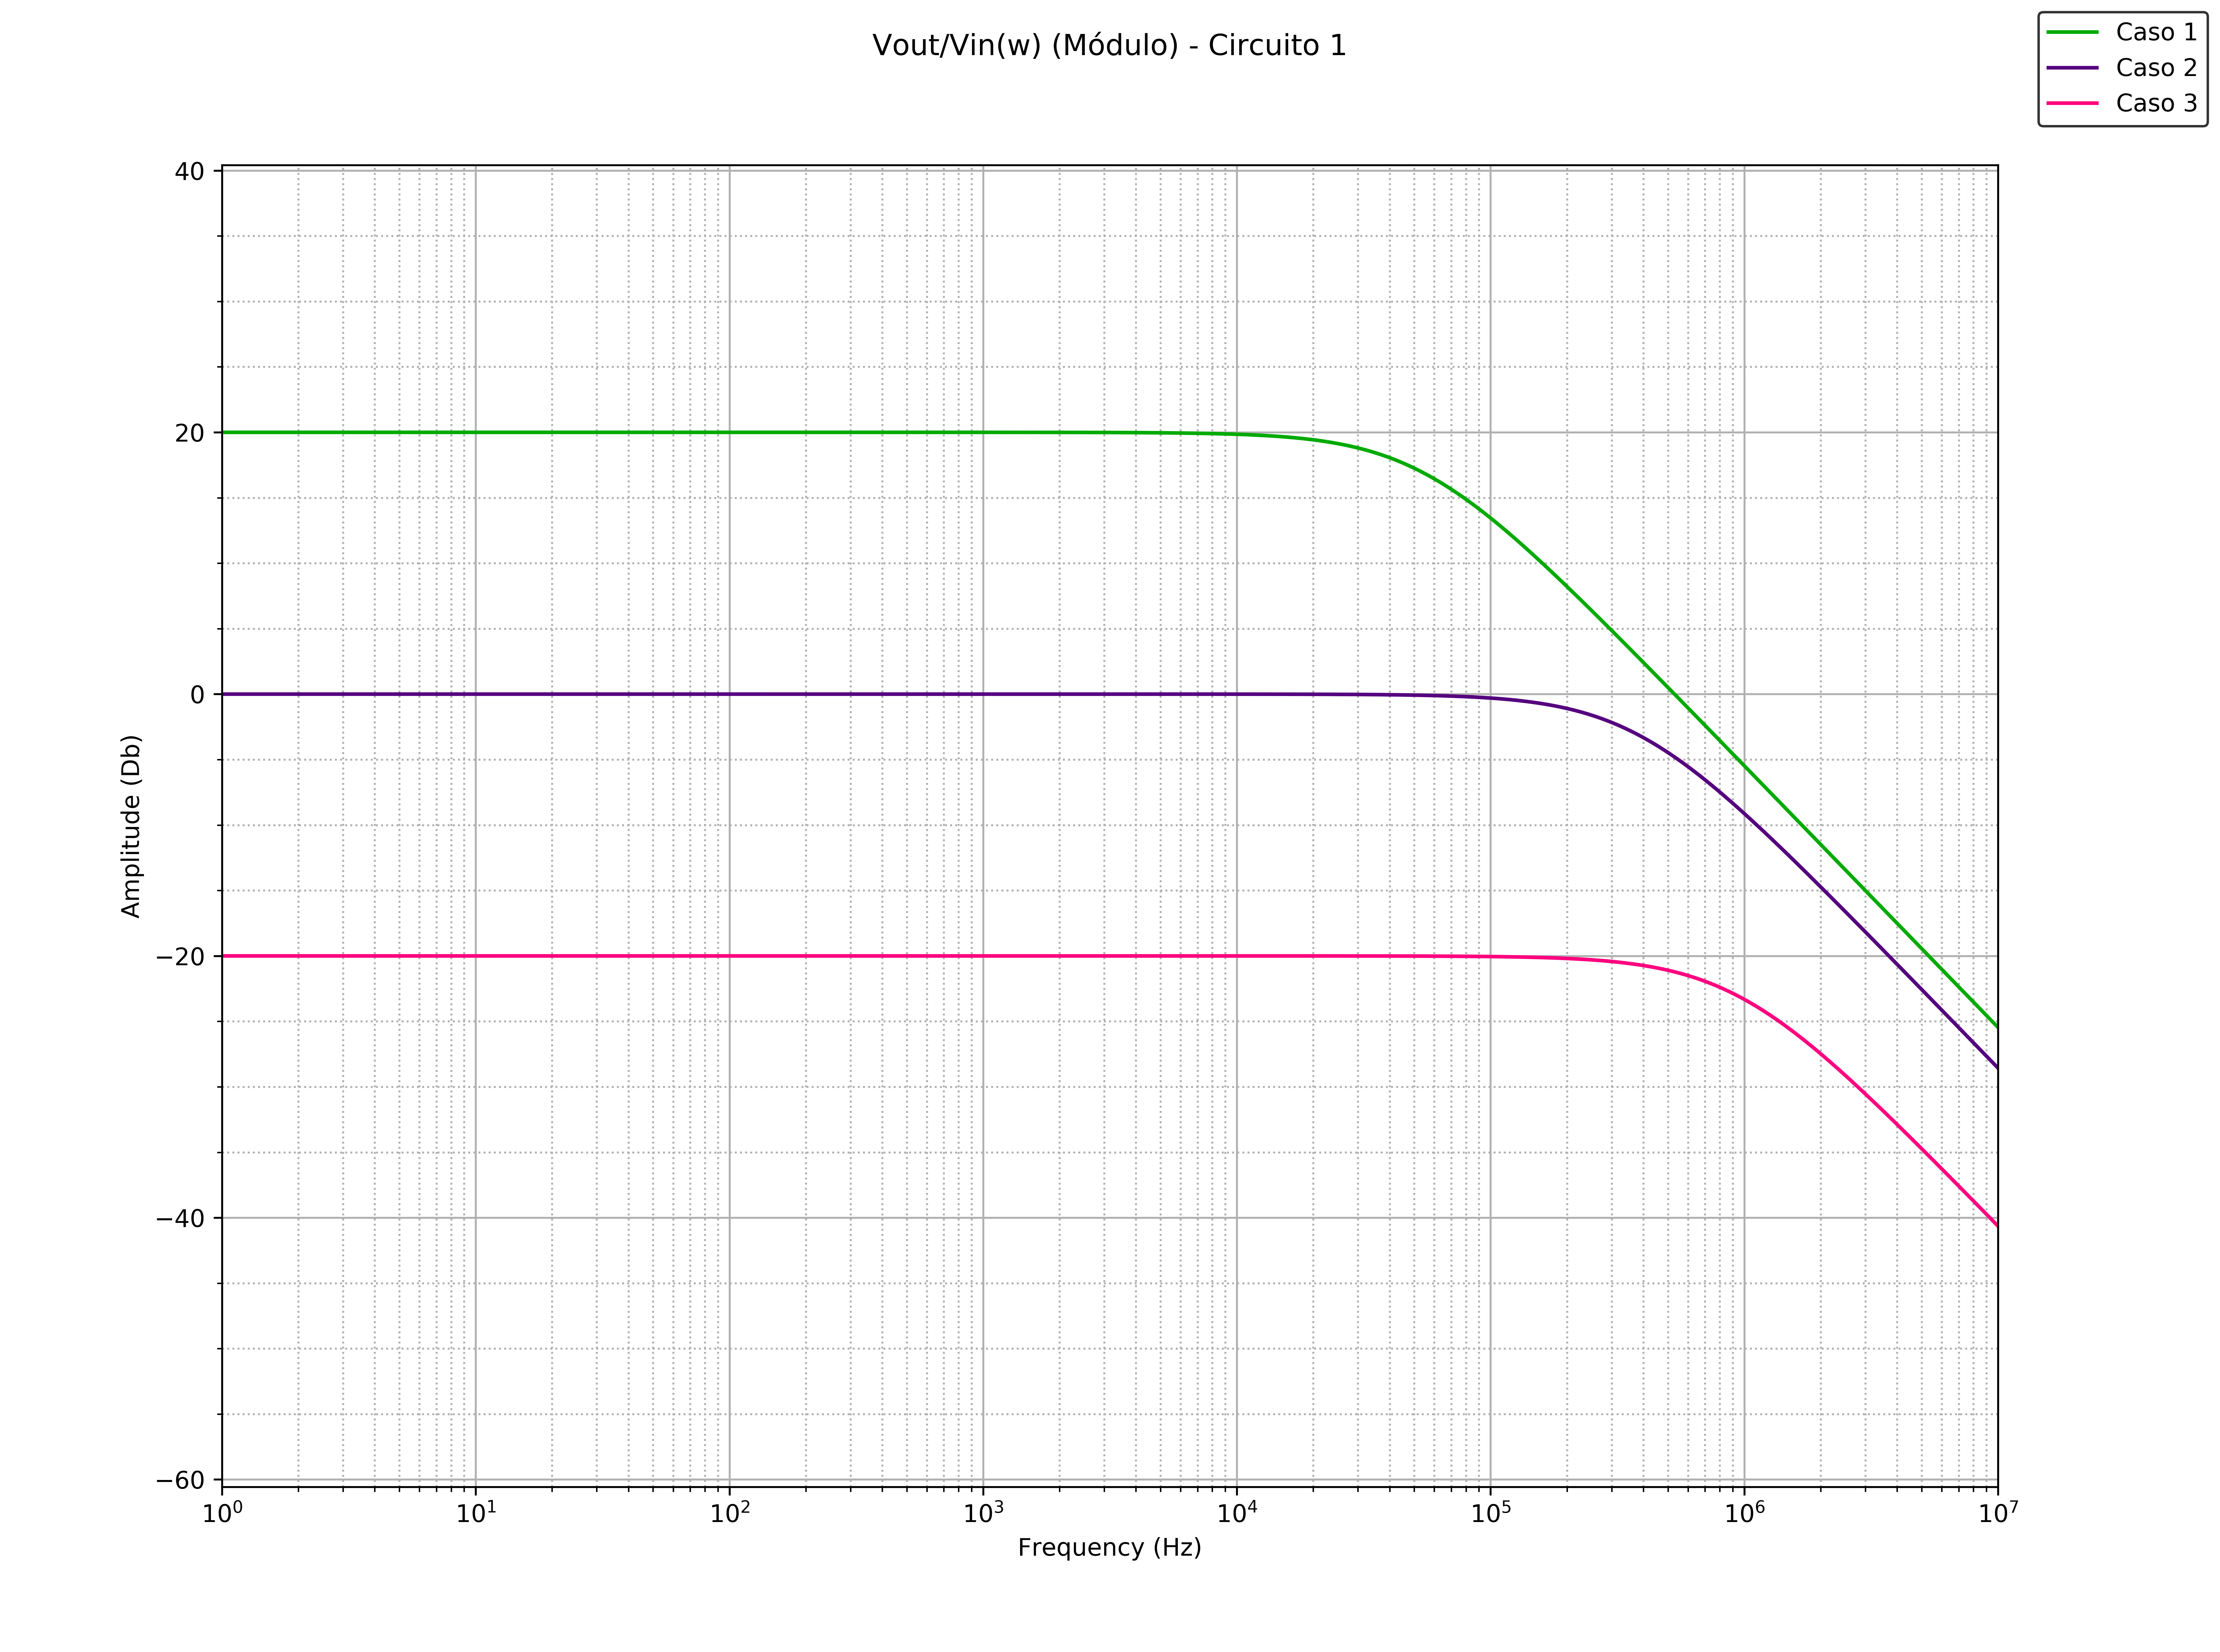
\includegraphics[scale=0.45]{../EJ1/00GRAFICOS/teoricos/circ1voviw.png}
	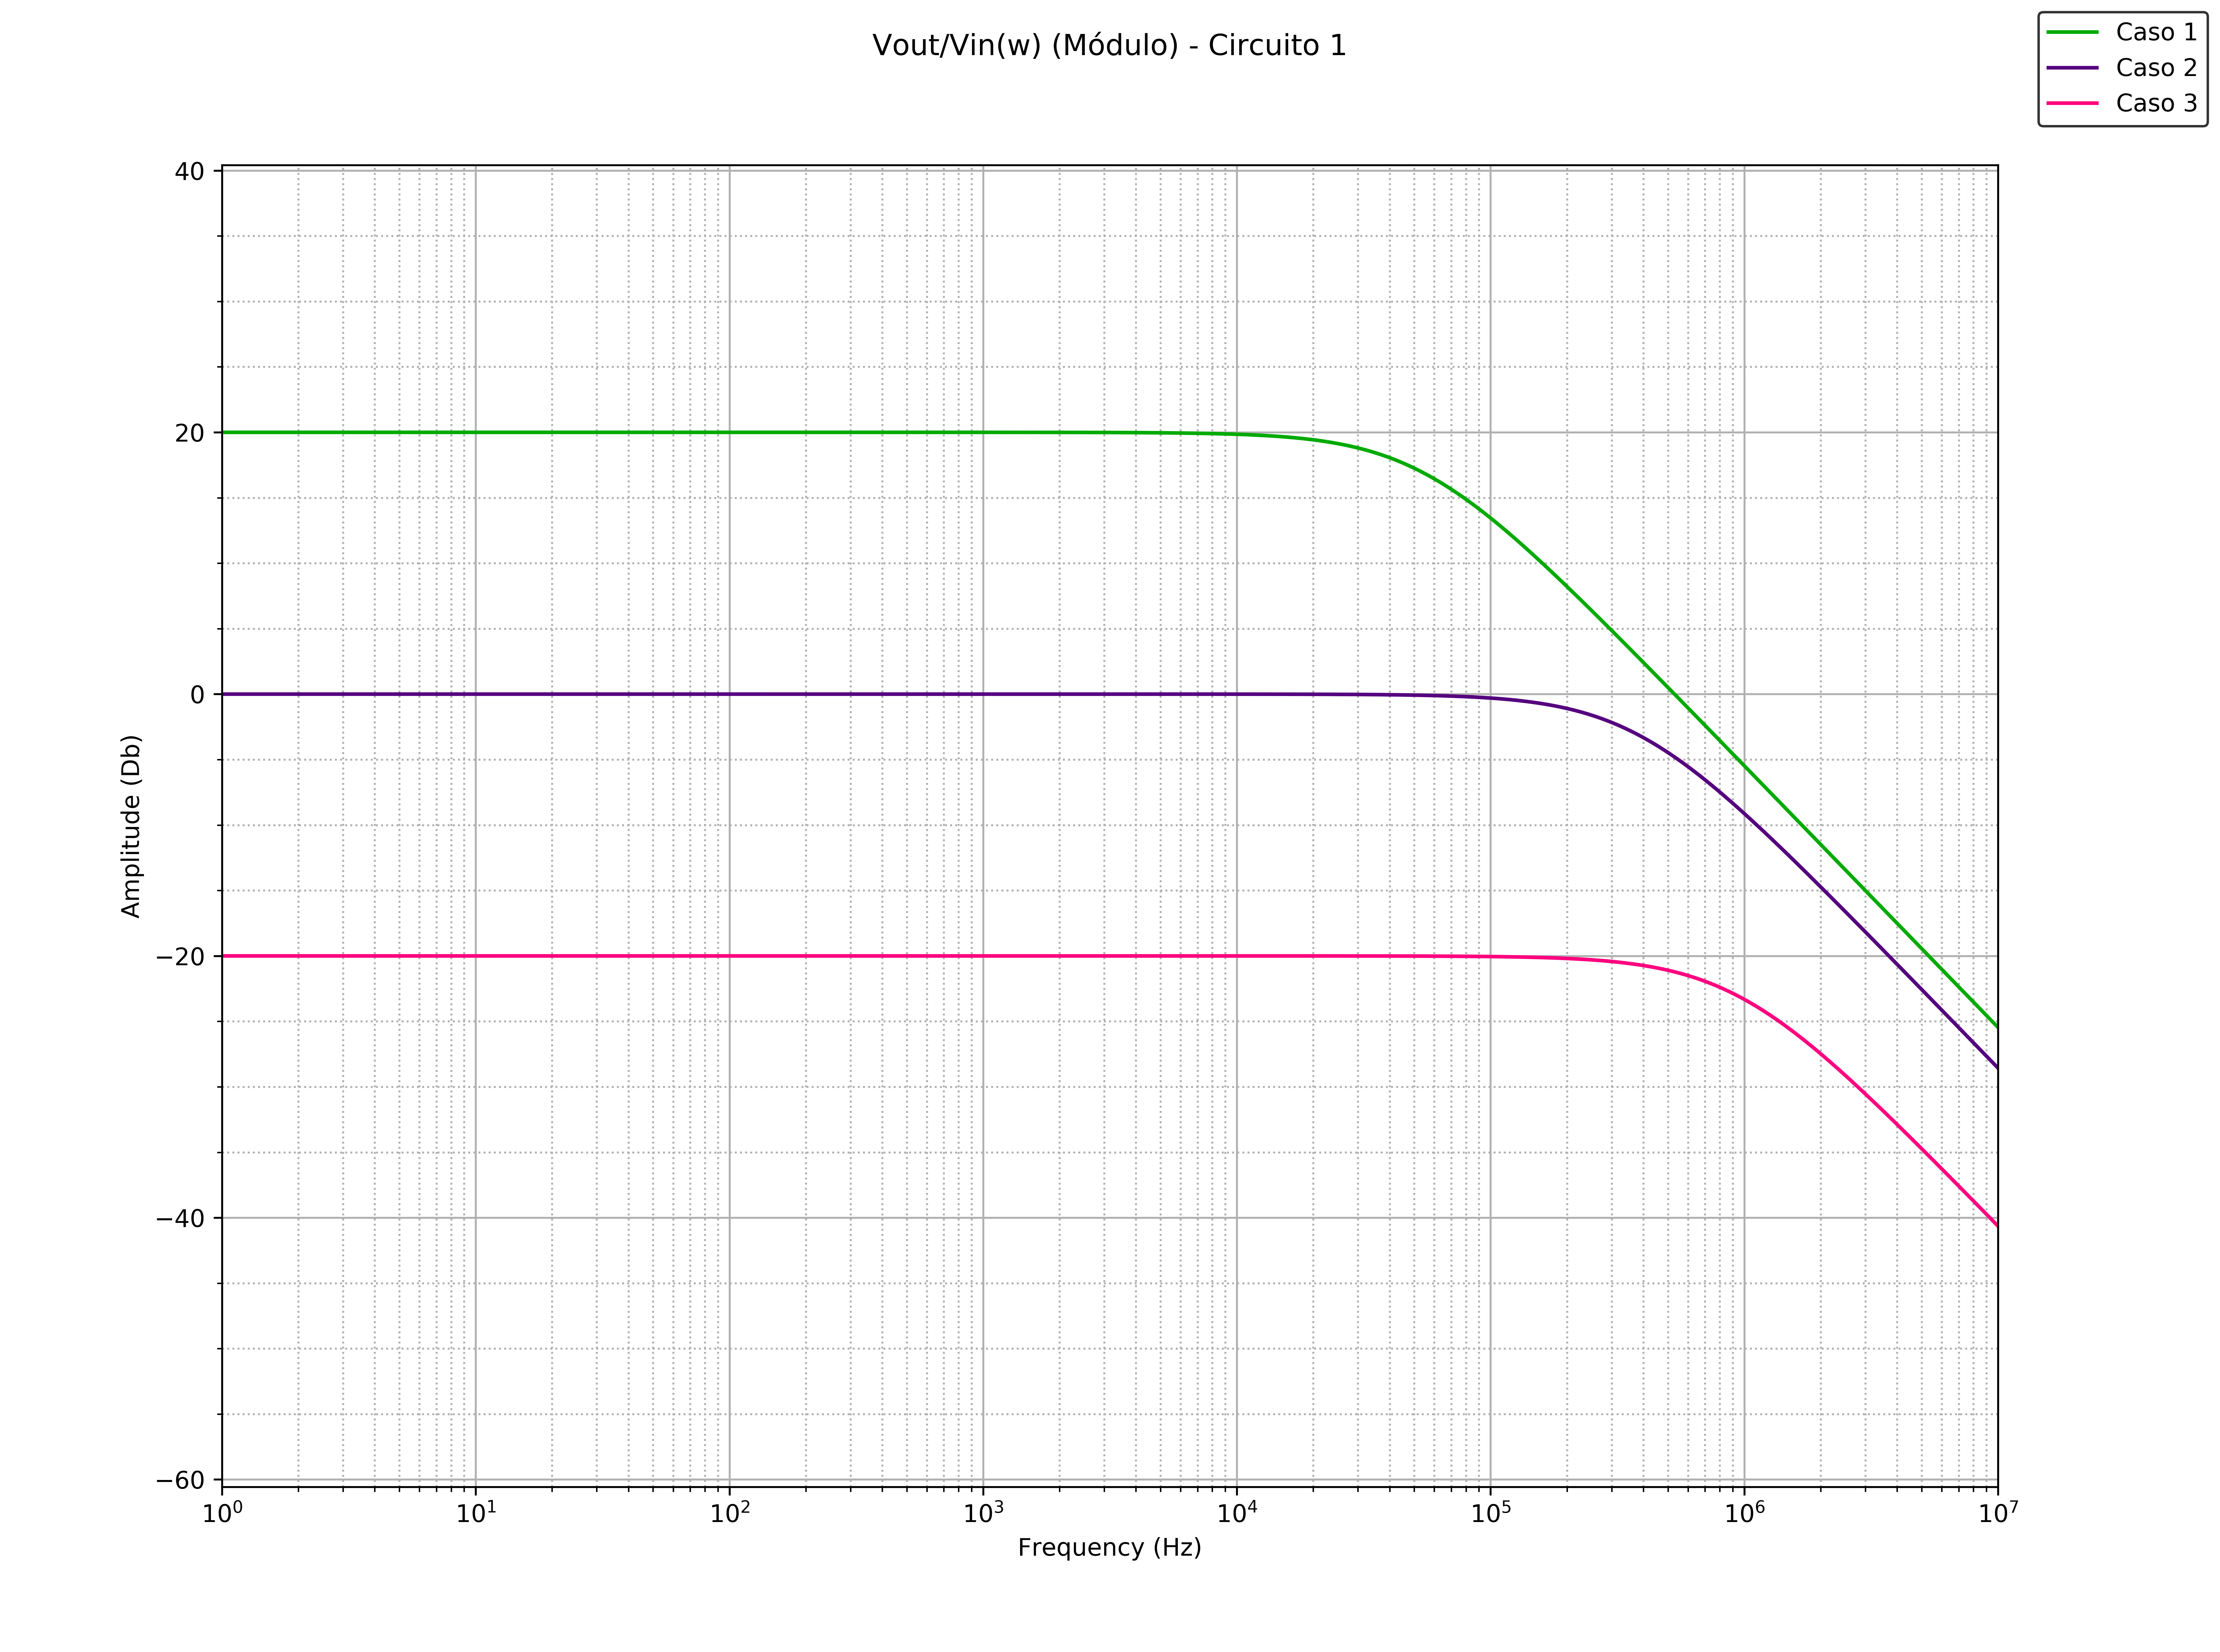
\includegraphics[width=10cm,height=10cm,keepaspectratio]{../EJ1/00GRAFICOS/teoricos/circ1voviw.png}
	\caption{Configuración inversora - Comparaci\'on te\'orica del m\'odulo de $V_{out}/V_{in}$ para los tres casos.}
	\label{c1voviTeoMod}
\end{figure}

\begin{figure}[H] %!ht
	\centering
	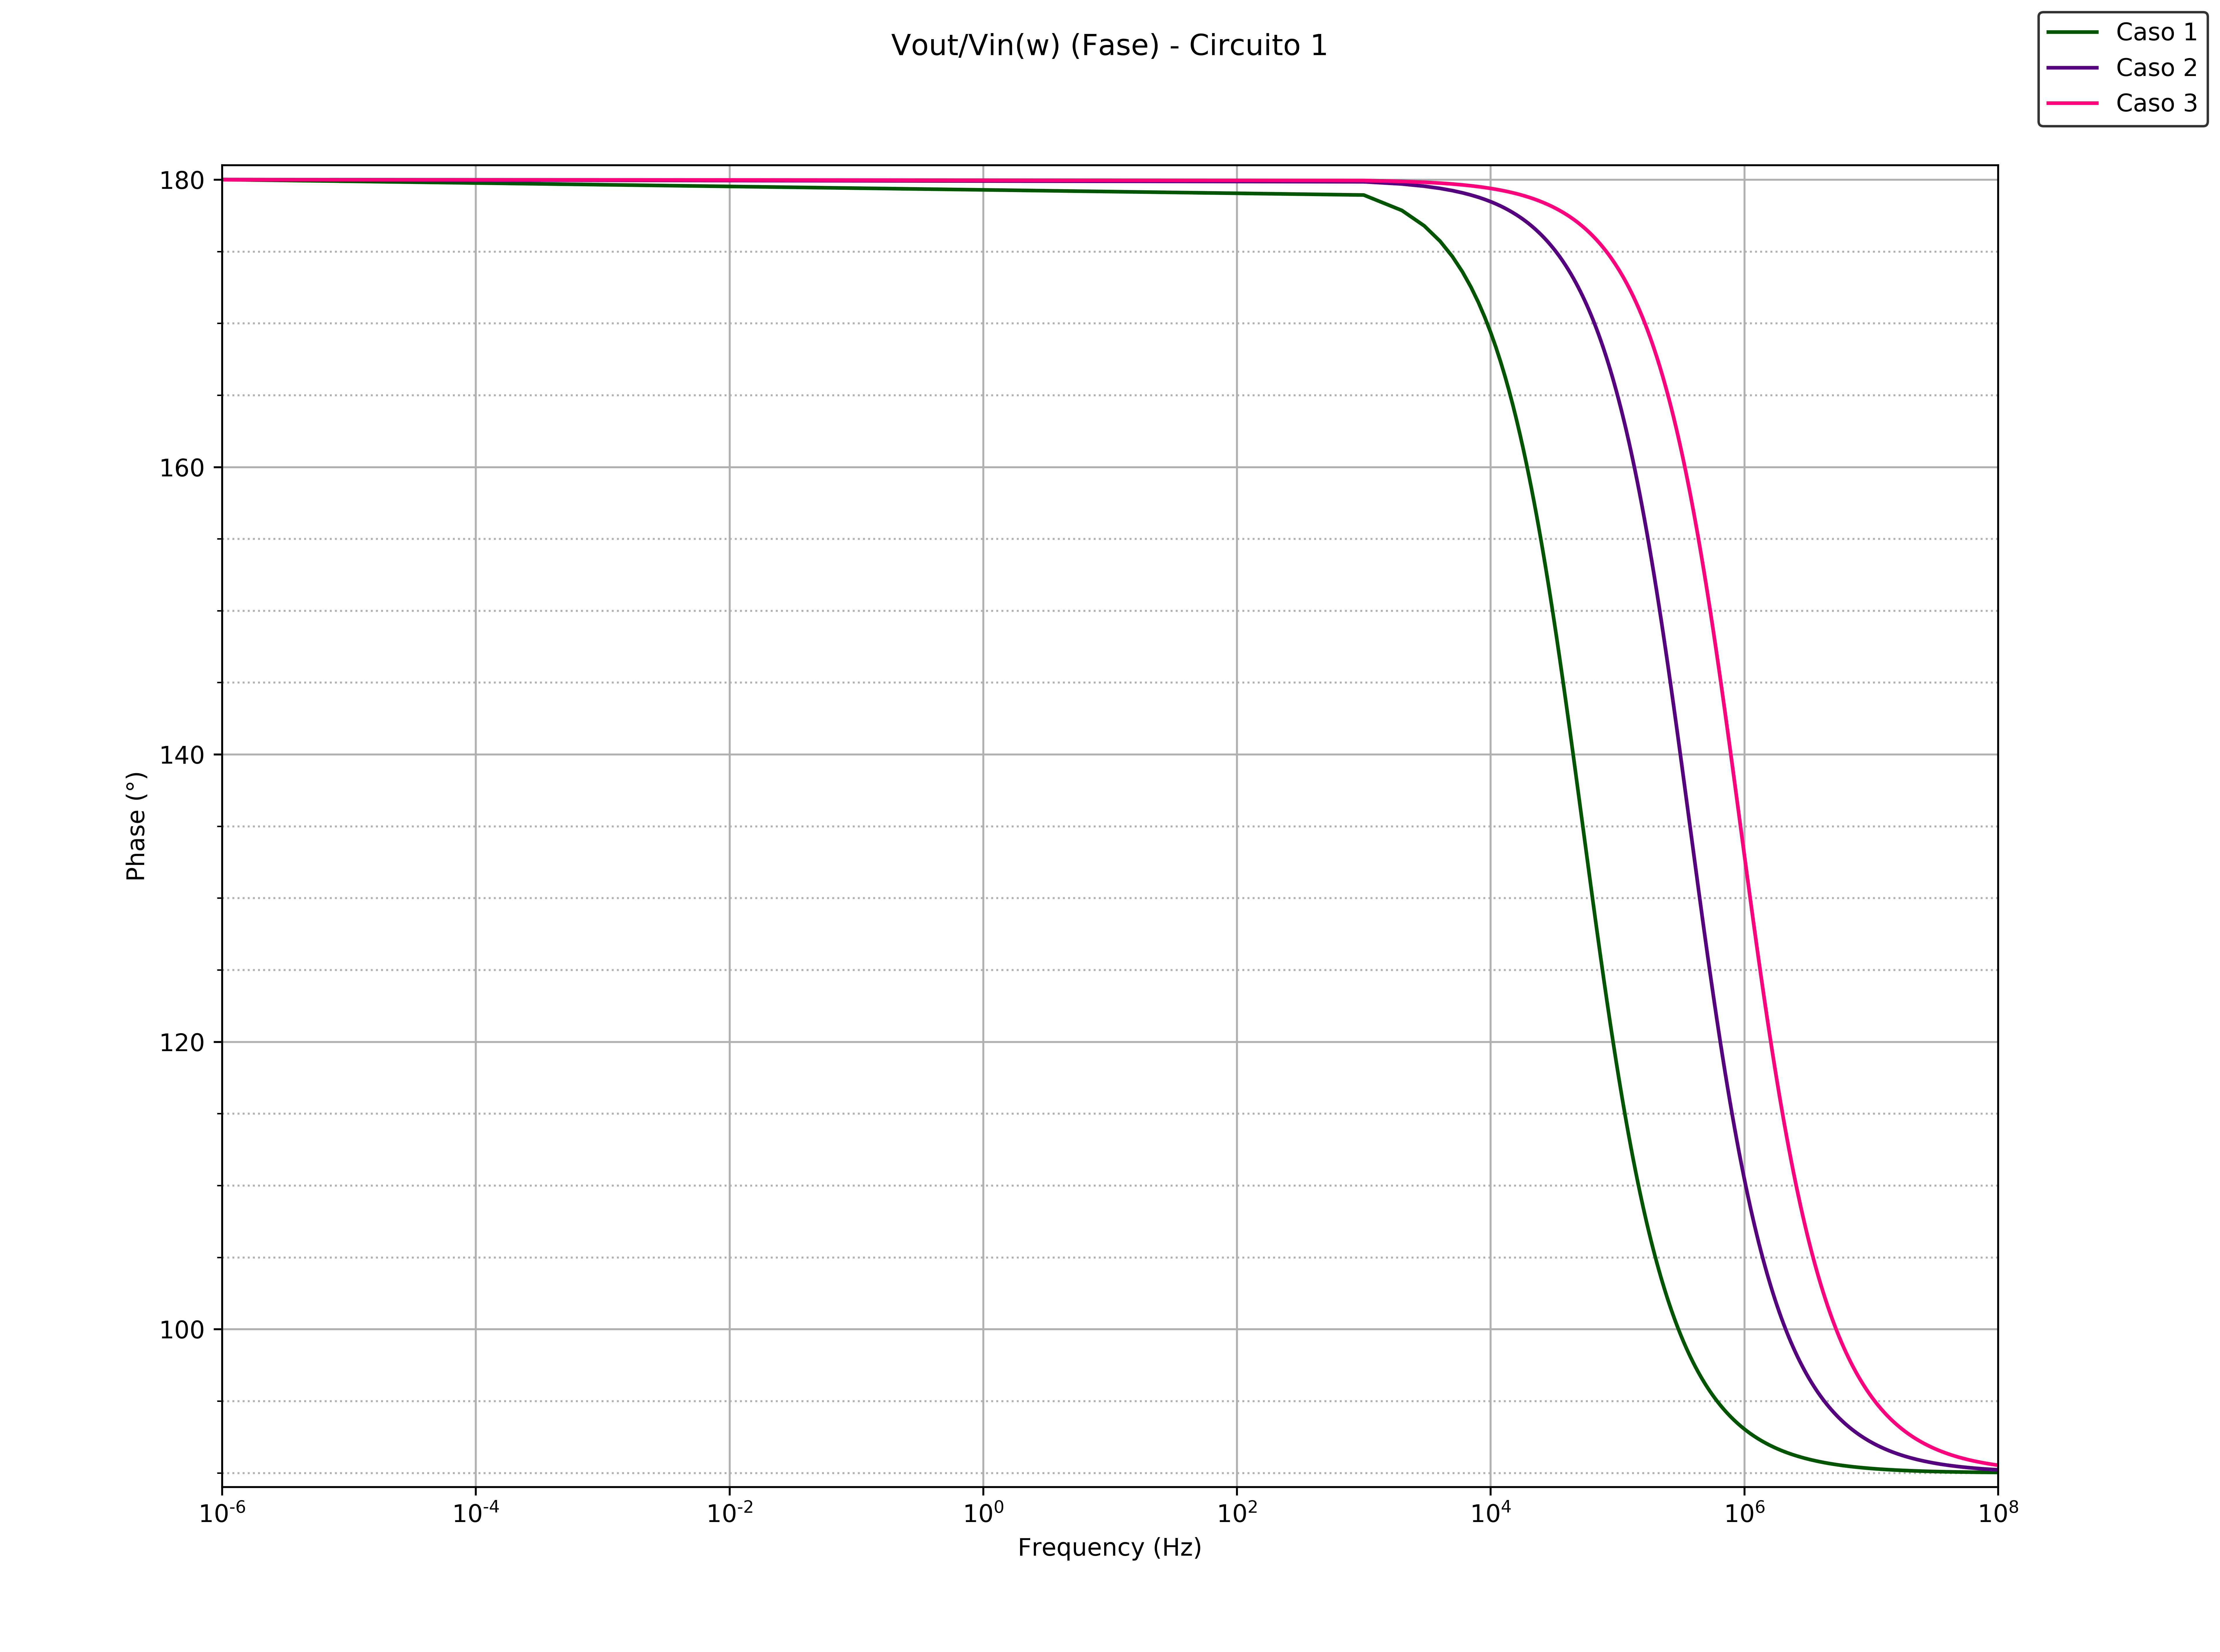
\includegraphics[width=10cm,height=10cm,keepaspectratio]{../EJ1/00GRAFICOS/teoricos/circ1vovifasew.png}
	\caption{Configuración inversora - Comparaci\'on te\'orica de la fase de $V_{out}/V_{in}$ para los tres casos.}
	\label{c1voviTeoPh}
\end{figure}

El gr\'afico \ref{c1voviTeoMod} permite ver una caracter\'istica importante que diferencia a los tres casos de resistencias para este circuito: la ganancia a bajas frecuencias. Las tres configuraciones corresponden a filtros pasabajos. Si bien aten\'uan a altas frecuencias, tienen comportamientos diferentes en las frecuencias bajas. Aqu\'el con resistencias para el caso 1 presenta una ganancia de 20dB, mientras que el del caso 3 aten\'ua 20 dB. El circuito del caso 2, por el contrario, no gana ni aten\'ua en frecuencias bajas.

%ANALIZAR AVOL FINITO . AVOL W ES LO QUE YA ESTA HECHO

\subsubsection*{Mediciones y resultados obtenidos} %%%%%%%

Se simul\'o y se midi\'o la ganancia para los tres casos del circuito \ref{c1} y a continuacio\'on se puede ver la diferencia entre sus resultados y los de las ecuaciones \ref{c1c1vovi}, \ref{c1c2vovi} y \ref{c1c3vovi}; correspondientes a la ganancia calculada de forma te\'orica y considerando al amplificador operacional como ideal.

\begin{figure}[H] %!ht
	\centering
	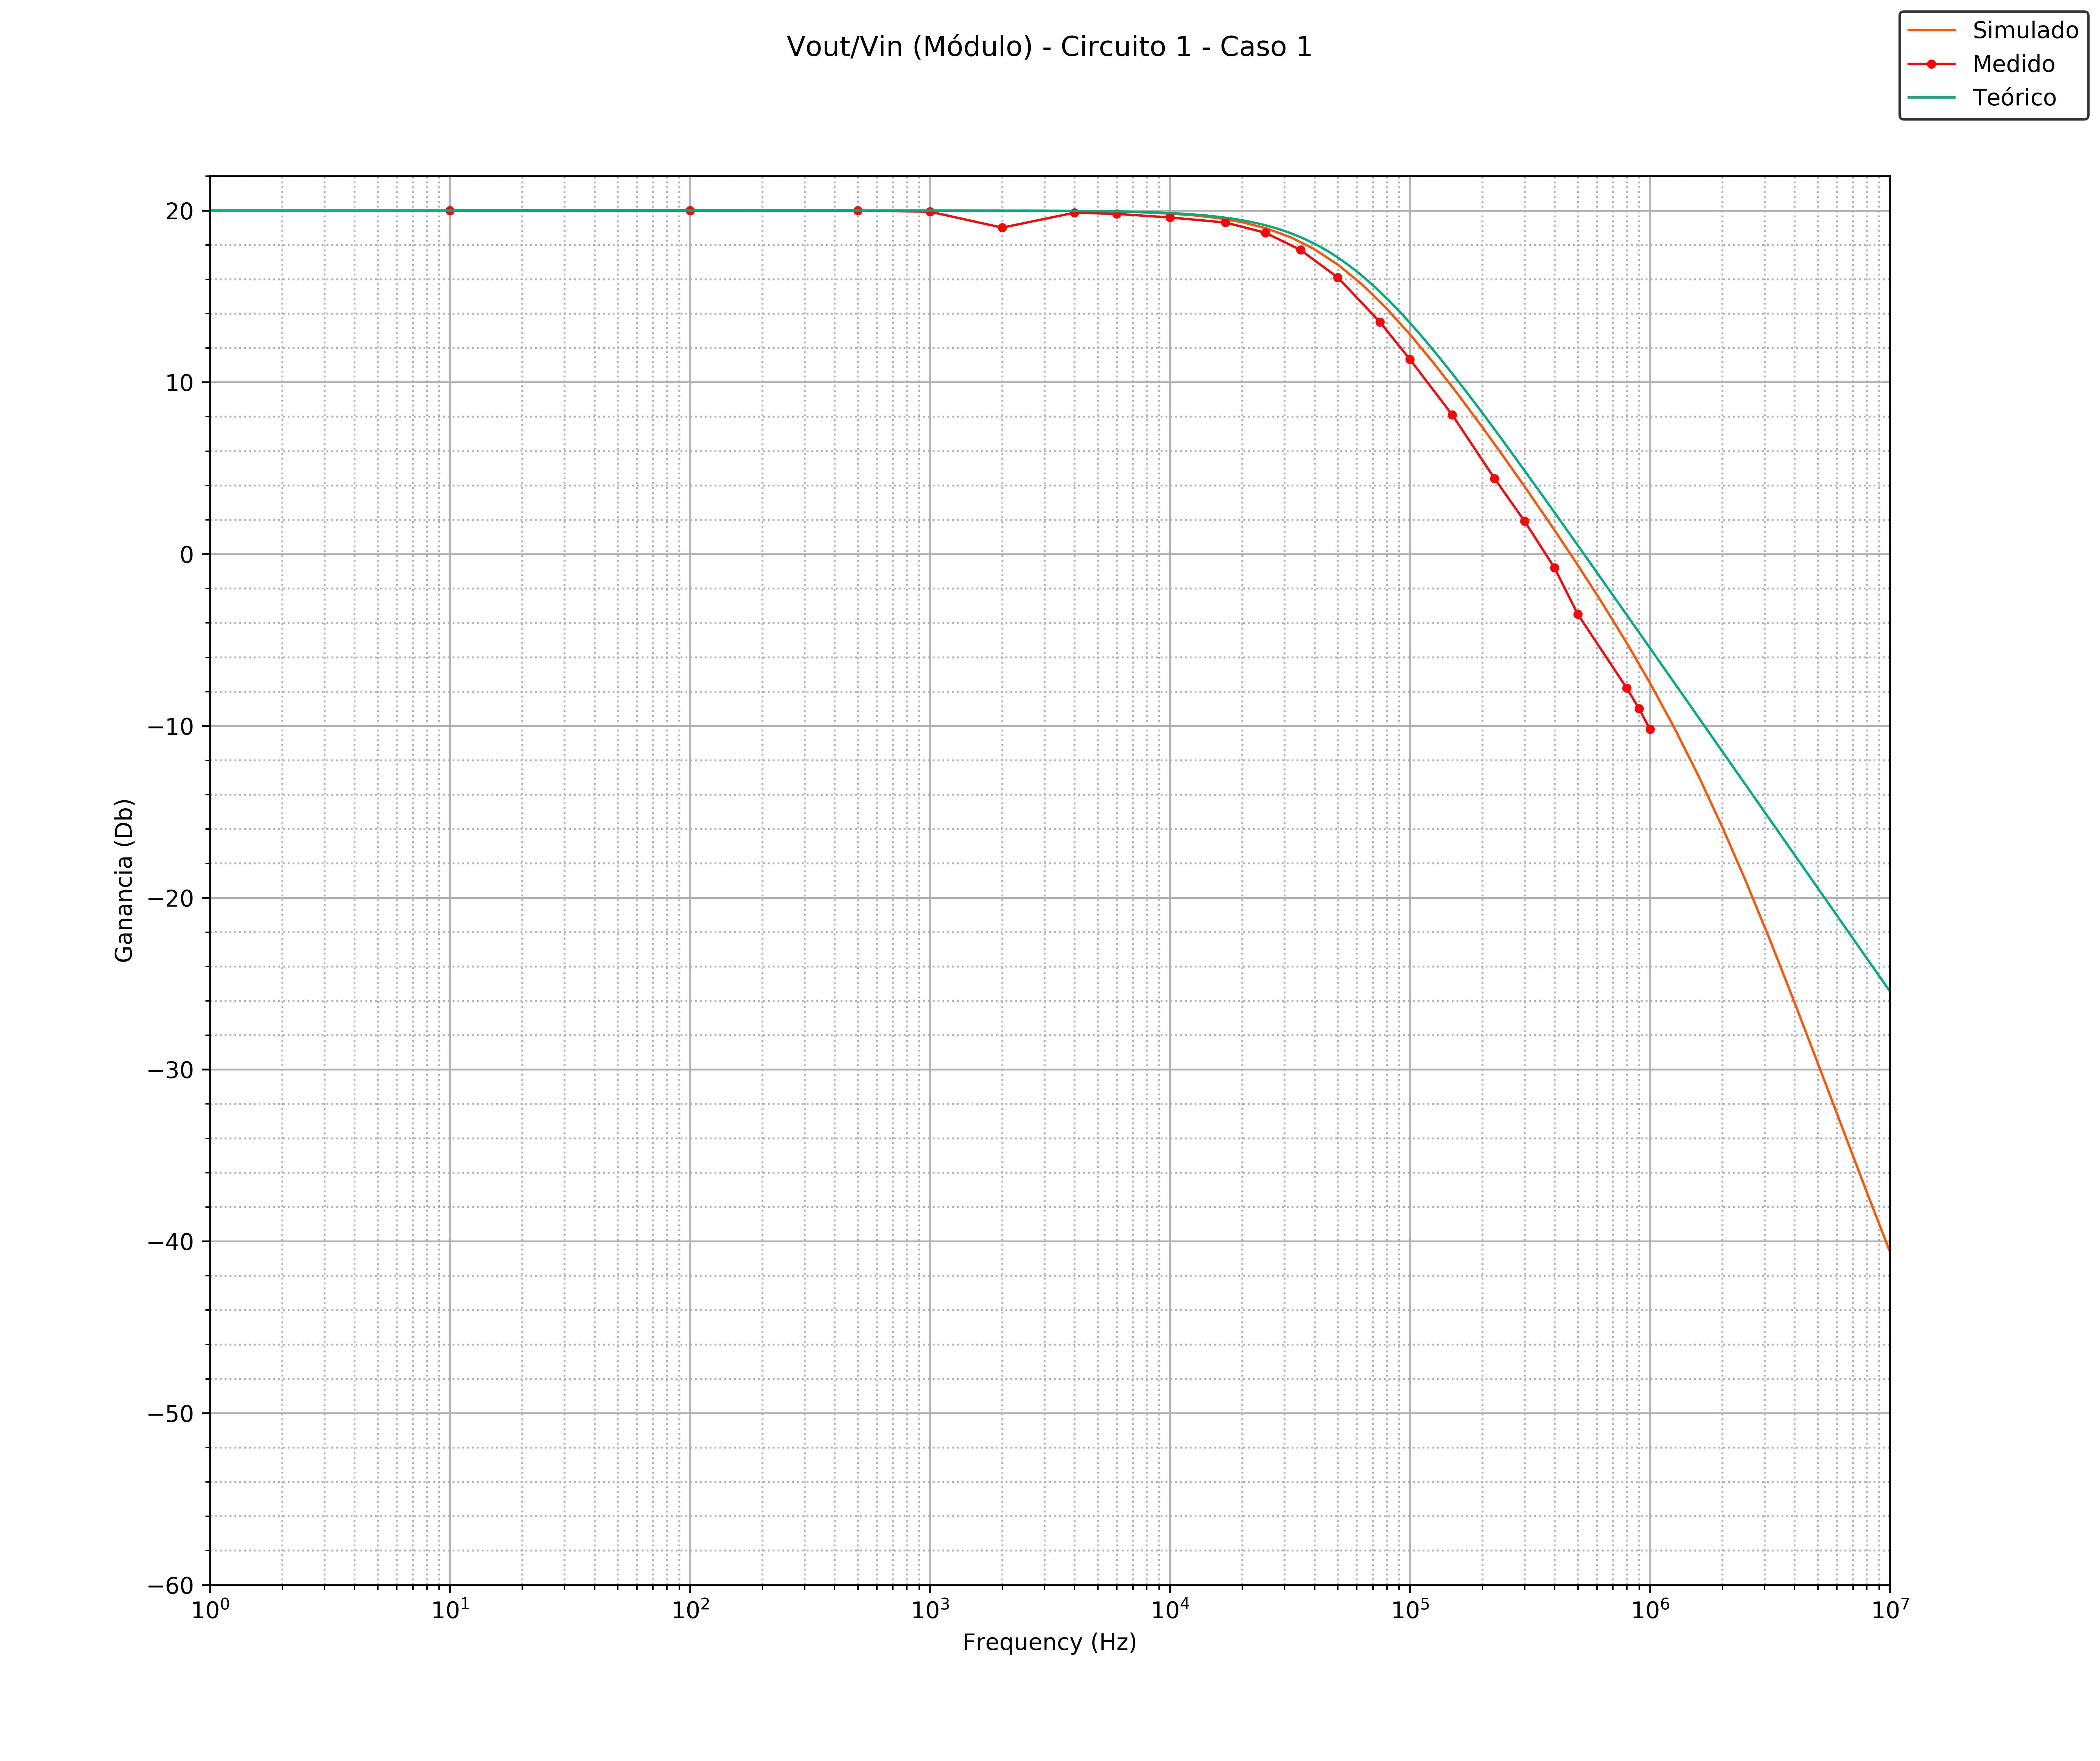
\includegraphics[width=10cm,height=10cm,keepaspectratio]{../EJ1/00GRAFICOS/c1c1/c1c1voviMod.png}
	\caption{Configuración inversora -  Caso 1 - Módulo de $V_{out}/V_{in}$}
	\label{c1c1voviM}
\end{figure}

\begin{figure}[H] %!ht
	\centering
	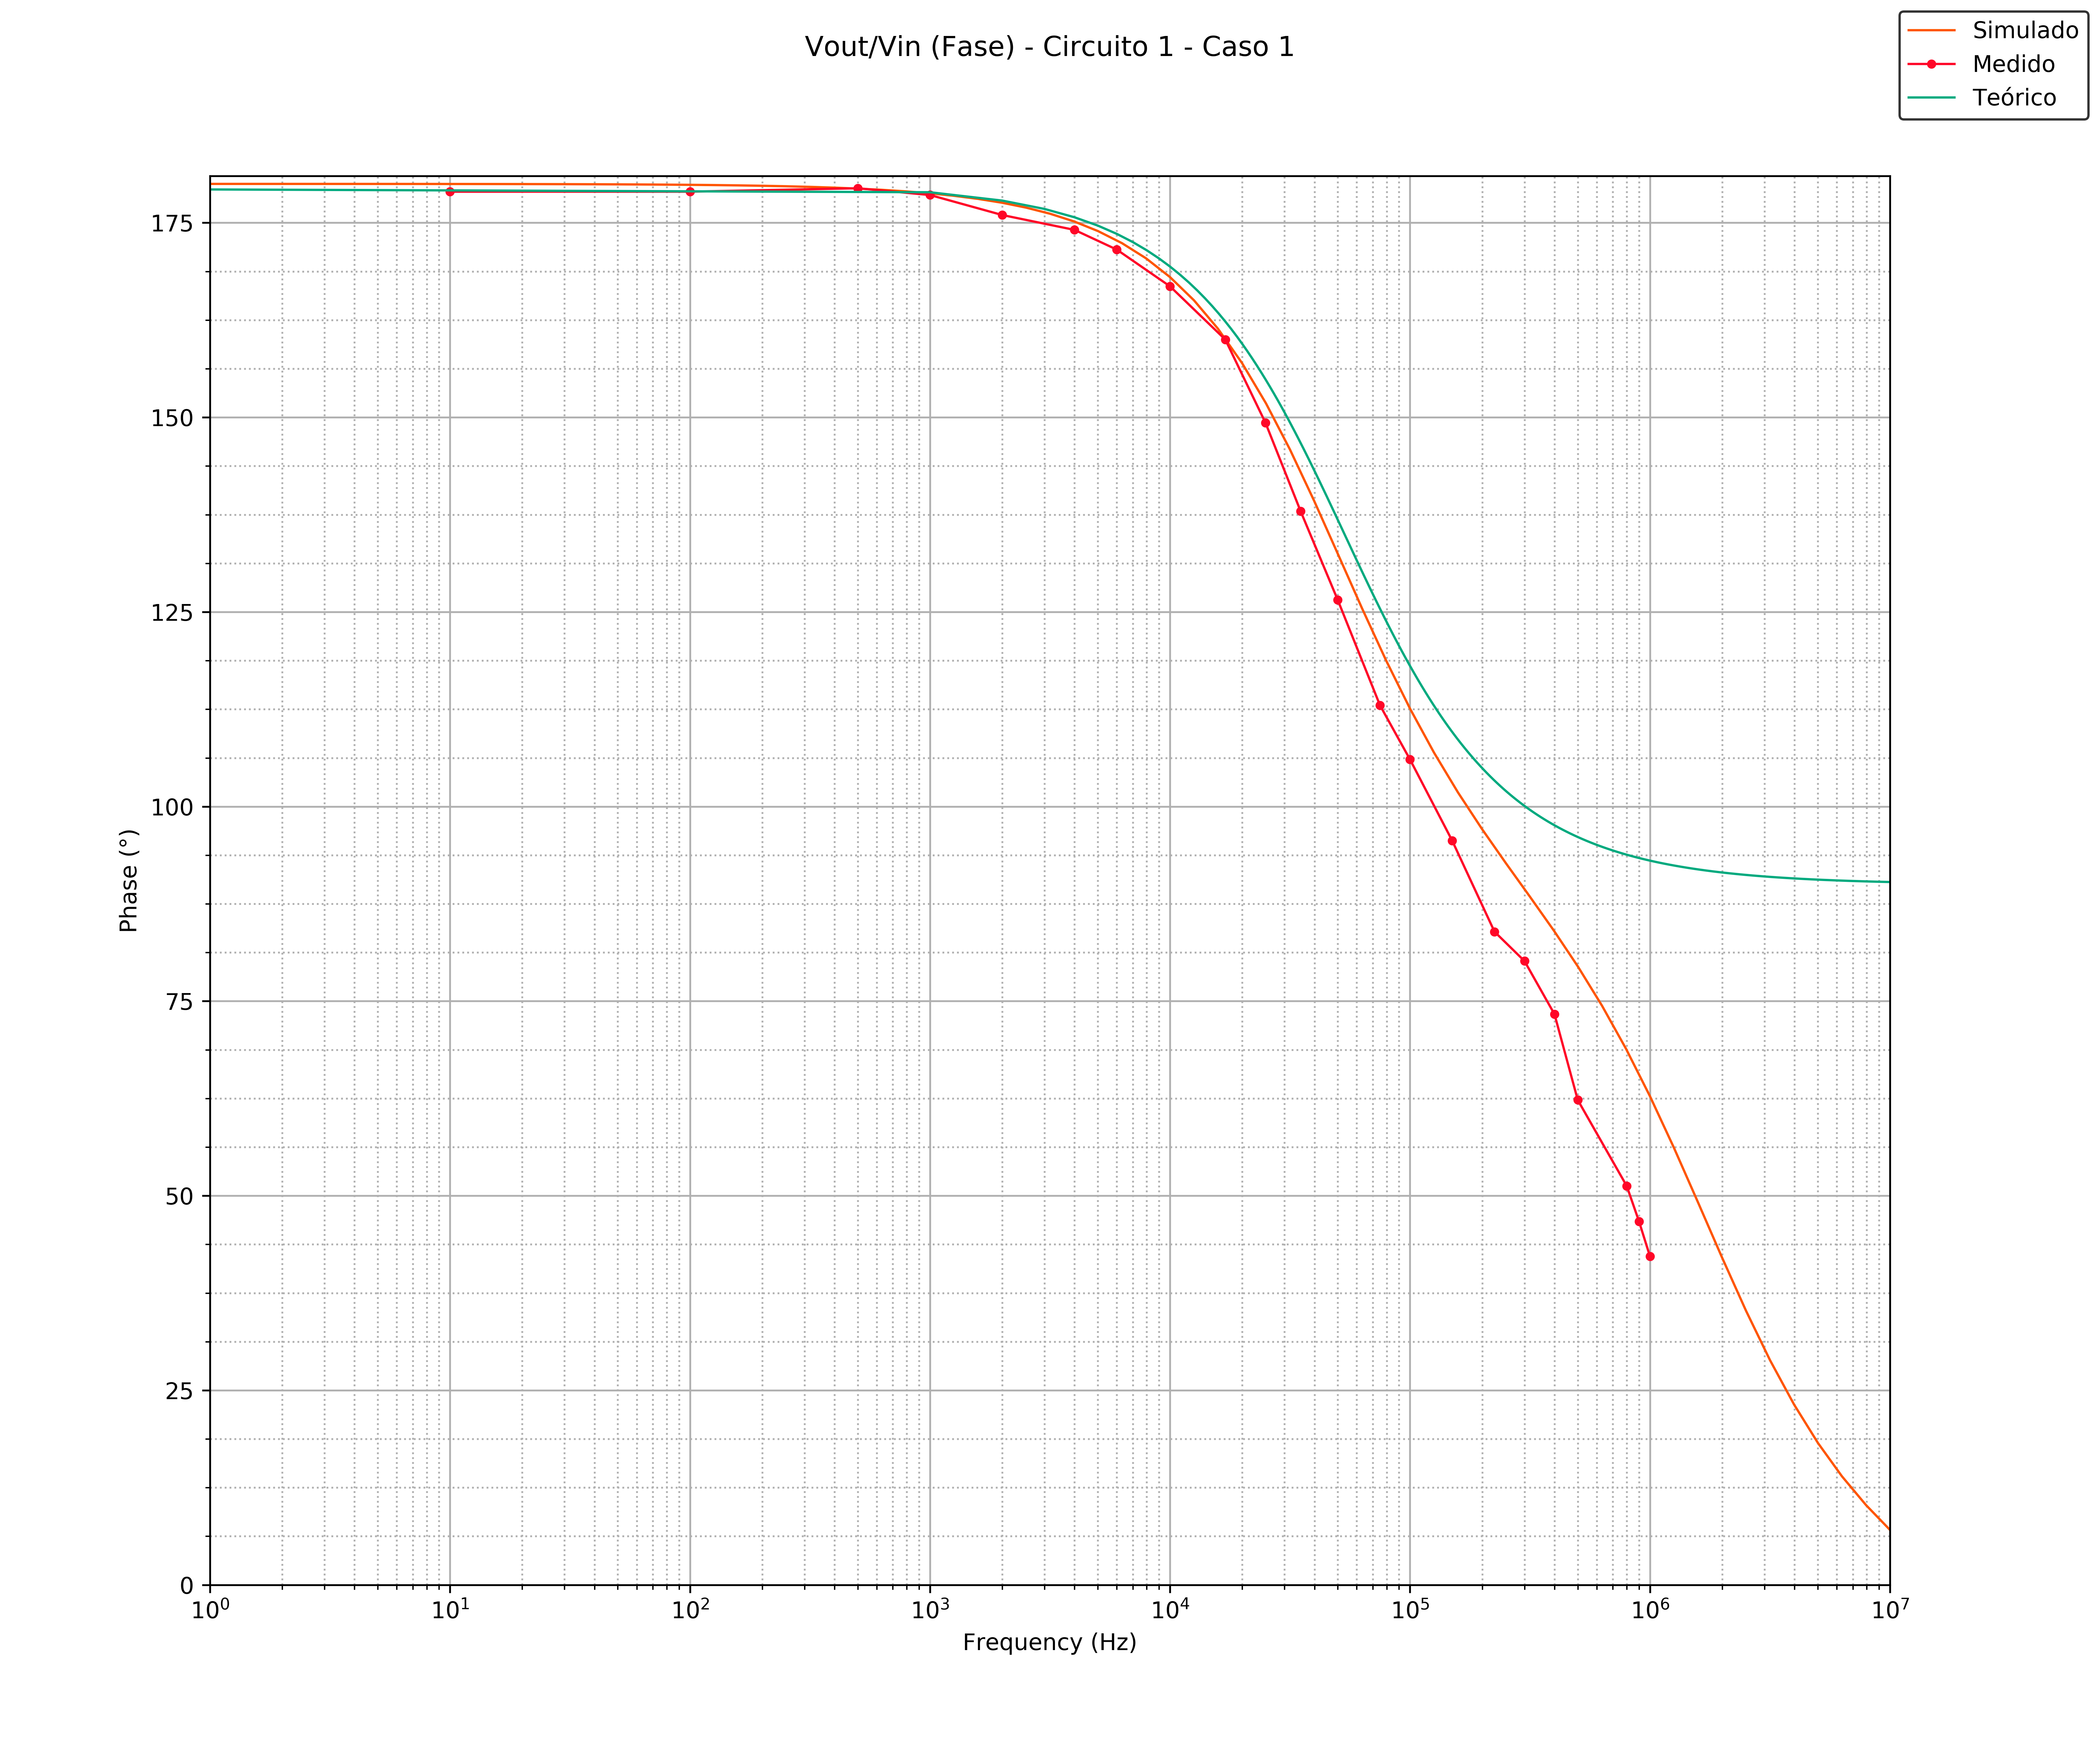
\includegraphics[width=10cm,height=10cm,keepaspectratio]{../EJ1/00GRAFICOS/c1c1/c1c1voviFASE.png}
	\caption{Configuración inversora - Caso 1 - Fase de $V_{out}/V_{in}$}
	\label{c1c1voviP}
\end{figure}

\begin{figure}[H] %!ht
	\centering
	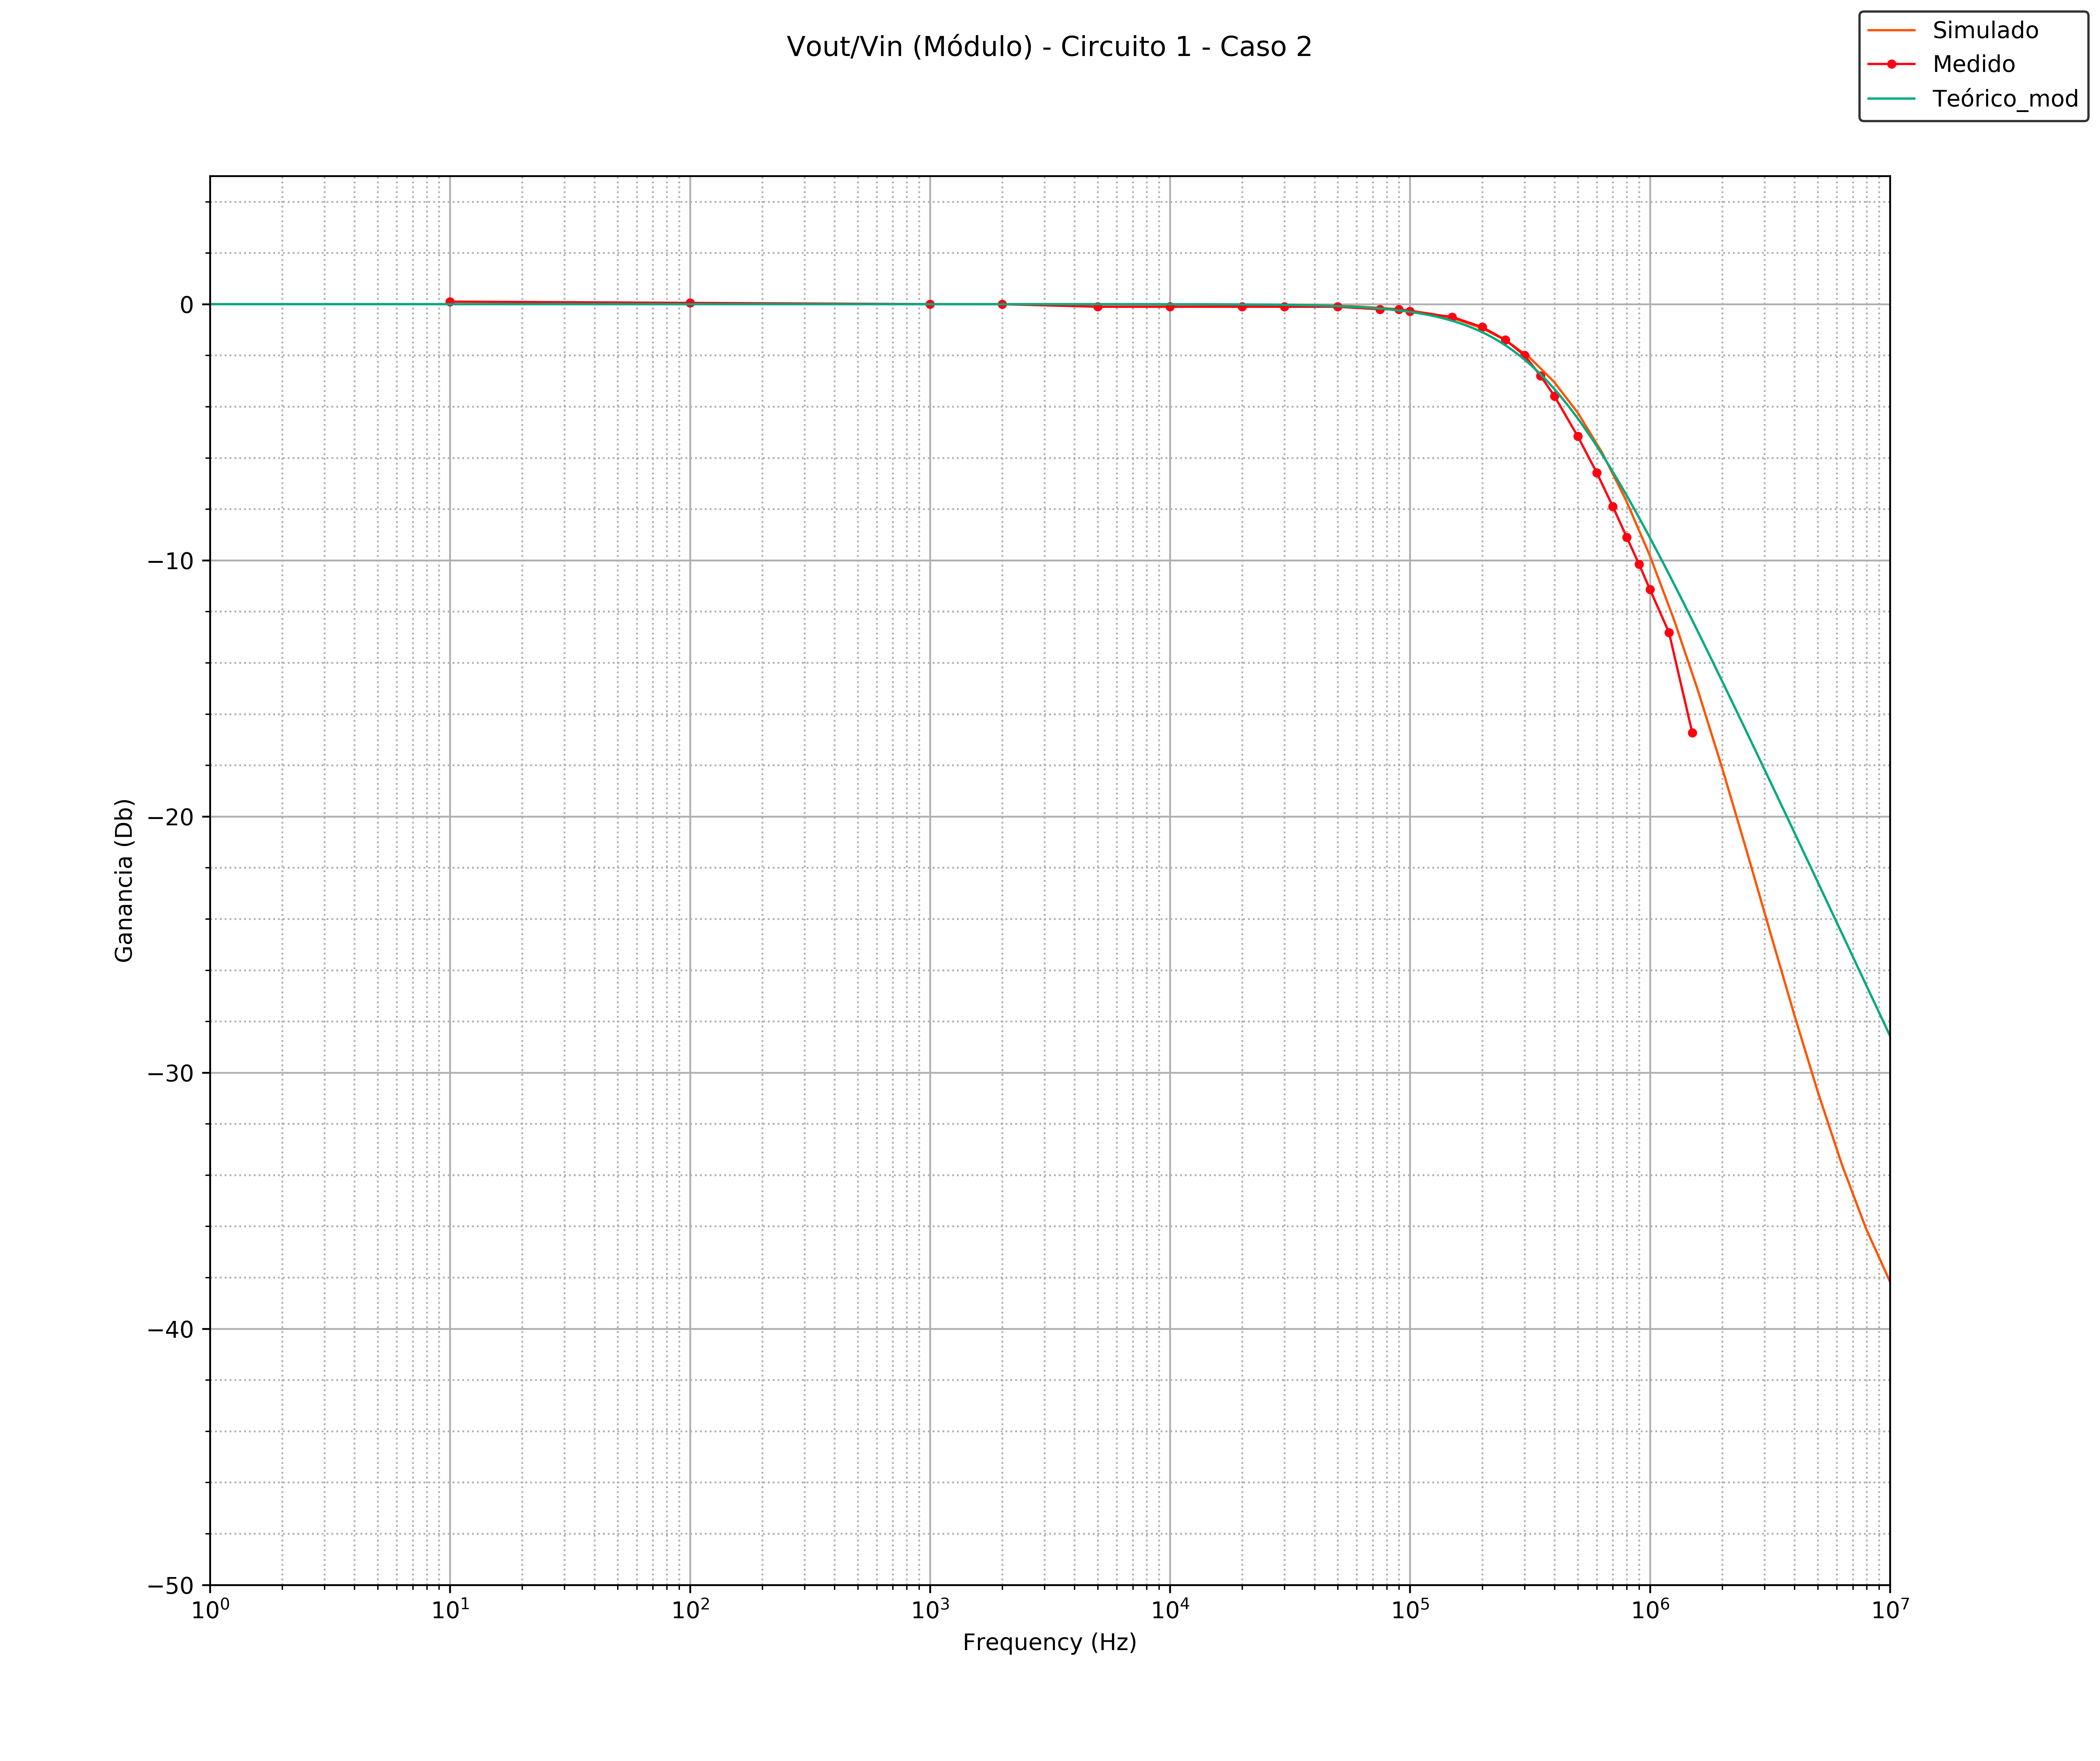
\includegraphics[width=10cm,height=10cm,keepaspectratio]{../EJ1/00GRAFICOS/c1c2/c1c2voviMod.png}
	\caption{Configuración inversora - Caso 2 - Módulo de $V_{out}/V_{in}$}
	\label{c1c2voviM}
\end{figure}

\begin{figure}[H] %!ht
	\centering
	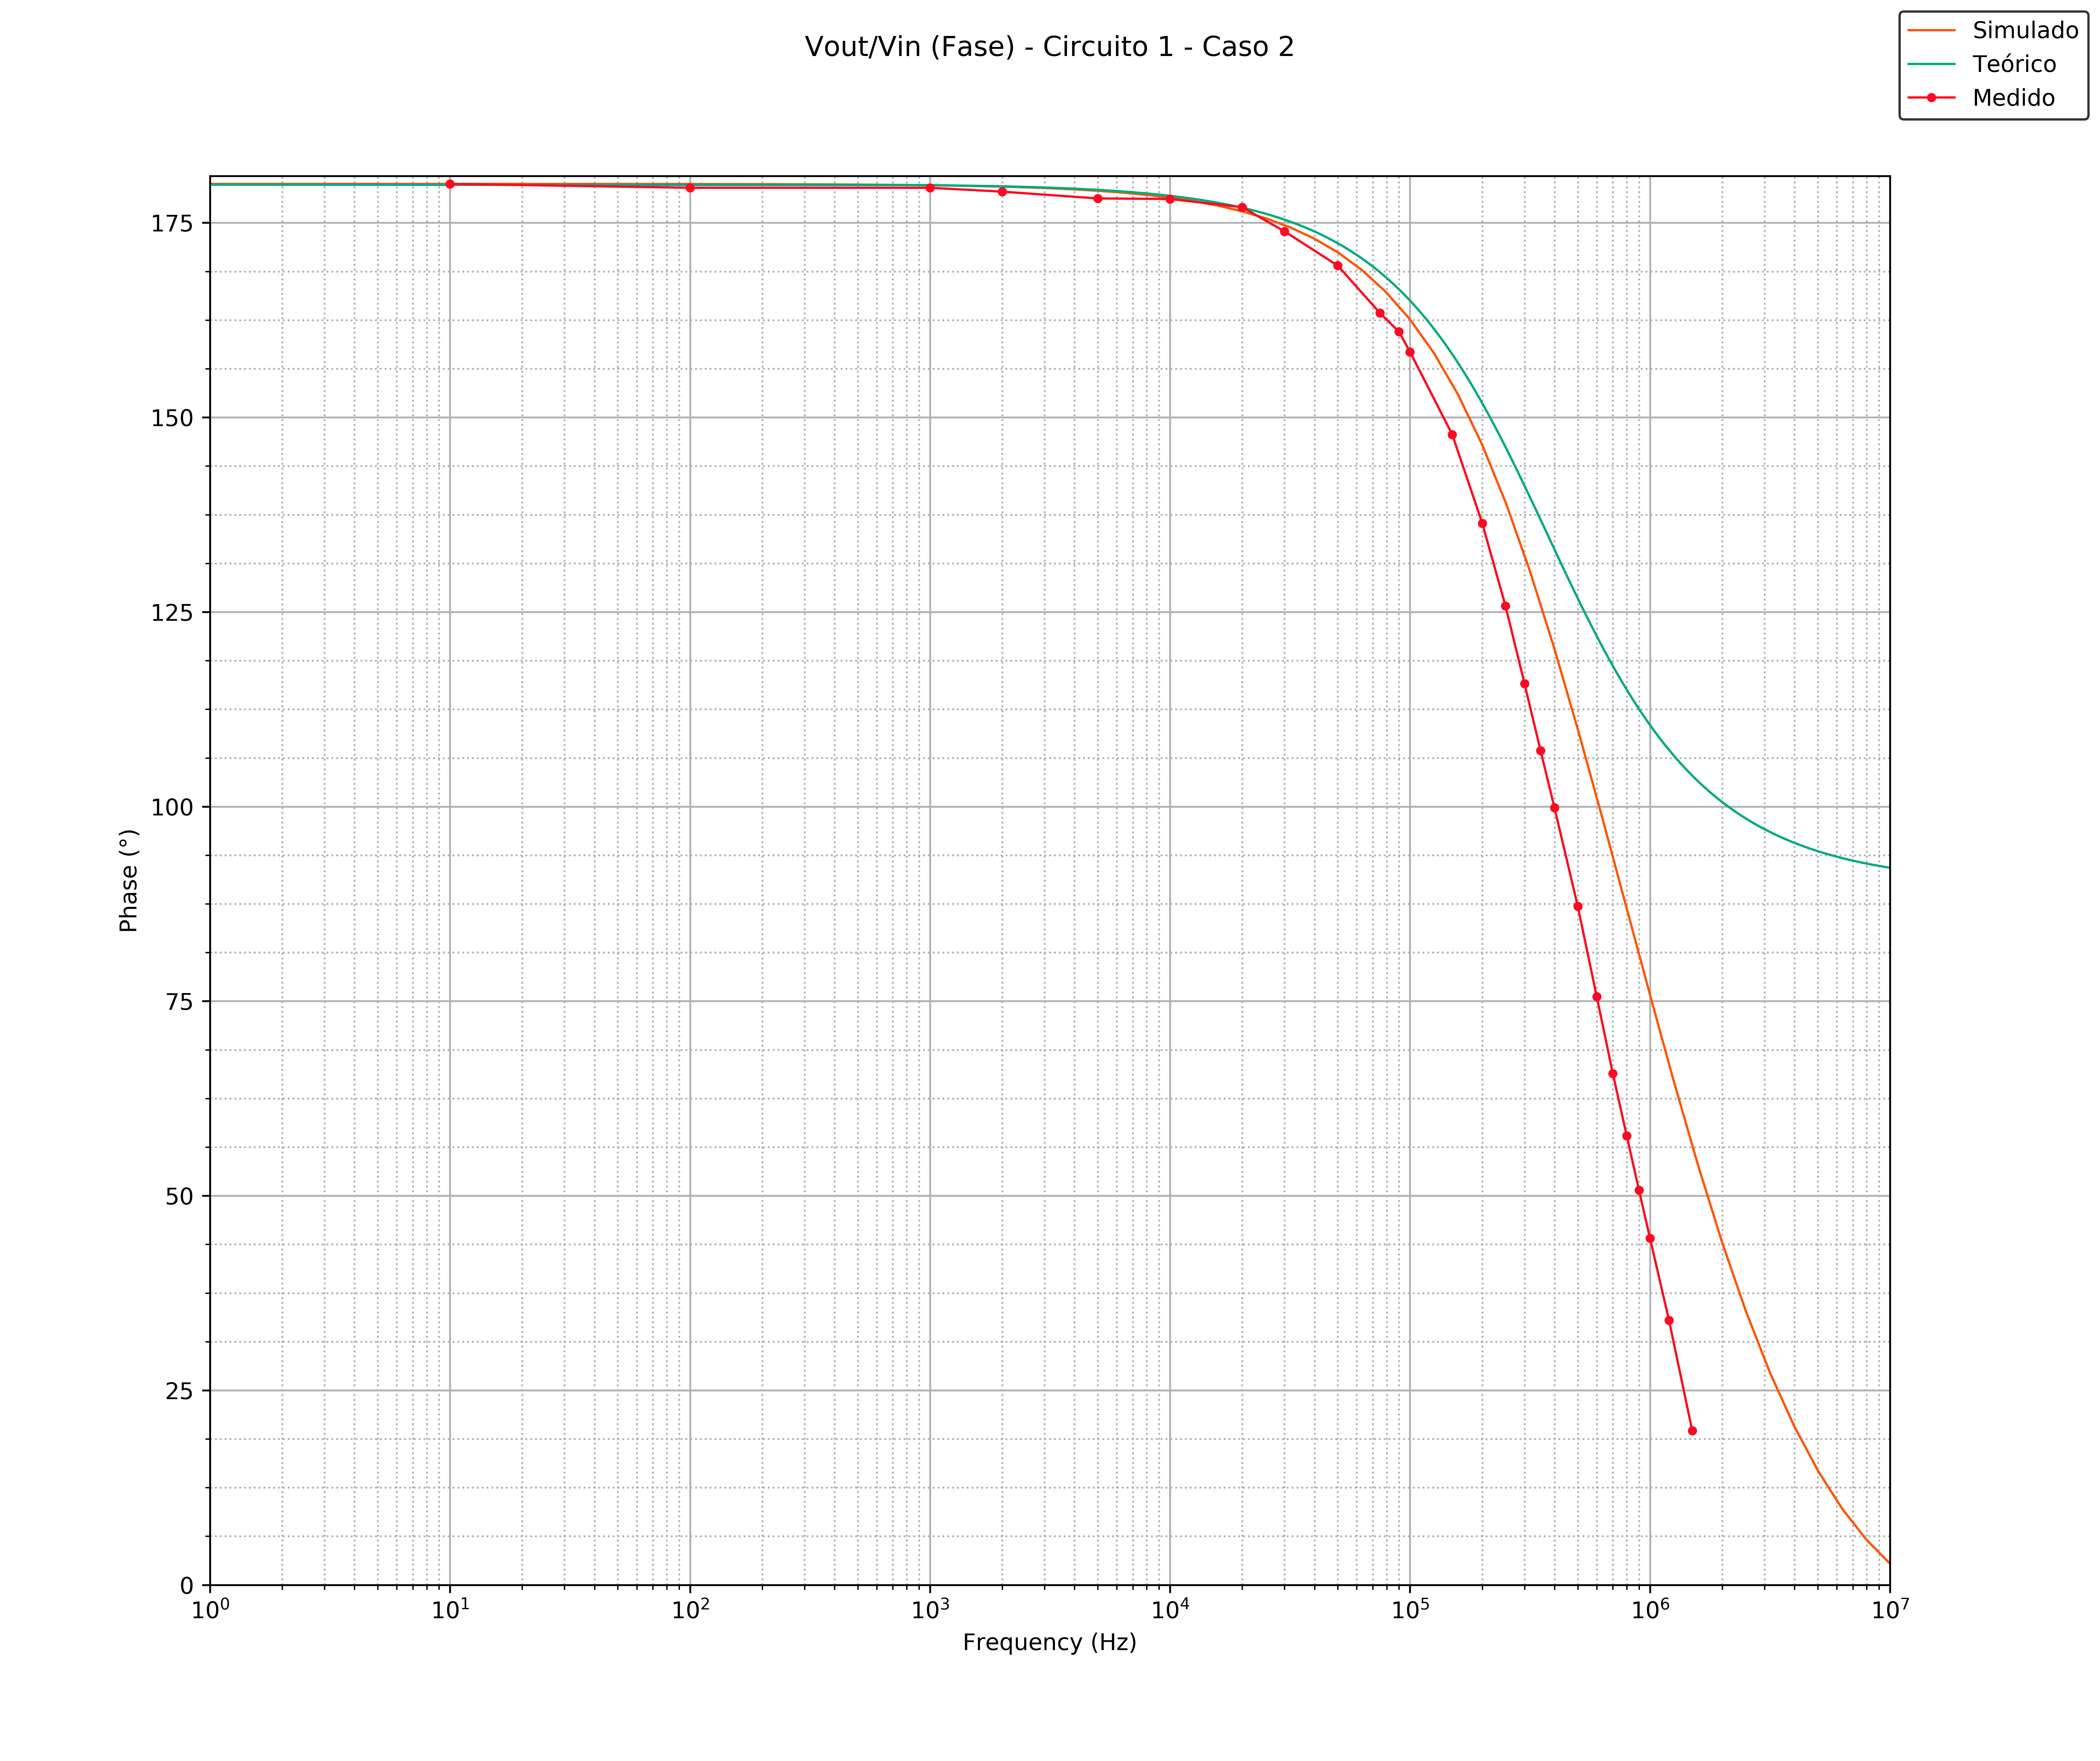
\includegraphics[width=10cm,height=10cm,keepaspectratio]{../EJ1/00GRAFICOS/c1c2/c1c2voviFASE.png}
	\caption{Configuración inversora - Caso 2 - Fase de $V_{out}/V_{in}$ }
	\label{c1c2voviP}
\end{figure}

\begin{figure}[H] %!ht
	\centering
	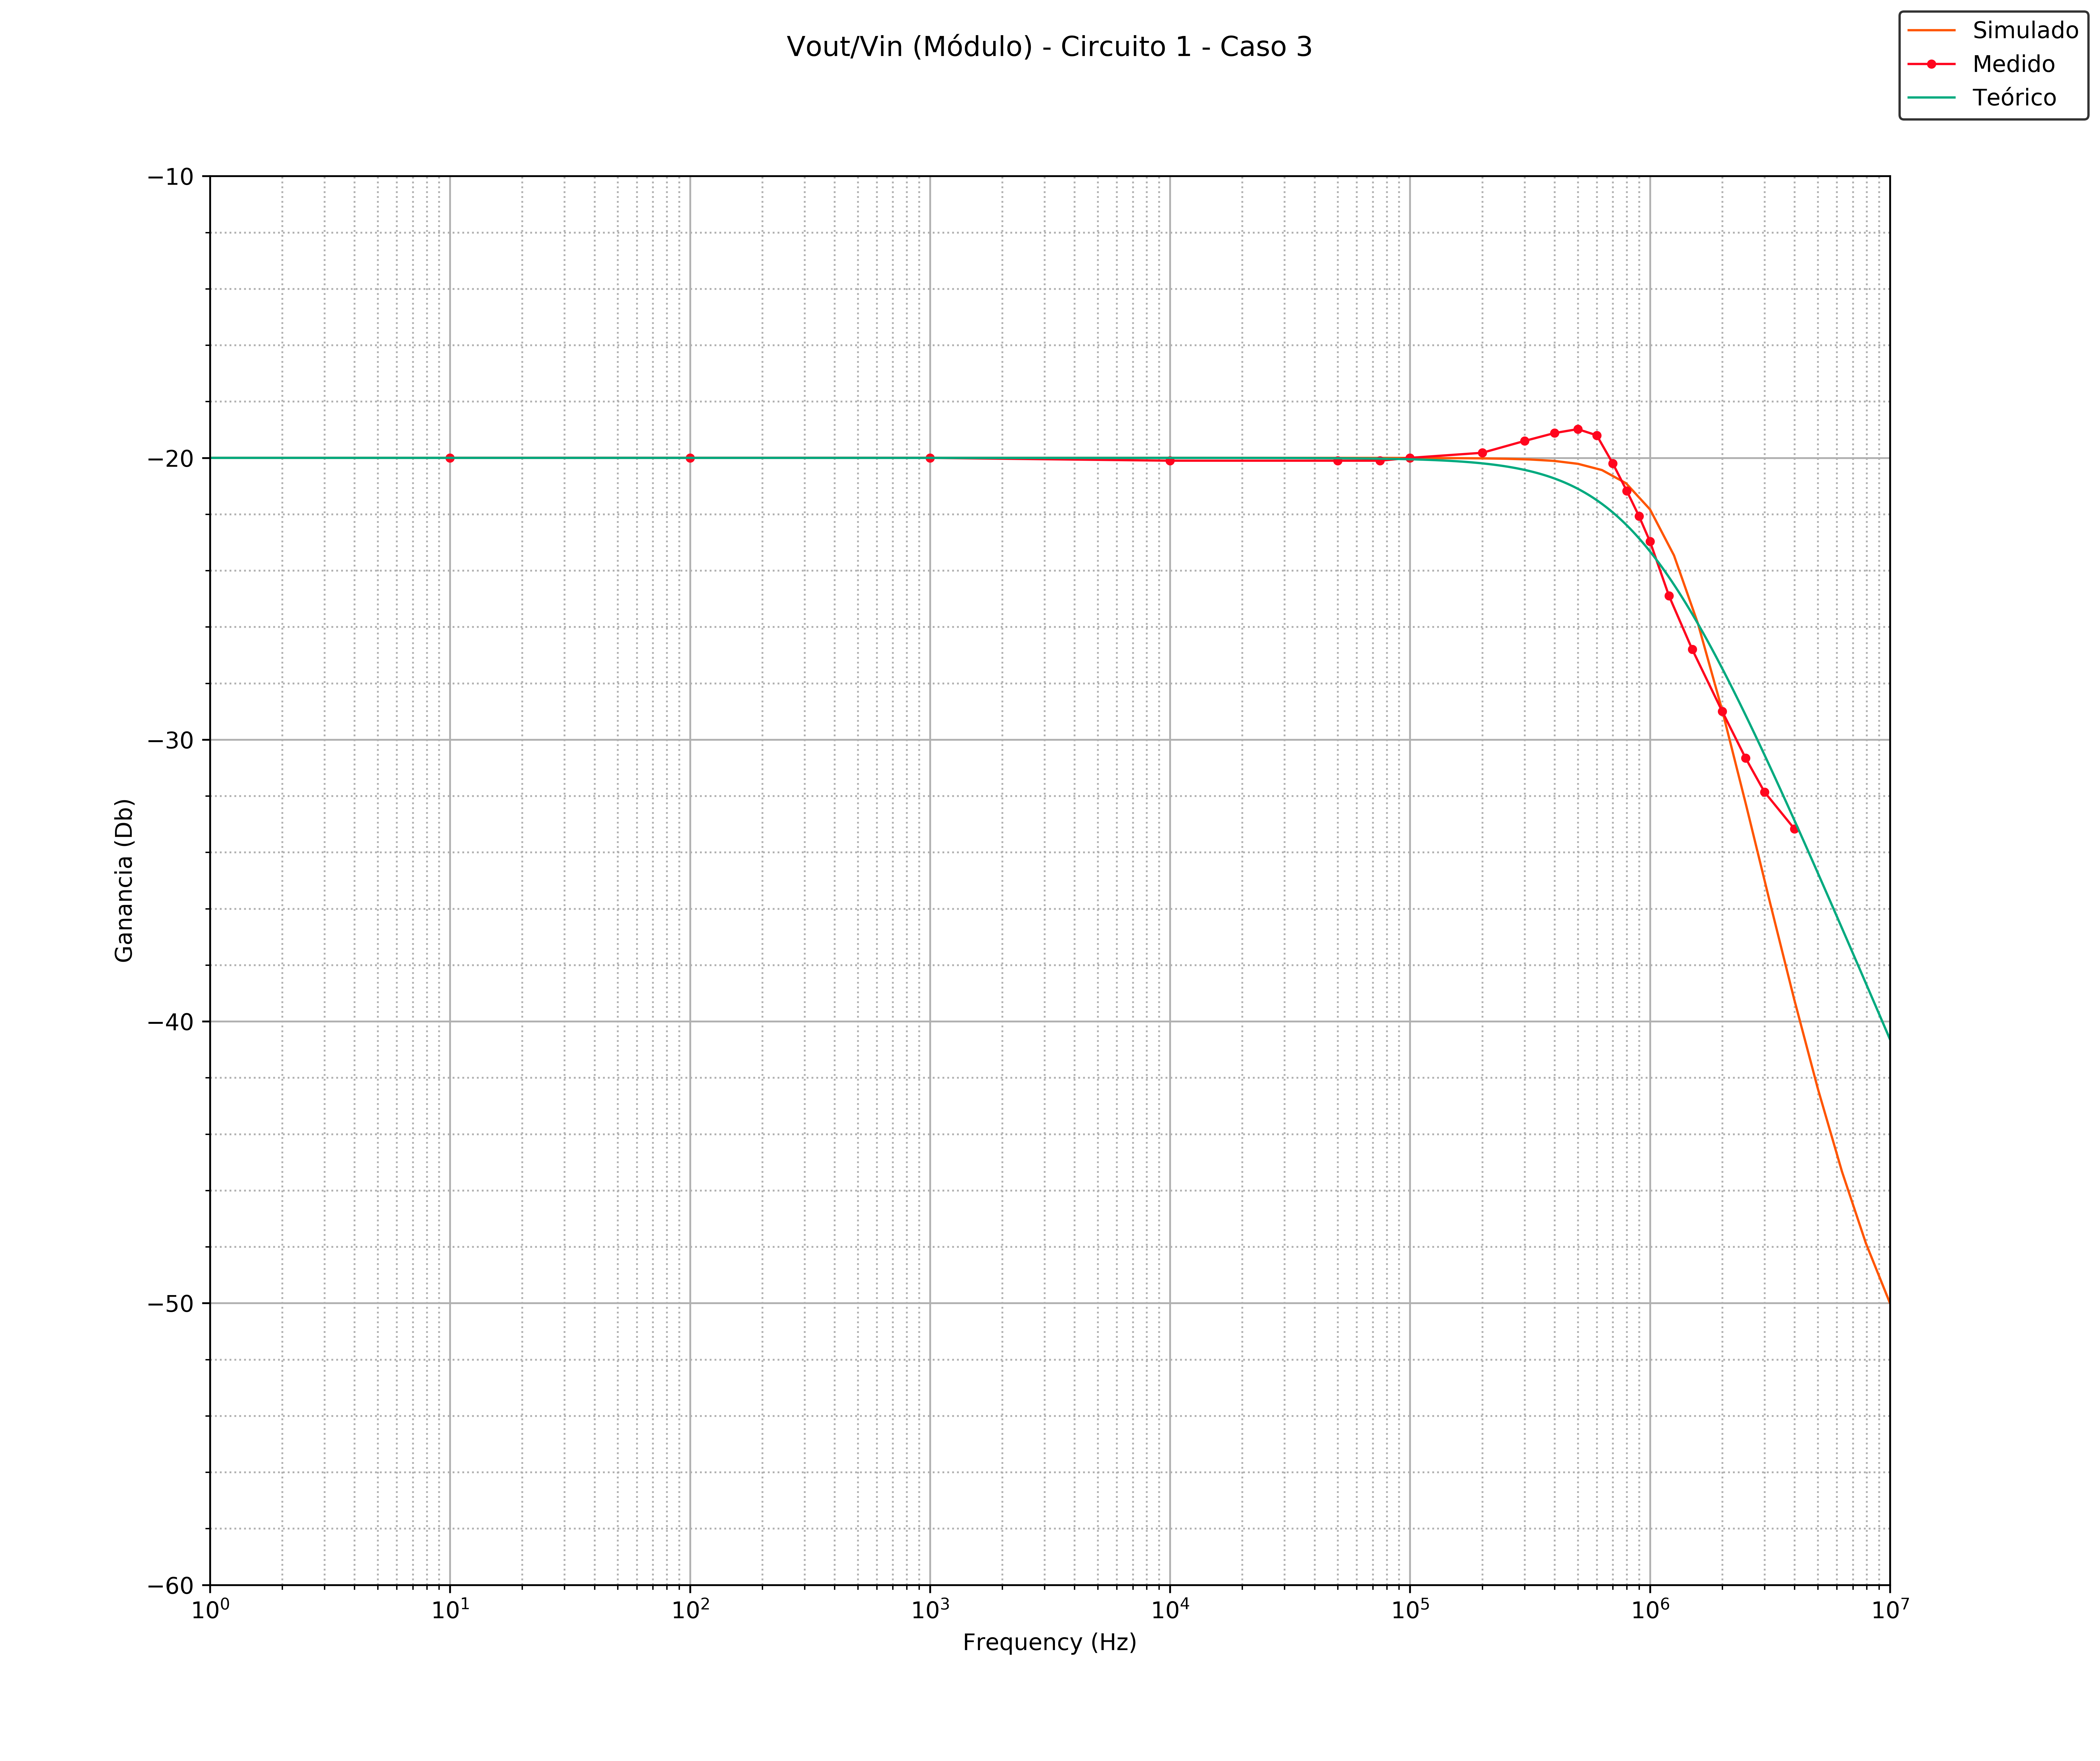
\includegraphics[width=10cm,height=10cm,keepaspectratio]{../EJ1/00GRAFICOS/c1c3/c1c3voviMod.png}
	\caption{Configuración inversora - Caso 3 - M\'odulo de$V_{out}/V_{in}$}	
	\label{c1c3voviM}
\end{figure}

\begin{figure}[H] %!ht
	\centering
	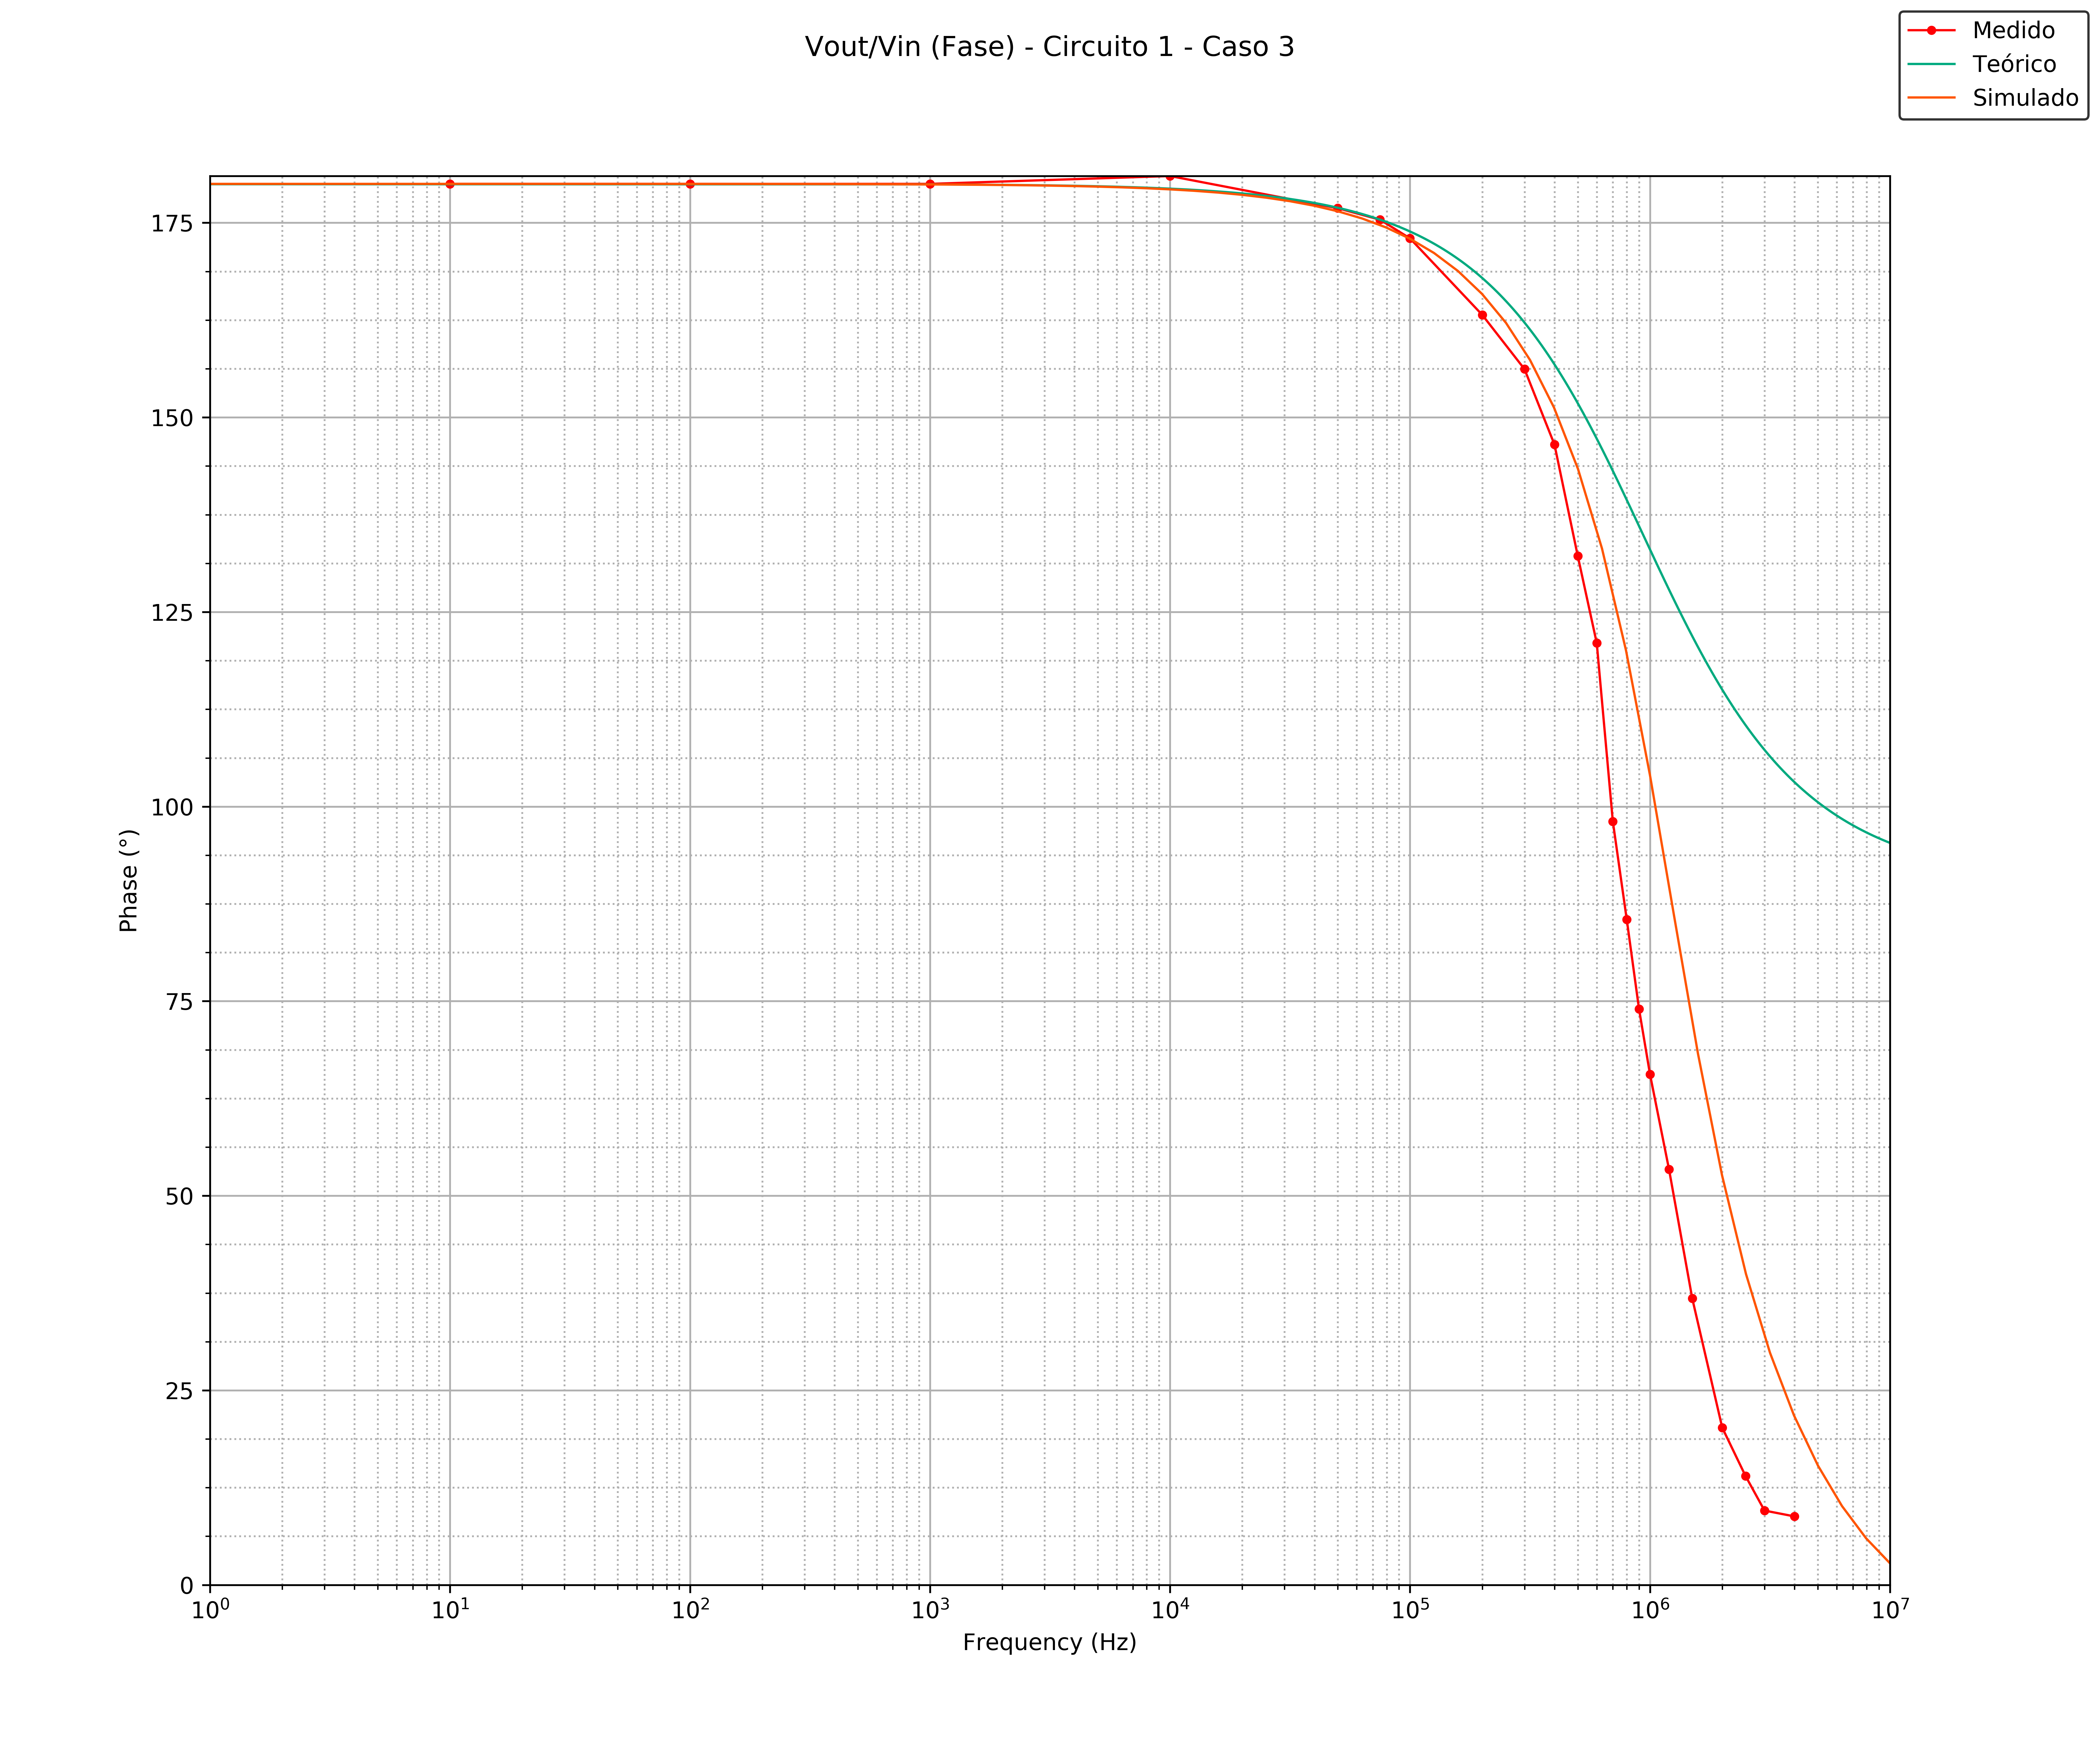
\includegraphics[width=10cm,height=10cm,keepaspectratio]{../EJ1/00GRAFICOS/c1c3/c1c3voviFASE.png}
	\caption{Configuración inversora - Fase de $V_{out}/V_{in}$}
	\label{c1c3voviP}
\end{figure}

\subsubsection{Impedancia de entrada del circuito} %%%%%


\subsubsection*{An\'alisis te\'orico} %%%%%%
Se hicieron distintos c\'alculos que permitieron obtener expresiones distintas para la impedancia de entrada del circuito.

Es importante mencionar que en primer lugar se consider\'o al amplificador operacional como ideal. Si bien las caracter\'isticas de dicha situaci\'on fueron mencionadas previamente, se considera relevante hacer unas breves aclaraciones para comprender el resultado de este an\'alisis. La impedancia entre los bornes de entrada del amplificador operacional fue, por lo tanto, tomada como infinita (circuito abierto); mientras que la impedancia interna a la salida del amplificador operacional fue considerada como cero (cable). Dado que en el caso ideal del amplificador operacional hay una masa virtual en $V^-$ y que la entrada $V^+$ est\'a f\'isicamente conectada a Tierra, la fuente interna que se encuentra en serie con la impedancia de salida vale cero ya que depende de la diferencia de tensi\'on entre $V^+$ y $V^-$. Entonces, partiendo de las ecuaciones \ref{ecsbase} y operando matem\'aticamente se obtiene la siguiente expresi\'on:
%PONER FORMULA ZIN TEORICA IDEAL!!!
%GRAFICAR Y PONER FORMULAS TEORICAS DE CASO IDEAL!!!!!!!!!!!!!!!
%hablar de las diferencias entre cada caso

Dado que luego se llevar\'ian a cabo mediciones para contrastar los resultados con el c\'alculo te\'orico, se decidi\'o buscar la expresi\'on correspondiente a la $Z_{in}$ que incluyera una punta del osciloscopio, es decir, se calcul\'o la impedancia que ser\'ia vista idealmente al utilizar el osciloscopio. Para esto, se le agreg\'o en paralelo el modelo equivalente a una punta X10 (la empleada) al resultado obtenido previamente de la $Z_{in}$. Dicho modelo consiste en una resistencia de $10M\Omega$ en paralelo con un capacitor de $12pF$. As\'i se obtuvo la siguiente expresi\'on:
%EXPRESION CON PUNTA ZIN
%FORMULA CON PUNTA ZIN PARA CADA UNO DE LOS 3 CASOS
%GRAFICOS COMPARATIVOS.

\subsubsection*{Mediciones y resultados obtenidos} %%%%%%
Para medir la impedancia de entrada del circuito en funci\'on de la frecuencia, deb\'iamos hacer el cociente $V_{in}/I_{in}$. Si bien se puede medir la tensi\'on de entrada al circuito de forma directa con el osciloscopio, no es tan sensillo obtener la corriente que entra al circuito, ya que el osciloscopio mide tensiones y no corrientes. Se busc\'o una resistencia $R_L$ cuyo valor comerical fuera lo m\'as parecido posible (igual o el primero mayor) al valor obtenido en el c\'alculo te\'rico para cada uno de los casos de resistencias. Se coloc\'o dicha resistencia en serie al generador, a la entrada del circuito. Luego se midi\'o la ca\'ida de tensi\'on sobre ella, ya que al dividirla por el valor de la $R_L$ colocada se obtendr\'ia la corriente de entrada al circuito $I_{in}$. El criterio de buscar una resistencia similar al valor calculado de $Z_{in}$ surge de que si se pusiese una resistencia muy chica, la diferencia entre las tensiones medidas sobre sus bornes ser\'ia muy chica (aumentando incertidumbre) y si se colocase una resistencia muy grande, la tensi\'on que caer\'ia ser\'ia mucho mayor a la que caer\'ia en el circuito, haciendo que la tensi\'on luego de la resistencia sea muy chica (se podr\'ia acercar al nivel de ruido) y que la diferencia de tensi\'on entre sus bornes tienda a la tensi\'on entregada por el generador. Por eso se consider\'o \'optimo que la resistencia tenga un valor similar al calculado de forma te\'orica y en caso de no conseguir el mismo valor, prefiri\'endose un valor mayor y no menor.

\begin{figure}[H] %!ht
	\centering
	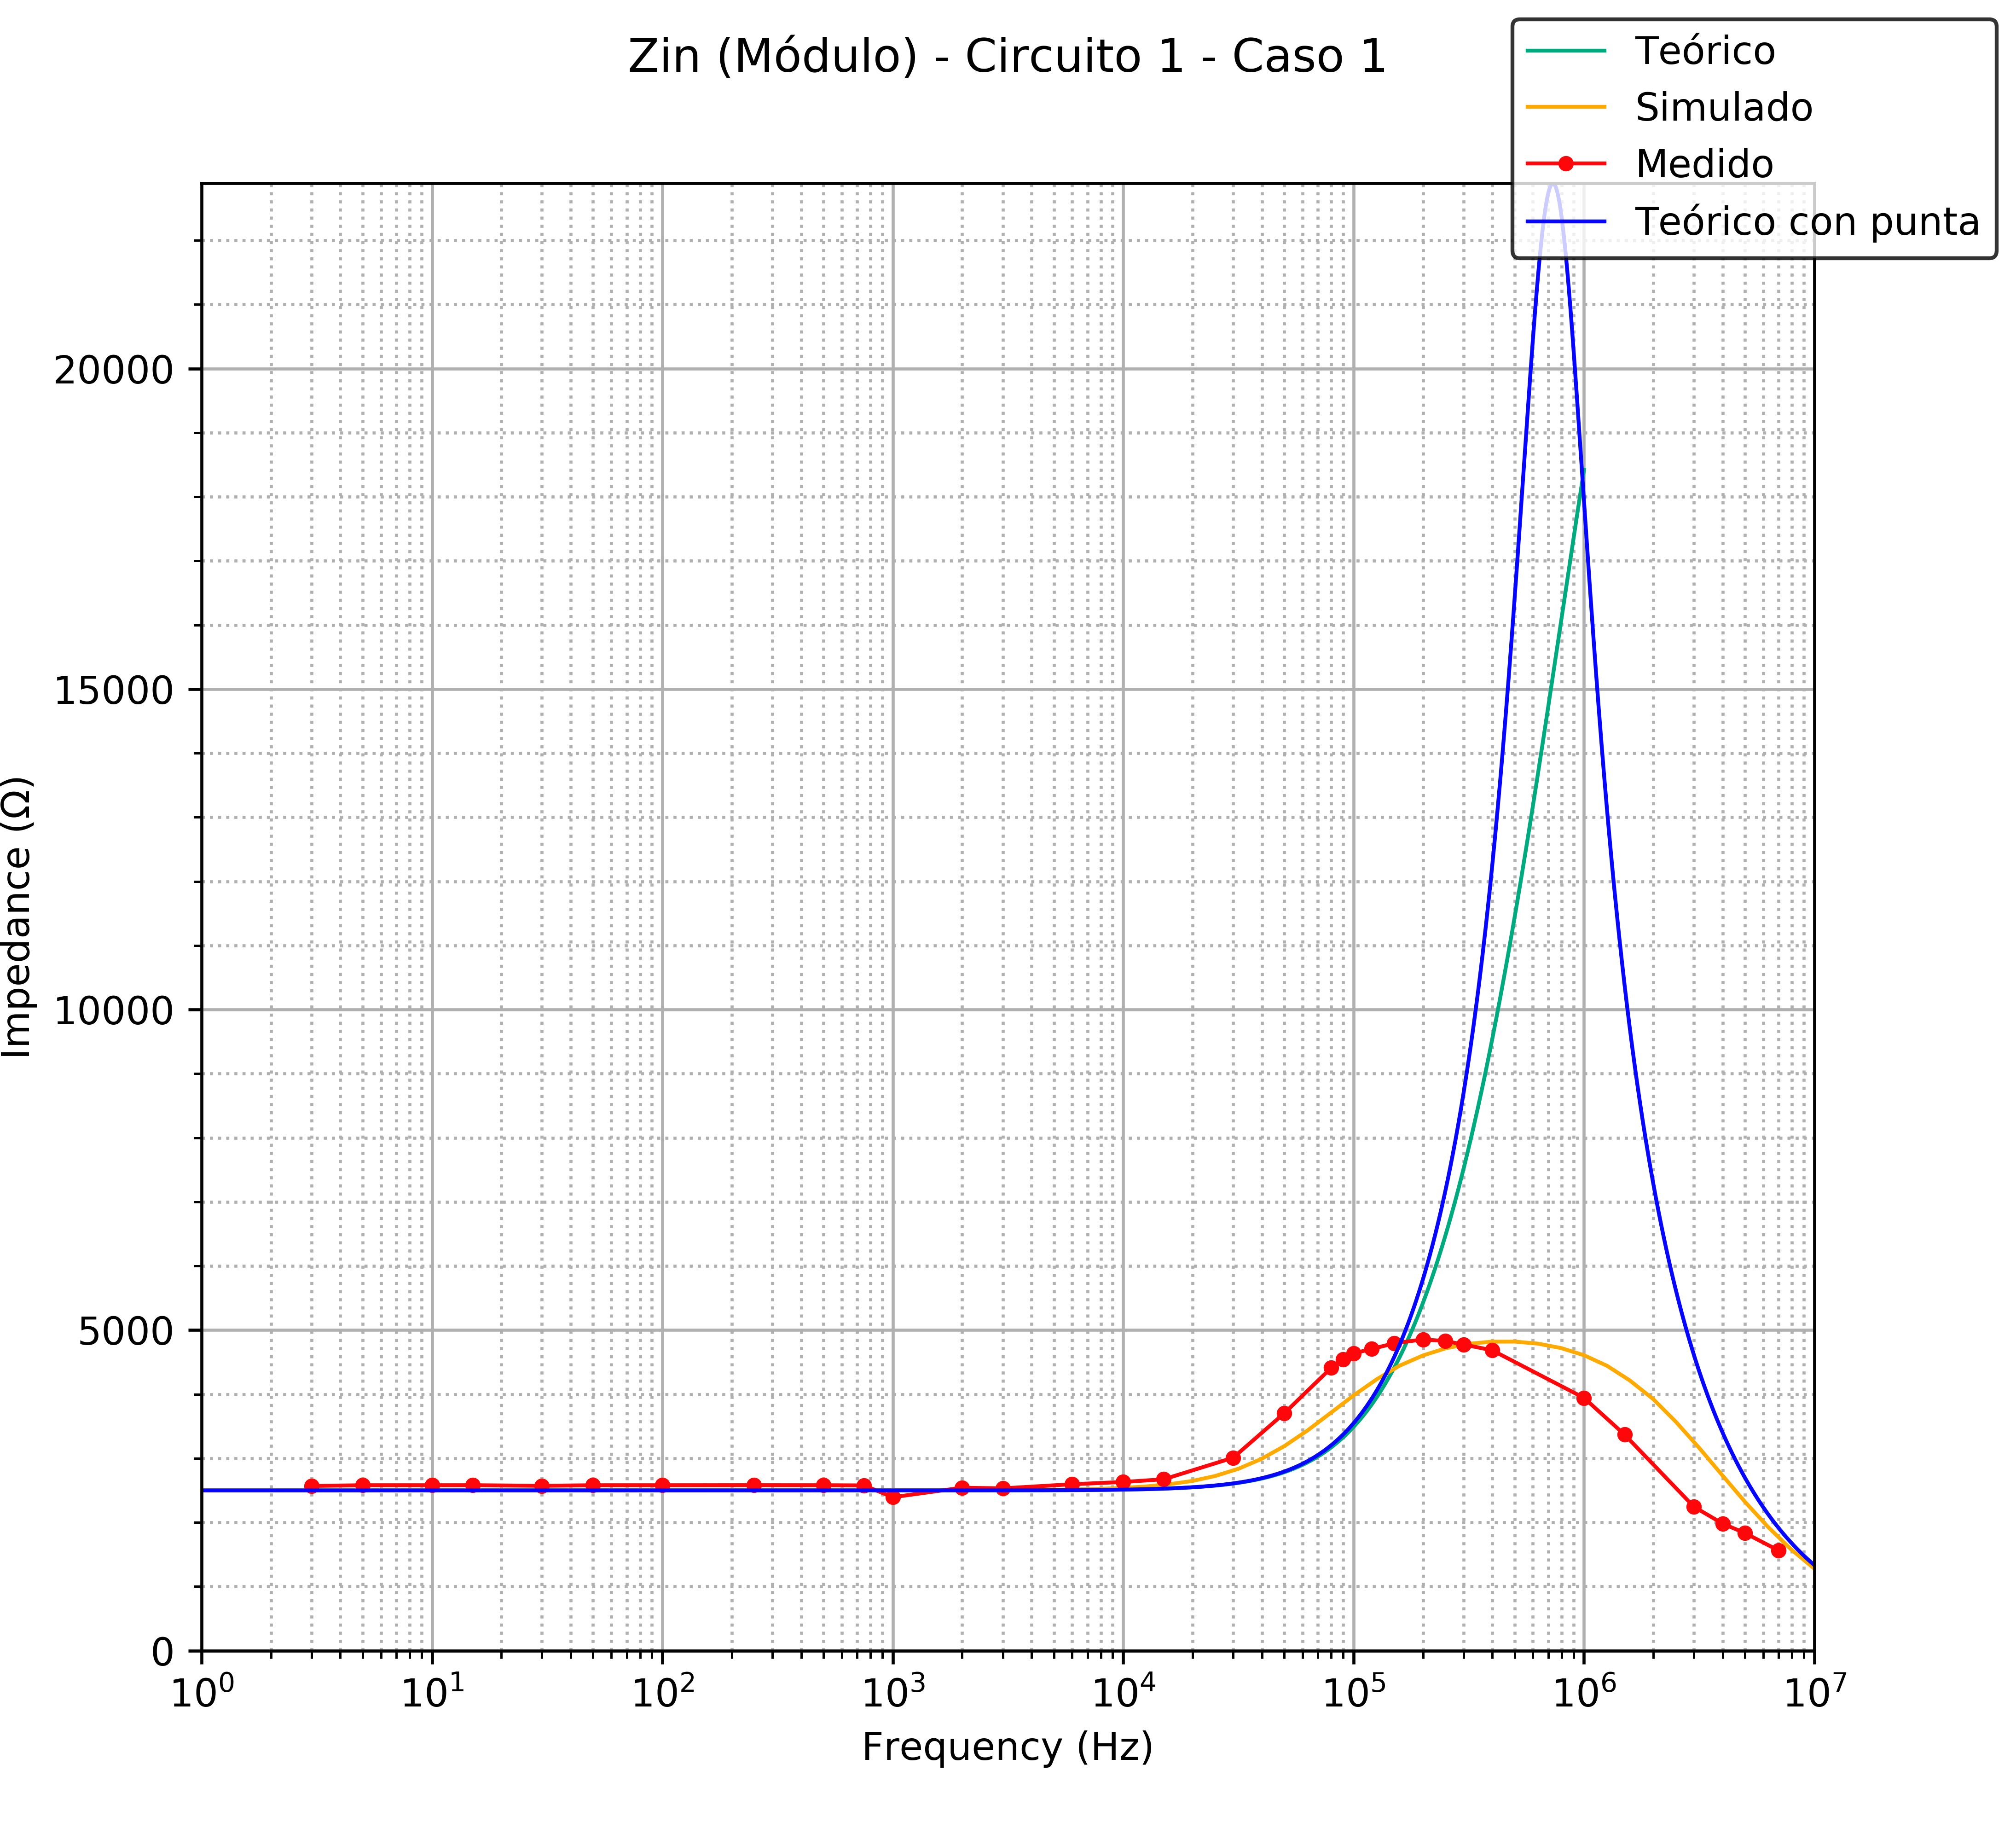
\includegraphics[width=10cm,height=10cm,keepaspectratio]{../EJ1/00GRAFICOS/c1c1/c1c1ZINpunta.png}
	\caption{Configuración inversora - Caso 1 - M\'odulo de $Z_{in}$}
	\label{c1c1zinM}
\end{figure}

\begin{figure}[H] %!ht
	\centering
	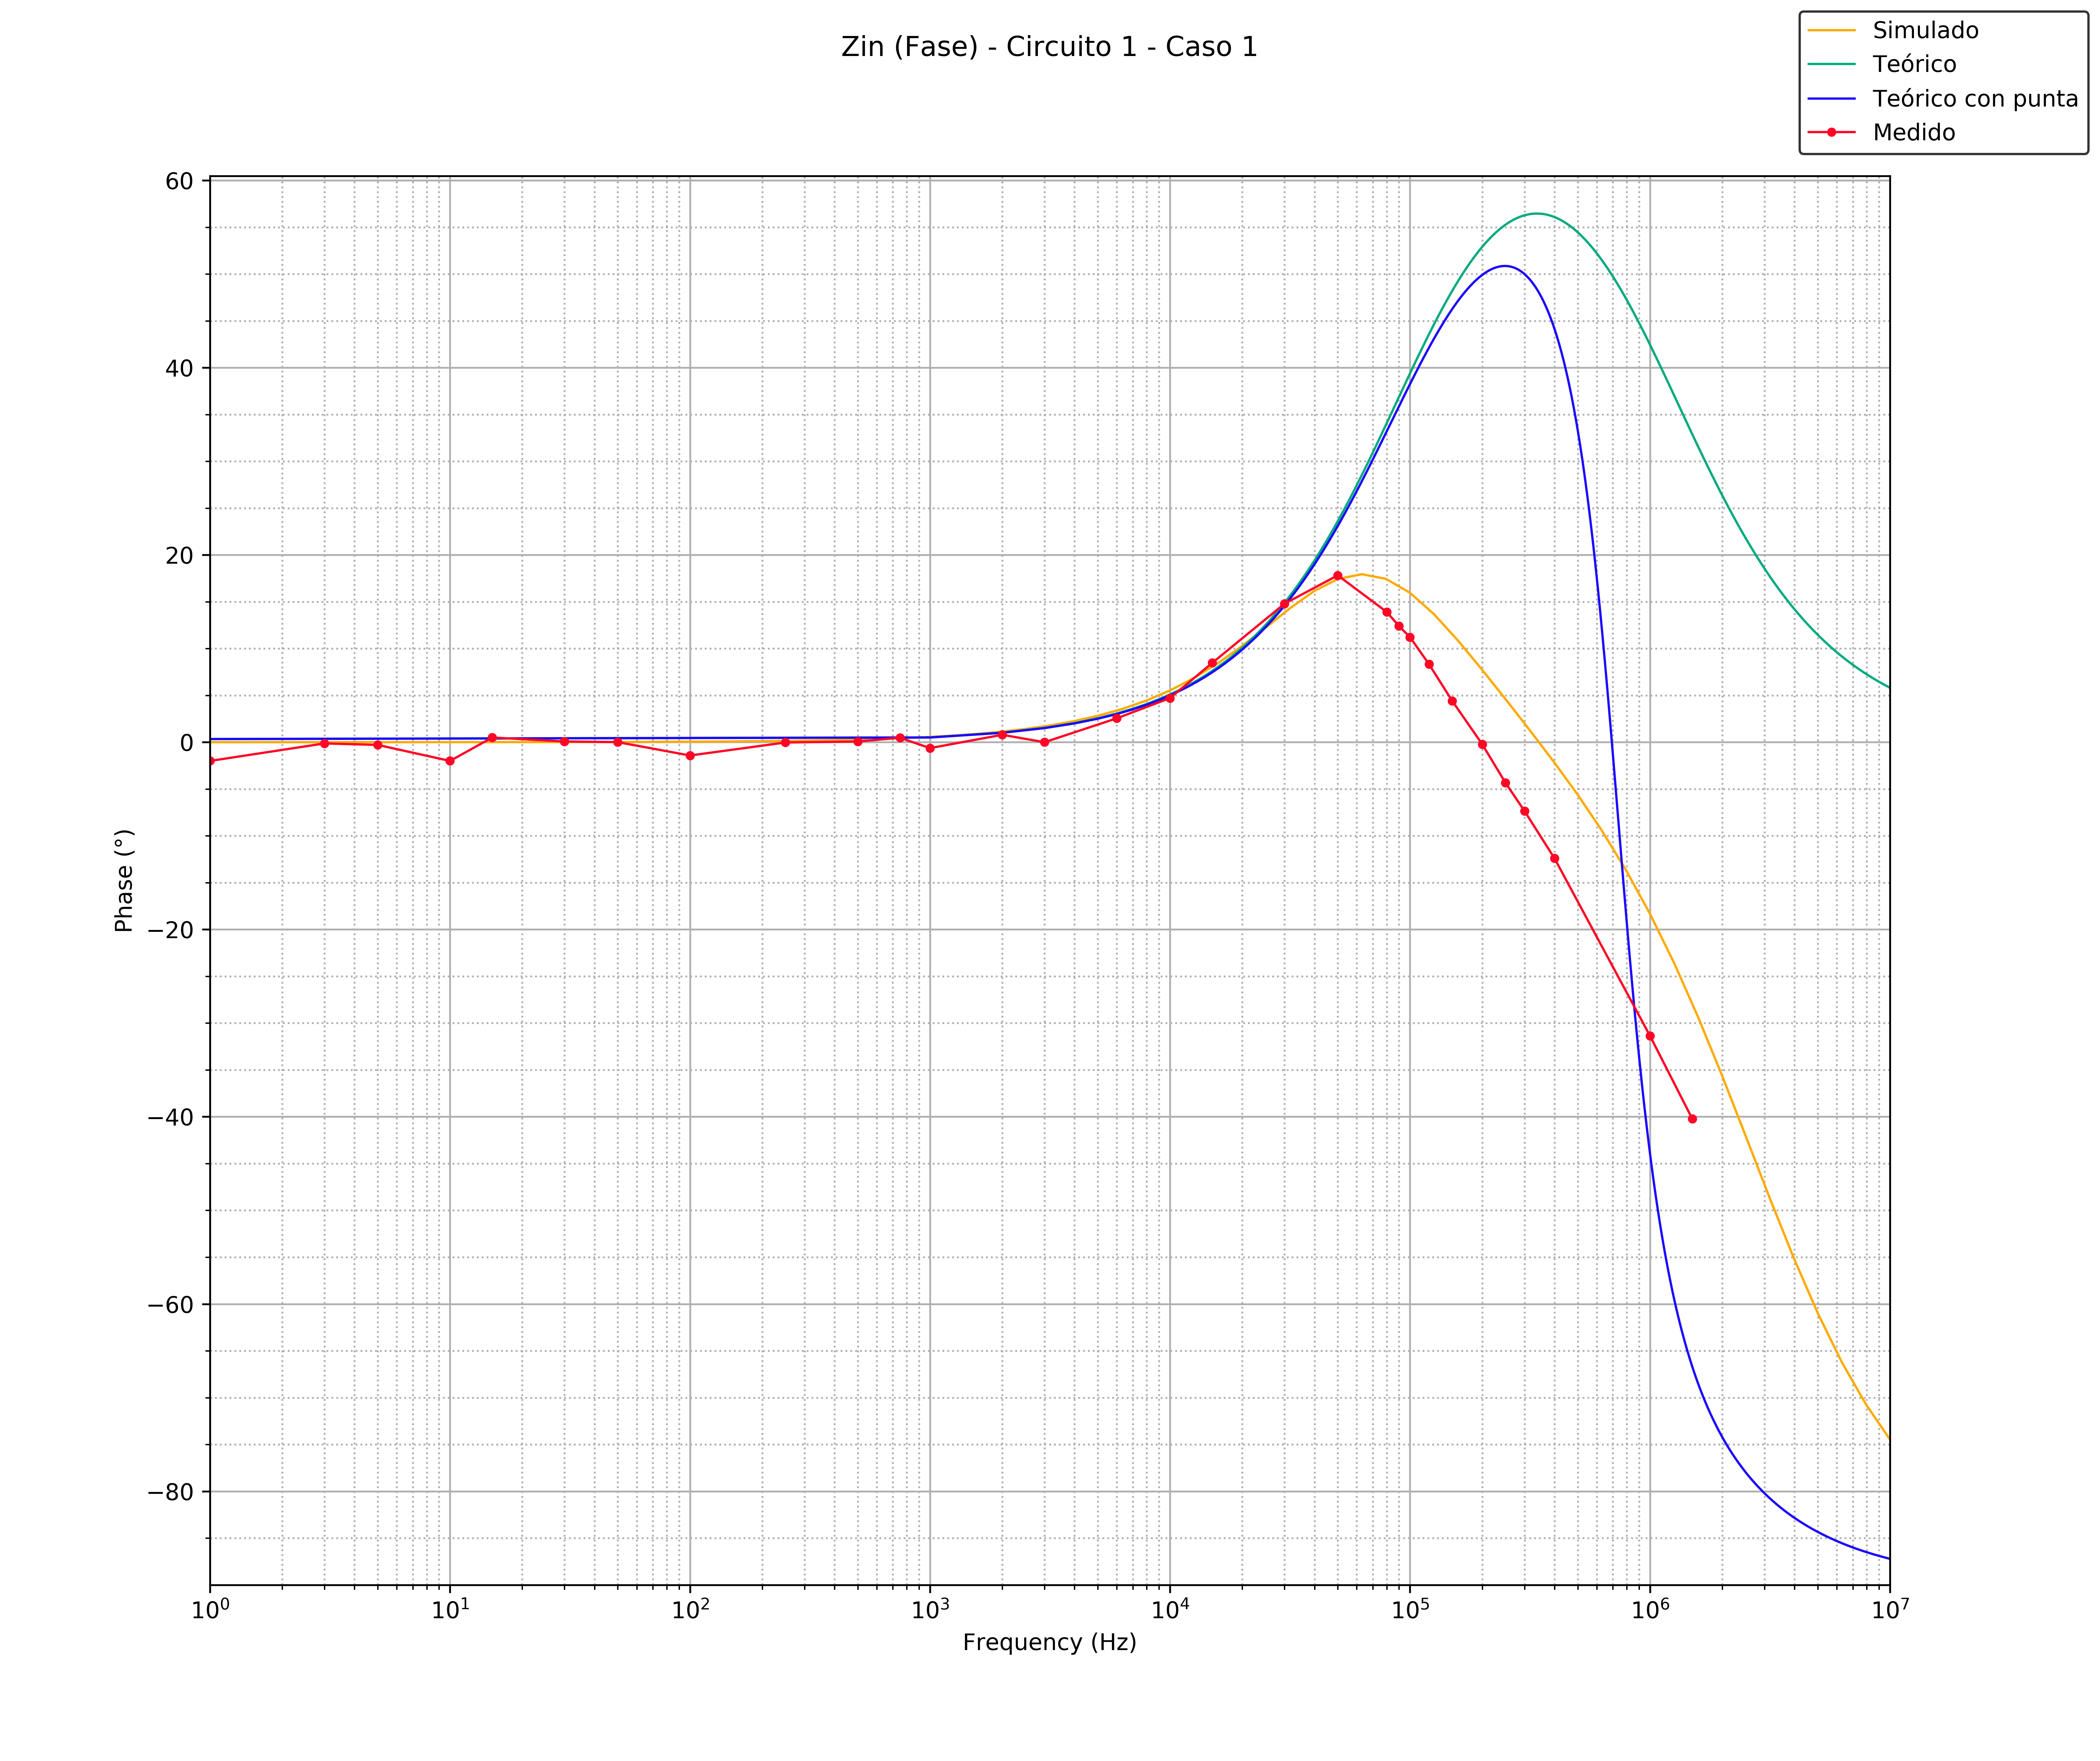
\includegraphics[width=10cm,height=10cm,keepaspectratio]{../EJ1/00GRAFICOS/c1c1/c1c1zinFASE.png}
	\caption{Configuración inversora - Caso 1 - Fase de $Z_{in}$ }
	\label{c1c1zinP}
\end{figure}

\begin{figure}[H] %!ht
	\centering
	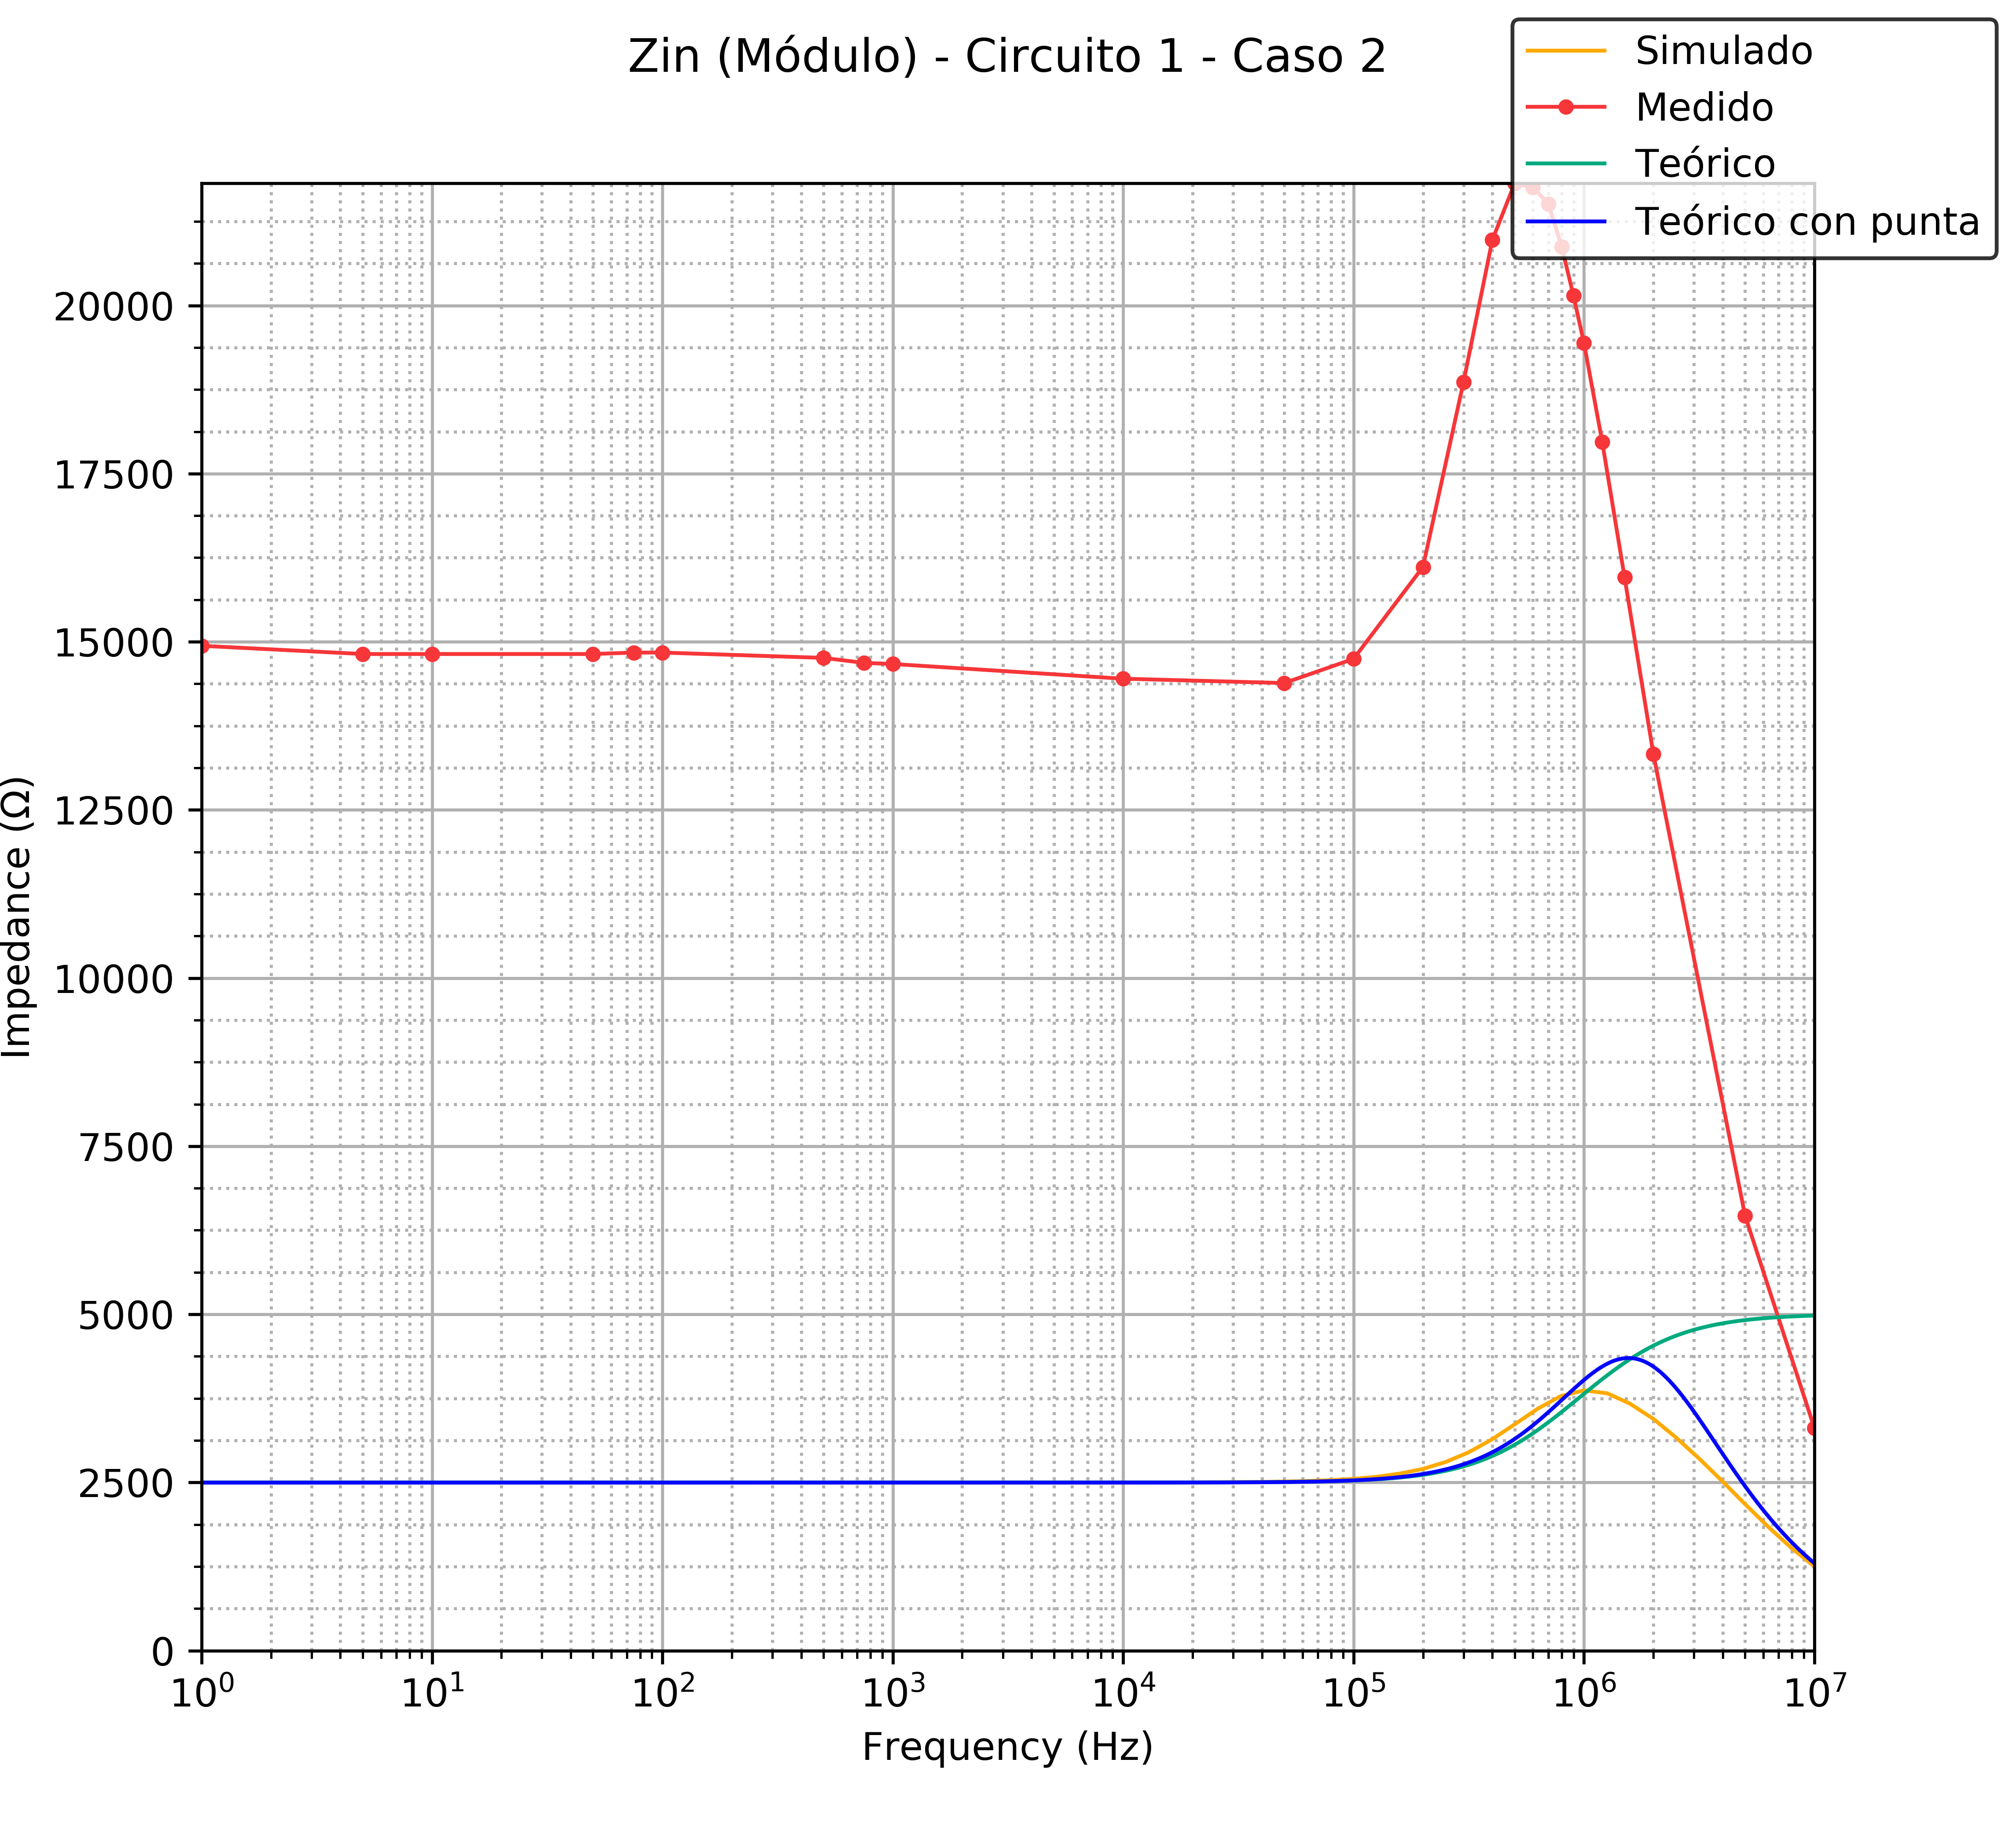
\includegraphics[width=10cm,height=10cm,keepaspectratio]{../EJ1/00GRAFICOS/c1c2/c1c2ZINpunta.png}
	\caption{Configuración inversora - Caso 2 - M\'odulo de $Z_{in}$}
	\label{c1c2zinM}
\end{figure}

\begin{figure}[H] %!ht
	\centering
	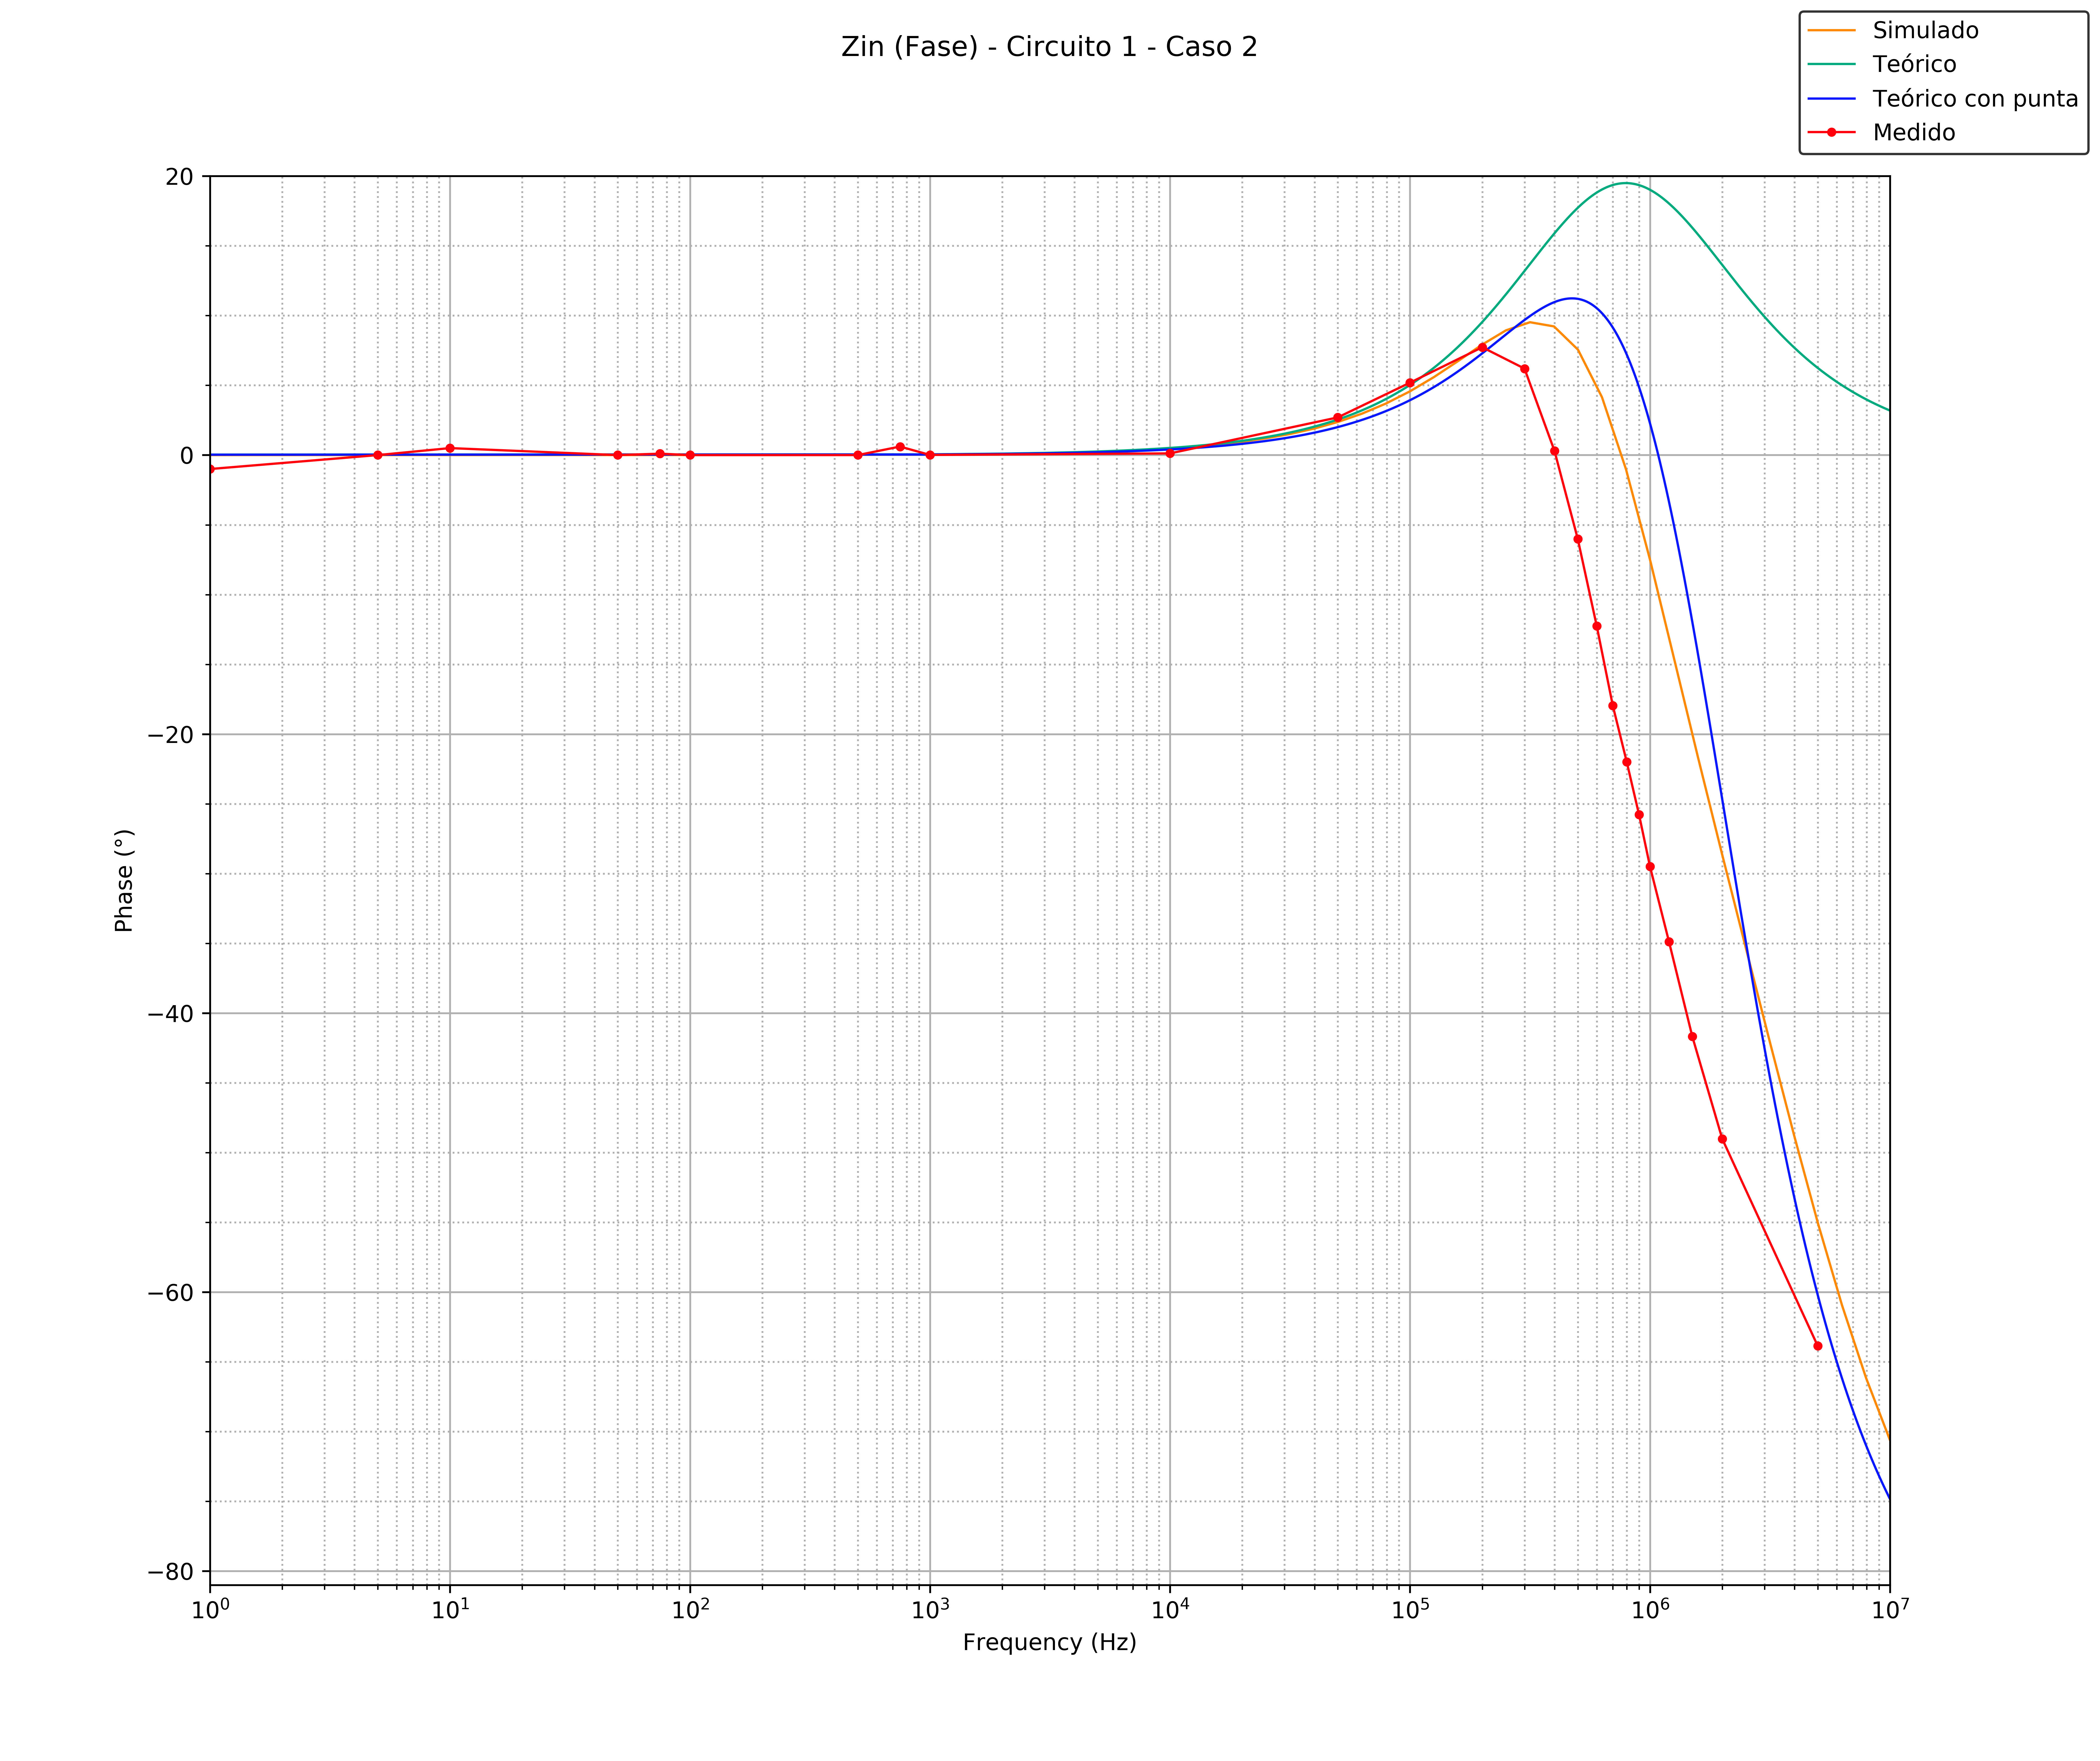
\includegraphics[width=10cm,height=10cm,keepaspectratio]{../EJ1/00GRAFICOS/c1c2/c1c2zinFASE.png}
	\caption{Configuración inversora - Caso 2 - Fase de $Z_{in}$}
	\label{c1c2zinP}
\end{figure}

\begin{figure}[H] %!ht
	\centering
	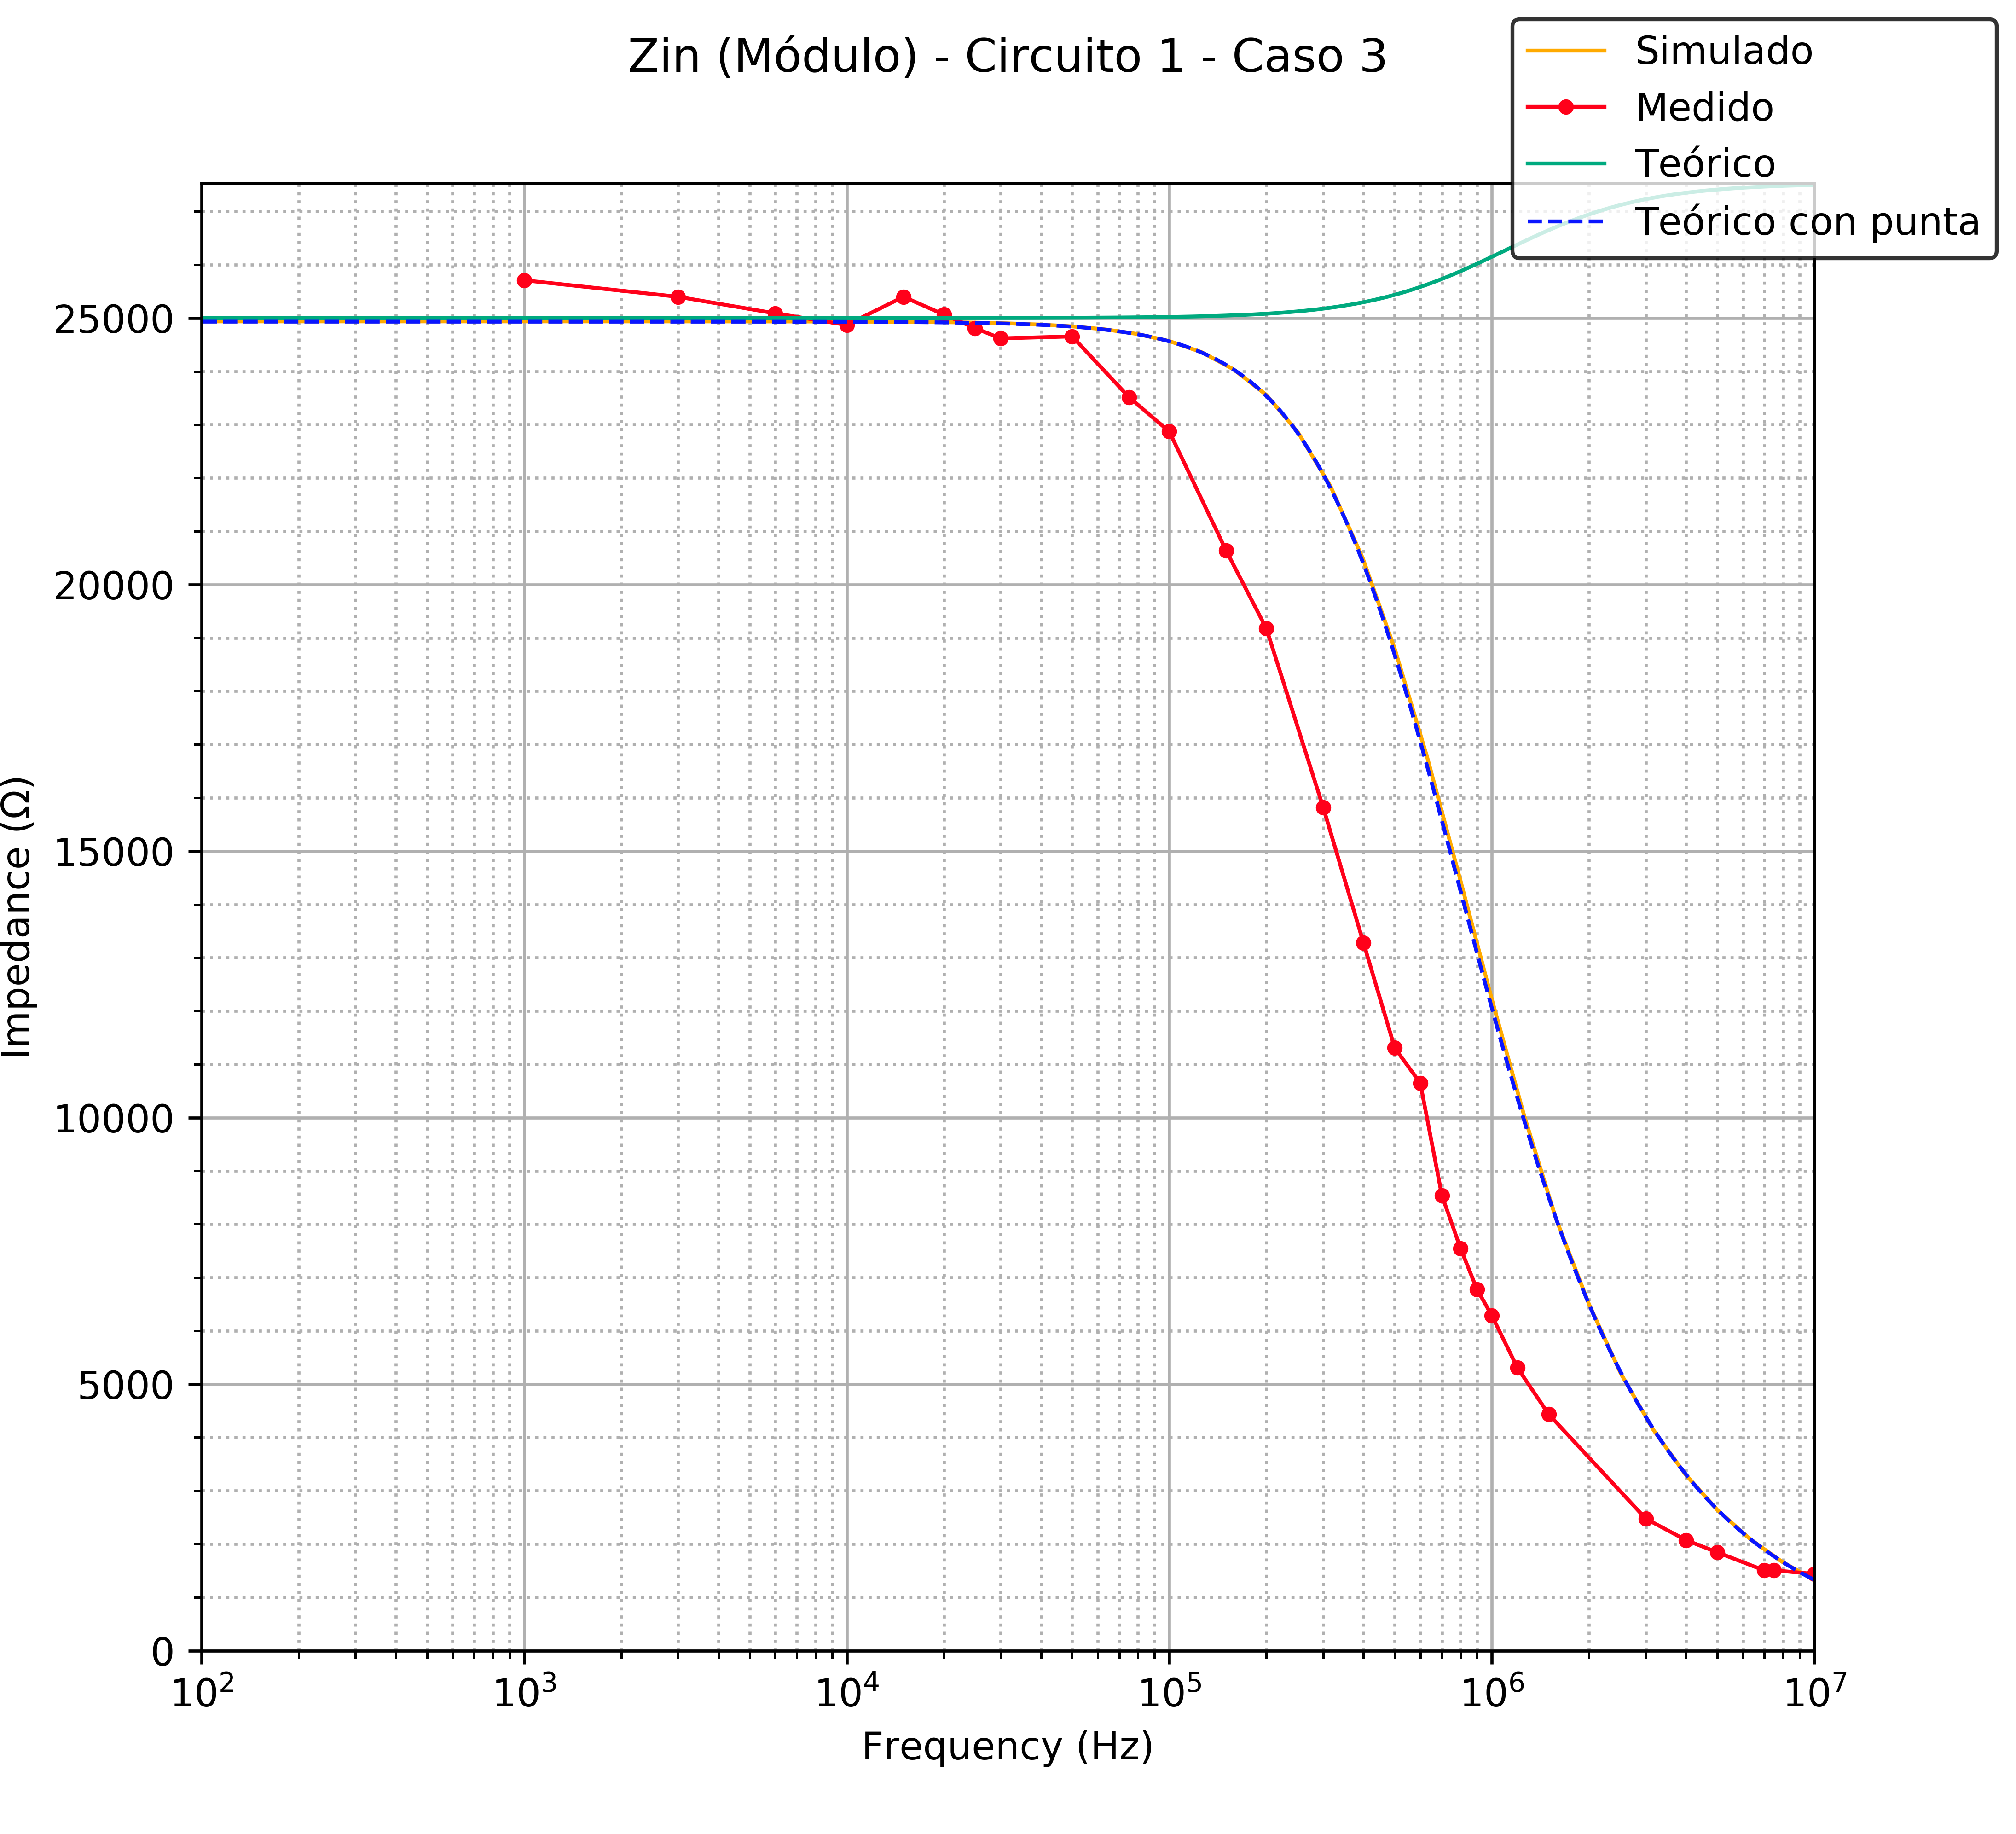
\includegraphics[width=10cm,height=10cm,keepaspectratio]{../EJ1/00GRAFICOS/c1c3/c1c3ZINpunta.png}
	\caption{Configuración inversora - Caso 3 - M\'odulo de $Z_{in}$}
	\label{c1c3zinM}
\end{figure}

\begin{figure}[H] %!ht
	\centering
	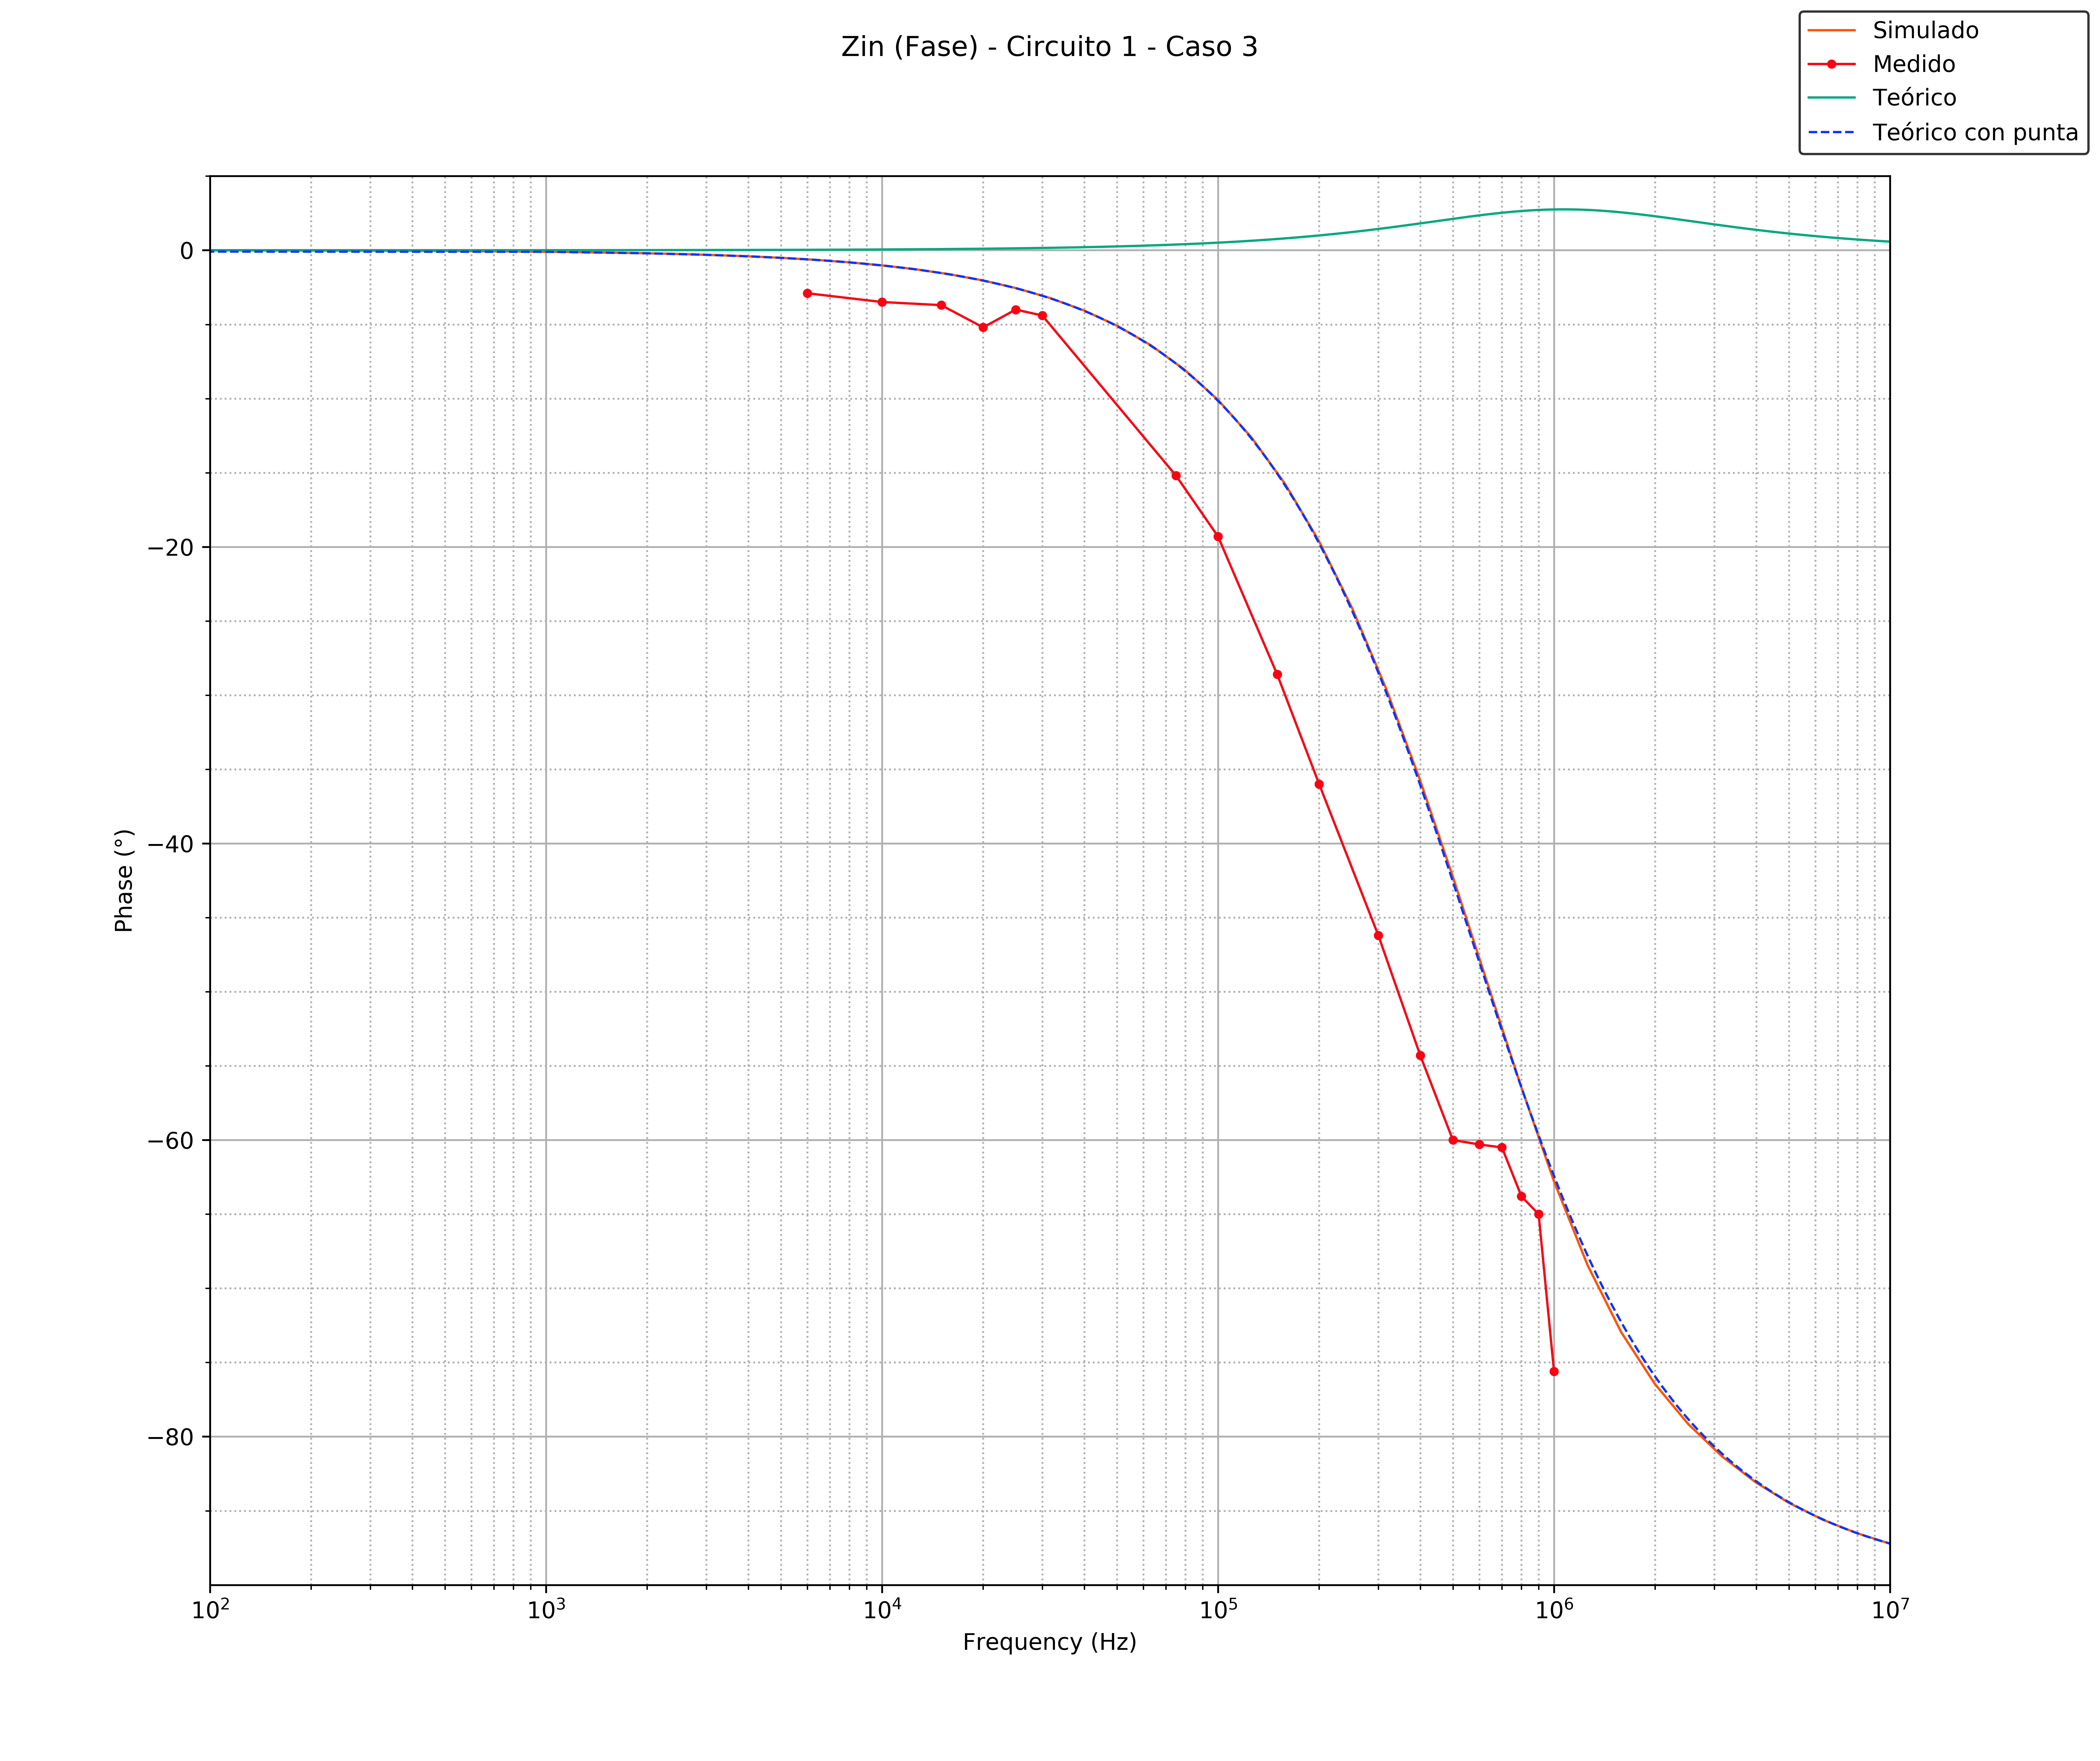
\includegraphics[width=10cm,height=10cm,keepaspectratio]{../EJ1/00GRAFICOS/c1c3/c1c3zinFASE.png}
	\caption{Configuración inversora - Caso 3 - Fase de $Z_{in}$}
	\label{c1c3zinP}
\end{figure}

\subsubsection{DC Sweep desde $-V_{CC}$ hasta $V_{CC}$}
%Buscar valor maximo en hoja de datos vcc aprox 17 creo.BUSCAR voutMAX!!!
Dado que se nos pidi\'o alimentar al amplificador operacional con $V_{CC} = \pm 15V$, un DC Sweep desde $-V_{CC}$ hasta $V_{CC}$ requerir\'ia $30V_{pp}$ del generador de se\~nales. Una limitaci\'on de los generadores del laboratorio es que alcanzan un m\'aximo de $20V_{pp}$, por lo que no podr\'iamos llevar a cabo las mediciones generando una rampa en el rango de tesniones mencionado. La desici\'on tomada para lograr lo pedido fue, en el dise\~no del circuito, agregarle una etapa previa de amplificaci\'on utilizando otro amplificador operacional. 
El amplificador operacional no permite amplificar mas de un valor determinado, y por lo tanto no hay forma de llegar exactamente a -15V y a 15V a la entrada del circuito ya que su tensi\'on de entrada es la salida del amplificador operacional empleado en la etapa previa de amplificaci\'on de la se\~nal del generador.
%BUSCAR VALORES!!!!!!

\subsubsection{Presencia de la resistencia $R_4$}
%HACER

\subsubsection{Ausencia de la resistencia $R_3$}
%HACER

\subsubsection{Fen\'omenos que afectan al comportamiento del circuito} %VER SI DEJAR PARA C/CASO O AL FINAL, for BOTH, o al ppio introductoriamente
	\subsubsection*{Efecto de slew rate (SR)}
	\subsubsection*{Distorsi\'on de cruce por cero (Cross-Over Distortion)}
	\subsubsection*{Gain Bandwidth Product (GBP)}

\subsubsection{Condiciones de comportamiento lineal del circuito}
%HACER


%%%%%%%%%%%%%%%%%%%%%%%%%%%%%%%%%%%%%%%%%%%%%%%%%%%
%%%%%%%%%%%%%%%%%% CIRCUITO 2 %%%%%%%%%%%%%%%%%%%%%%
%%%%%%%%%%%%%%%%%%%%%%%%%%%%%%%%%%%%%%%%%%%%%%%%%%%
\subsection{Configuraci\'on no inversora}

\subsubsection{Respuesta en frecuencia del circuito} %%%%%%
\subsubsection*{An\'alisis te\'orico} %%%%%%

\begin{figure}[H] %!ht
\centering
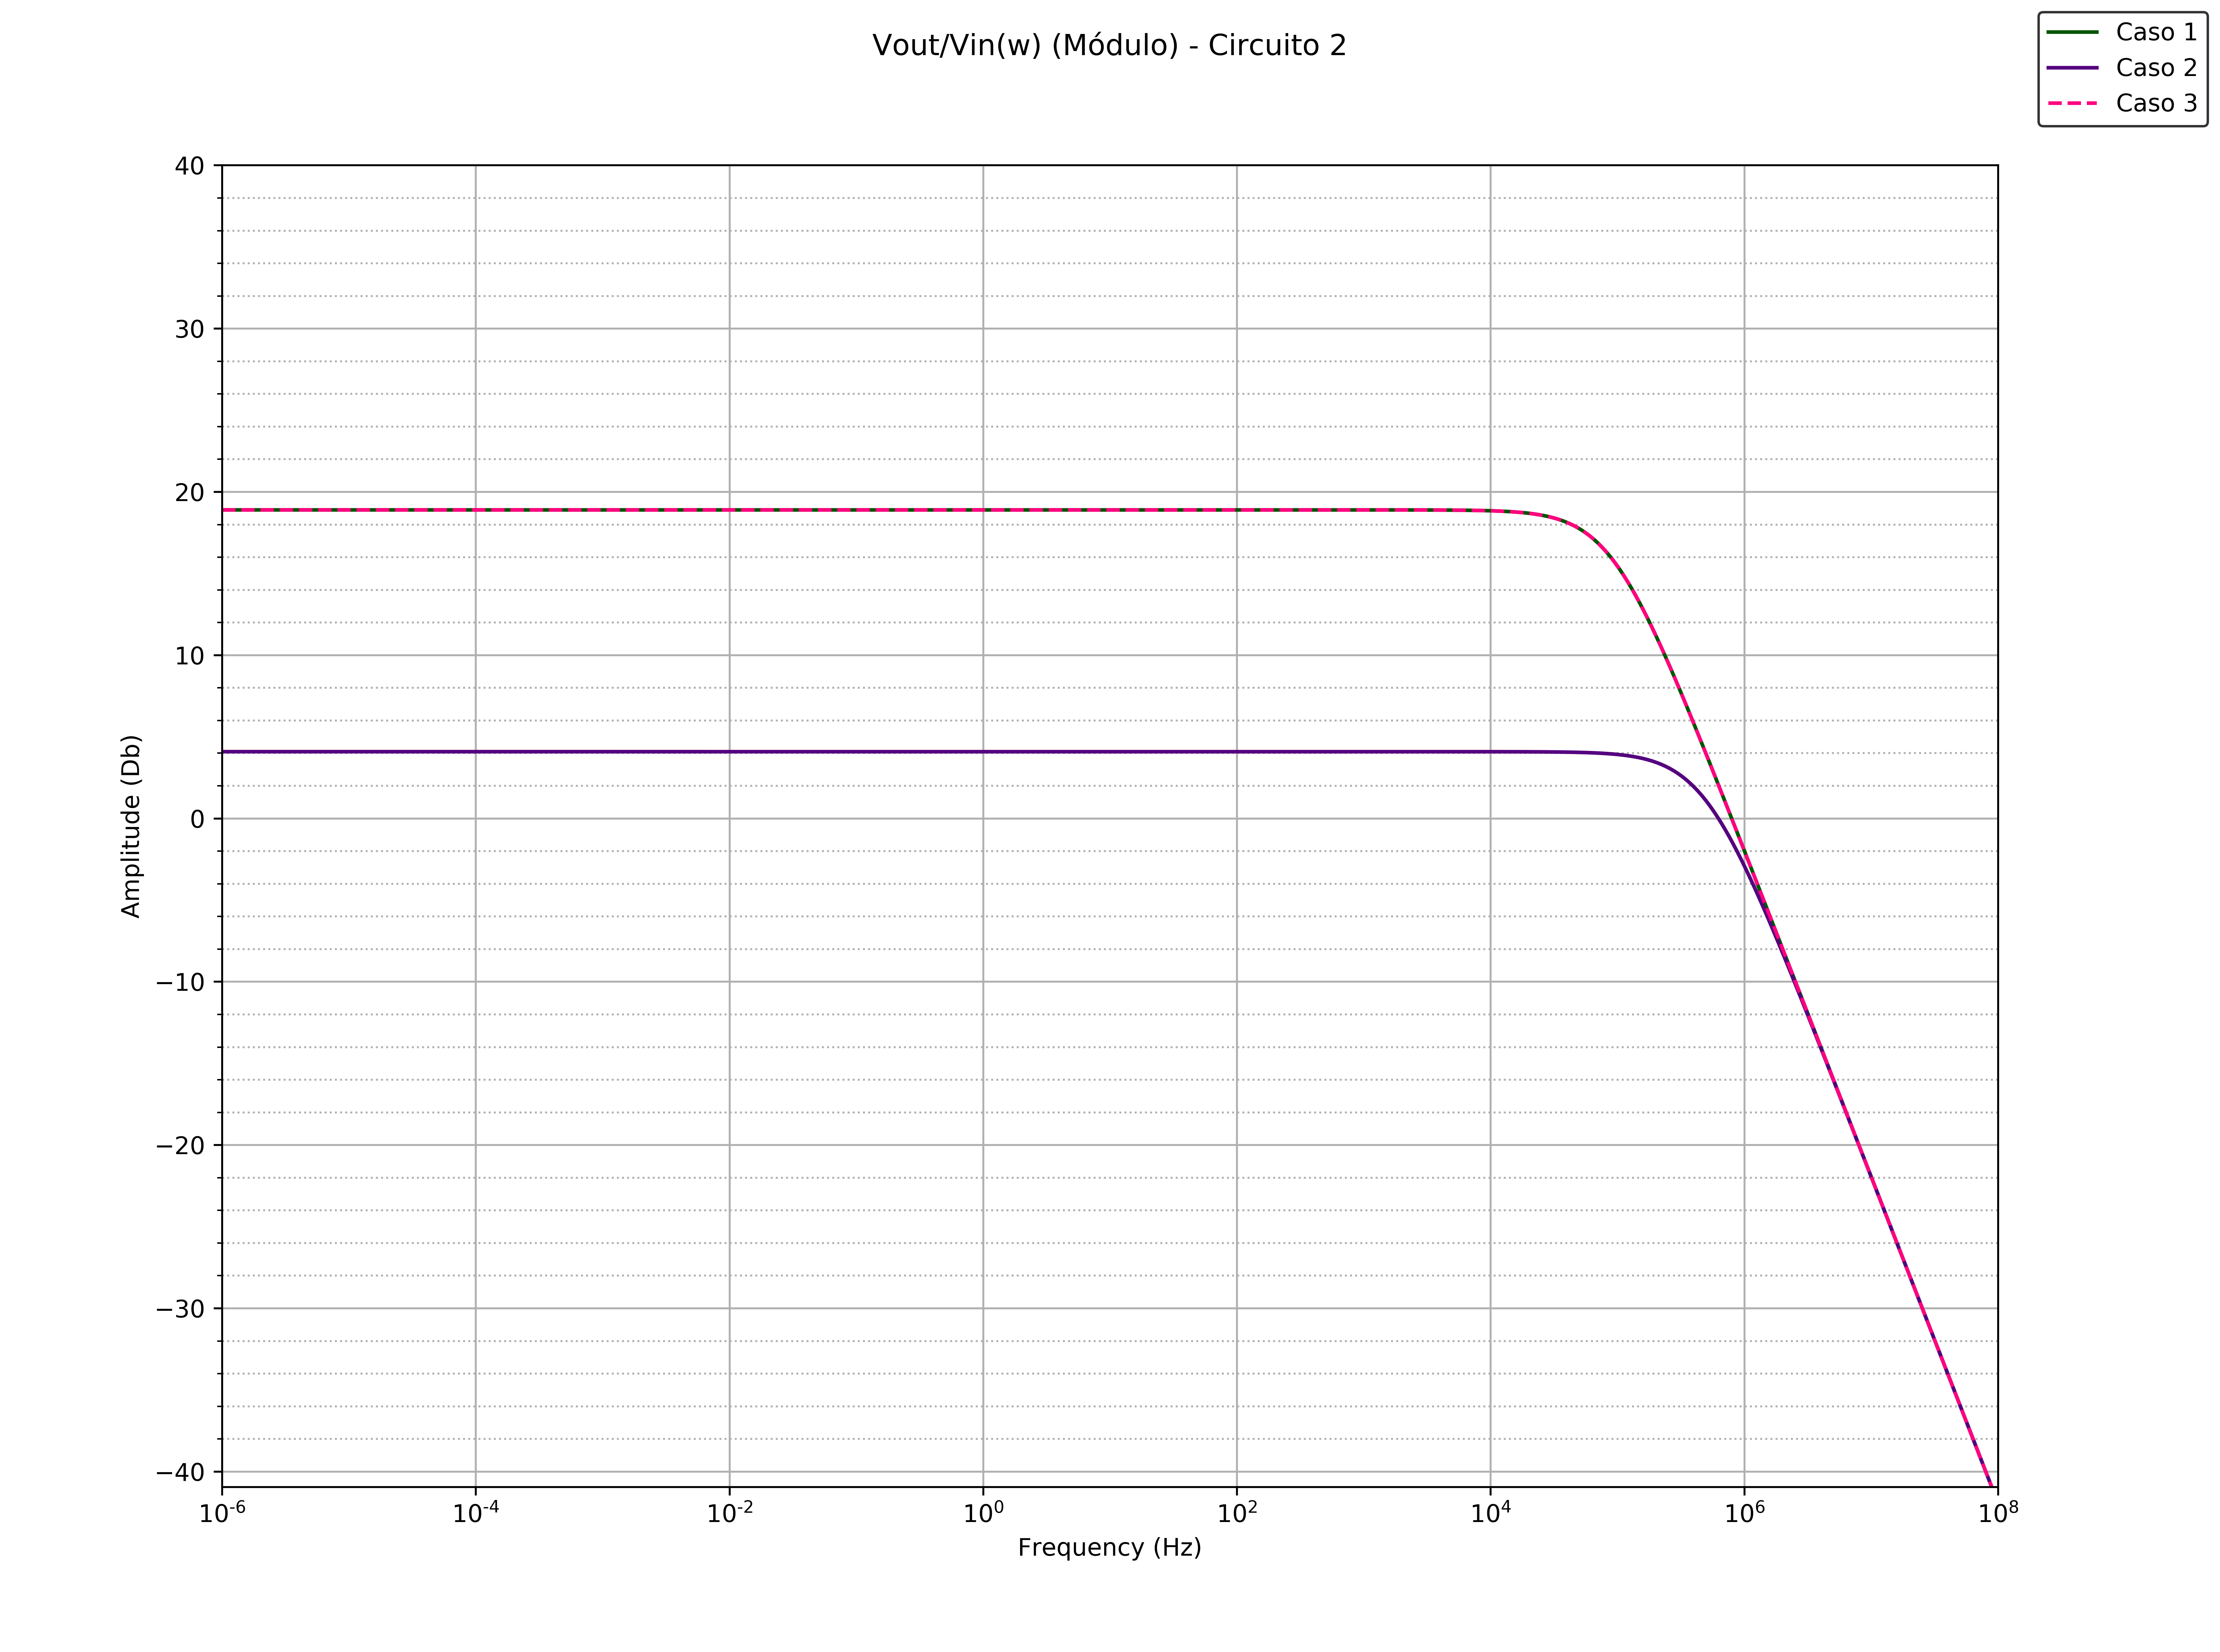
\includegraphics[width=10cm,height=10cm,keepaspectratio]{../EJ1/00GRAFICOS/teoricos/circ2voviw.png}
\caption{Configuración no inversora - Comparaci\'on te\'orica del m\'odulo de$V_{out}/V_{in}$ de los tres casos.}
\label{c2voviTeoMod}
\end{figure}

\begin{figure}[H] %!ht
\centering
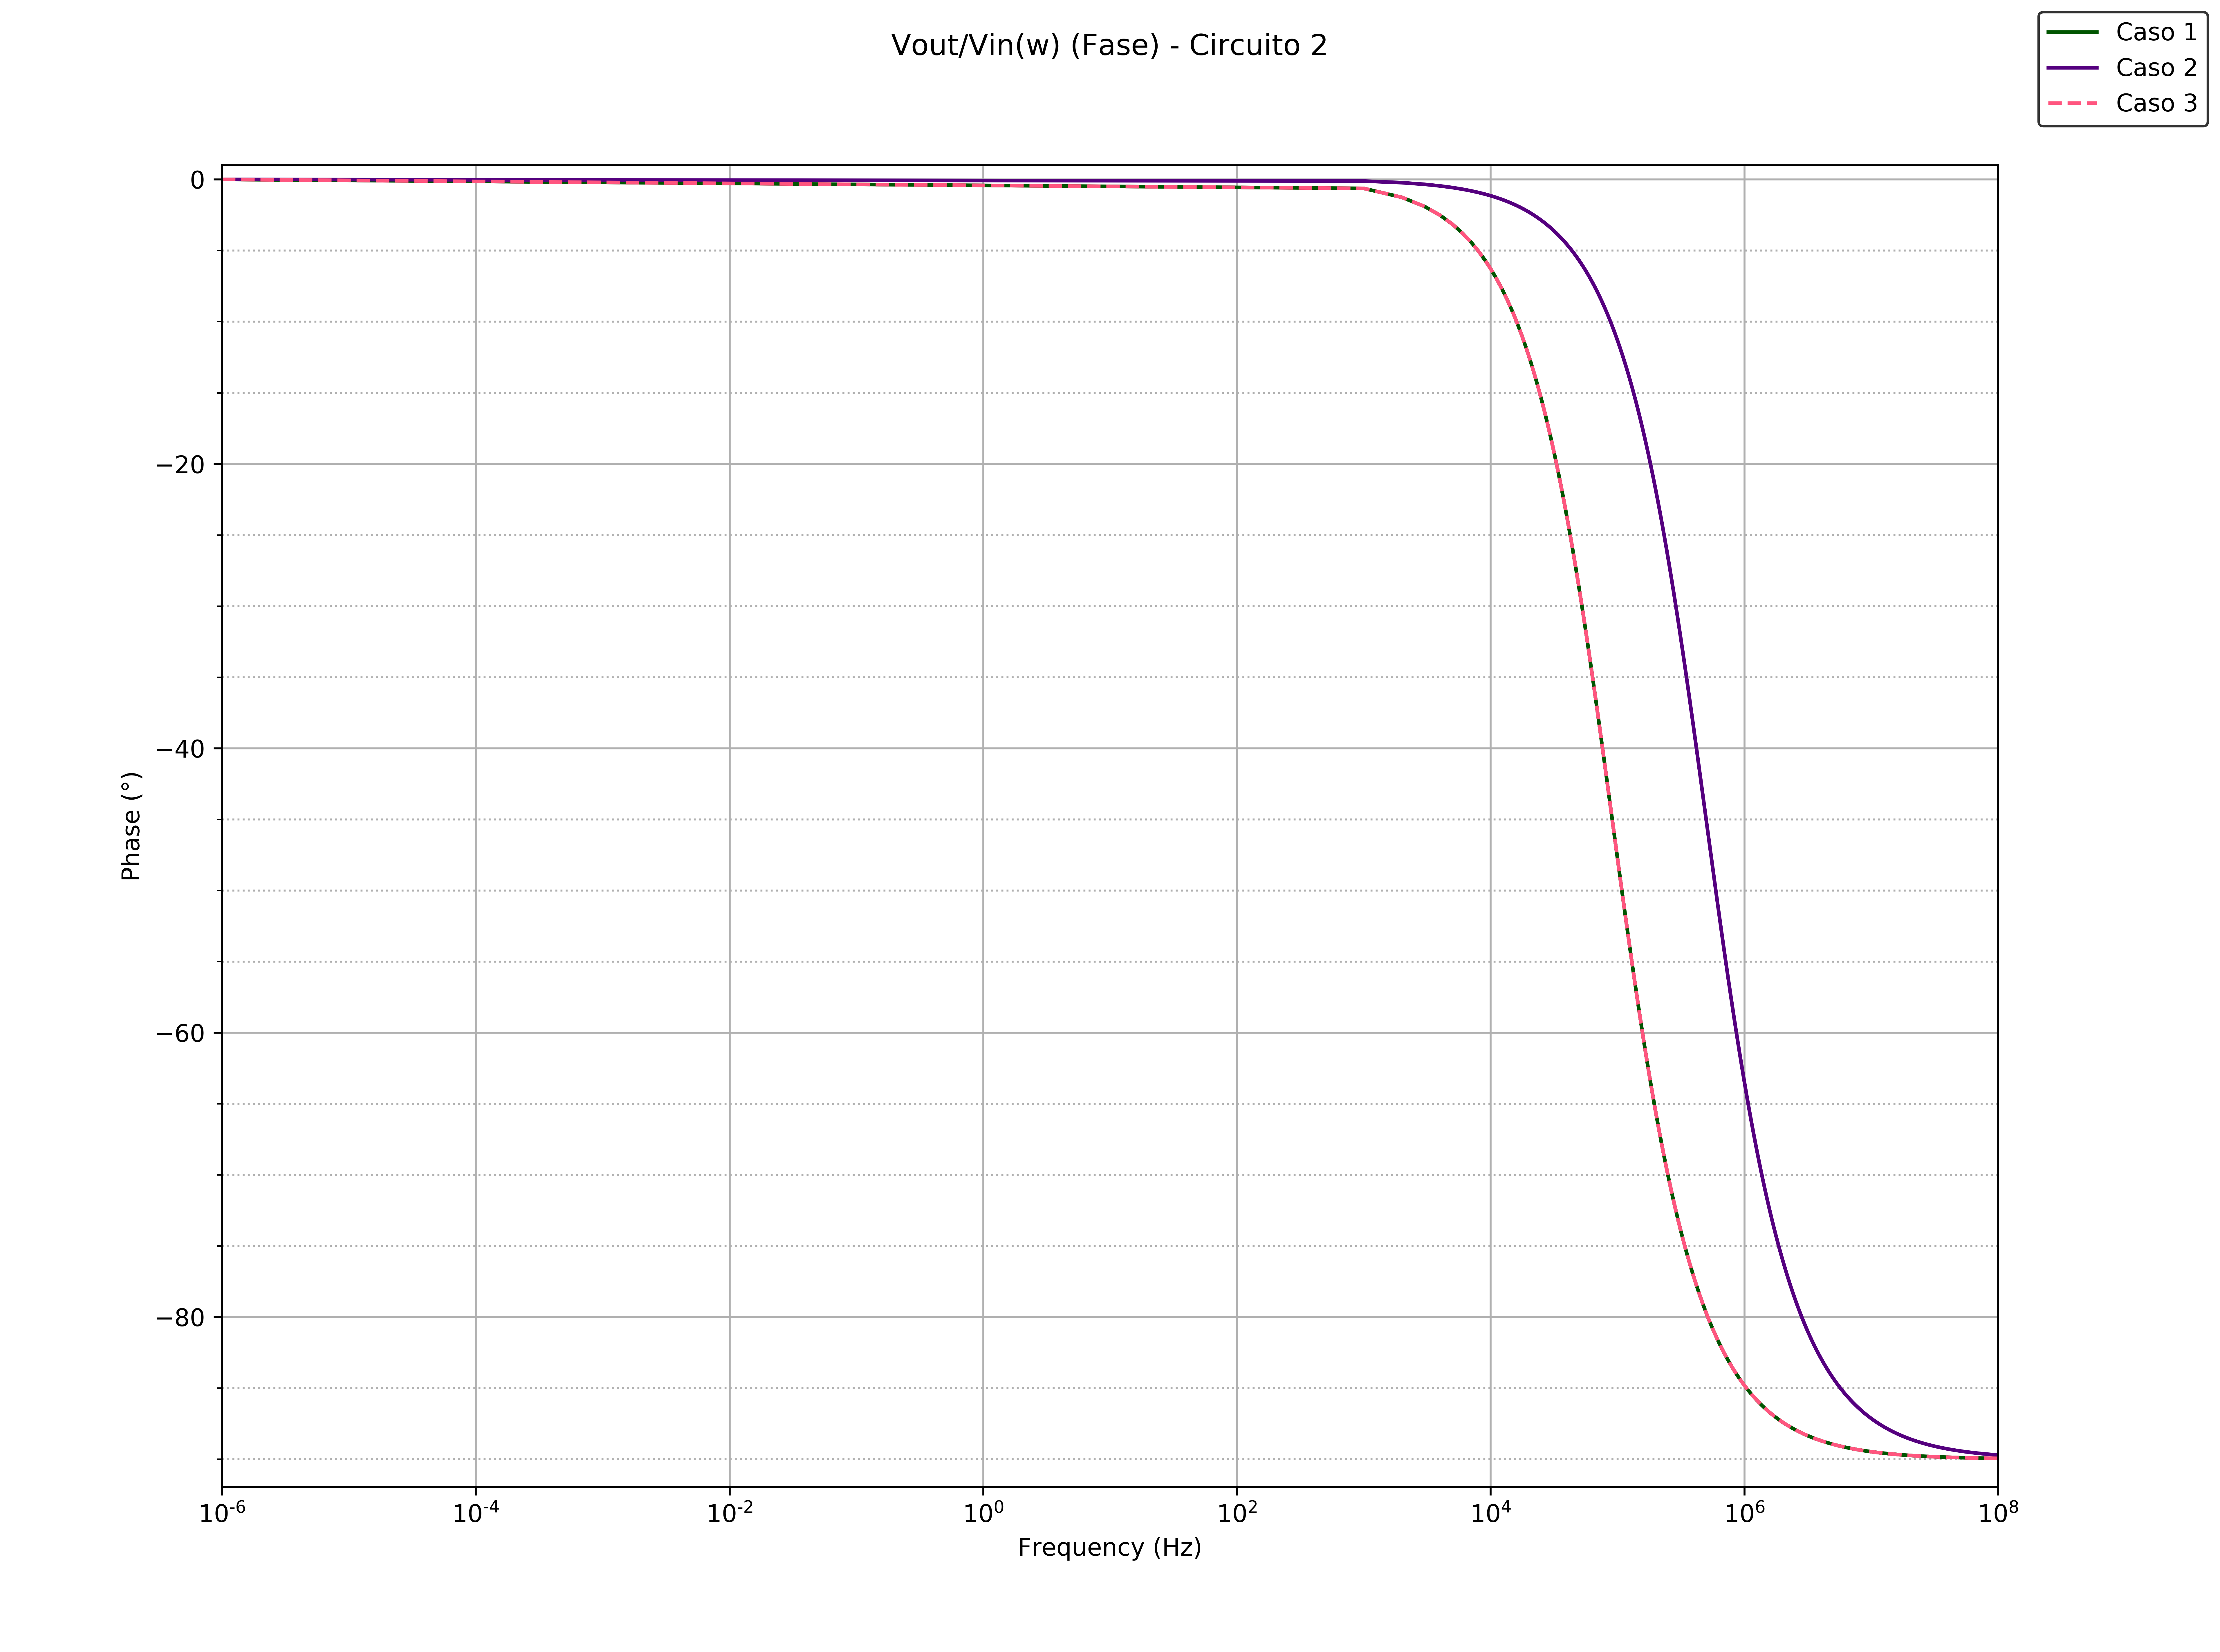
\includegraphics[width=10cm,height=10cm,keepaspectratio]{../EJ1/00GRAFICOS/teoricos/circ2vovifasew.png}
\caption{Configuración no inversora - Comparaci\'on te\'orica de la fase de $V_{out}/V_{in}$ de los tres casos.}
\label{c2voviTeoPh}
\end{figure}

\subsubsection*{Mediciones y resultados obtenidos} %%%%%%

\begin{figure}[H] %!ht
	\centering
	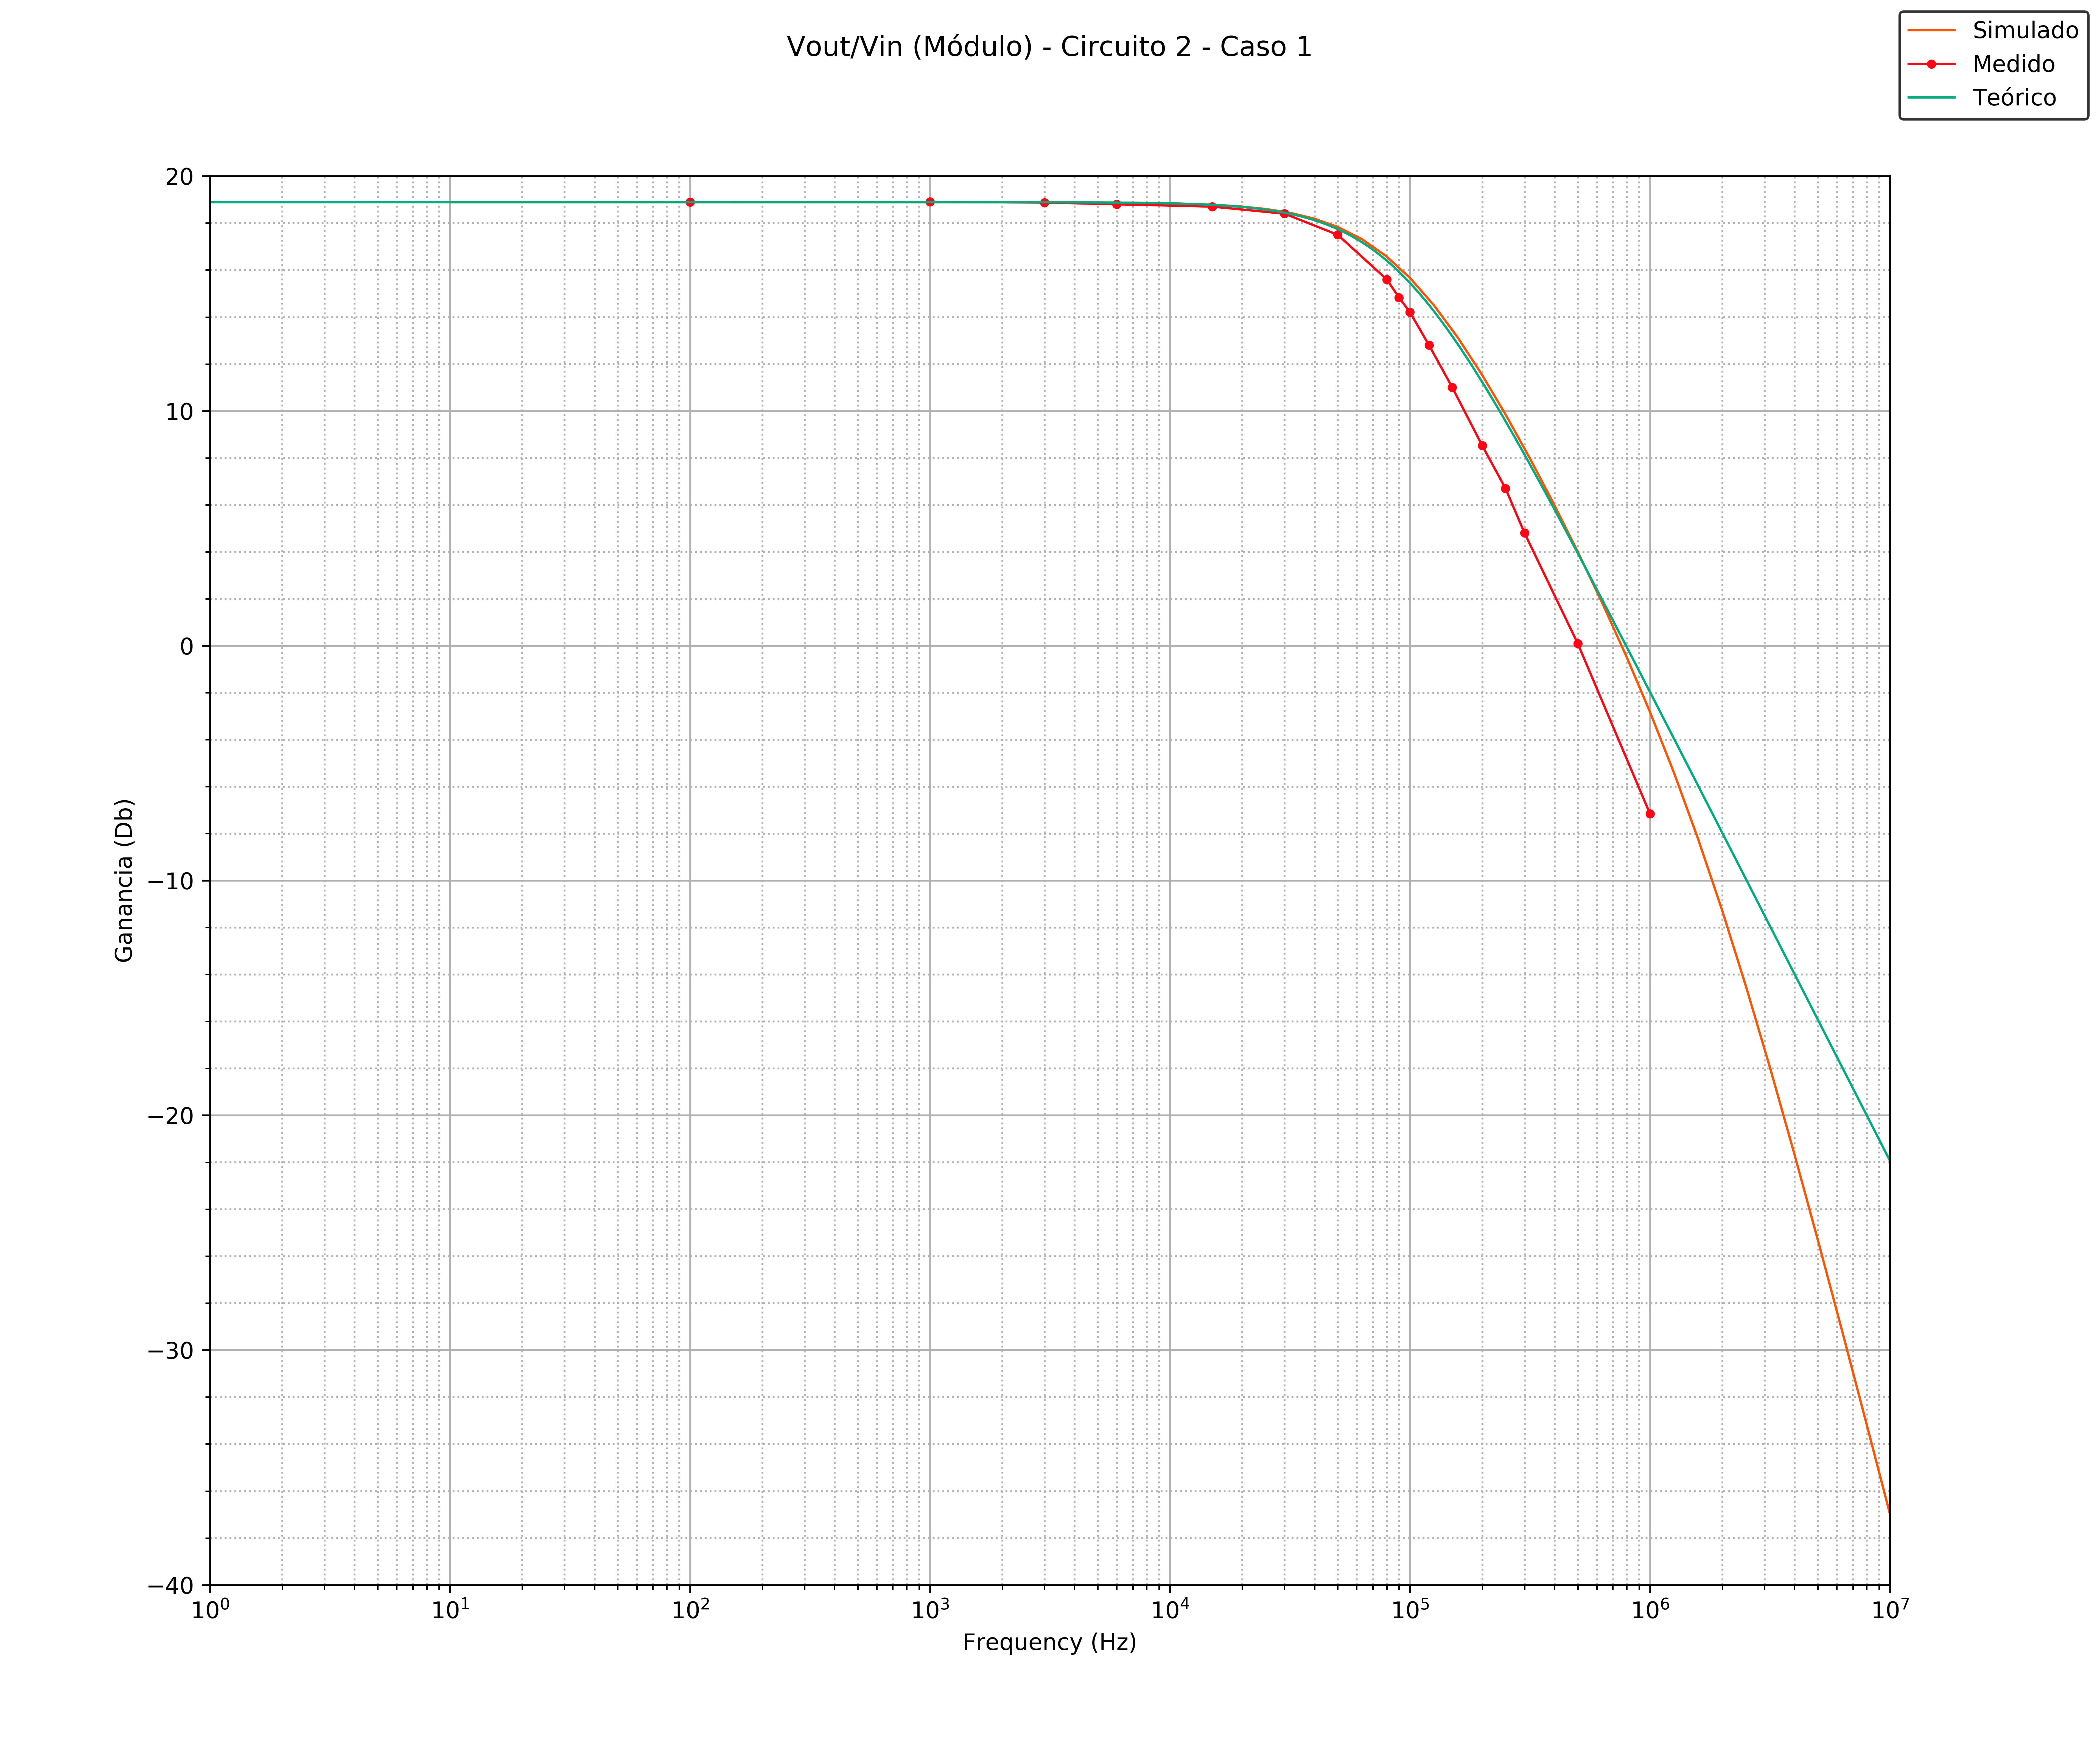
\includegraphics[width=10cm,height=10cm,keepaspectratio]{../EJ1/00GRAFICOS/c2c1/c2c1voviMod.png}
	\caption{Configuración no inversora - Caso 1 -  M\'odulo de $V_{out}/V_{in}$}
	\label{c2c1voviM}
\end{figure}

\begin{figure}[H] %!ht
	\centering
	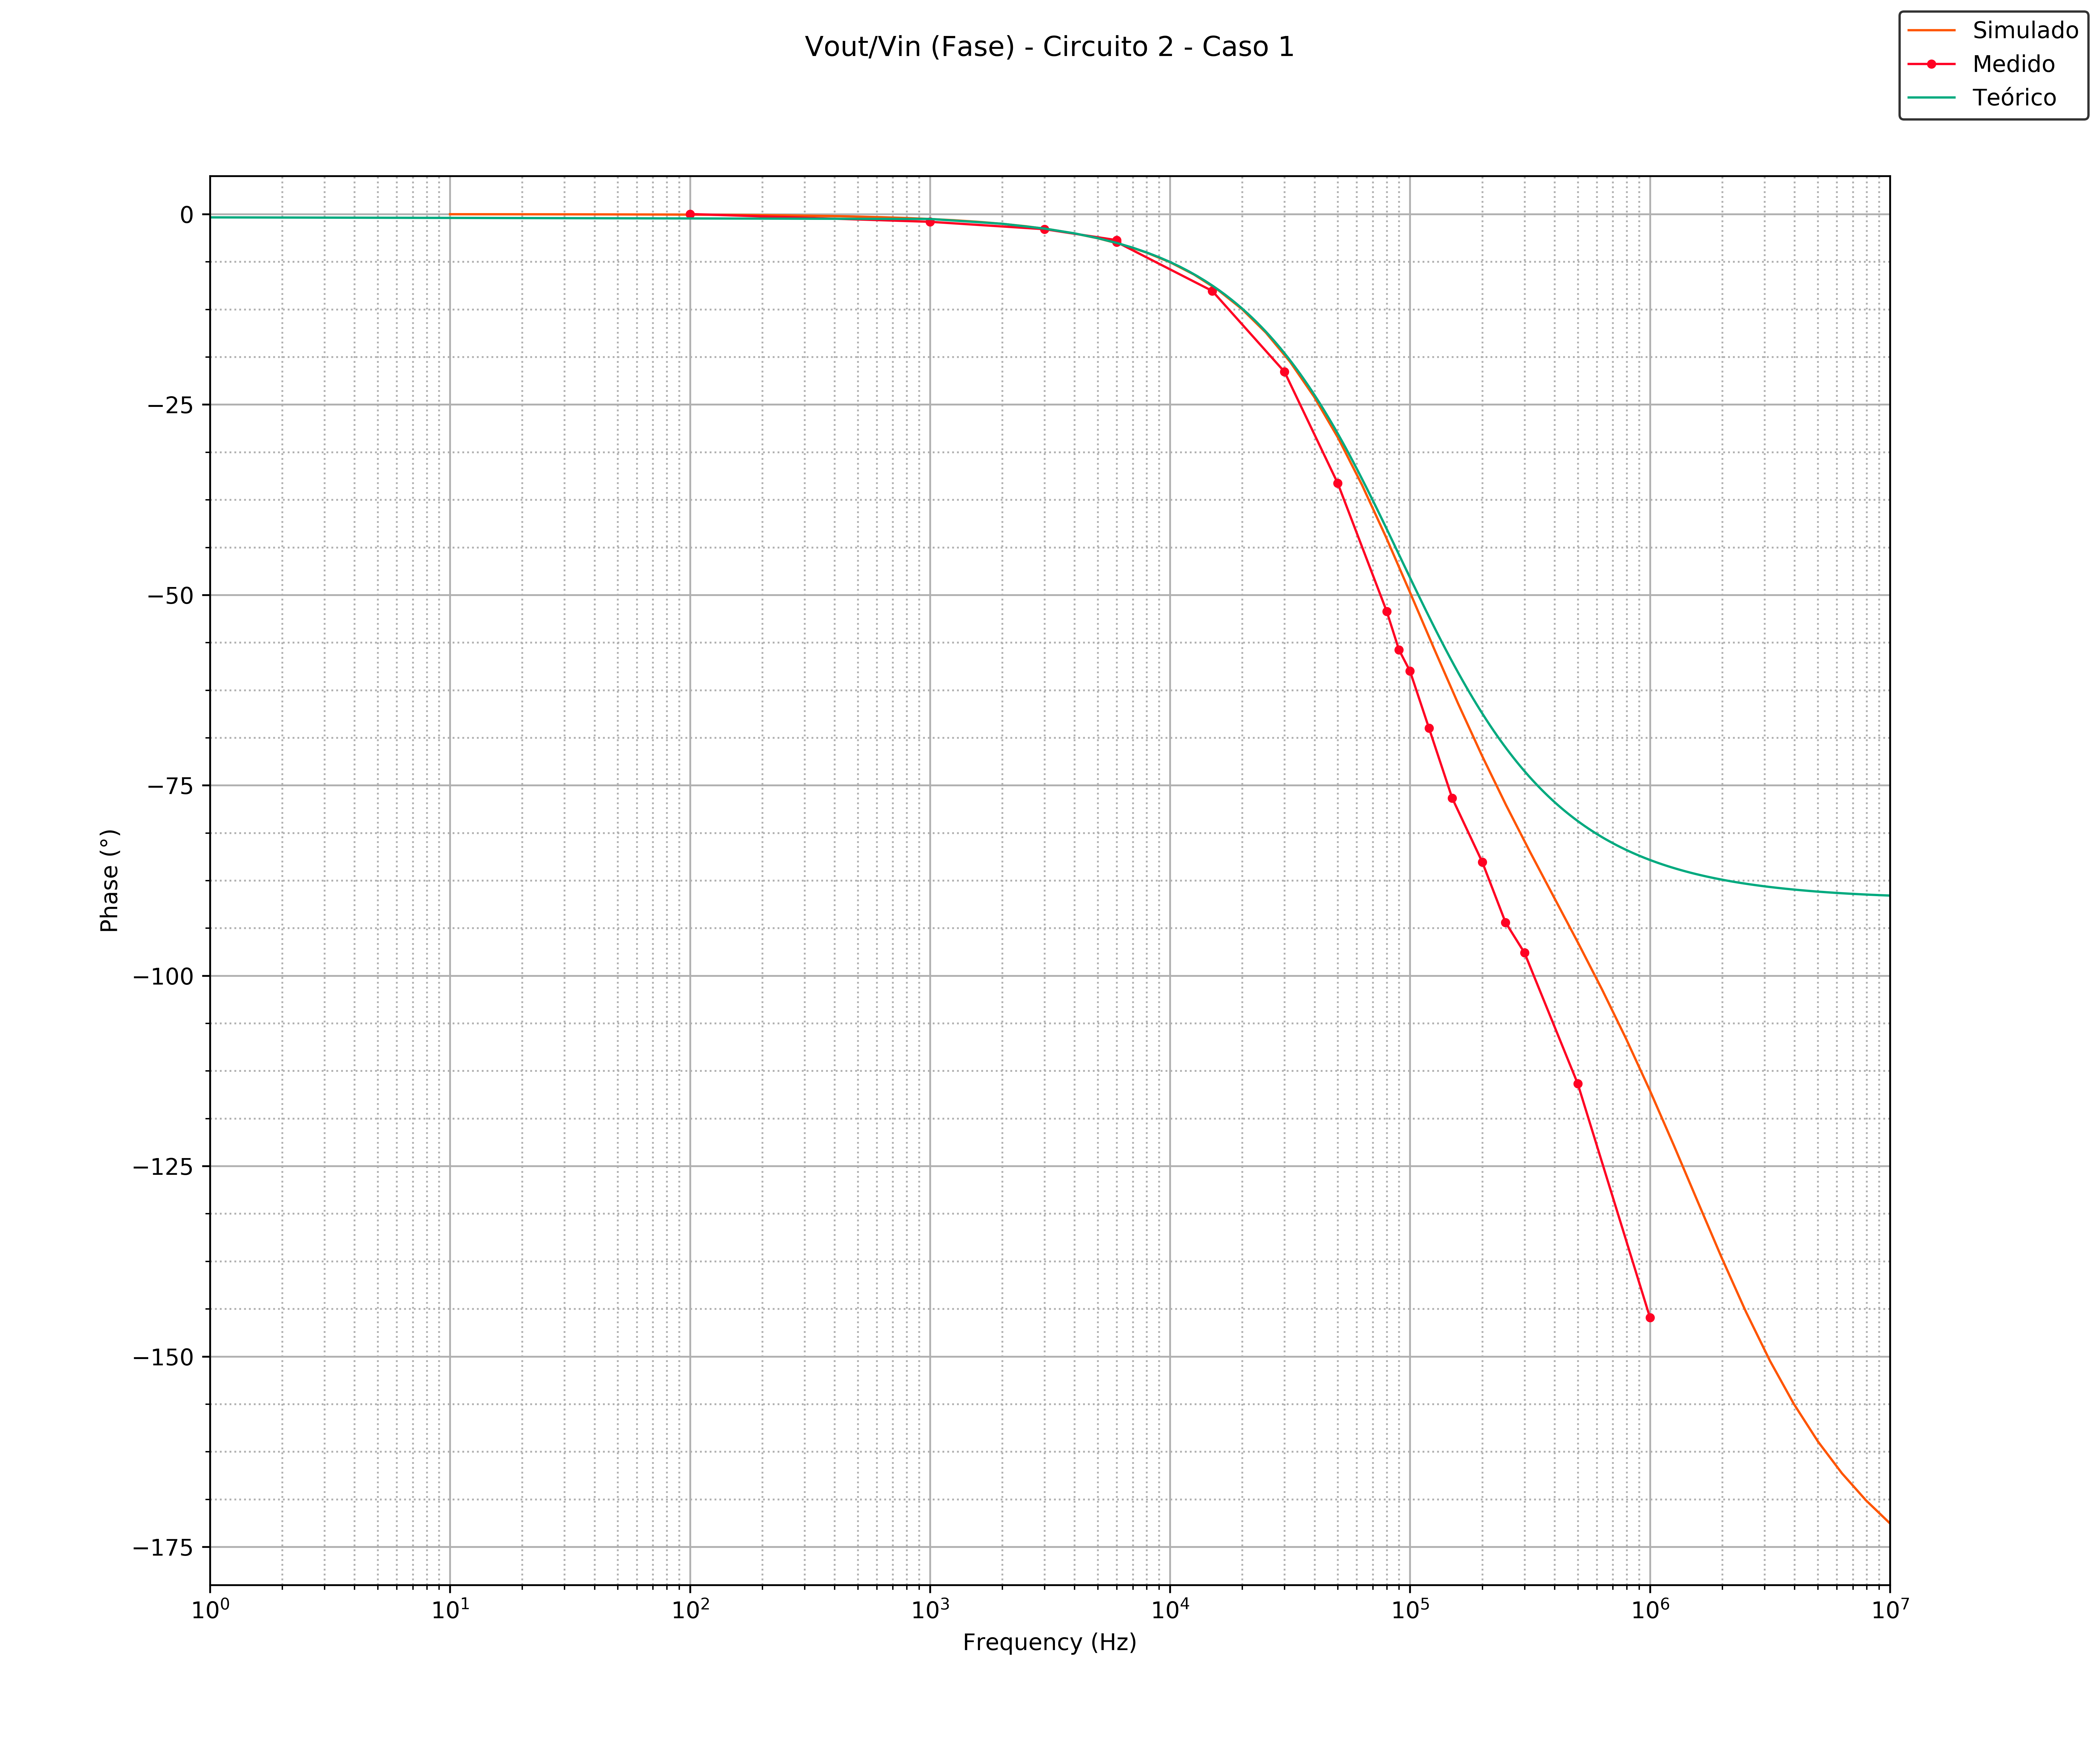
\includegraphics[width=10cm,height=10cm,keepaspectratio]{../EJ1/00GRAFICOS/c2c1/c2c1voviFASE.png}
	\caption{Configuración no inversora - Caso 1 - Fase de $V_{out}/V_{in}$}
	\label{c2c1voviP}
\end{figure}

\begin{figure}[H] %!ht
	\centering
	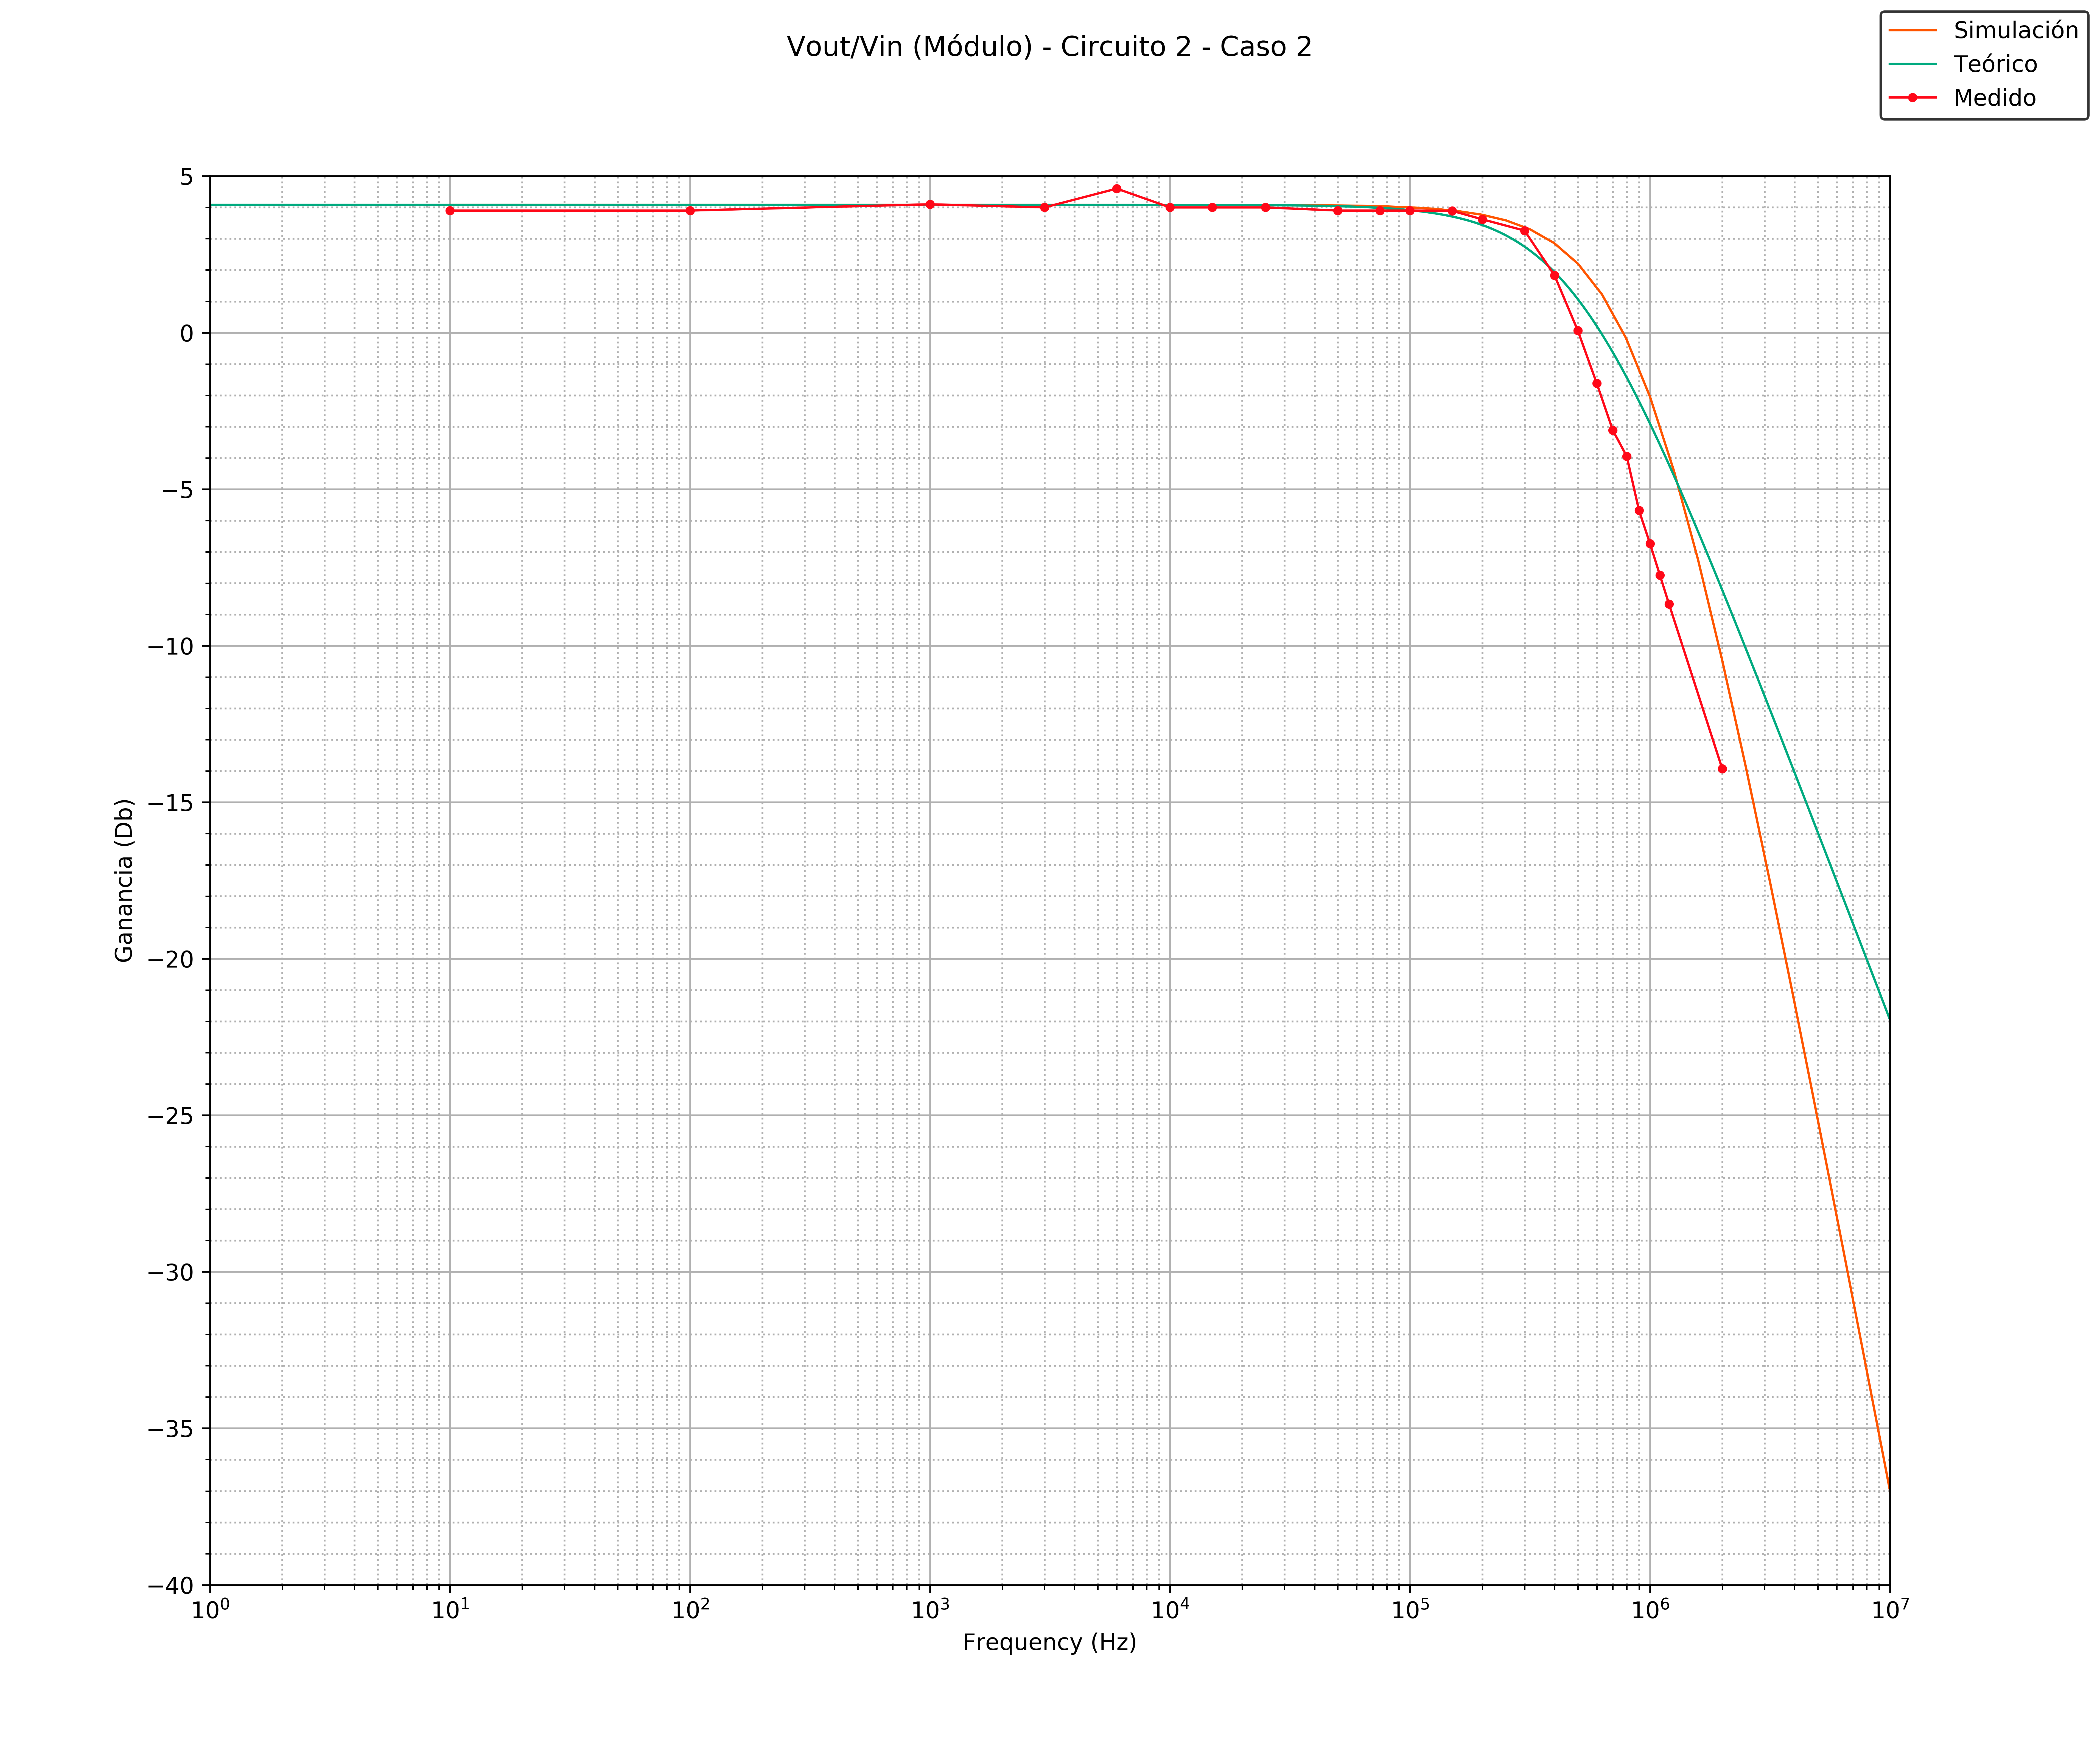
\includegraphics[width=10cm,height=10cm,keepaspectratio]{../EJ1/00GRAFICOS/c2c2/c2c2voviMod.png}
	\caption{Configuración no inversora - Caso 2 - M\'odulo de $V_{out}/V_{in}$}
	\label{c2c2voviM}
\end{figure}

\begin{figure}[H] %!ht
	\centering
	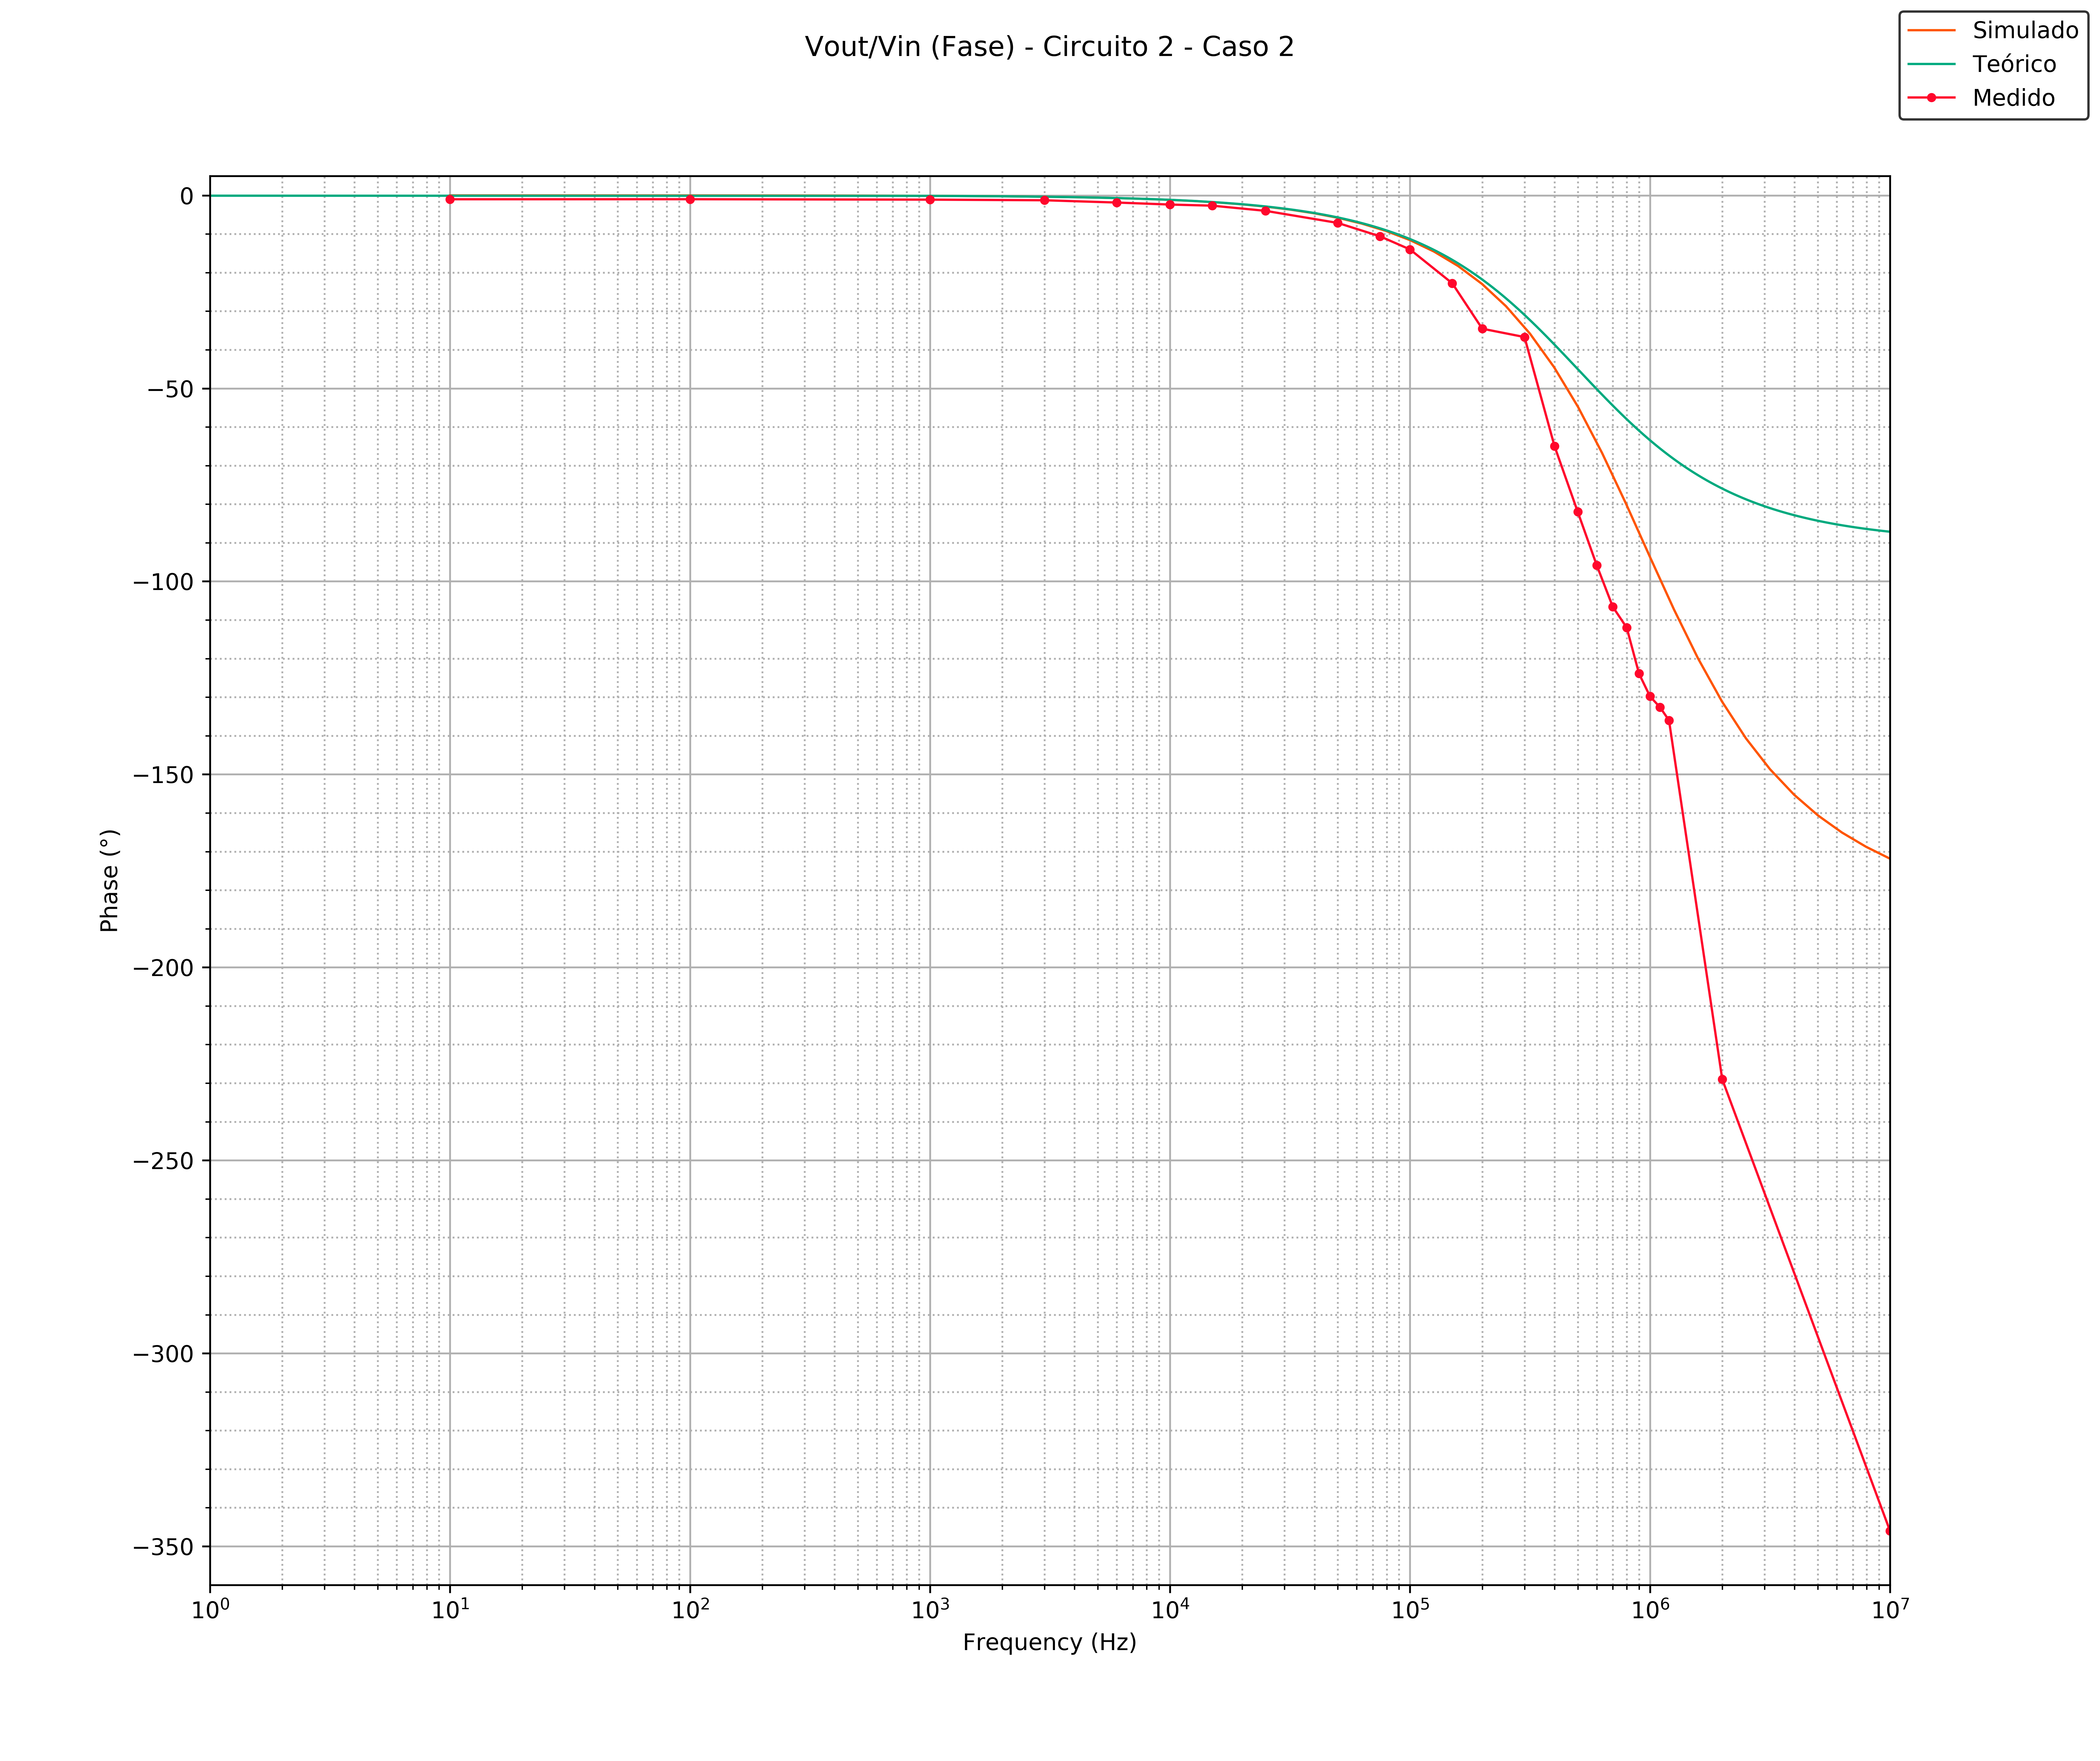
\includegraphics[width=10cm,height=10cm,keepaspectratio]{../EJ1/00GRAFICOS/c2c2/c2c2voviFASE.png}
	\caption{Configuración no inversora - Caso 2 - Fase de $V_{out}/V_{in}$}
	\label{c2c2voviP}
\end{figure}

%\begin{figure}[H] %!ht
%	\centering
%	\includegraphics[width=10cm,height=10cm,keepaspectratio]{../EJ1/00GRAFICOS/c2c3/c2c3voviMod.png}
%	\caption{Configuración no inversora - Caso 3 - M\'odulo de $V_{out}/V_{in}$}	
%	\label{c2c3voviM}
%\end{figure}

\begin{figure}[H] %!ht
	\centering
	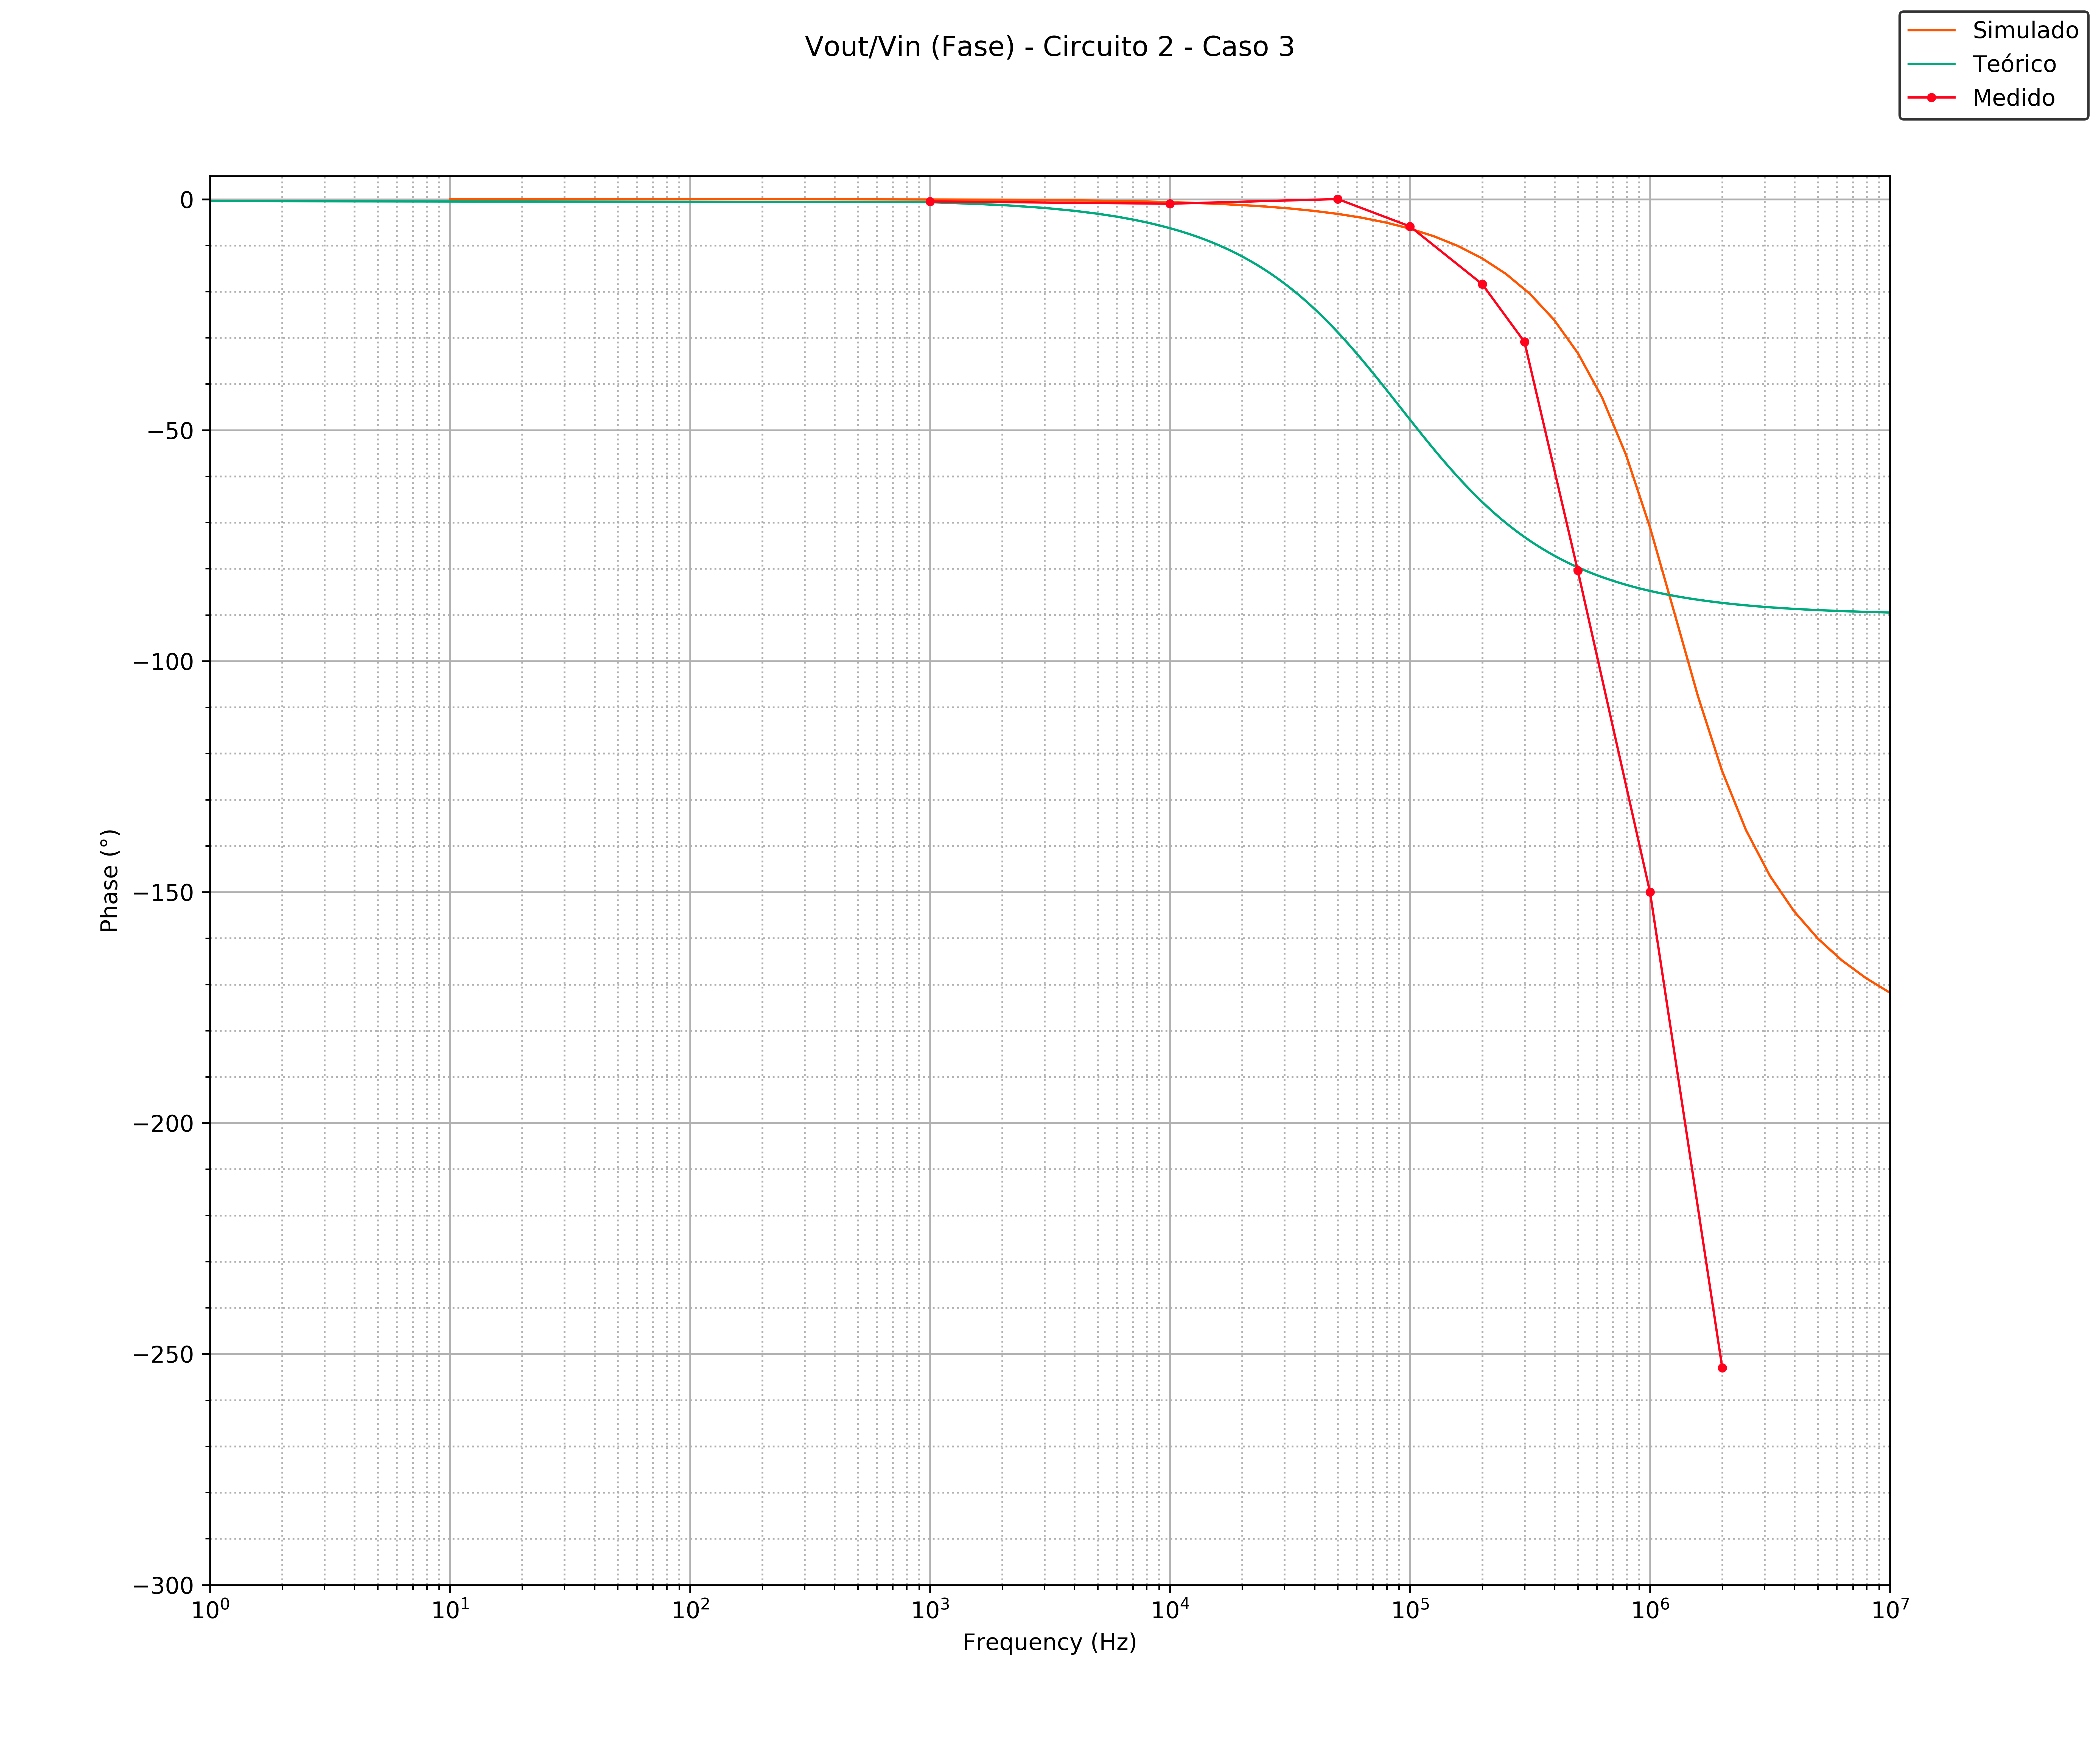
\includegraphics[width=10cm,height=10cm,keepaspectratio]{../EJ1/00GRAFICOS/c2c3/c2c3voviFASE.png}
	\caption{Configuración no inversora - Caso 3 - Fase de $V_{out}/V_{in}$}
	\label{c2c3voviP}
\end{figure}


\subsubsection{Impedancia de entrada del circuito}%%%%%%

\subsubsection*{An\'alisis te\'orico} %%%%%%
%GRAFICAR Y PONER FORMULAS!!!!!!!!!!!!!!!

\subsubsection*{Mediciones y resultados obtenidos} %%%%%%
\begin{figure}[H] %!ht
	\centering
	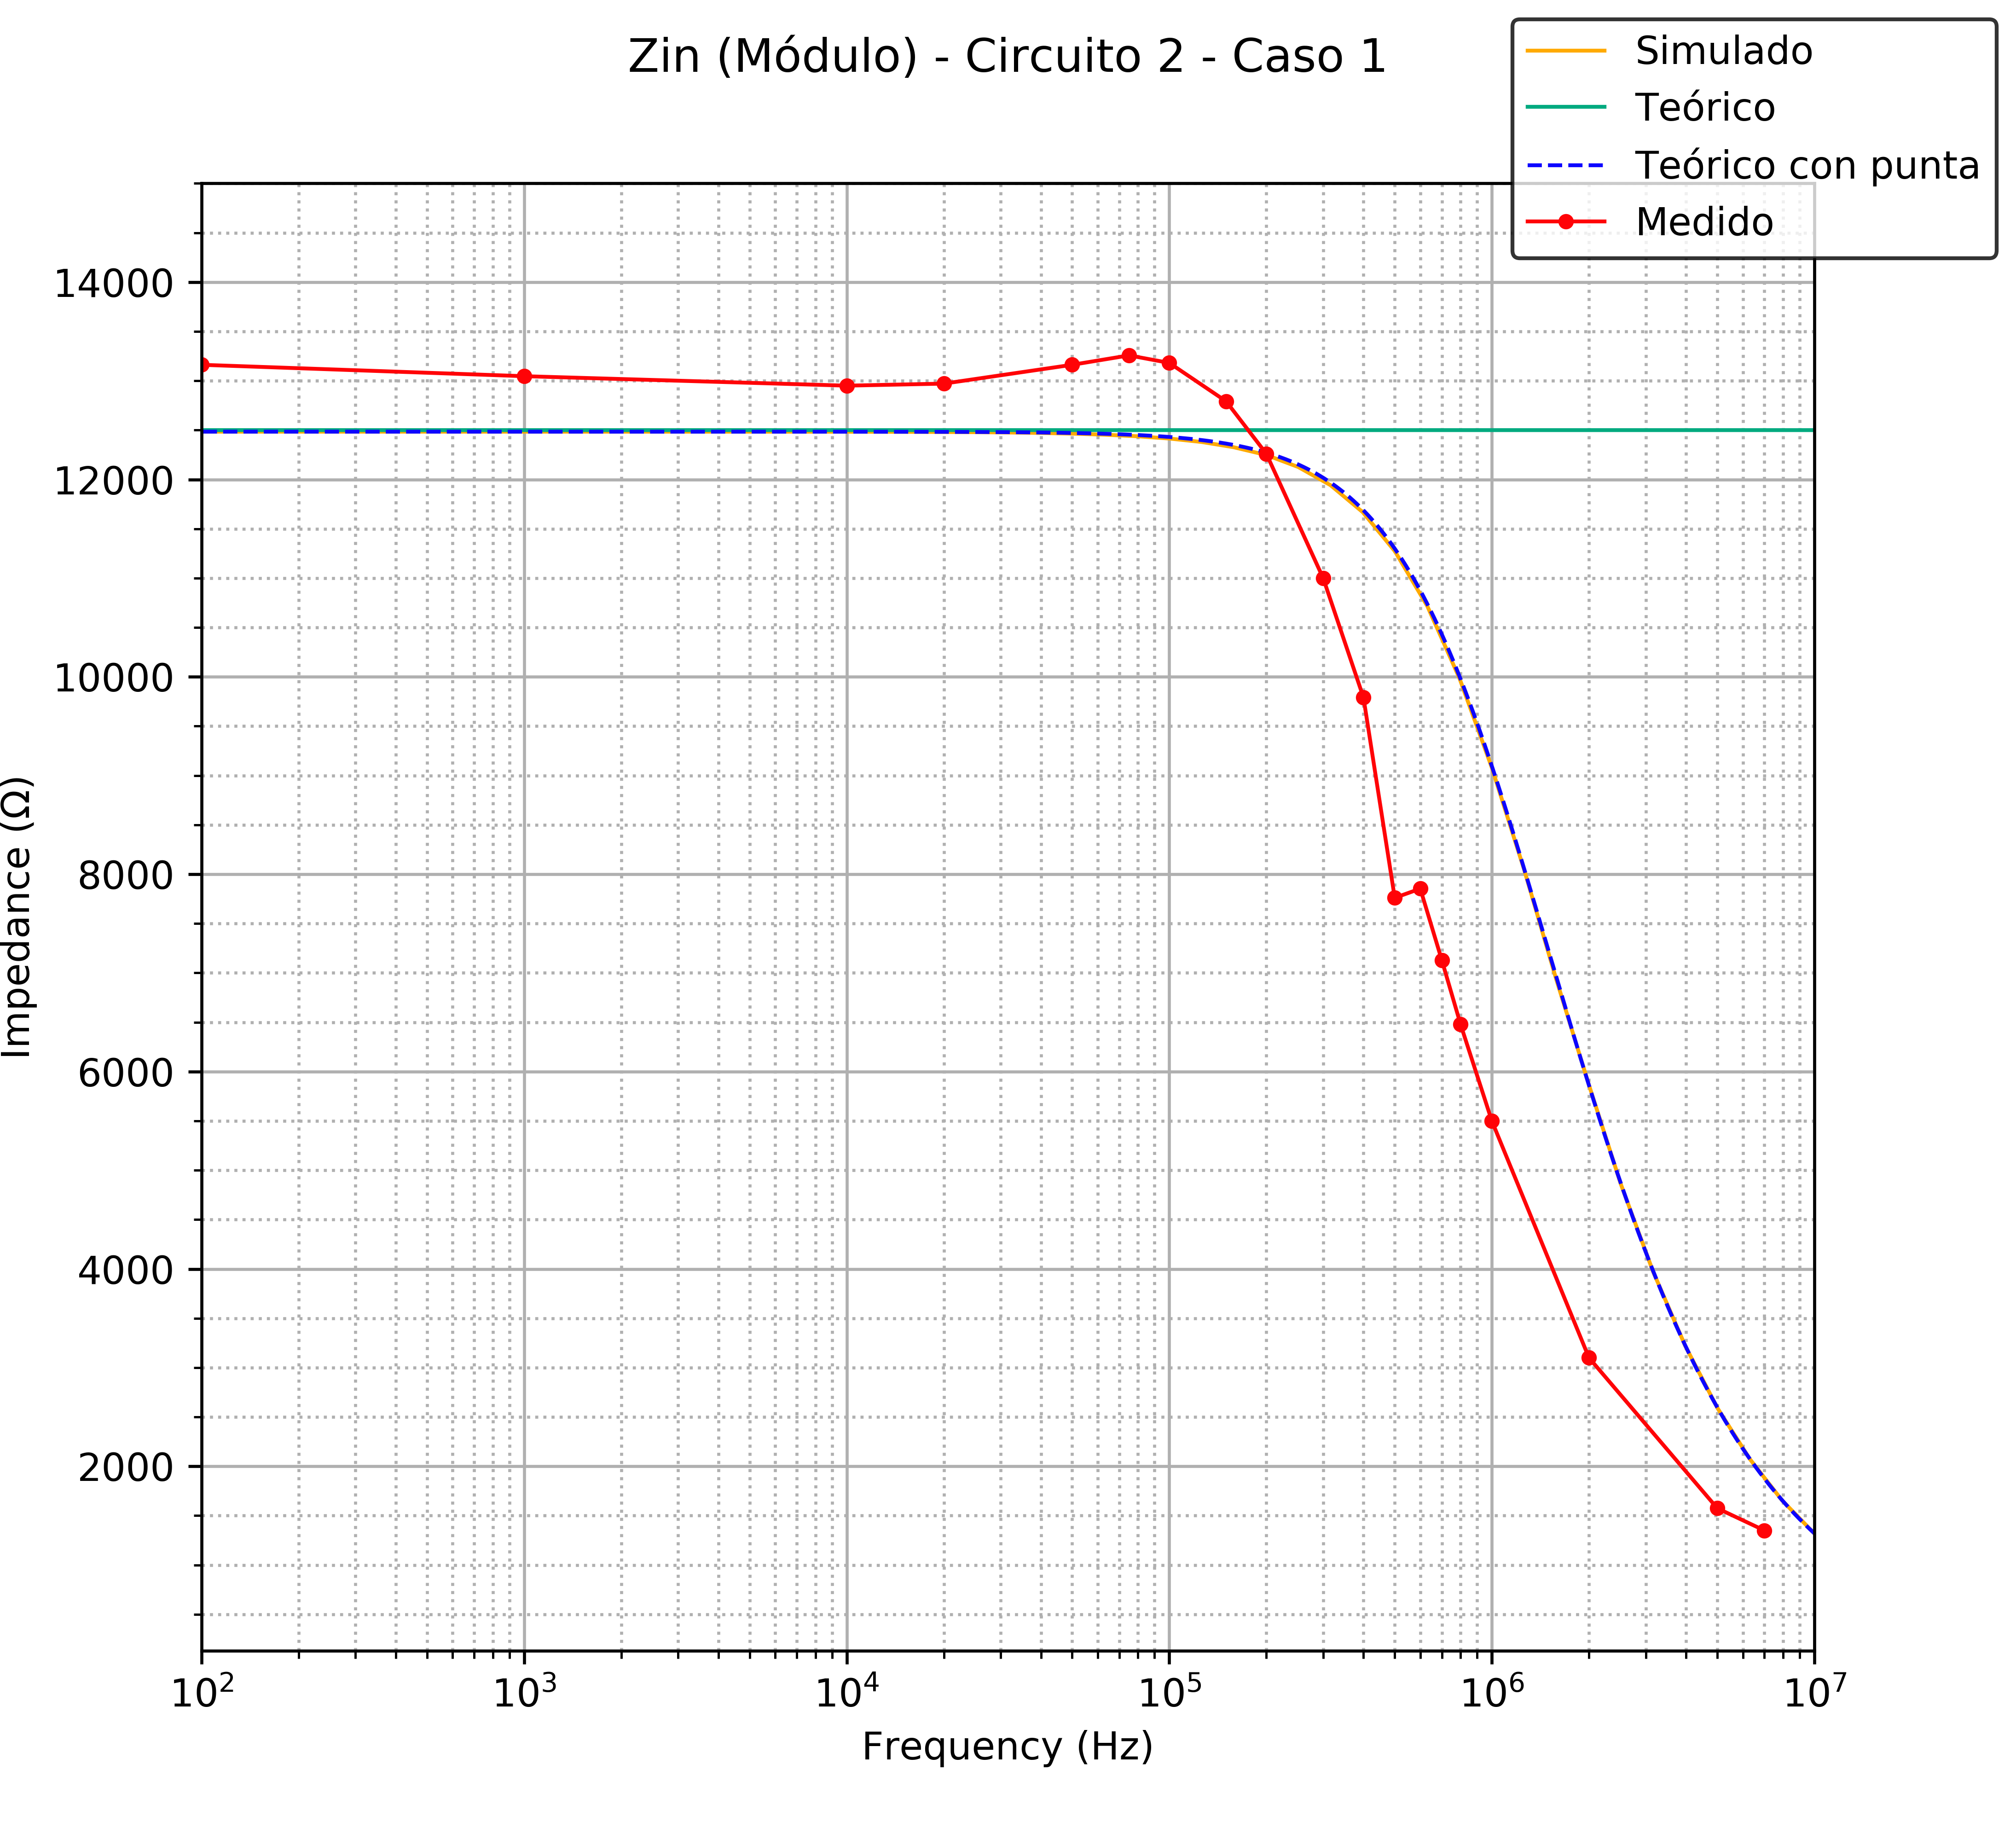
\includegraphics[width=10cm,height=10cm,keepaspectratio]{../EJ1/00GRAFICOS/c2c1/c2c1ZINpunta.png}
	\caption{Configuración no inversora - Caso 1 - M\'odulo de $Z_{in}$}
	\label{c2c1zinM}
\end{figure}

\begin{figure}[H] %!ht
	\centering
	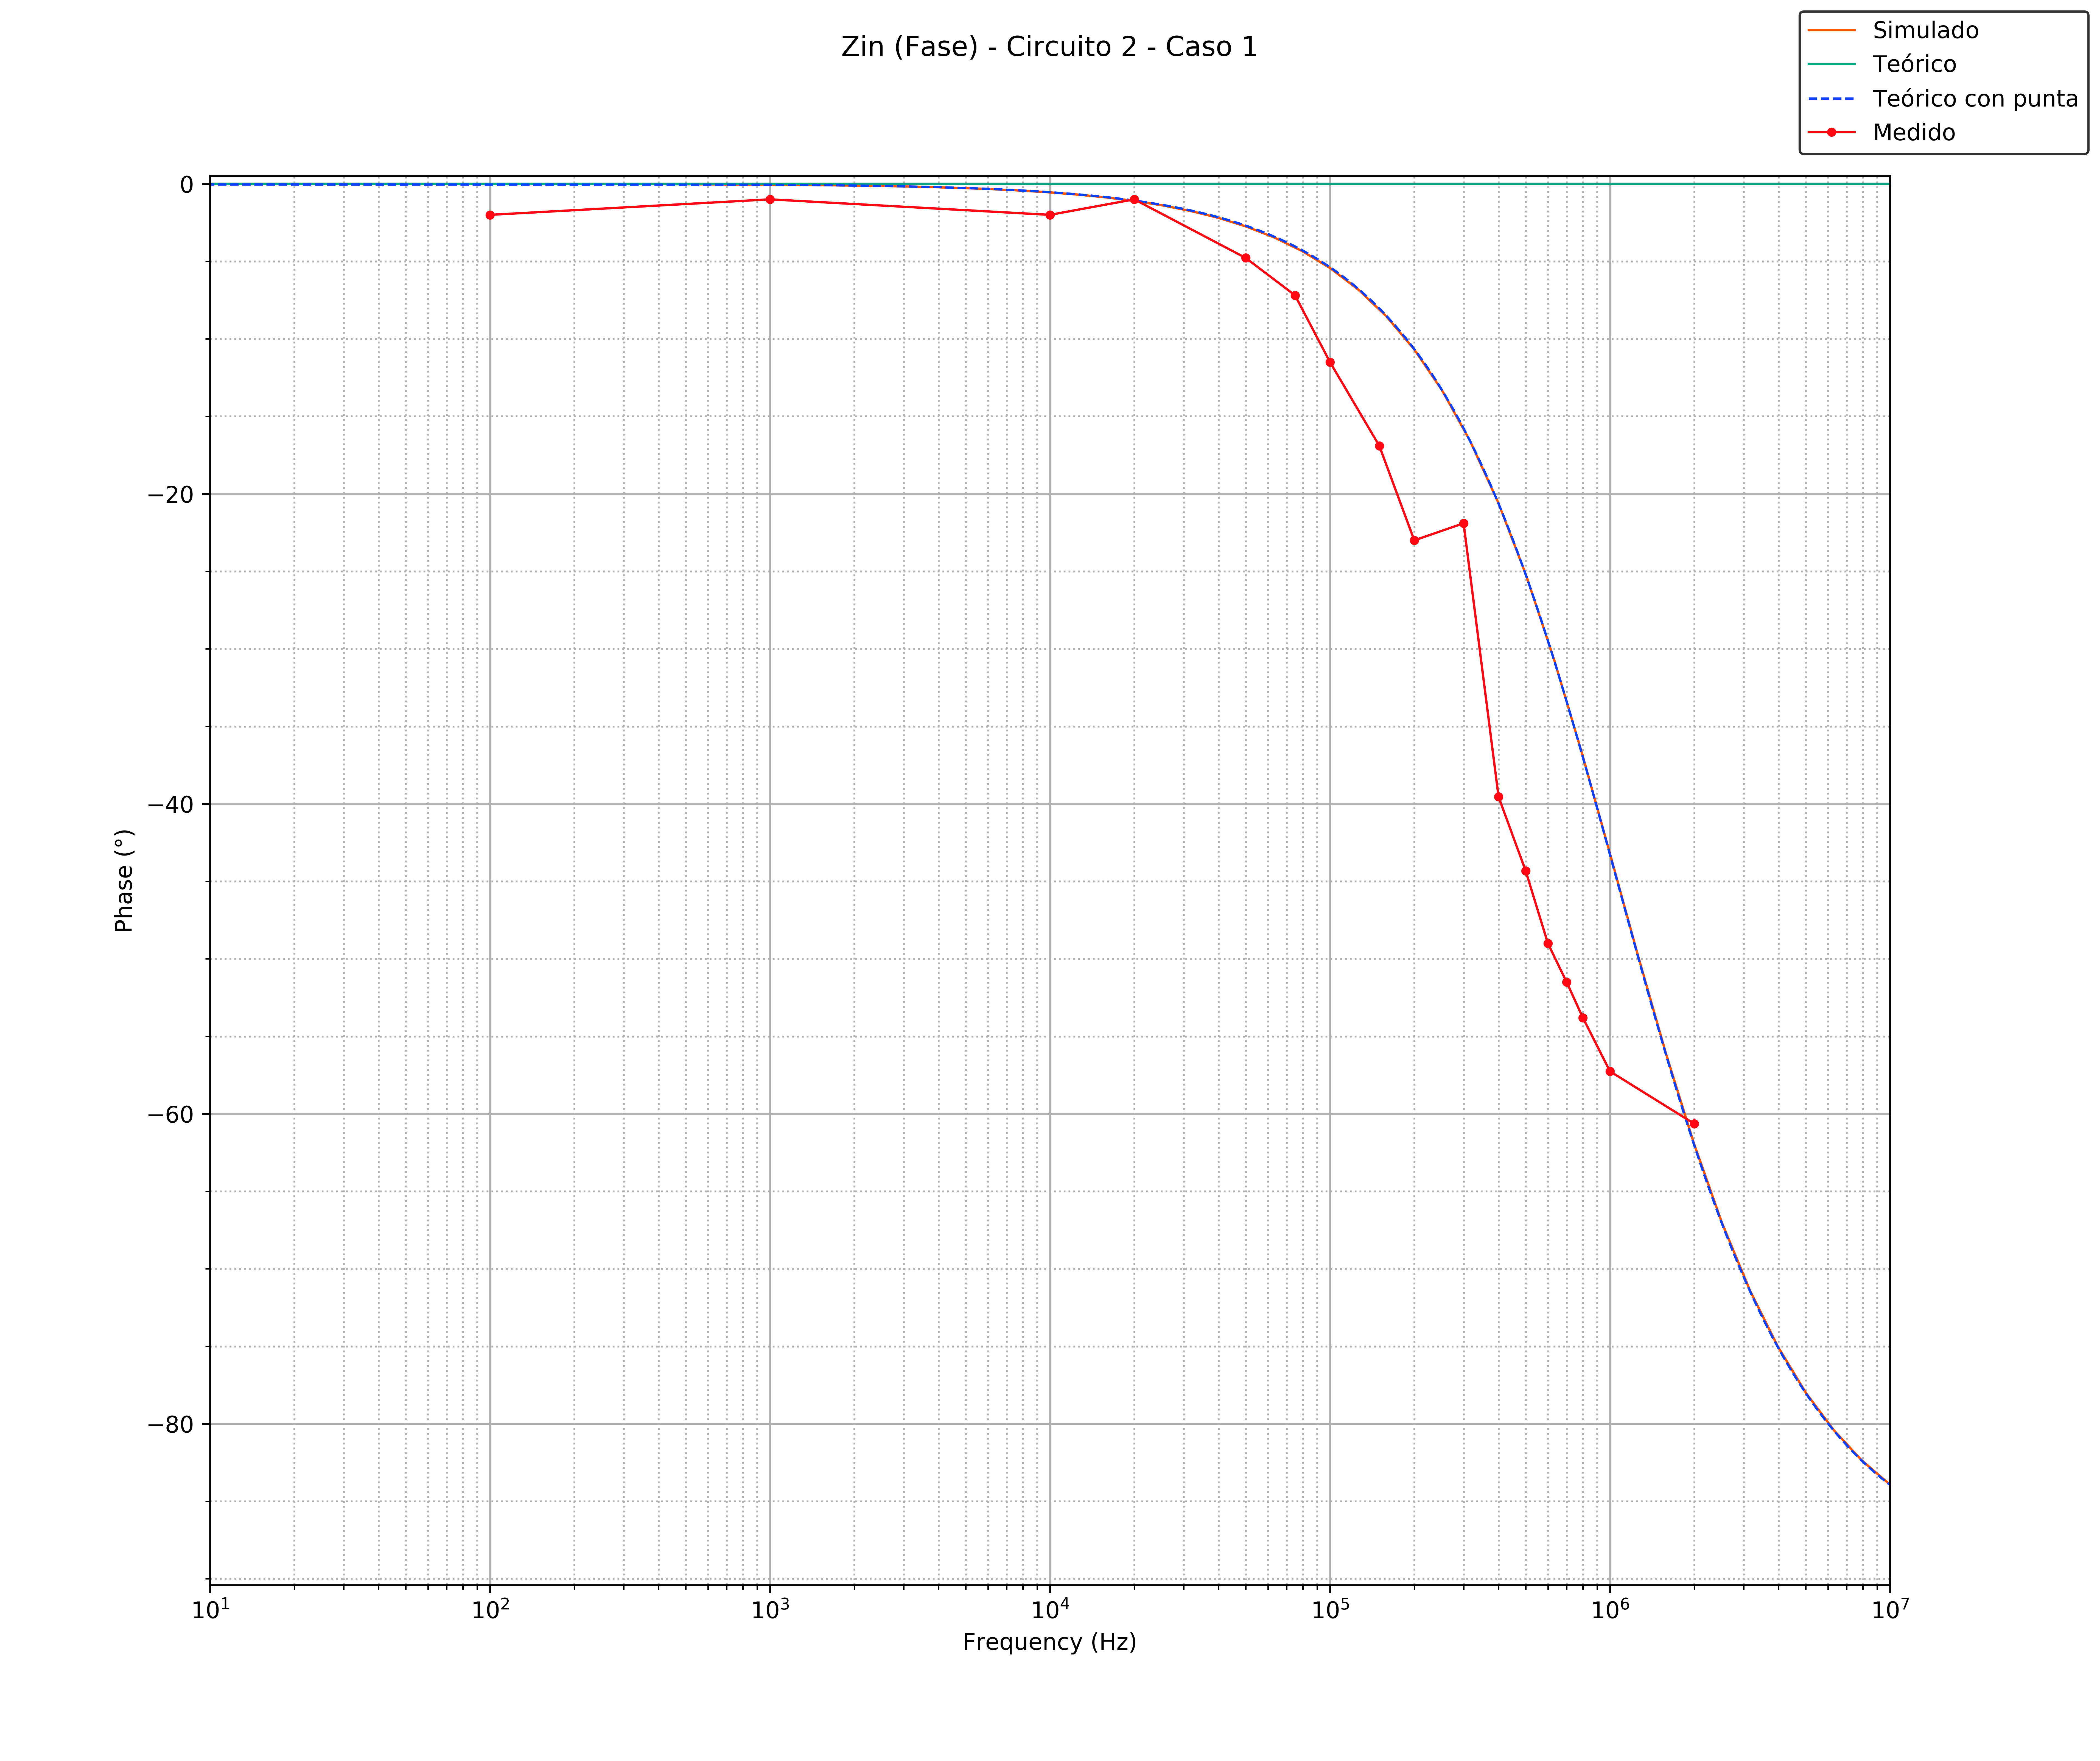
\includegraphics[width=10cm,height=10cm,keepaspectratio]{../EJ1/00GRAFICOS/c2c1/c2c1zinFASE.png}
	\caption{Configuración no inversora - Caso 1 - Fase de $Z_{in}$}
	\label{c2c1zinP}
\end{figure}

\begin{figure}[H] %!ht
	\centering
	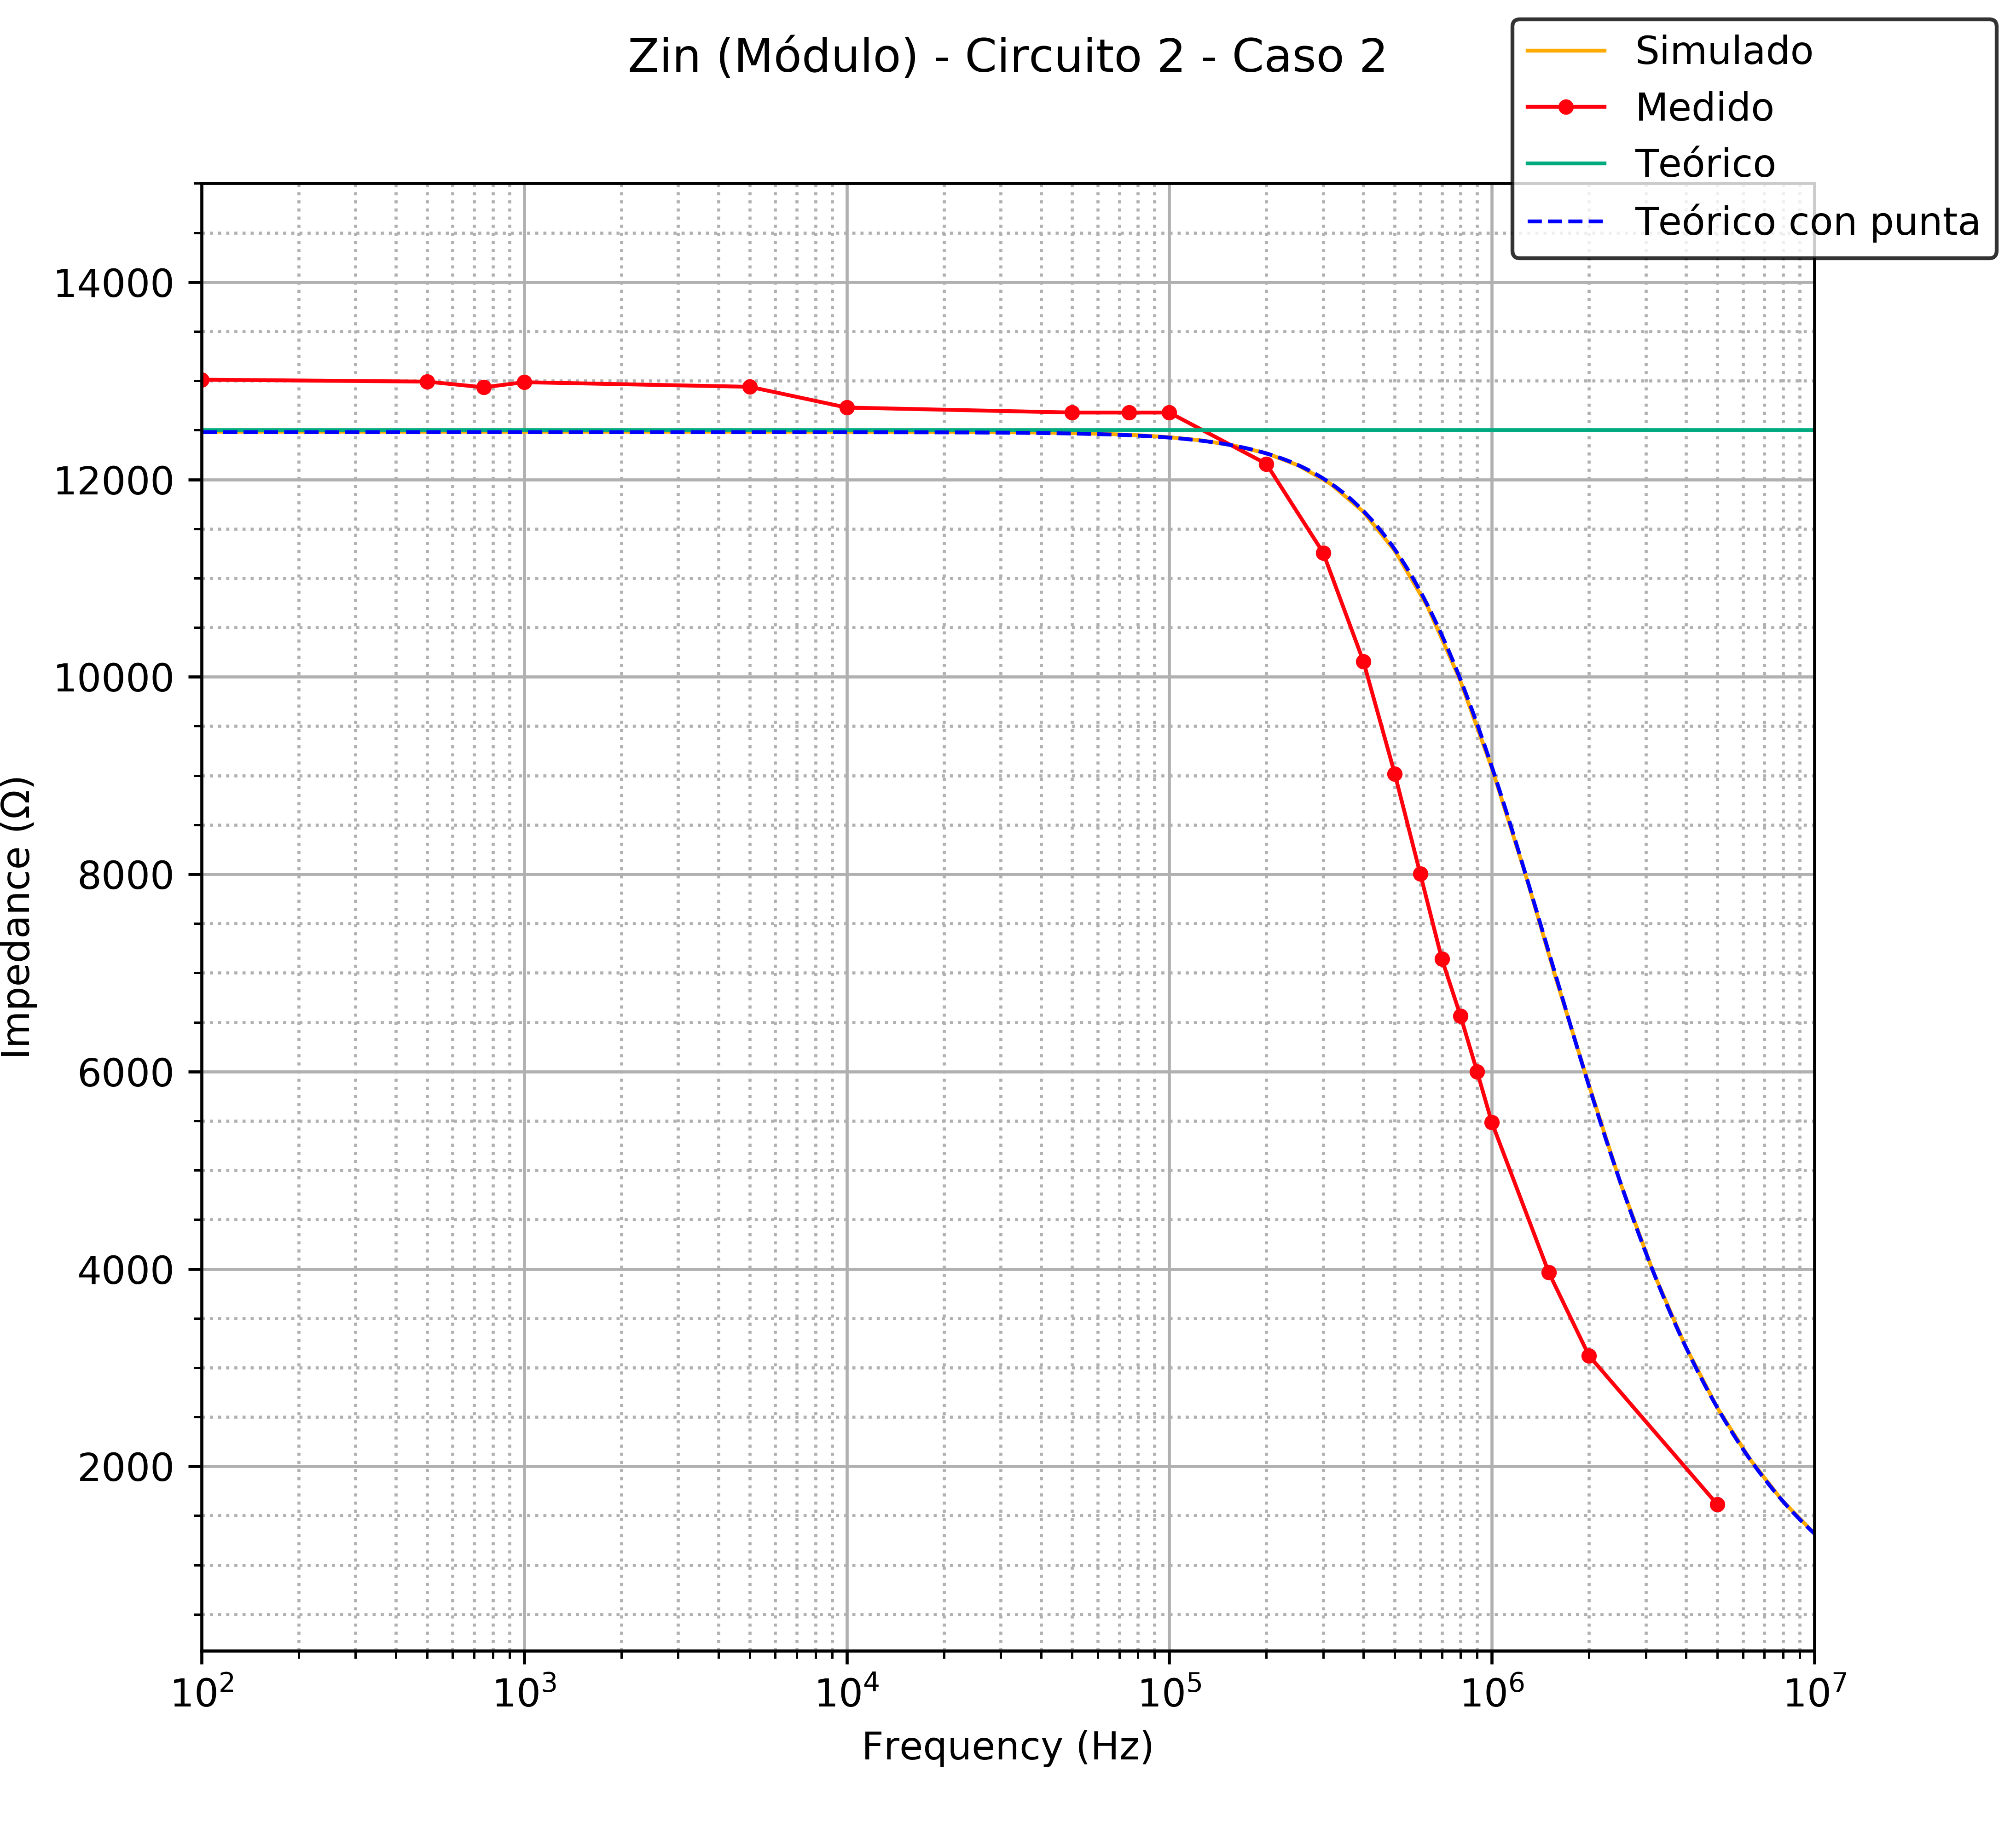
\includegraphics[width=10cm,height=10cm,keepaspectratio]{../EJ1/00GRAFICOS/c2c2/c2c2ZINpunta.png}
	\caption{Configuración no inversora - Caso 2 - M\'odulo de $Z_{in}$}
	\label{c2c2zinM}
\end{figure}

\begin{figure}[H] %!ht
	\centering
	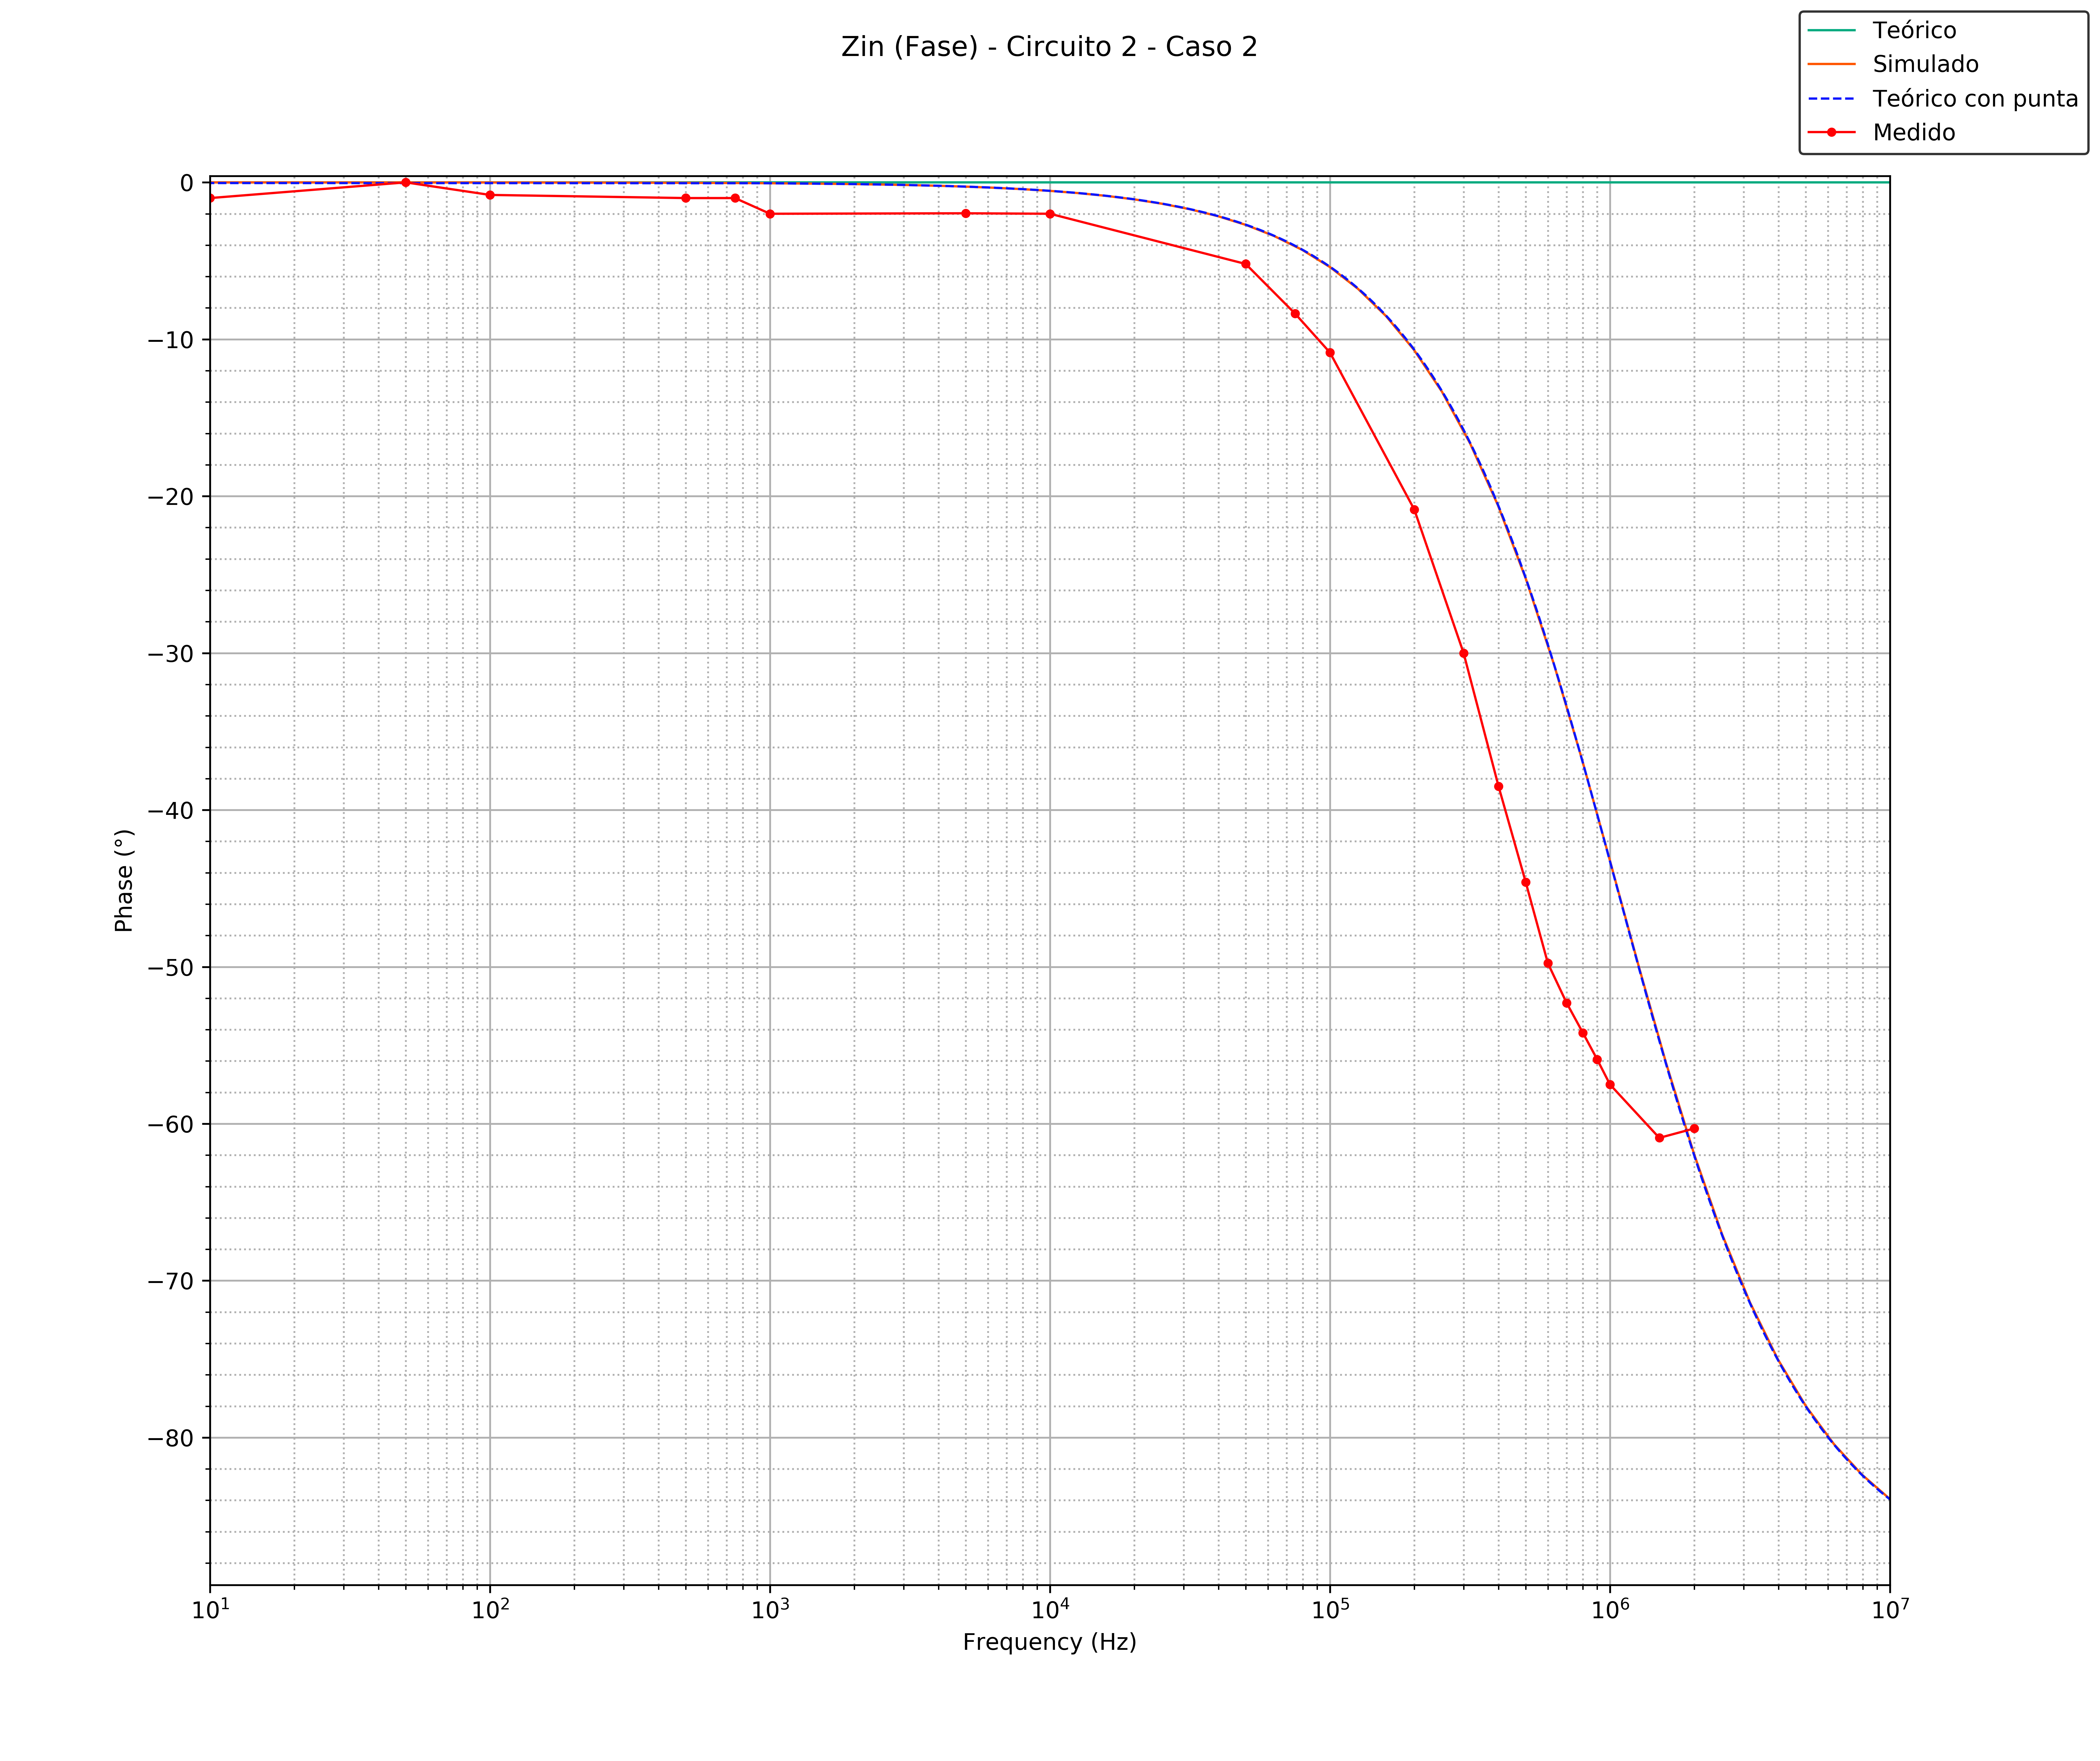
\includegraphics[width=10cm,height=10cm,keepaspectratio]{../EJ1/00GRAFICOS/c2c2/c2c2zinFASE.png}
	\caption{Configuración no inversora - Caso 2 - Fase de $Z_{in}$}
	\label{c2c2zinP}
\end{figure}

%\begin{figure}[H] %!ht
%	\centering
%	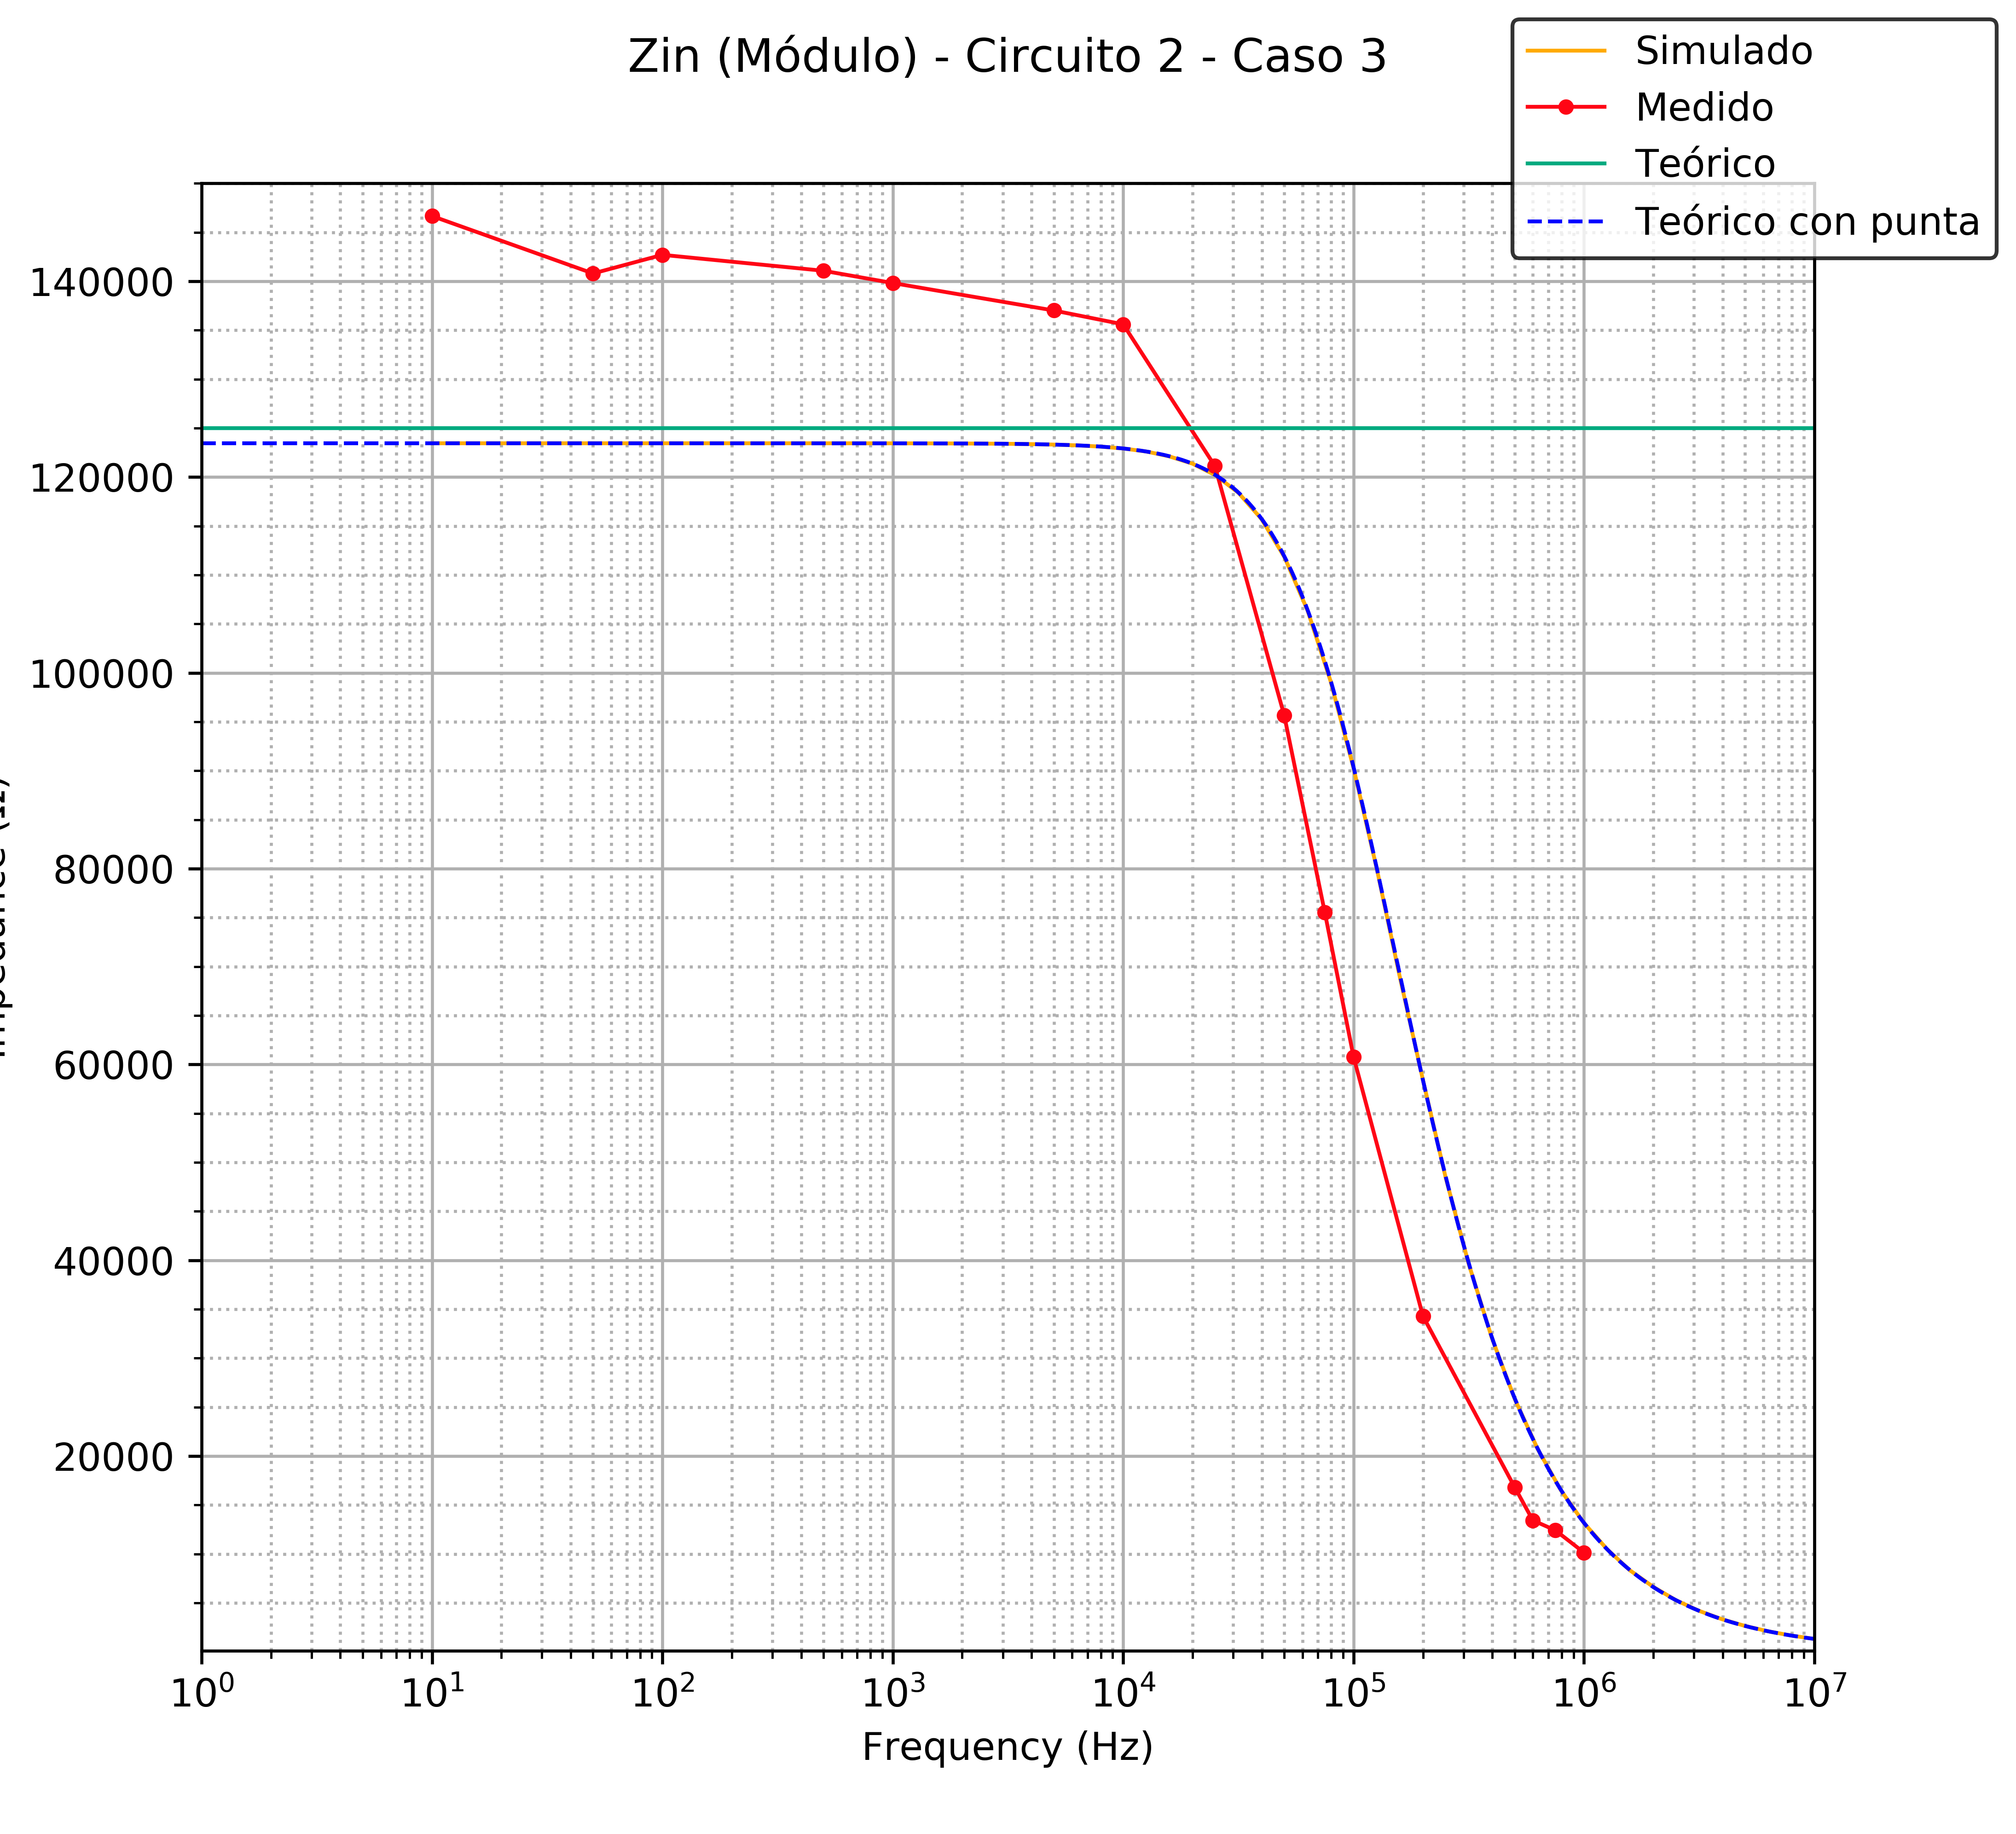
\includegraphics[width=10cm,height=10cm,keepaspectratio]{../EJ1/00GRAFICOS/c2c3/c2c3ZINpunta.png}
%	\caption{Configuración no inversora - Caso 3 - M\'odulo de $Z_{in}$}
%	\label{c2c3zinM}
%\end{figure}

\begin{figure}[H] %!ht
	\centering
	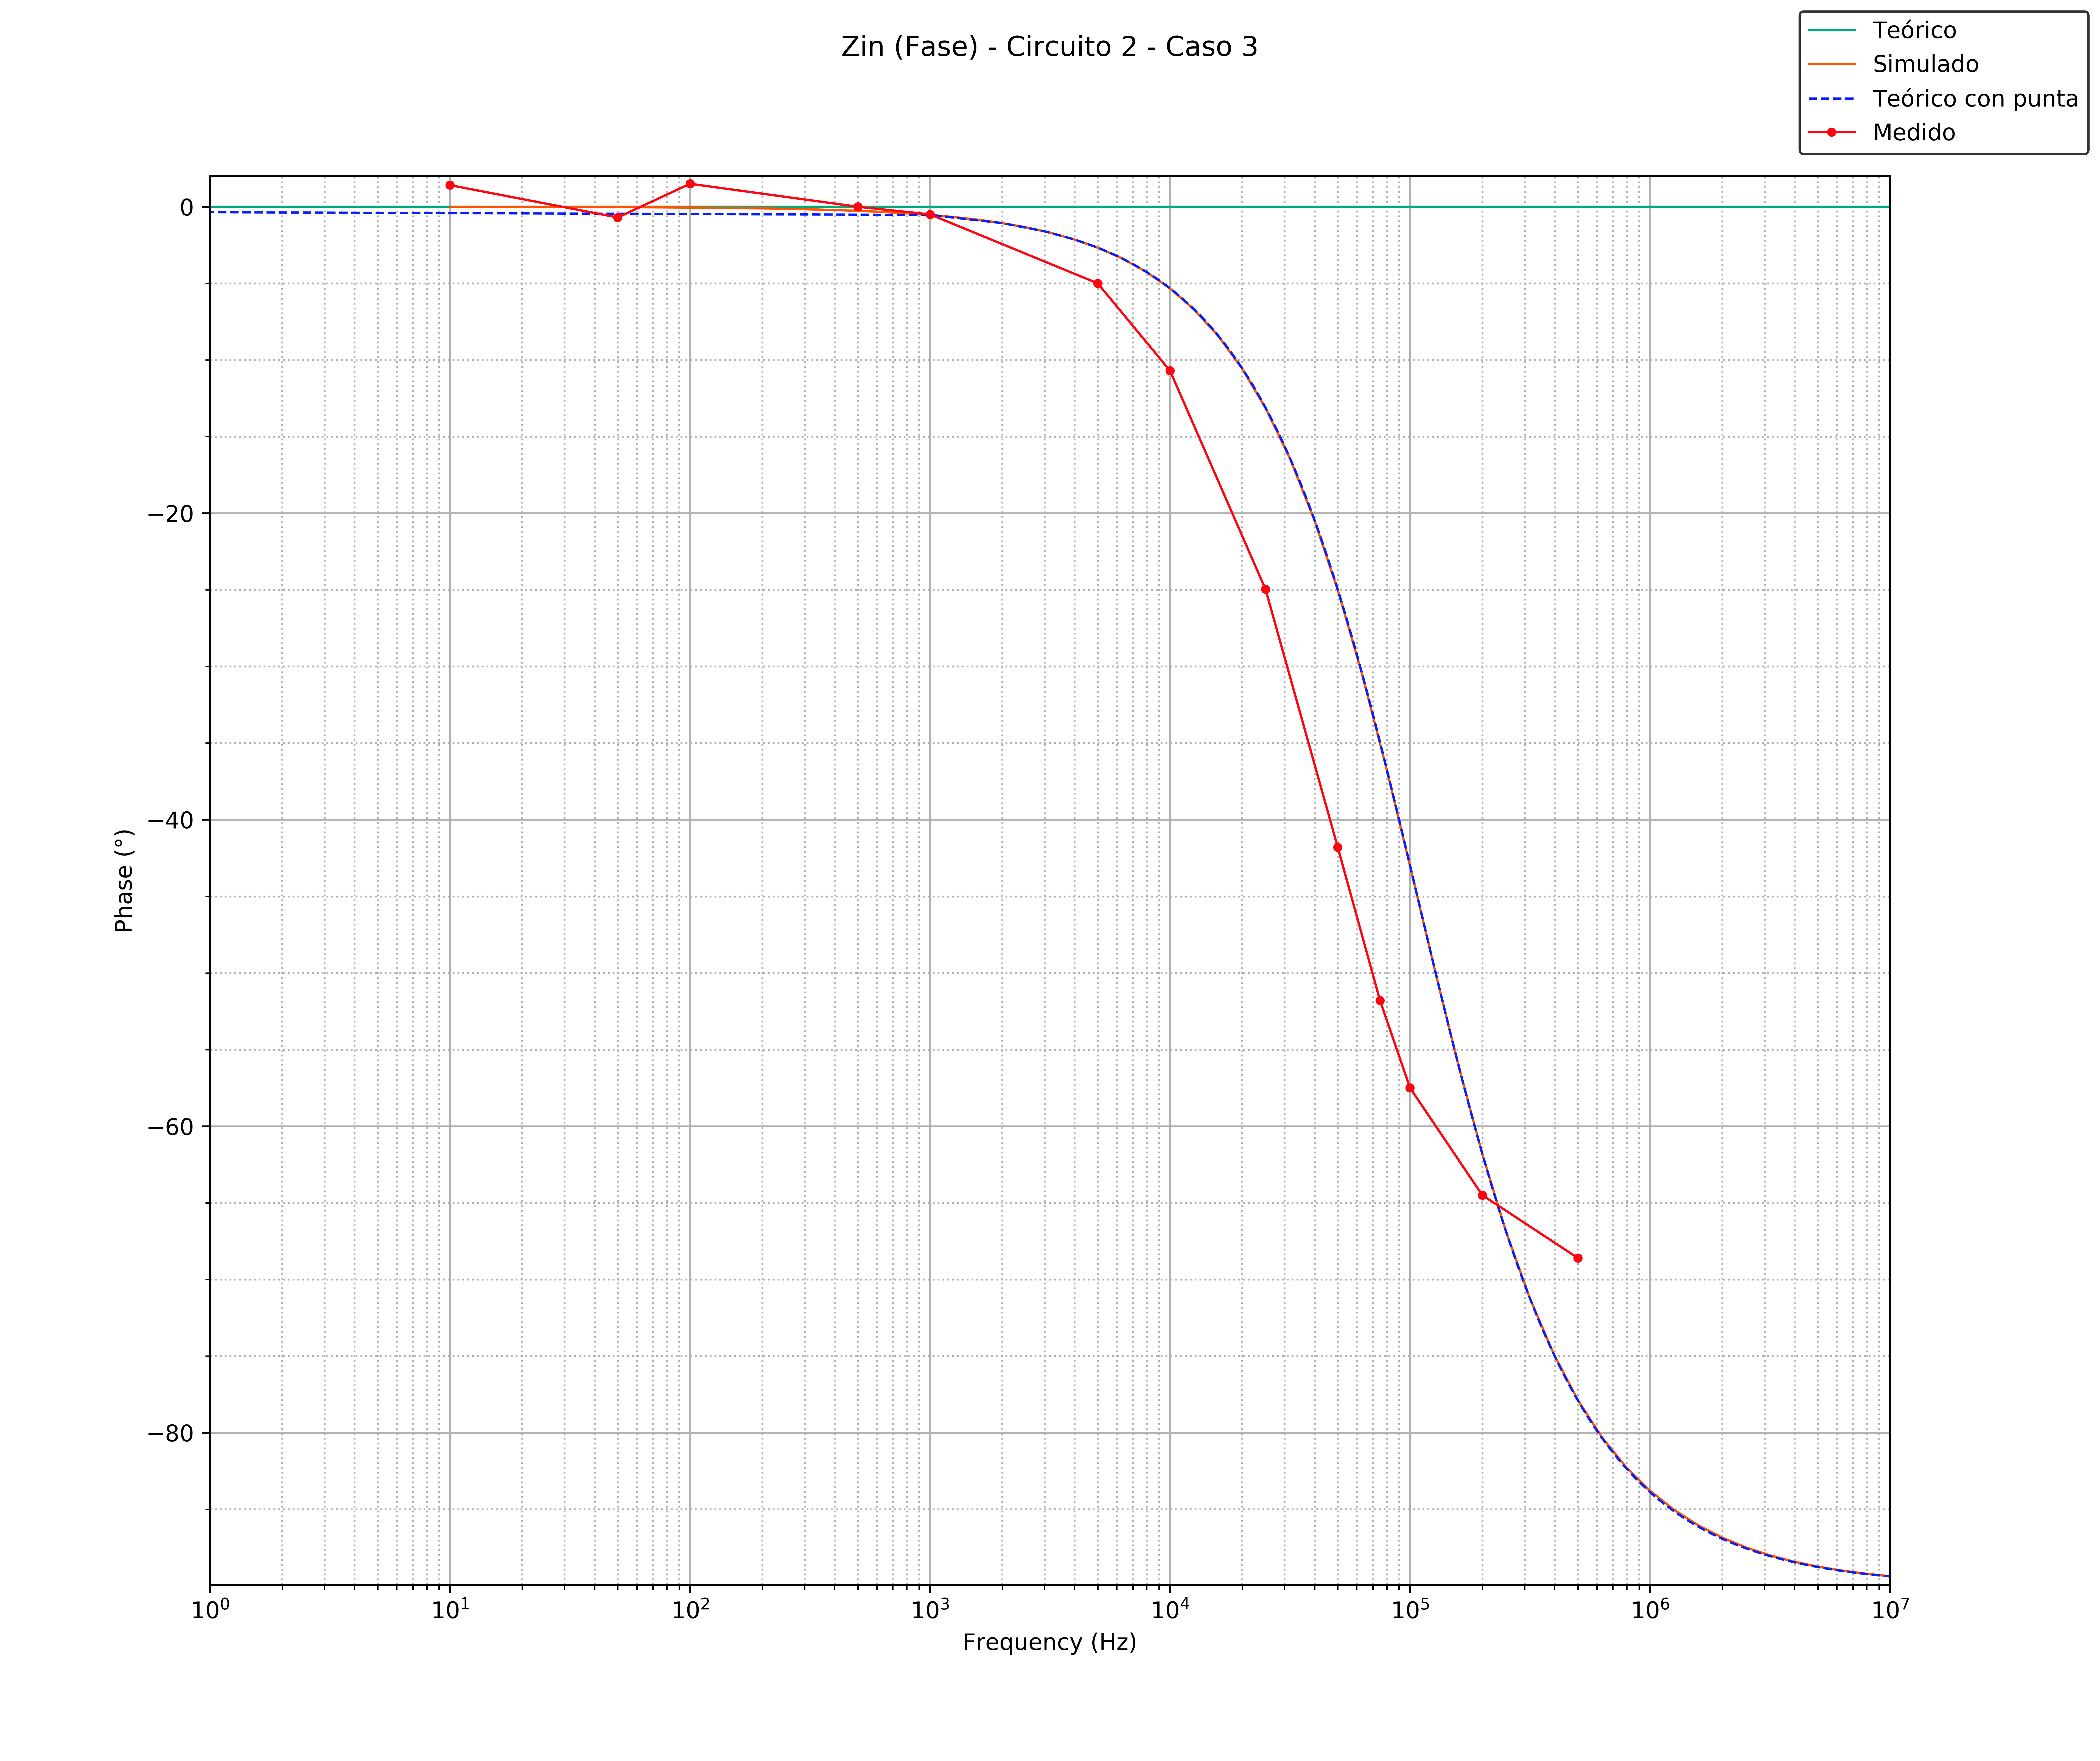
\includegraphics[width=10cm,height=10cm,keepaspectratio]{../EJ1/00GRAFICOS/c2c3/c2c3zinFASE.png}
	\caption{Configuración no inversora - Caso 3 - Fase de $V_{out}/V_{in}$}
	\label{c2c3zinP}
\end{figure}




















%%%%%%%%%%%%%%%%%%%%%%%%%%%%%%%%%%
Circuito 1 Vo/Vi CASO 1
\begin{equation}
- \frac{7000000000000.0}{2088908.62808113 s + 700131250000.0}
\end{equation}

Circuito 1 Vo/Vi CASO 2
\begin{equation}
- \frac{700000000000.0}{298415.518297304 s + 700018750000.0}
\end{equation}

Circuito 1 Vo/Vi CASO3
\begin{equation}
- \frac{7000000000000.0}{11936620.7318921 s + 70000750000000.0}
\end{equation}
%%%%%%%%%%%%%%%%%%%%%%%%%%%%%%%%%

CIRCUITO 1 ZIN
caso1
\begin{equation}
\frac{437.676093502712 s + 280027500.0}{0.0159154943091895 s + 112001.0}
\end{equation}
CON PUNTA:
\begin{equation}
\frac{1.0 \left(3.64730077918927 \cdot 10^{20} s + 2.3335625 \cdot 10^{26}\right)}{4376760935.02712 s^{2} + 1.60996599321165 \cdot 10^{16} s + 9.33575022916667 \cdot 10^{22}}
\end{equation}

inverter: Zin caso2=
\begin{equation}
\frac{79.5774715459477 s + 280005000.0}{0.0159154943091895 s + 112001.0}
\end{equation}
CON PUNTA:
\begin{equation}
\frac{1.0 \left(6.63145596216231 \cdot 10^{19} s + 2.333375 \cdot 10^{26}\right)}{795774715.459477 s^{2} + 1.60695933802868 \cdot 10^{16} s + 9.33575004166667 \cdot 10^{22}}
\end{equation}

inverter: Zin caso3=
\begin{equation}
\frac{437.676093502712 s + 2800027500.0}{0.0159154943091895 s + 112001.0}
\end{equation}
CON PUNTA:
\begin{equation}
\frac{1.0 \left(3.64730077918927 \cdot 10^{20} s + 2.33335625 \cdot 10^{27}\right)}{4376760935.02712 s^{2} + 4.12996599321165 \cdot 10^{16} s + 9.35675022916667 \cdot 10^{22}}
\end{equation}
%%%%%%%%%%%%%%%%%%%%%%%%%%%%%%%%%%%%%%%
circ2 caso1 vovi:
\begin{equation}
\frac{2200000000.0}{437.676093502712 s + 250027500.0}
\end{equation}

circ2 caso2 vovi:
\begin{equation}
\frac{400000000.0}{79.5774715459477 s + 250005000.0}
\end{equation}

circ2 caso3 vovi:
\begin{equation}
\frac{2200000000.0}{437.676093502712 s + 2500027500.0}
\end{equation}

%%%%%%%%%%%%%%%%%%%%%%%%%%%%%%%%%%%%%%%
CIRCUITO 2
ZIN
caso1
\begin{equation}
Zin = R3 + R4 = 12.5kohm
\end{equation}
CON PUNTA:
\begin{equation}
\frac{1.0 \left(1.34287121997052 \cdot 10^{38} s - 8.4366609366572 \cdot 10^{43}\right)}{1.61144546396462 \cdot 10^{27} s^{2} + 9.74400011449559 \cdot 10^{33} s - 6.75776541020242 \cdot 10^{39}}
\end{equation}

NONinverter: Zin caso2=
\begin{equation}
12.5kohm
\end{equation}
CON PUNTA:
\begin{equation}
\frac{1.0 \left(3.35718845716807 \cdot 10^{36} s - 2.10935402480826 \cdot 10^{43}\right)}{4.02862614860169 \cdot 10^{25} s^{2} + 1.57883363155109 \cdot 10^{31} s - 1.68959257386991 \cdot 10^{39}}
\end{equation}

NONinverter: Zin caso3=
\begin{equation}
125kohm
\end{equation}
CON PUNTA:
\begin{equation}
\frac{1.0 \left(1.34287632288 \cdot 10^{39} s - 8.43749203068526 \cdot 10^{46}\right)}{1.611451587456 \cdot 10^{28} s^{2} - 1.00162173591756 \cdot 10^{36} s - 6.83436854484906 \cdot 10^{41}}
\end{equation}

%%%%%%%%%%%%%%%%%%%%%%%%%%%%%%%%%%%%%
%%%%%%%%%%%%%%%%%%%%%%%%%%%%%%%%%%%
%%%%%%%%%%%%%%%%%%%%%%%%%%%%%%%%%%%
zin circuito1 caso1 teorica:
\begin{equation}
\frac{1.30885711543124 \cdot 10^{16} s - 3.6842622243421 \cdot 10^{27}}{2748284324476.07 s - 7.73606889861856 \cdot 10^{23}}
\end{equation}

zin circuito1 caso2 teorico:
\begin{equation}
\frac{2500.0 \left(1202441.0 s - 5.38729407038047 \cdot 10^{15}\right)}{802241.0 s - 3.59439807358207 \cdot 10^{15}}
\end{equation}

zin circ1 caso2 teo BIEN:
\begin{equation}
\frac{1.868890907484 \cdot 10^{15} s - 5.26102936560593 \cdot 10^{25}}{498752424613.223 s - 1.404061747493 \cdot 10^{22}}
\end{equation}

zin circ1 caso3 teo:
\begin{equation}
\frac{7.49205761516139 \cdot 10^{17} s - 2.10926458373408 \cdot 10^{28}}{27480414888480.5 s - 7.73677133618684 \cdot 10^{23}}
\end{equation}


zin circ2 caso1 teo:
\begin{equation}
\frac{1.61144546396462 \cdot 10^{20} s - 1.01239931239886 \cdot 10^{26}}{1.28915648576337 \cdot 10^{16} s - 8.09919449911891 \cdot 10^{21}}
\end{equation}

zin circ2 caso2 teo:
\begin{equation}
\frac{4.02862614860169 \cdot 10^{18} s - 2.53122482976991 \cdot 10^{25}}{322290120536142.0 s - 2.02497986381413 \cdot 10^{21}}
\end{equation}


zin circ2 caso3 teo:
\begin{equation}
\frac{1.611451587456 \cdot 10^{21} s - 1.01249904368223 \cdot 10^{29}}{1.28916241588535 \cdot 10^{16} s - 8.09999234945065 \cdot 10^{23}}
\end{equation}



\section*{Ejercicio 2}
\subsection{Análisis teórico}
El circuito a analizar consiste, a grandes rasgos, en un amplificador no inversor.
Para su estudio teórico se tomarán dos modelos, donde, en primer lugar, se considerará al amplificador operacional en su versión ideal, para luego introducir no idealidades en su impedancia de entrada, salida y en la ganancia del mismo.
Los valores de las resistencias a utilizar fueron reemplazados por su valor comercial más cercano, resultando en que el circuito a analizar sea el de la figura \ref{fig:initial_circuit}.
\begin{figure}[H]
    \begin{minipage}{\textwidth}
        \centering
        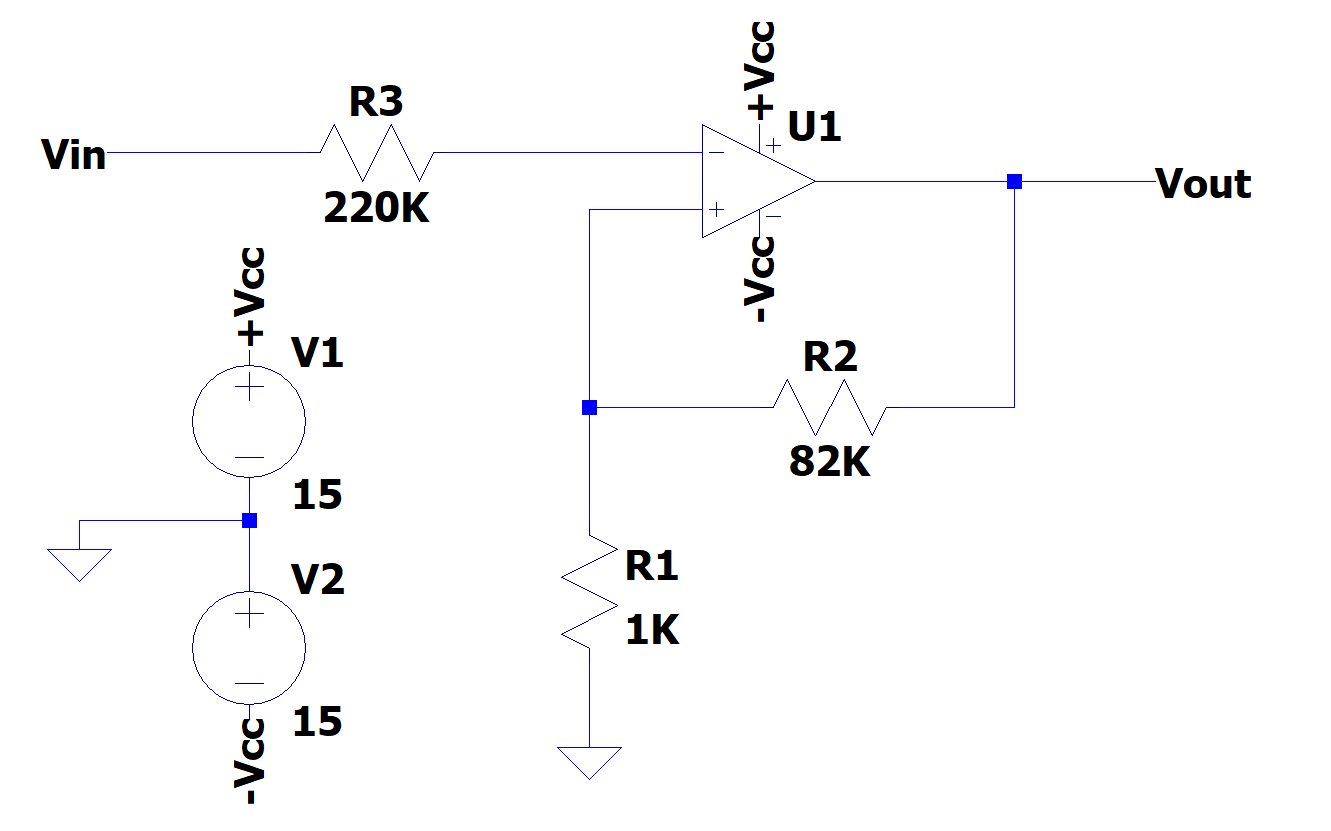
\includegraphics[width=\textwidth]{../EJ2/recursos_para_el_informe/circuito_a_analizar_ideal}
        \caption{Circuito a analizar.}
        \label{fig:initial_circuit}
    \end{minipage}\hfill
\end{figure}

Ha de prestarse especial atención al nodo de la entrada no inversora del operacional.
El mismo se encuentra a alta impedancia, ya que a su izquierda tiene la resistencia de $220K\Omega$, y a su derecha la impedancia interna del operacional (también alta).
Esto lo convierte esencialmente en una antena, susceptible a captar señales de su entorno y, dado que está conectado a un circuito con una alta amplificación (cercana a los 40dB), amplificar esta señal parásita a la salida.\par
Este problema fue afrontado al realizar las mediciones con el operacional LM833 (uno de los dos pedidos), y se ofreció una solución al mismo que será detallada más adelante en las conclusiones del ejercicio.
Luego, para el segundo operacional (NE5534), se decidió reemplazar a la misma por una de inferior valor, y se tomó como criterio hacer uso de la resistencia óptima para la compensación de las corrientes de bias.
El valor para tal resistencia se obtiene de tomar el paralelo entre la resistencia de entrada al sistema, y la de feedback:
\begin{equation}
    R_3' = \frac{R_1 \cdot R_2}{R_1 + R_2} = \frac{1K\Omega \cdot 82K\Omega}{1K\Omega + 82K\Omega} \approx 1K\Omega
\end{equation}

\subsubsection{Modelo ideal}
La primer aproximación al comportamiento del circuito se realizará considerando al amplificador operacional como un componente ideal, es decir, $Av = \inf$, $Z_{in_{opamp}} = \inf$, $Z_{out_{opamp}} = 0$.
De esta manera, sin importar el modelo de operacional utilizado, se tiene que:
\begin{equation}
    \label{eq:ideal_gain}
    \frac{v_{out}}{v_{in}} = 1 + \frac{R_2}{R_1} = 1 + \frac{82 K\Omega}{1 K\Omega} = 83 \implies 38,38 dB
\end{equation}

Se desprende también, de las condiciones de idealidad impuestas, que la impedancia de entrada del circuito será infinita.


\subsubsection{Modelo con impedancia de entrada, salida, y ganancia finita}
Para la resolución del circuito con las consideraciones ya mencionadas, es necesario ahora especificar qué datos serán utilizados para los cálculos.
Los mismos fueron obtenidos de las correspondientes datasheets 
\footnote{Datasheet para operacional LM833: https://www.ti.com/lit/ds/symlink/lm833.pdf \\Datasheet para operacional NE5534: https://www.onsemi.com/pub/Collateral/NE5534-D.PDF}, 
y se presentan en el cuadro \ref{tab:parameters_for_equations}.
\begin{table}[H]
    \label{tab:parameters_for_equations}
    \centering
    \begin{tabular}{|l|lllll|}
        \hline
        \textbf{\begin{tabular}[c]{@{}l@{}}Modelo de operacional\end{tabular}} & \textbf{\begin{tabular}[c]{@{}l@{}}$f_0$ (Hz)\end{tabular}} & \textbf{\begin{tabular}[c]{@{}l@{}}$A_0$ \end{tabular}} & \textbf{$r_{in_{opamp}}(K\Omega)$} & \textbf{$r_{out_{opamp}}(\Omega)$} & \textbf{$C_{in_{opamp}}(pF)$} \\ \hline
        \textbf{LM833}                                                         & $16 \cdot 10^3$                                             & $1000$                                                  & $175$                              & $37$                               & $12$                          \\
        \textbf{NE5534}                                                        & $100$                                                       & $10 \cdot 10^5$                                         & $100$                              & $0,3$                              & -                             \\ \hline
        \end{tabular}
    \caption{Parámetros para cálculo de circuito no ideal.}
\end{table}

Se modelizará al operacional mediante el circuito \ref{fig:non_ideal_circuit}.
\begin{figure}[H]
    \begin{minipage}{\textwidth}
        \centering
        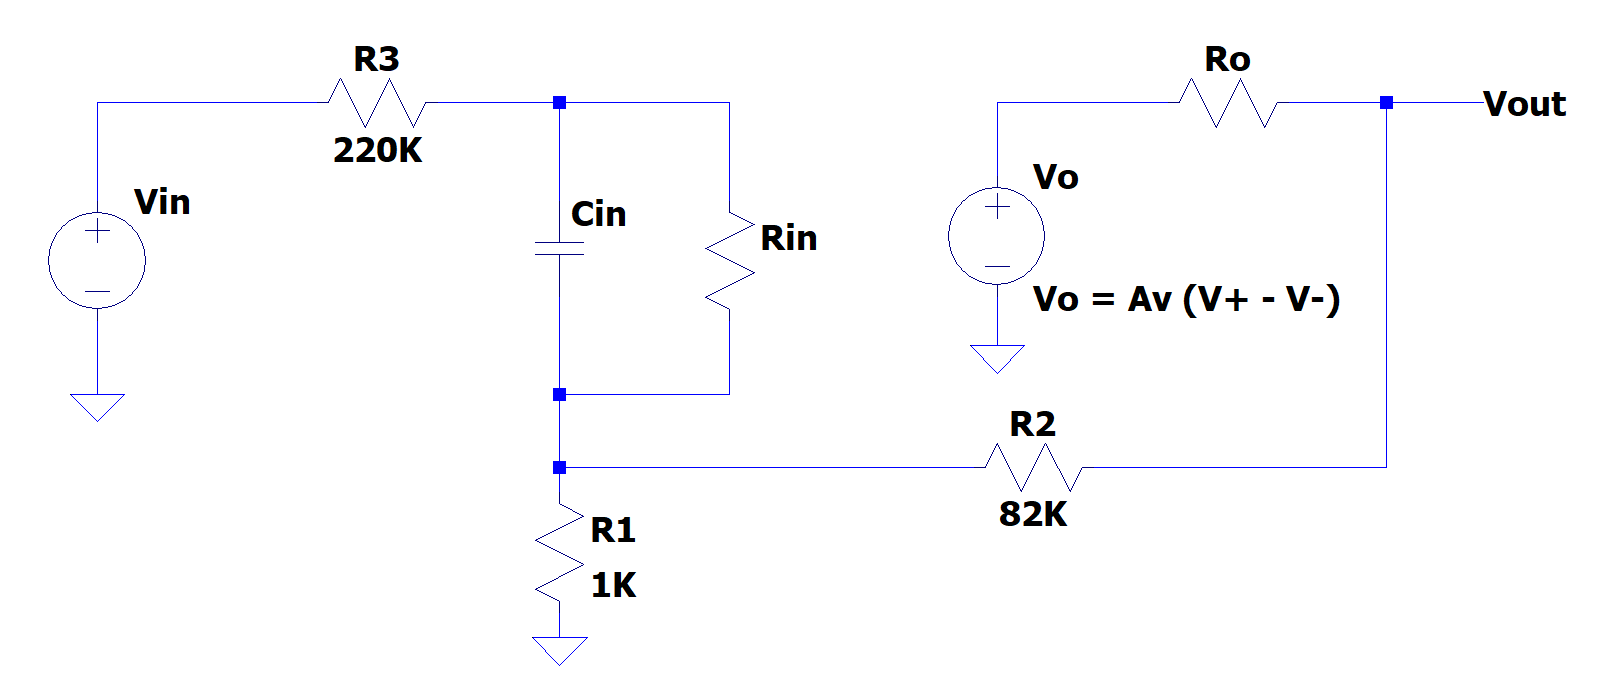
\includegraphics[width=\textwidth]{../EJ2/recursos_para_el_informe/circuito_a_analizar_no_ideal}
        \caption{Circuito a analizar.}
        \label{fig:non_ideal_circuit}
    \end{minipage}\hfill
\end{figure}

Se entiende al circuito como dos mallas cuyas ecuaciones son las descriptas en \ref{eq:system_meshes}, que se extraen del circuito \ref{fig:meshes_circuit}.
\begin{figure}[H]
    \begin{minipage}{\textwidth}
        \centering
        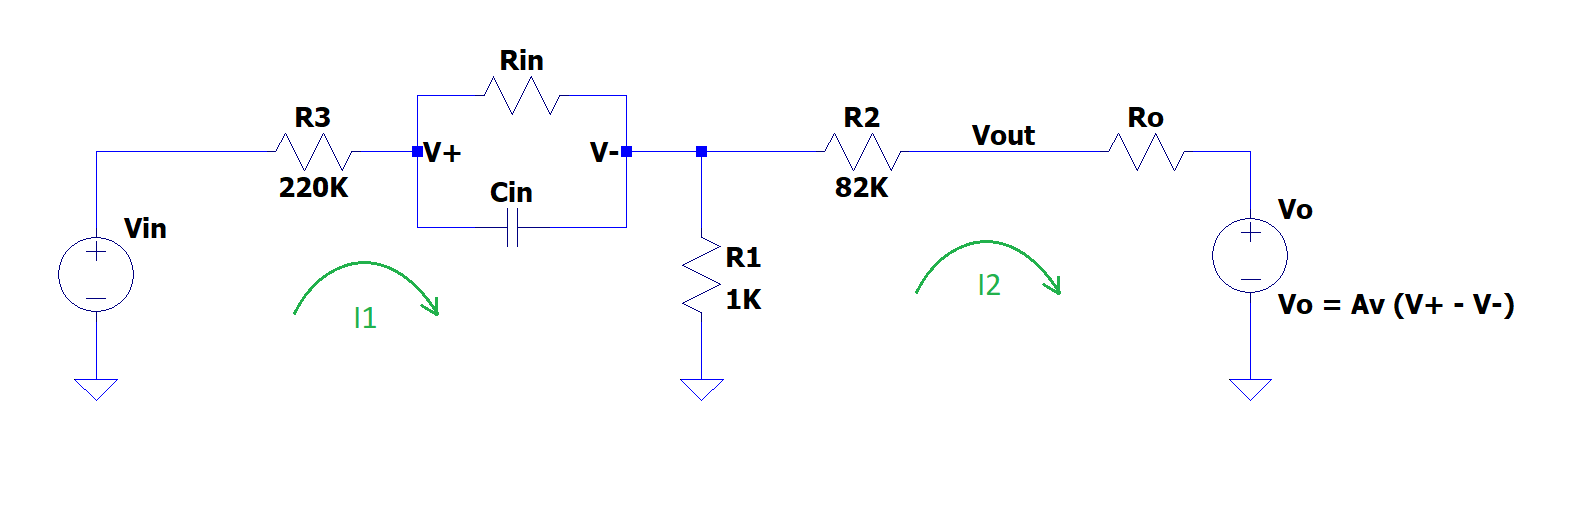
\includegraphics[width=\textwidth]{../EJ2/recursos_para_el_informe/circuito_mallas}
        \caption{Circuito a analizar.}
        \label{fig:meshes_circuit}
    \end{minipage}\hfill
\end{figure}

\begin{align}
    \label{eq:system_meshes}
    &v_{in} - i_1 \cdot R_3 - i_1 \cdot Z_{in} - \left(i_1 - i_2\right) \cdot R_1 = 0 \\
    &-\left(i_2 - i_1\right) \cdot R_1 - i_2 \cdot R_2 - I_2 \cdot R_0 - v_o = 0 \\
    &v_o = \left(v^+ - v^-\right) \cdot A_v \\
    &v^+ = v_{in} - i_1 \cdot R_3 \\
    &v^- = v_{in} - i_1 \cdot R_3 - i_1 \cdot Z_{in} \\
    &Z_{in} = \frac{R_{in}}{R_{in} \cdot C_{in} \cdot s + 1} \label{eq:zin} \\
    &A_v = \frac{A_0}{1+\frac{s}{\omega_p}}
\end{align}

Resolviendo para $i_2$ se obtiene que:
\begin{equation}
    i_2 = v_{in} \cdot \frac{R_1 - A_v \cdot Z_{in}}{R1 \cdot \left(A_v \cdot Z_{in} - R_1\right) + \left(R_3 + Z_{in} + R_1\right) \cdot \left(R_1 + R_2 + R_o\right)}
    \label{eq:i2}
\end{equation}

Y luego se expresan $v_{out}$ e $i_1$ en función de $i_2$ como:
\begin{align}
    \label{eq:i1_and_vout}
    &i_1 = \frac{v_{in} + i_2 \cdot R_1}{R_3 + Z_{in} + R_1} \\
    &v_{out} = v_{in} \cdot \frac{R_1}{R_3 + Z_{in} + R_1} + i_2 \cdot \frac{R_1^2}{R_3 + Z_{in} + R_1} + i_2 \cdot R_1 - i_2 \cdot R_2
\end{align}

\subsubsection{Ecuaciones teóricas para el LM833}
De los resultados obtenidos en \ref{eq:i1_and_vout}, y con los datos de la tabla \ref{tab:parameters_for_equations}, se tiene:
\begin{align}
    & \frac{v_{out}^{LM833}}{v_{in}} = \frac{1,11 \cdot 10^{-4} \cdot s^{4} + 1,105 \cdot 10^{3} \cdot s^{3} + 3,698 \cdot 10^{13} \cdot s^{2} + 3,471b\cdot 10^{20} \cdot s + 2,692 \cdot 10^{26}}
    {s^{4} + 1,034 \cdot 10^{7} s^{3} + 1,678 \cdot 10^{13} \cdot s^{2} + 1,203 \cdot 10^{19} s + 3,948 \cdot 10^{24}} \label{eq:LM833_transfer_fun} \\
    & Z_{in}^{LM833} = \label{eq:LM833_in_impedance} \\
\end{align}
\todo[inline]{NE5534 Transfer function}

\subsubsection{Ecuaciones teóricas para el NE5534}
De los resultados obtenidos en \ref{eq:i1_and_vout}, y con los datos de la tabla \ref{tab:parameters_for_equations}, se tiene:
\begin{align}
    & \frac{v_{out}^{NE5534}}{v_{in}} = \label{eq:NE5534_transfer_fun} \\
    & Z_{in}^{NE5534} = \label{eq:NE5534_in_impedance}
\end{align}
\todo[inline]{LM833 Input inpedance}
\todo[inline]{NE5534 Input inpedance}


\subsection{Simulación}
Para el análisis de los circuitos mediante herramientas de simulación se empleó el programa LTspice, para el cual se realizaron dos esquemáticos, uno para cada uno de los operacionales.
En ambos casos, se simuló la respuesta en frecuencia utilizando la función AC Analysis, y se obtuvieron así los diagramas de bode e impedancia de entrada del sistema, seleccionando las variables pertinentes a observar en el graficador.
A continuación se presentan los circuitos utilizados para tal fin:
\missingfigure{Circuit in LTspice for LM833}
\missingfigure{Circuit in LTspice for NE5534}

\section{Ejercicio 3}
\subsection{Intruducci\'on}
Las corrientes de  BIAS y la tensi\'on de \textit{Input Offset} 
% Defino el tipo de documento
\documentclass[a4paper, 11pts]{article}

% Paquetes usados para el informe
\usepackage[utf8]{inputenc}
\usepackage[spanish]{babel}	
\usepackage{float}
\usepackage{amsmath}

% Estilo del documento
\renewcommand*\familydefault{\sfdefault} 		% Sans Serif as default font
\usepackage[a4paper, 					% Page Layout
                     %showframe,				% This shows the frame
                     includehead,
                     footskip=7mm, headsep=6mm, headheight=4.8mm,
                     top=25mm, bottom=25mm, left=25mm, right=25mm]{geometry}

\setlength{\parindent}{0cm}

\begin{document}

\section{Ejercicio 4: Derivador e Integrador}
En la presente secci\'on se estudiar\'an los circuitos derivador e integrador implementados con amplificador operacionales, analizando su comportamiento, rango de funcionamiento y cualidades o defectos. Adem\'as se presentar\'a un circuito para cada uno de ellos con modificaciones con el fin de mejorar su funcionamiento y se comparar\'an los resultados entre ellos.

Para cada uno de los circuitos, se realiza un an\'alisis te\'orico del mismo y luego se presentan las mediciones y los resultados de las mismas, contrastando o comparando lo observado en la pr\'actica, la simulaci\'on y la teor\'ia.

Adem\'as, todo an\'alisis te\'orico se realiza teniendo en cuenta que los circuitos son armados empleando una resistencia $R = 5k \Omega$, un capacitor $C = 20nF$ y un amplificador operacional LM833 cuyos par\'ametros son:
\begin{itemize}
	\item $A_{vol} = 100000$
	\item $f_p = 150Hz$
	\item $GBP = 15MHz$
	\item $SR = 7 \frac{V}{\mu s}$
	\item $r_{id} = 175k \Omega$
	\item $Z_o = 37 \Omega$
\end{itemize}


	\subsection{Circuito derivador}
 
\subsubsection{An\'alisis Te\'orico}

\begin{figure}[H]
	\centering
	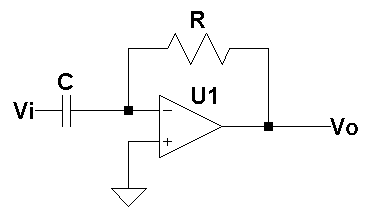
\includegraphics[scale=0.8]{Recursos/Derivador/Circuito_derivador.png}
	\caption{Circuito derivador}
	\label{fig:circuito_derivador}
\end{figure}

\paragraph*{Funci\'on transferencia en condiciones ideales}se busca la funci\'on de transferencia del circuito bajo condiciones ideales, esto es, asumiendo que el amplificador operacional no tiene variaci\'on en su ganancia de lazo abierto con la frecuencia y que la misma tiende a infinito, $A_{vol} \to \infty$. En este marco de idealidad, las impedancias de entrada y salida del amplificador operacional son $Z_{in} \to \infty$ y $r_o = 0$. Para este c\'alculo se conoce la ganancia ideal de un amplificador inversor y se asume al mismo un sistema LTI, causal y bibo-estable.

\begin{equation}
	H(s) = \frac{V_o}{V_i} = \frac{-R}{ \frac{1}{s \cdot C}} = -s \cdot R  \cdot C
	= -\frac{s}{10000}
	\label{eq:derivador_transfer_ideal}
\end{equation}

Se puede observar que por la propiedad de la derivada para transformada de Laplace, multiplicar por la variable $s$ en tal dominio, implica derivar la señal en el dominio temporal, de forma tal que se puede llegar:

\begin{equation*}
	V_o(s) = V_i(s) \cdot H(s) = V_i(s) \cdot -sRC \Rightarrow
	Vo(t) = -RC \cdot \frac{\delta V_i(t)}{\delta t}
\end{equation*}

Otra observaci\'on sobre la funci\'on de transferencia ideal, es que para frecuencias altas, 
seg\'un la magnitud de la se\~nal de entrada, se puede producir la saturaci\'on del amplificador
operacional pues la ganancia es muy elevada y la salida supera el valor de la fuente de 
alimentaci\'on del circuito. Por otro lado, el sistema descripto por dicha funci\'on de 
transferencia ideal, no es bibo-estable como se asumi\'o desde el principio. 
Esto se obtiene del hecho de que la antitransformada de la funci\'on transferencia, es decir la respuesta impulsiva, 
es la derivada del delta de dirac. Ergo, para se\~nales acotadas en la entrada, la operaci\'on de derivar
puede dar como resultado, en algunos casos, una se\~nal de salida no acotada.

%TODO Agregar diagrama de polos y ceros aca!

\paragraph*{Funci\'on transferencia con $A_{vol}$ finito}se considera que $A_{vol}$ es finito con lo cual se lo debe tener en cuenta, y para llegar a la funci\'on transferencia se plantea por un lado la superposici\'on de las tensiones sobre las entradas del amplificador operacional y luego la expresi\'on de salida del mismo para obtener:

\begin{equation*}
	v^{-} = \frac{V_i \cdot R}{\frac{1}{sC} + R} + \frac{V_o \cdot \frac{1}{sC}}{\frac{1}{sC} + R}
	= \frac{V_i \cdot s \cdot R \cdot C + V_o}{1 + s \cdot R \cdot C}
\end{equation*}

\begin{align*}
	V_o = (v^{+} - v^{-}) \cdot A_{vol}
	= - \frac{V_i \cdot s \cdot R \cdot C + V_o}{1 + s \cdot R \cdot C} \cdot A_{vol} \\
	V_o \cdot \left[ 1 + \frac{A_{vol}}{1 + s \cdot R \cdot C} \right]
	= - \frac{V_i \cdot s \cdot R \cdot C \cdot A_{vol}}{1 + s \cdot R \cdot C}
\end{align*}
\begin{equation}
	H(s) = \frac{V_o(s)}{V_i(s)} = \frac{\frac{s \cdot A_{vol} \cdot RC}{A_{vol} + 1}}{1 + \frac{s}{\frac{A_{vol} + 1}{R \cdot C}}}
	= - \frac{\frac{s}{2 \pi \cdot 1,591kHz}}{1 + \frac{s}{2 \pi \cdot 159,15MHz}}
	\label{eq:derivador_transfer_avol_finito}
\end{equation}

De esto \'ultimo se puede observar que aparece, a diferencia de antes, un polo adicional que podr\'ia ser despreciado o incluso anulado bajo las condiciones de idealidad previamente analizadas. Es importante destacar de esta nueva funci\'on de transferencia que si se obtiene la frecuencia de corte donde se ubica este polo y limitamos el rango de funcionamiento una decada antes del mismo, podemos considerar condiciones de idealidad tal que el derivador podr\'ia seguir funcionando como tal. Esto tambi\'en se puede ver considerando que, si se llama $\omega_o = \frac{(A_{vol} + 1)}{R \cdot C}$ a la frecuencia angular de corte:
\begin{equation*}
	Si, s << \frac{\omega_o}{10} \Rightarrow 1 >> \frac{s}{\omega_o} \Rightarrow 
	H(s) \approx - \frac{s \cdot A_{vol} \cdot RC}{A_{vol} + 1} \approx
	- s \cdot R \cdot C
\end{equation*}

En primera instancia, este nuevo polo que ha de aparecer establece como se dijo antes un l\'imite superior hasta el
cual puede considerarse que el comportamiento del sistema es ideal. No obstante, por otro lado este aspecto puede resultar beneficioso
en t\'erminos de estabilidad, pues a diferencia de un derivador ideal, a altas frecuencias la ganancia no sigue aumentando.

%TODO Agregar diagrama de polos y ceros aca!

\paragraph*{Funci\'on transferencia con polo dominante} tomando en cuenta el polo dominante 
que el fabricante del amplificador operacional coloca a una baja frecuencia para 
que el ruido se vea atenuado en las altas frecuencias, pues es donde saldr\'ia en contrafase
y producir\'ia una realimentaci\'on positiva. Entonces reemplazado la ecuaci\'on \ref{eq:polo_dominante} 
en la ecuaci\'on \ref{eq:derivador_transfer_avol_finito} y operando:

\begin{equation}
	A_{vol}(\omega) = \frac{A_o}{1 + \frac{s}{\omega_p}}
	\label{eq:polo_dominante}
\end{equation}

\begin{equation}
	H(s) = - \frac{s \cdot A_{o} \cdot R \cdot C}{(1 + s \cdot C \cdot R) \cdot (1 + \frac{s}{\omega_p}) + A_{o}} = - \frac{R \cdot C \cdot A_{o}}{A_{o} + 1} \cdot \frac{s}{1 + s \cdot \frac{1 + \omega_p \cdot RC}{\omega_p \cdot(A_o + 1)} + s^{2} \cdot \frac{RC}{\omega_p \cdot (A_o + 1)}}
\end{equation}

En esta \'ultima condici\'on se puede observar que el circuito se comporta
como un segundo orden por ser de segundo grado en el denominador, 
para lo cual es necesario determinar algunos par\'ametros que permitan
establecer cu\'al es el comportamiento de tal sistema y para ello se 
despejan de las siguientes expresiones los valores de $\xi$ y $\omega_o$.

\begin{equation*}
	\omega_o^{2} = \frac{\omega_p \cdot (A_o + 1)}{RC} \Rightarrow \omega_o = \sqrt{\frac{\omega_p \cdot (A_o + 1)}{RC}}	
\end{equation*}

\begin{equation*}
	\frac{2 \cdot \xi}{\omega_o} = \frac{(1 + \omega_p \cdot R \cdot C)}{\omega_p \cdot(A_o + 1)}
	\Rightarrow \xi = \frac{1}{2} \cdot \frac{1 + \omega_p \cdot R \cdot C}{\sqrt{\omega_p \cdot R \cdot C \cdot (A_o + 1)}}
\end{equation*}

\begin{equation}
	H(s) = - \frac{\frac{s}{2 \pi \cdot 1,591kHz}}
	{1 + s \cdot 11,53 \cdot 10^{-9} + \left( \frac{s}{2 \pi \cdot 154,51kHz} \right)^{2}}
	\label{eq:derivador_transfer_polo_dominante}
\end{equation}

Finalmente, se obtiene que $\omega_o = 970817,81 \frac{1}{s}$ y $\xi = 0,0056357$. Esto \'ultimo indica que la respuesta natural del sistema durante una transici\'on entre estados estables contiene un subamortiguamiento, pero m\'as importante, que los polos son complejos y conjugados donde la frecuencia de corte est\'a en $f_o = 154,51kHz$ y presenta un sobrepico.

Para ubicar a qu\'e frecuencia y con qu\'e magnitud ocurre este pico en la respuesta en frecuencia, se busca el m\'inimo de la funci\'on del denominador de la respuesta en frecuencia en m\'odulo. Vale mencionar que al igual que para los futuros an\'alisis que se hagan, se asume el sistema LTI, causal y bibo-estable con lo que luego se puede evaluar $s = j \omega$ para encontrar la respuesta en frecuencia a partir de la funci\'on transferencia.
Llamando $D(s)$ a la expresi\'on del denominador de la funci\'on transferencia, se busca el m\'inimo del m\'odulo de tal funci\'on.

\begin{equation*}
	D(s) = \left( \frac{s}{\omega_o} \right)^{2} + \frac{2 \cdot \xi}{\omega_o} \cdot s + 1
	\Rightarrow
	D(w) = \frac{j \cdot 2 \cdot \xi \cdot \omega}{\omega_o} + \left( \frac{\omega_o^{2} - \omega^{2}}{\omega_o^{2}} \right)
\end{equation*}

\begin{equation*}
	|D(w)| = \sqrt{\left( \frac{2 \xi \omega}{\omega_o} \right)^{2} + \left( \frac{\omega_o^{2} - \omega^{2}}{\omega_o^{2}} \right)^{2}}
\end{equation*}

\begin{equation}
	\frac{\delta |D(w)|}{\delta w}
	= 0 \Leftrightarrow 2 \cdot \xi^{2} \cdot \omega - \frac{\omega \cdot (\omega_o^{2} - \omega^{2})}{\omega_o^{2}} = 0
	\Leftrightarrow
	\omega = \omega_o \cdot \sqrt{1 - 2 \cdot \xi^{2}}
\end{equation}

Entonces, el pico dentro de la respuesta en frecuencia caracter\'istico de este sistema se puede encontrar, te\'oricamente, en la frecuencia $\omega_{pico} = 970817,8 \cdot \sqrt{1- 2 \cdot (0,0056)^{2}} = 970786,97 \frac{1}{s} \Rightarrow f_{pico} = 154505,54Hz$. Y tendr\'a una magnitud de $|H(f_{pico})| = 8613,05 \Rightarrow |H(f_{pico})|dB = 78,70dB$.

Este comportamiento establece un l\'imite superior al funcionamiento del derivador, pero a diferencia del caso debe
$A_{vol}$ finito, la frecuencia m\'axima es mucho menor. En consecuencia, se observa un comportamiento ideal de derivador hasta
una frecuencia aproximada de $f = 15,45kHz$ donde la fase todav\'ia no empieza a cambiar por los polos complejos.

%TODO Agregar diagrama de polos y ceros aca!

\paragraph*{Impedancia de entrada con $A_{vol}$ finito} en este escenario se analiza la impedancia de entrada del amplificador operacional, considerando las caracter\'isticas reales del modelo equivalente del mismo.

Aplicando una transformaci\'on de fuentes se simplifica el circuito y se deja en evidencia que la fuente de corriente correspondiente a la salida equivale a una impedancia como se muestra en los circuitos de la figura. %TODO Agregar referencia a los circuitos previos
De esta forma se agrupan las impedancias y se encuentra la $Z_{in}$, para ello se llama $Y_r$ y luego $Z_r$ al agrupamiento paralelo de impedancias.

\begin{figure}[H]
\begin{tabular}{c c}
	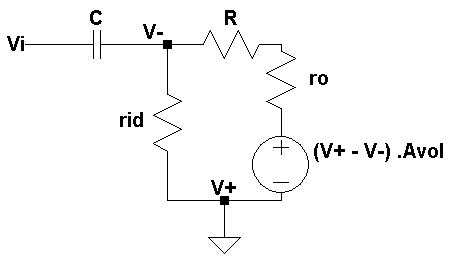
\includegraphics[scale=0.55]{Recursos/Derivador/Circuito_derivador_modelo.png} &
	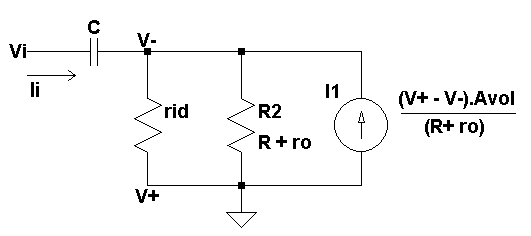
\includegraphics[scale=0.55]{Recursos/Derivador/Circuito_derivador_simplificacion.png}
\end{tabular}
\caption{Circuito derivador con modelo del amplificador y transformaci\'on}
\label{fig:circuito_derivador_impedancia}
\end{figure}

\begin{equation*}
	Y_r = \frac{1}{r_{id}} + \frac{1 + A_{vol}}{R + Z_o} \Rightarrow
	Z_r = \frac{r_{id} \cdot(R + Z_o)}{R + Z_o + r_{id} \cdot(1 + A_{vol})}
\end{equation*}

\begin{equation}
	Z_{in} = \frac{1}{sC} + Z_r
	= \frac{1 + s \cdot \frac{C \cdot r_{id} \cdot (R + Z_o)}{R + Z_o + r_{id} \cdot (1 + A_{vol})}}{s \cdot C}
	\Rightarrow
	Z_{in} = \frac{1 + \frac{s}{2 \pi \cdot 157,98MHz}}{\frac{s}{2 \pi \cdot 7,957MHz}}
	\label{eq:derivador_impedancia_avol_finito}
\end{equation}

En primera instancia, se observa que la impedancia de entrada del circuito derivador no es invariante frente a la frecuencia,
sino que var\'ia, y particularmente para el rango de frecuencias donde $f < 15,79MHz$ la impedancia del mismo, dentro del contexto del an\'alisis, se puede
aproximar a la del capacitor.

\paragraph*{Impedancia de entrada con polo dominante} ahora se adaptan los c\'alculos previos para incluir la apreciaci\'on del polo dominante dentro del an\'alisis de la impedancia de entrada. Operando con la expresi\'on del polo dominante \ref{eq:polo_dominante} se llega a que:

\begin{equation*}
	Z_{in} = \frac{R + Z_o + r_{id} \cdot (A_o + 1 + \frac{s}{\omega_p}) + s \cdot C \cdot r_{id} \cdot (R + Z_o) \cdot (1 + \frac{s}{\omega_p})}{s \cdot C \cdot \left[ (R + Z_o) \cdot (1 + \frac{s}{\omega_p}) + r_{id} \cdot (1 + A_o + \frac{s}{\omega_p}) \right]}
\end{equation*}

\begin{equation*}
	Z_{in} = \frac{1}{s \cdot C} \cdot 
	\frac{1 + s \cdot \frac{R + Z_o + r_{id} + r_{id} \cdot C \cdot \omega_p \cdot(R + Z_o)}{\omega_p \cdot \left[ R + Z_o + r_{id} \cdot (A_o + 1) \right]} + s^{2} \cdot \frac{r_{id} \cdot C \cdot (R + Z_o)}{\omega_p \cdot \left[ R + Z_o + r_{id} \cdot (A_o + 1) \right]}}{1 + s \cdot \frac{R + Z_o + r_{id}}{\omega_p \cdot \left[ R + Z_o + r_{id} \cdot (1 + A_o)\right]}}
\end{equation*}

\begin{align}
	Z_{in} & = \frac{1}{\frac{s}{2 \pi \cdot 7,957MHz}} \cdot
	\frac{1 + s \cdot 11,923 \cdot 10^{-9} + \left(\frac{s}{2 \pi \cdot 153,94kHz}\right)^{2}}{1 + \frac{s}{2 \pi \cdot 14,58MHz}}
	\label{eq:derivador_impedancia_polo_dominante}
\end{align}

Como se puede observar, la impedancia de entrada posee dos ceros complejos y conjugados, ubicados en la frecuencia de corte con $f_o = 153,94kHz$, lo cual establece otra consideración a tener en cuenta con respecto a las limitaciones del circuito, puesto que para esta frecuencia la impedancia de entrada se hace muy chica, produciendose un incremento en el consumo de corriente. Por otro lado, al bajar tanto la impedancia se produce una desadaptaci\'on, es decir, al ser la impedancia de entrada tan peque\~na para esta frecuencia, hay una gran p\'erdida de tensi\'on sobre la resistencia propia de la fuente de la se\~nal.

\paragraph*{Conclusi\'on del an\'alisis} teniendo en cuenta las expresiones finales para caracterizar al circuito derivador con 
la menor idealidad posible, es decir, las ecuaciones \ref{eq:derivador_transfer_polo_dominante} y 
\ref{eq:derivador_impedancia_polo_dominante} se ve como resultado de este an\'alisis que por la forma de la 
funci\'on transferencia el comportamiento derivador se sostiene hasta una frecuencia $f < 154kHz$ aproximadamente, pues hasta esa frecuencia 
se mantiene aproximadamente en $-90^{\circ}$ la fase de la respuesta. No obstante este an\'alisis es estimativo considerando que el valor del $\xi$ es muy cercano a cero puesto
que por no serlo el cambio de fase ocurre antes de dicha frecuencia. Por otro lado, durante este rango de frecuencia la 
 impedancia de entrada est\'a dominada por la del capacitor, con lo cual disminuye hasta que se produce una ca\'ida en el valor 
 de la impedancia y se producen p\'erdidas en la se\~nal que ve el amplificador. Finalmente, el sistema se encuentra subamortiguado, por tanto
 deber\'a poder percibirse tal comportamiento en la respuesta transitoria o en frecuencia del circuito.

\subsubsection{Resultados}
En base a la conclusi\'on del an\'alisis te\'orico realizado, se realizan una serie de simulaciones y mediciones sobre el circuito
para obtener una caracterizaci\'on del mismo y contrastar tales resultados contra lo descripto por lo te\'orico. Vale aclarar que las simulaciones
son graficadas utilizando Monte Carlo para considerar un rango de posibles desviaciones ante la imprecisi\'on de los valores de componentes.

\paragraph*{Respuesta en frecuencia} en las figuras \ref{fig:derivador_bode_modulo} y \ref{fig:derivador_bode_fase} se puede observar
que para el rango de frecuencias donde $f < 100kHz$ aproximadamente, el m\'odulo de la respuesta en frecuencia constrasta con poco error entre
la simulaci\'on, lo te\'orico y la medici\'on. Vale aclarar, que al estar muy subamortiguado el sistema, el cambio de fase se hace muy repentino en torno
a la frecuencia de corte asociada a los polos complejos y conjugados, esto provoca que el comportamiento derivador llegue a operar hasta una alta frecuencia.

Por otro lado, se puede observar que el sobrepico cercano a la frecuencia de corte obtenido te\'oricamente est\'a dentro de los m\'argenes de las aproximaciones
de la simulaci\'on en LTSpice, no obstante, en las mediciones se produce una gran diferencia entre estos valores. Esto \'ultimo se debe a que por un lado la compensaci\'on de un derivador
, como se ver\'a posteriormente, consiste en colocar una resistencia en serie al capacitor y tiene como efecto, entre otros, reducir el subamortiguamiento del sistema. Poniendo a prueba esto \'ultimo,
y considerando que adem\'as de las resistencias par\'asitas por cables y capacitor, aparece la del generador, luego se contrasta contra la simulaci\'on y se ve que ajusta aproximadamente bien. Dicha correcci\'on en
la resistencia en serie del generador para la simulaci\'on corresponde a la figura con el trazo "Simulado R".
Si bien agregando la resistencia del generador justifica la ca\'ida del sobrepico en las mediciones, el valor con el cual se logra ajustar la curva es tomando $R = 25 \Omega $ en serie
 al generador, esto \'ultimo no es muy coherente si se tiene en cuenta que los generadores tienen una impedancia de salida de $R_{g} = 50 \Omega $. Es por esto mismo que se decidi\'o tomar mas mediciones en torno al
 sobrepico con el objetivo de localizarlo con menos error. No obstante, en el proceso de tales mediciones aparecieron algunos inconvenientes que imped\'ian medir correctamente el sobrepico, y se atribuye a tales factores
 el hecho de que el sobrepico obtenido no es realmente el que se produce, sino que el verdadero tiene una magnitud y una frecuencia mayor. Las bases te\'oricas de tal afirmaci\'on salen directo de las conclusiones del an\'alisis
 te\'orico realizado anteriormente, o bien mismo de las mediciones de impedancia de entrada. As\'i, se puede observar que para las frecuencias donde se produce el sobrepico de la transferencia, tambi\'en se produce una ca\'ida abrupta
 en la impedancia de entrada del circuito, y en consecuencia la tensi\'on que ve a la entrada el circuito tambi\'en decrece abruptamente deformandose como se puede observar en la figura \ref{fig:justificacion_derivador}. Se midi\'o las 
 sen\~nales amarilla y verde, es decir, la entrada y salida respectivamente, y se observa que para una entrada que deber\'a de corresponderse con una senoidal, la atenuaci\'on producto de una muy baja impedancia de entrada del orden de $R = 6 \Omega$ 
 no s\'olo produce la saturaci\'on de la salida sino que pierde la forma que esencialmente ten\'ia.
 
 Finalmente, a partir de los $f = 200kHz$ se desv\'ian las curvas te\'orica, medici\'on y simulaci\'on. Esto se atribuye al hecho de que para el orden de estas frecuencias,
 la ganancia produce una saturaci\'on con muy bajas tensiones de salida, sumado a que con altas frecuencias el slew rate limita el rango de operaci\'on. Por lo tanto no se consideran
 apreciables los resultado de mediciones posteriores a $1MHz$ y se puede observar con las desviaciones ya presentadas antes de tal frecuencia.

\begin{figure}[H]
	\centering
	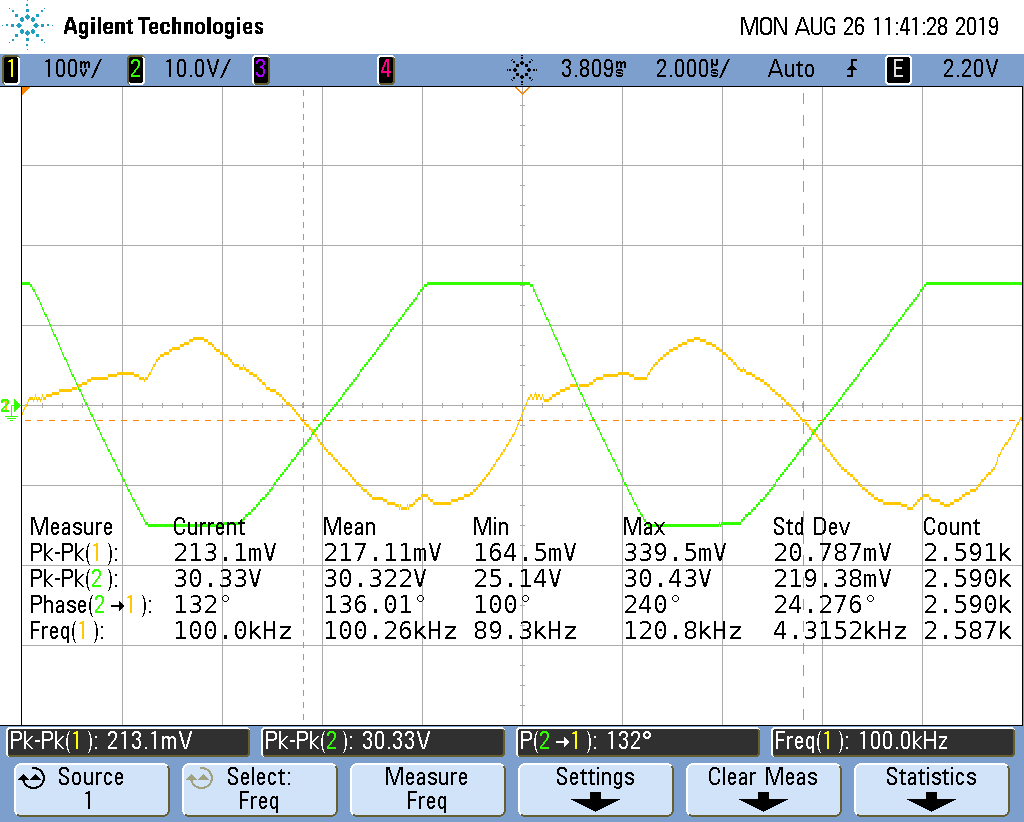
\includegraphics[scale=0.4]{Derivador/Mediciones/Osciloscopio/Justificacion/scope_4.png}
	\caption{Señal amarilla es una entrada senoidal, señal verde es la salida.}
	\label{fig:justificacion_derivador}
\end{figure}

\begin{figure}[H]
	\centering
	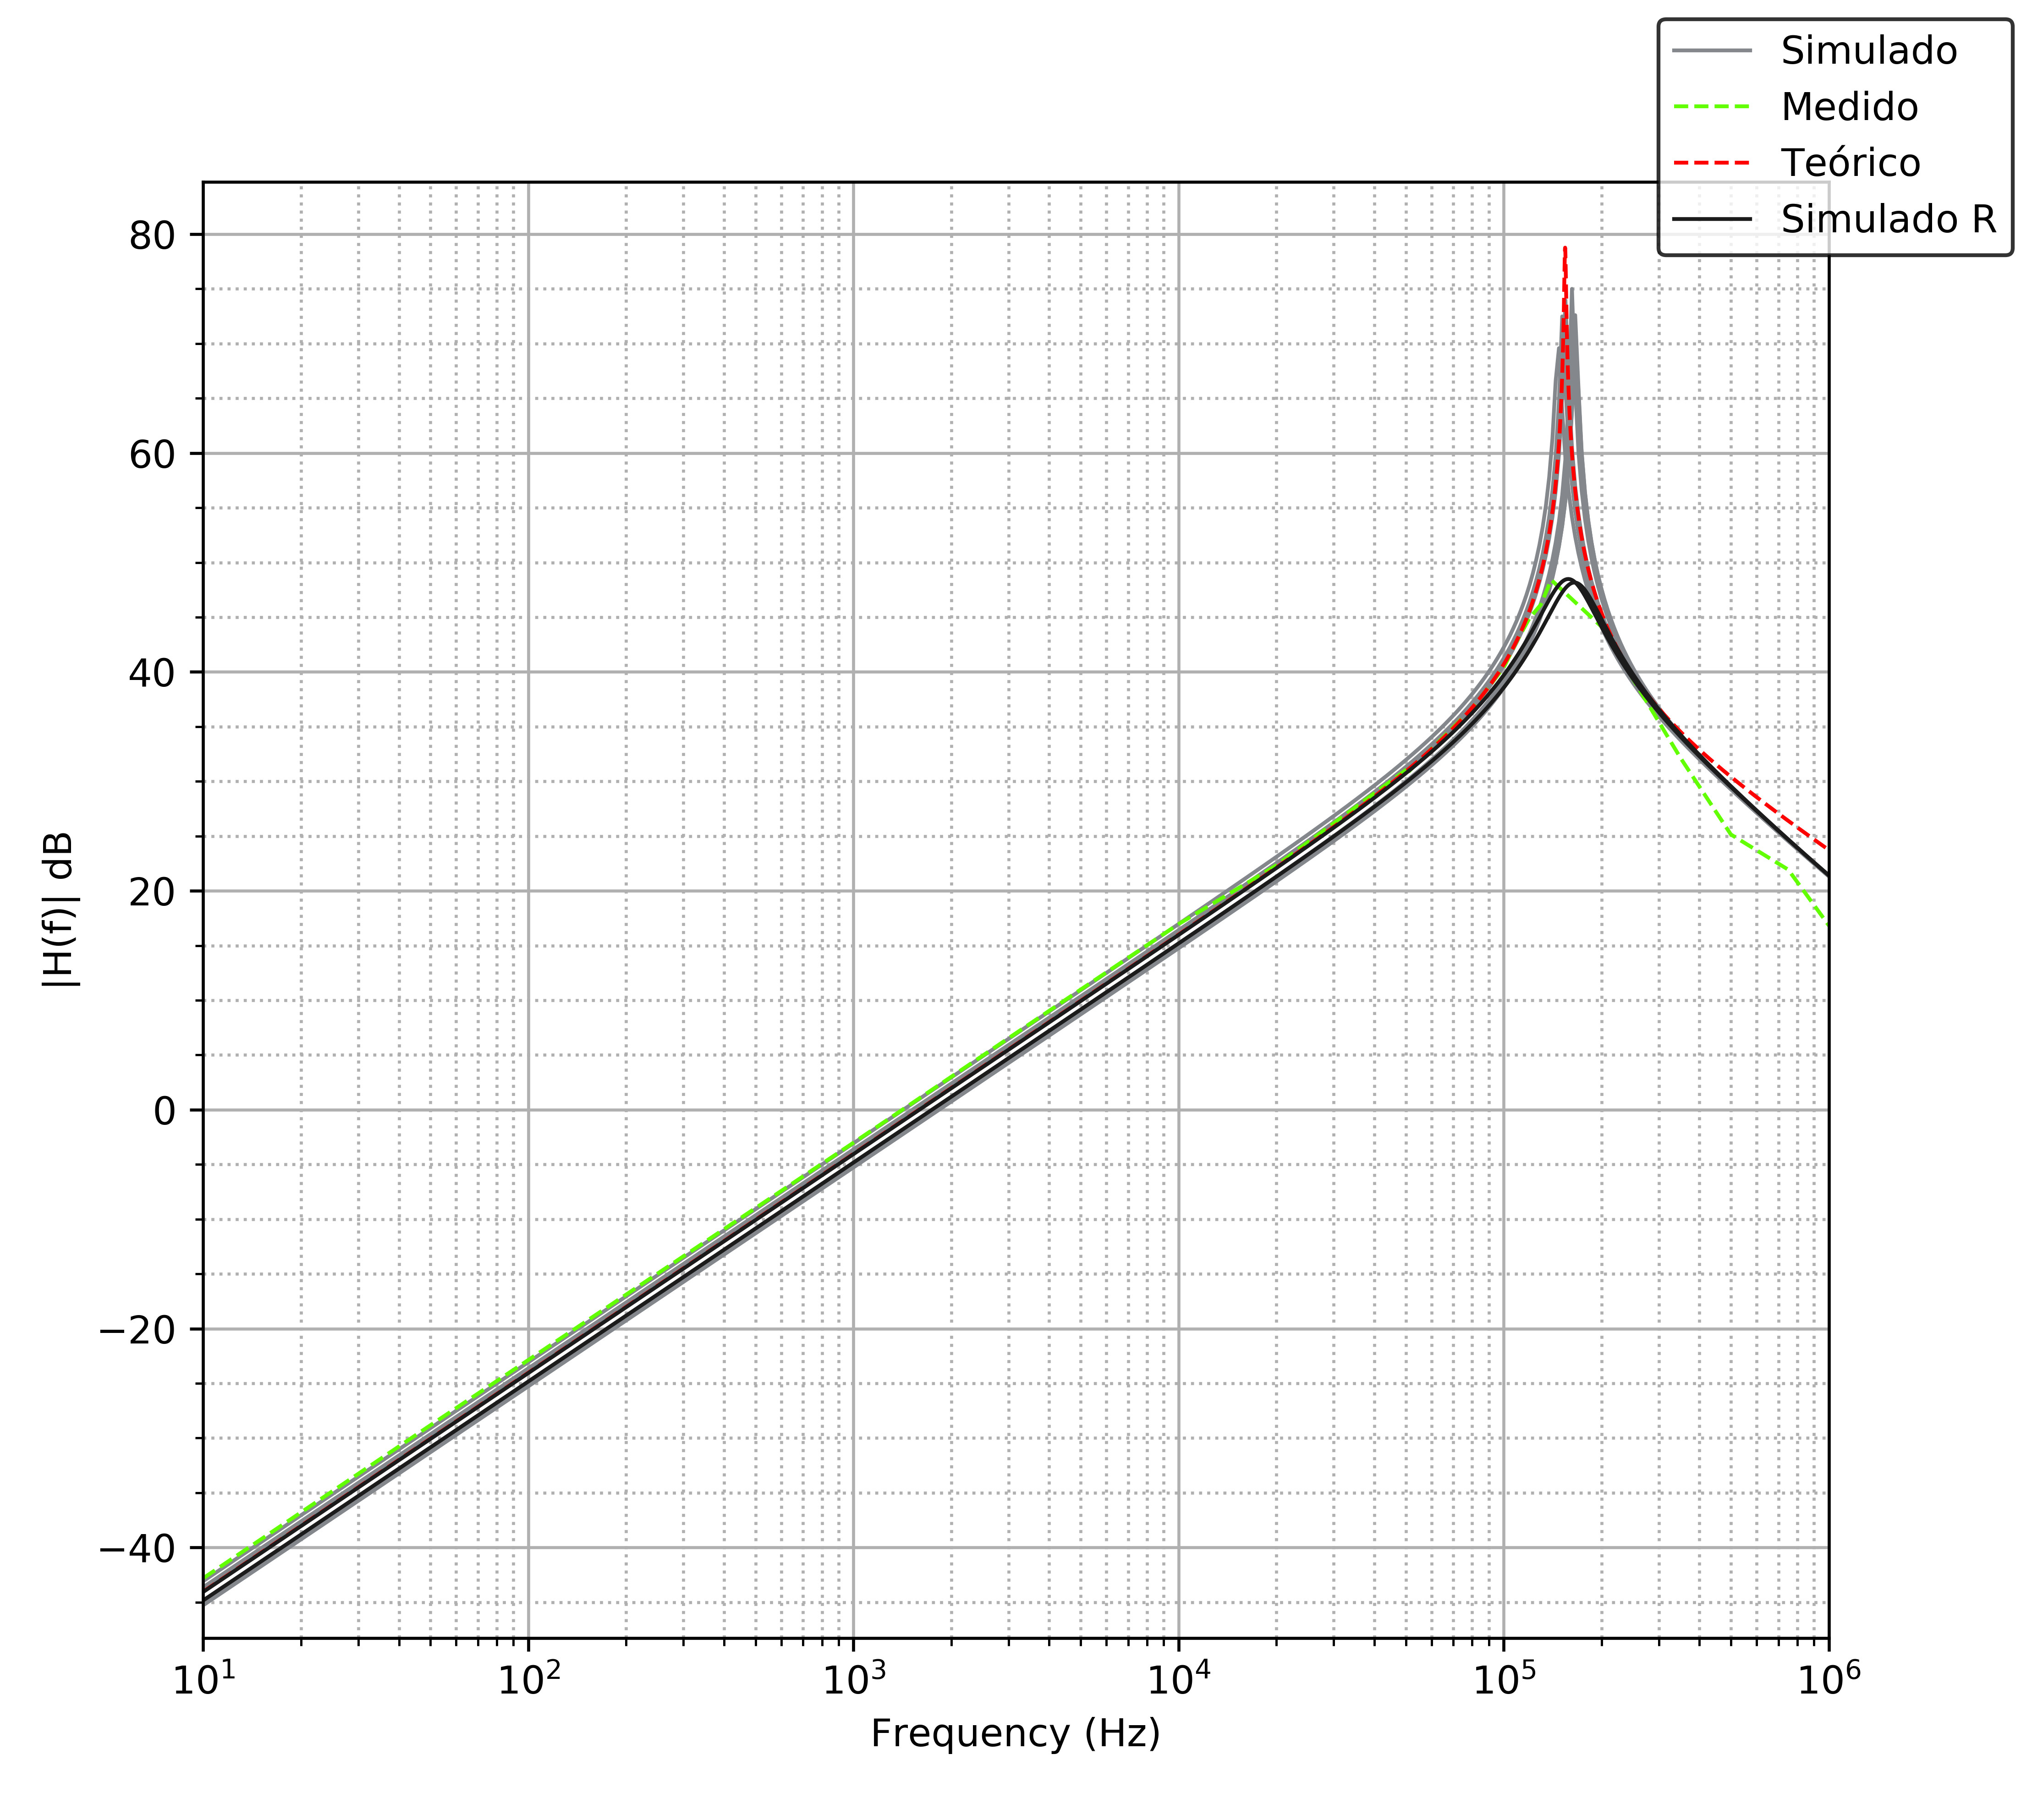
\includegraphics[scale=0.6]{Recursos/Derivador/bode_modulo_correcion.png}
	\caption{Diagrama de bode en m\'odulo de H(f) del derivador}
	\label{fig:derivador_bode_modulo}
\end{figure}

\begin{figure}[H]
	\centering
	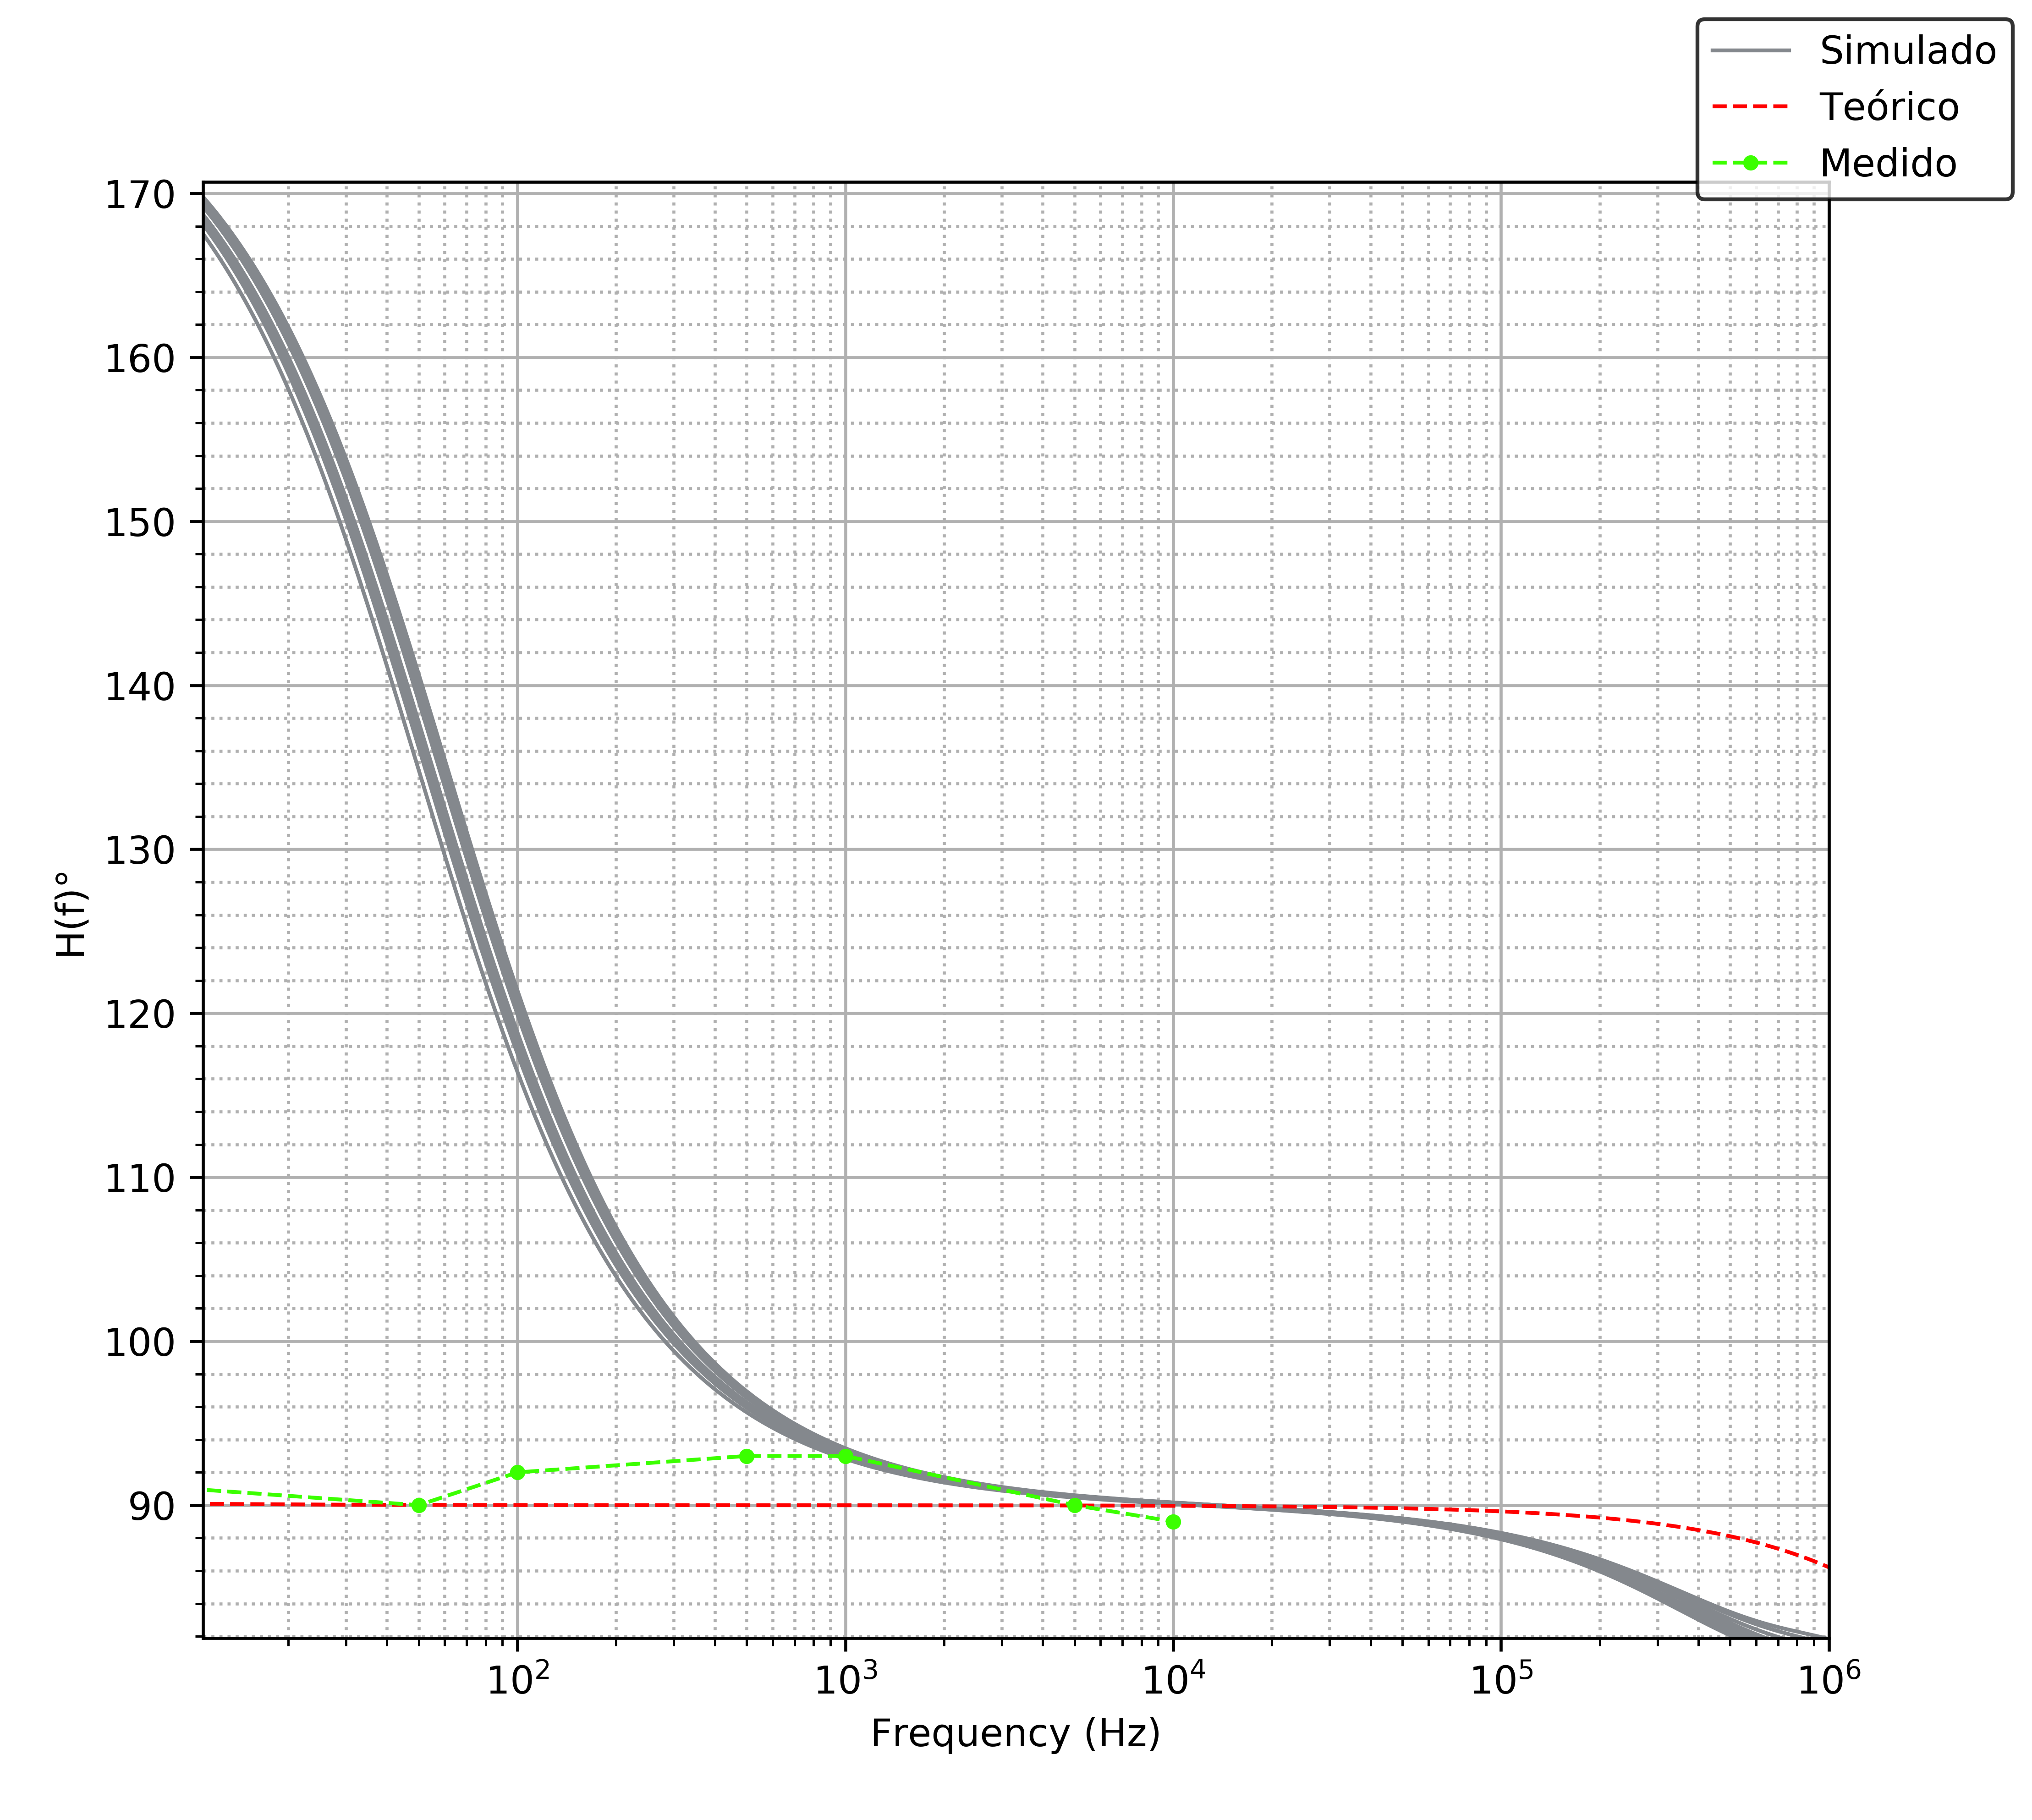
\includegraphics[scale=0.6]{Recursos/Derivador/bode_fase.png}
	\caption{Diagrama de bode en fase de H(f) del derivador}
	\label{fig:derivador_bode_fase}
\end{figure}

\paragraph*{Impedancia de entrada} De los gr\'aficos obtenidos para la medici\'on, simulaci\'on y an\'alisis de la impedancia
de entrada del circuito, se pueden analizar los mismos efectos que para el caso de la respuesta en frecuencia. Esto \'ultimo quiere decir que para frecuencias
menores que $f < 100kHz$ hay poco error entre los resultados obtenidos, mientras que para las dem\'as frecuencias hay desviaciones m\'as apreciables, y se atribuye
al igual que antes al hecho de que para dichas frecuencias la impedancia de entrada produce una gran atenuaci\'on y la ganancia produce saturaci\'on de la salida
con poca tensi\'on, con lo cual no hay forma de obtener para alguna se\~nal de entrada, una salida apreciable, ya que si la tensi\'on pico a pico fuera peque\~na para que no sature,
luego la atenuaci\'on en la entrada por el divisor de tensi\'on entre carga y generador provocar\'ia que no llegue una se\~nal de magnitudes apreciables. Adem\'as llegado el caso
donde estos aspectos no afecten, se ver\'ia que para tales frecuencias el slew rate limitar\'ia la pendiente de crecimiento.

\begin{figure}[H]
	\centering
	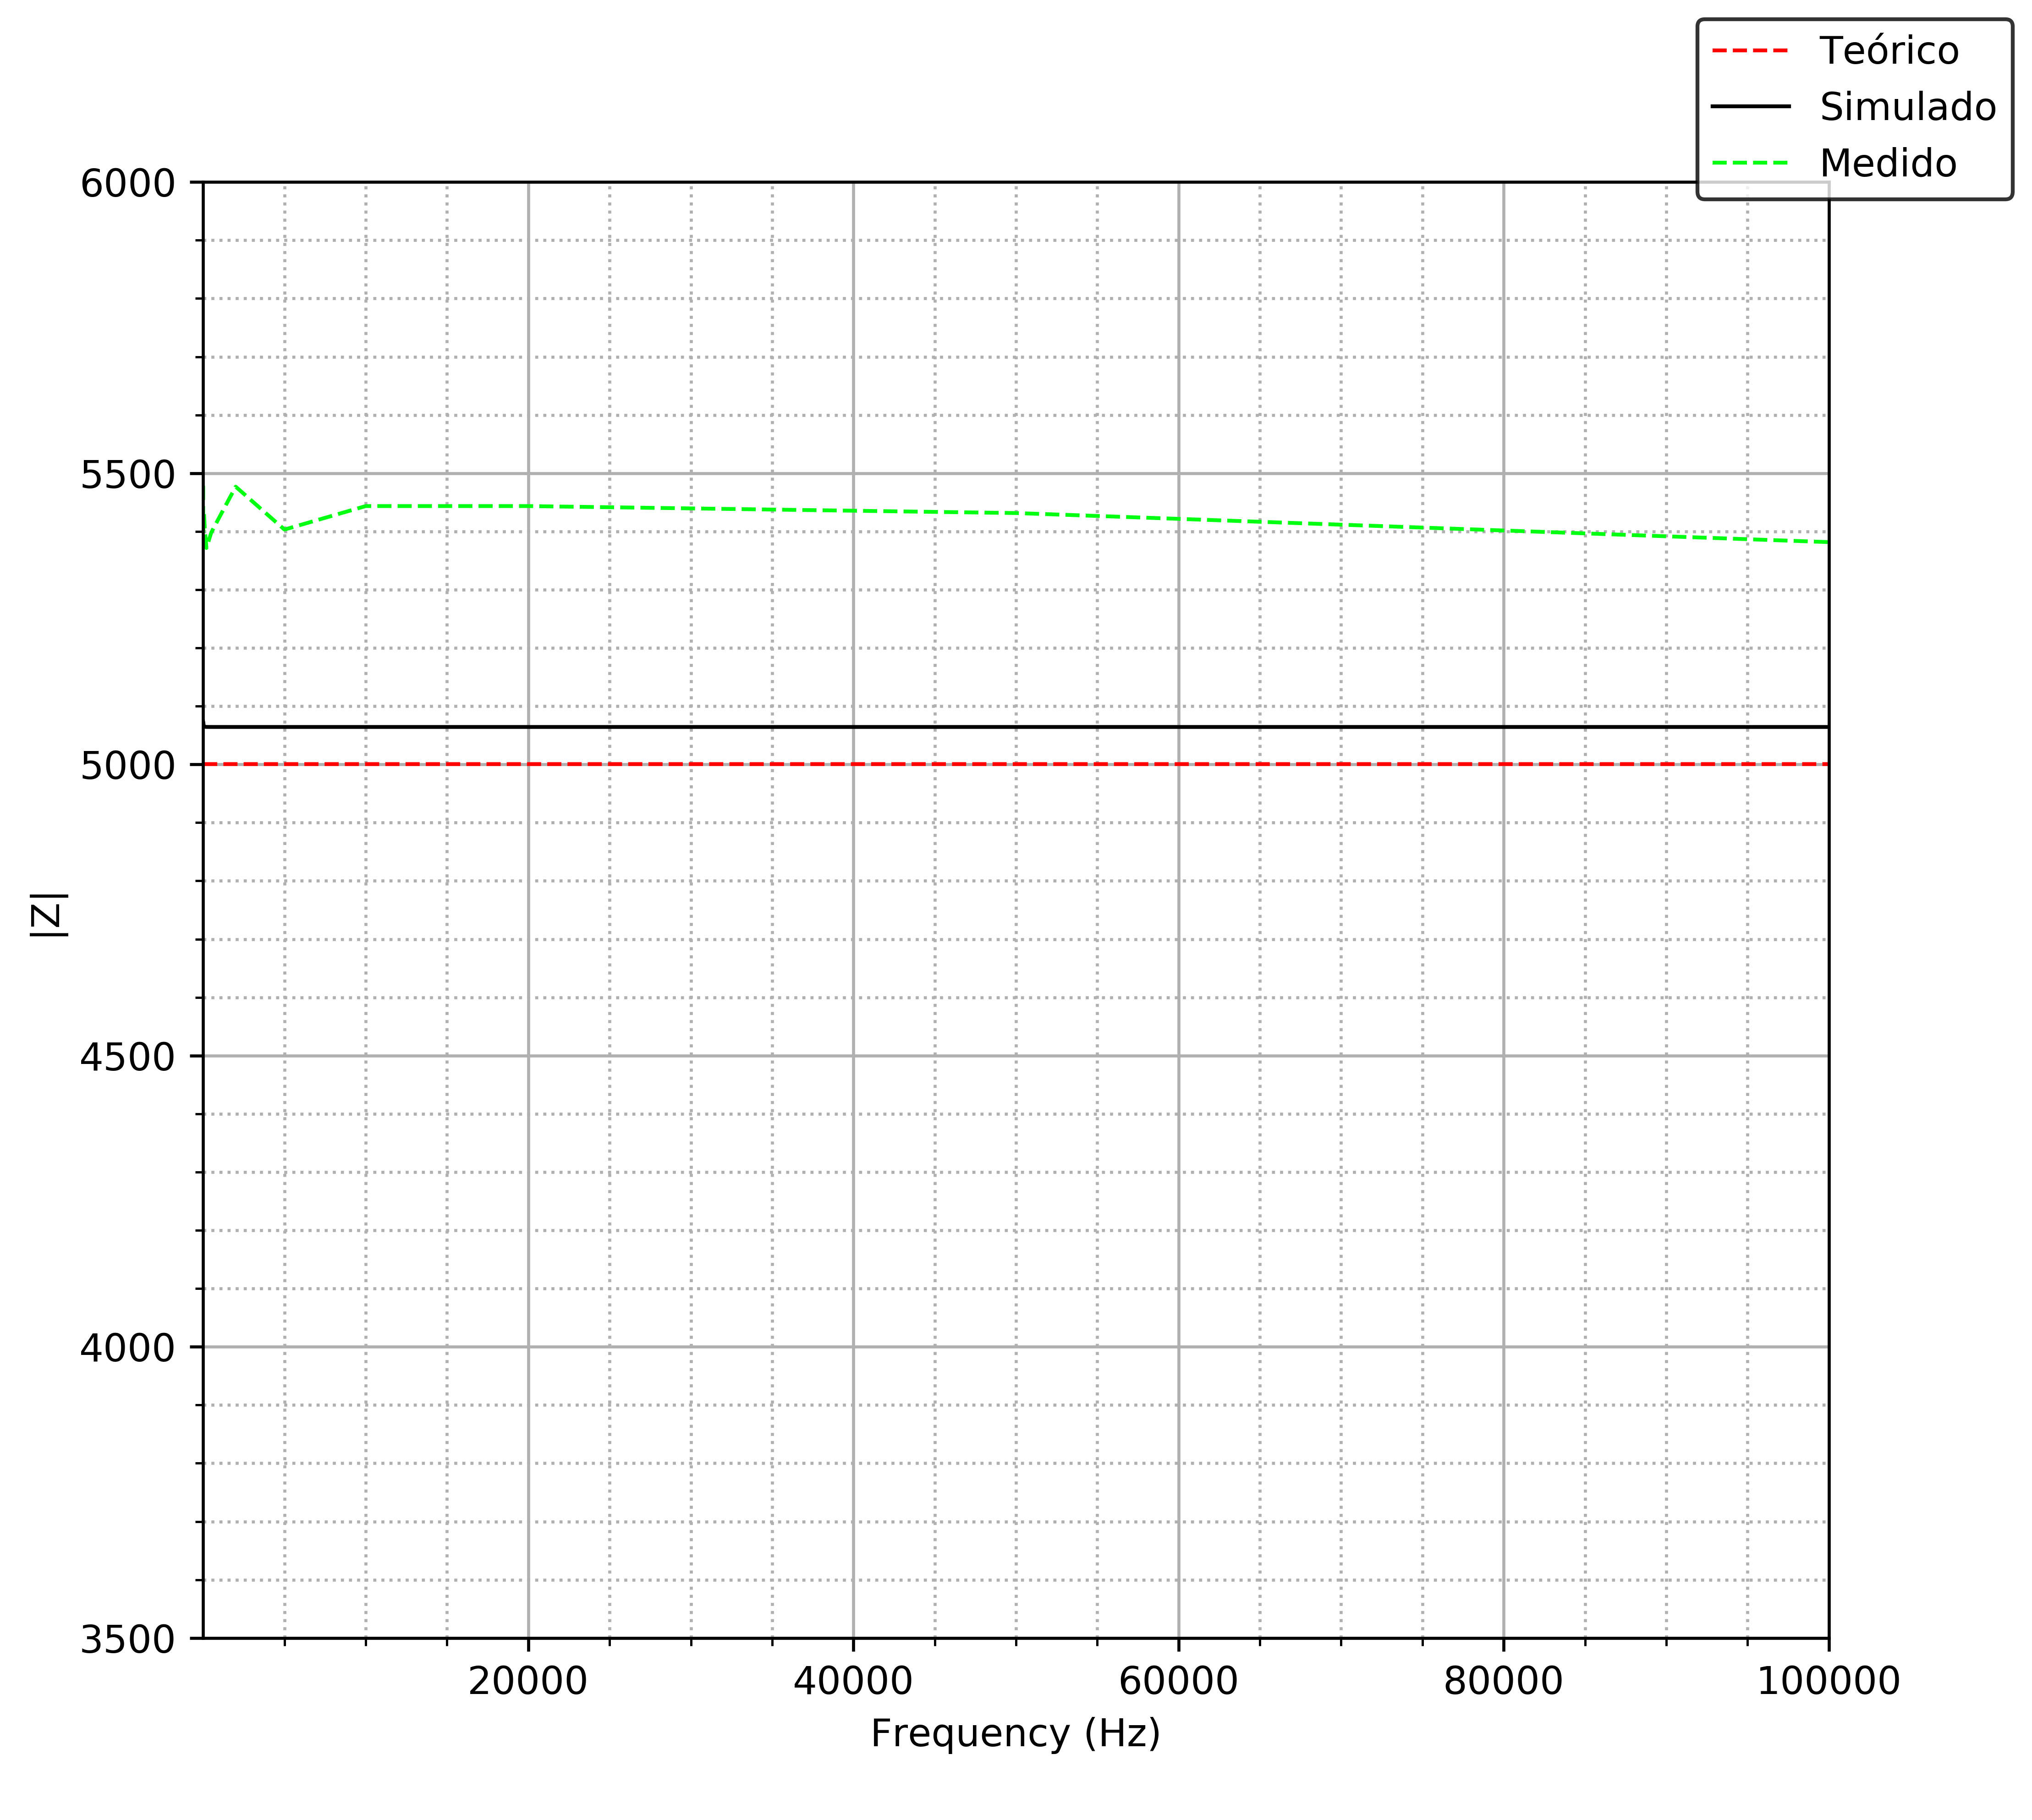
\includegraphics[scale=0.7]{Recursos/Derivador/impedancia_modulo.png}
	\caption{Impedancia de entrada en m\'odulo, graficada con escalas logar\'itmicas}
	\label{fig:derivador_impedancia_modulo}
\end{figure}

\begin{figure}[H]
	\centering
	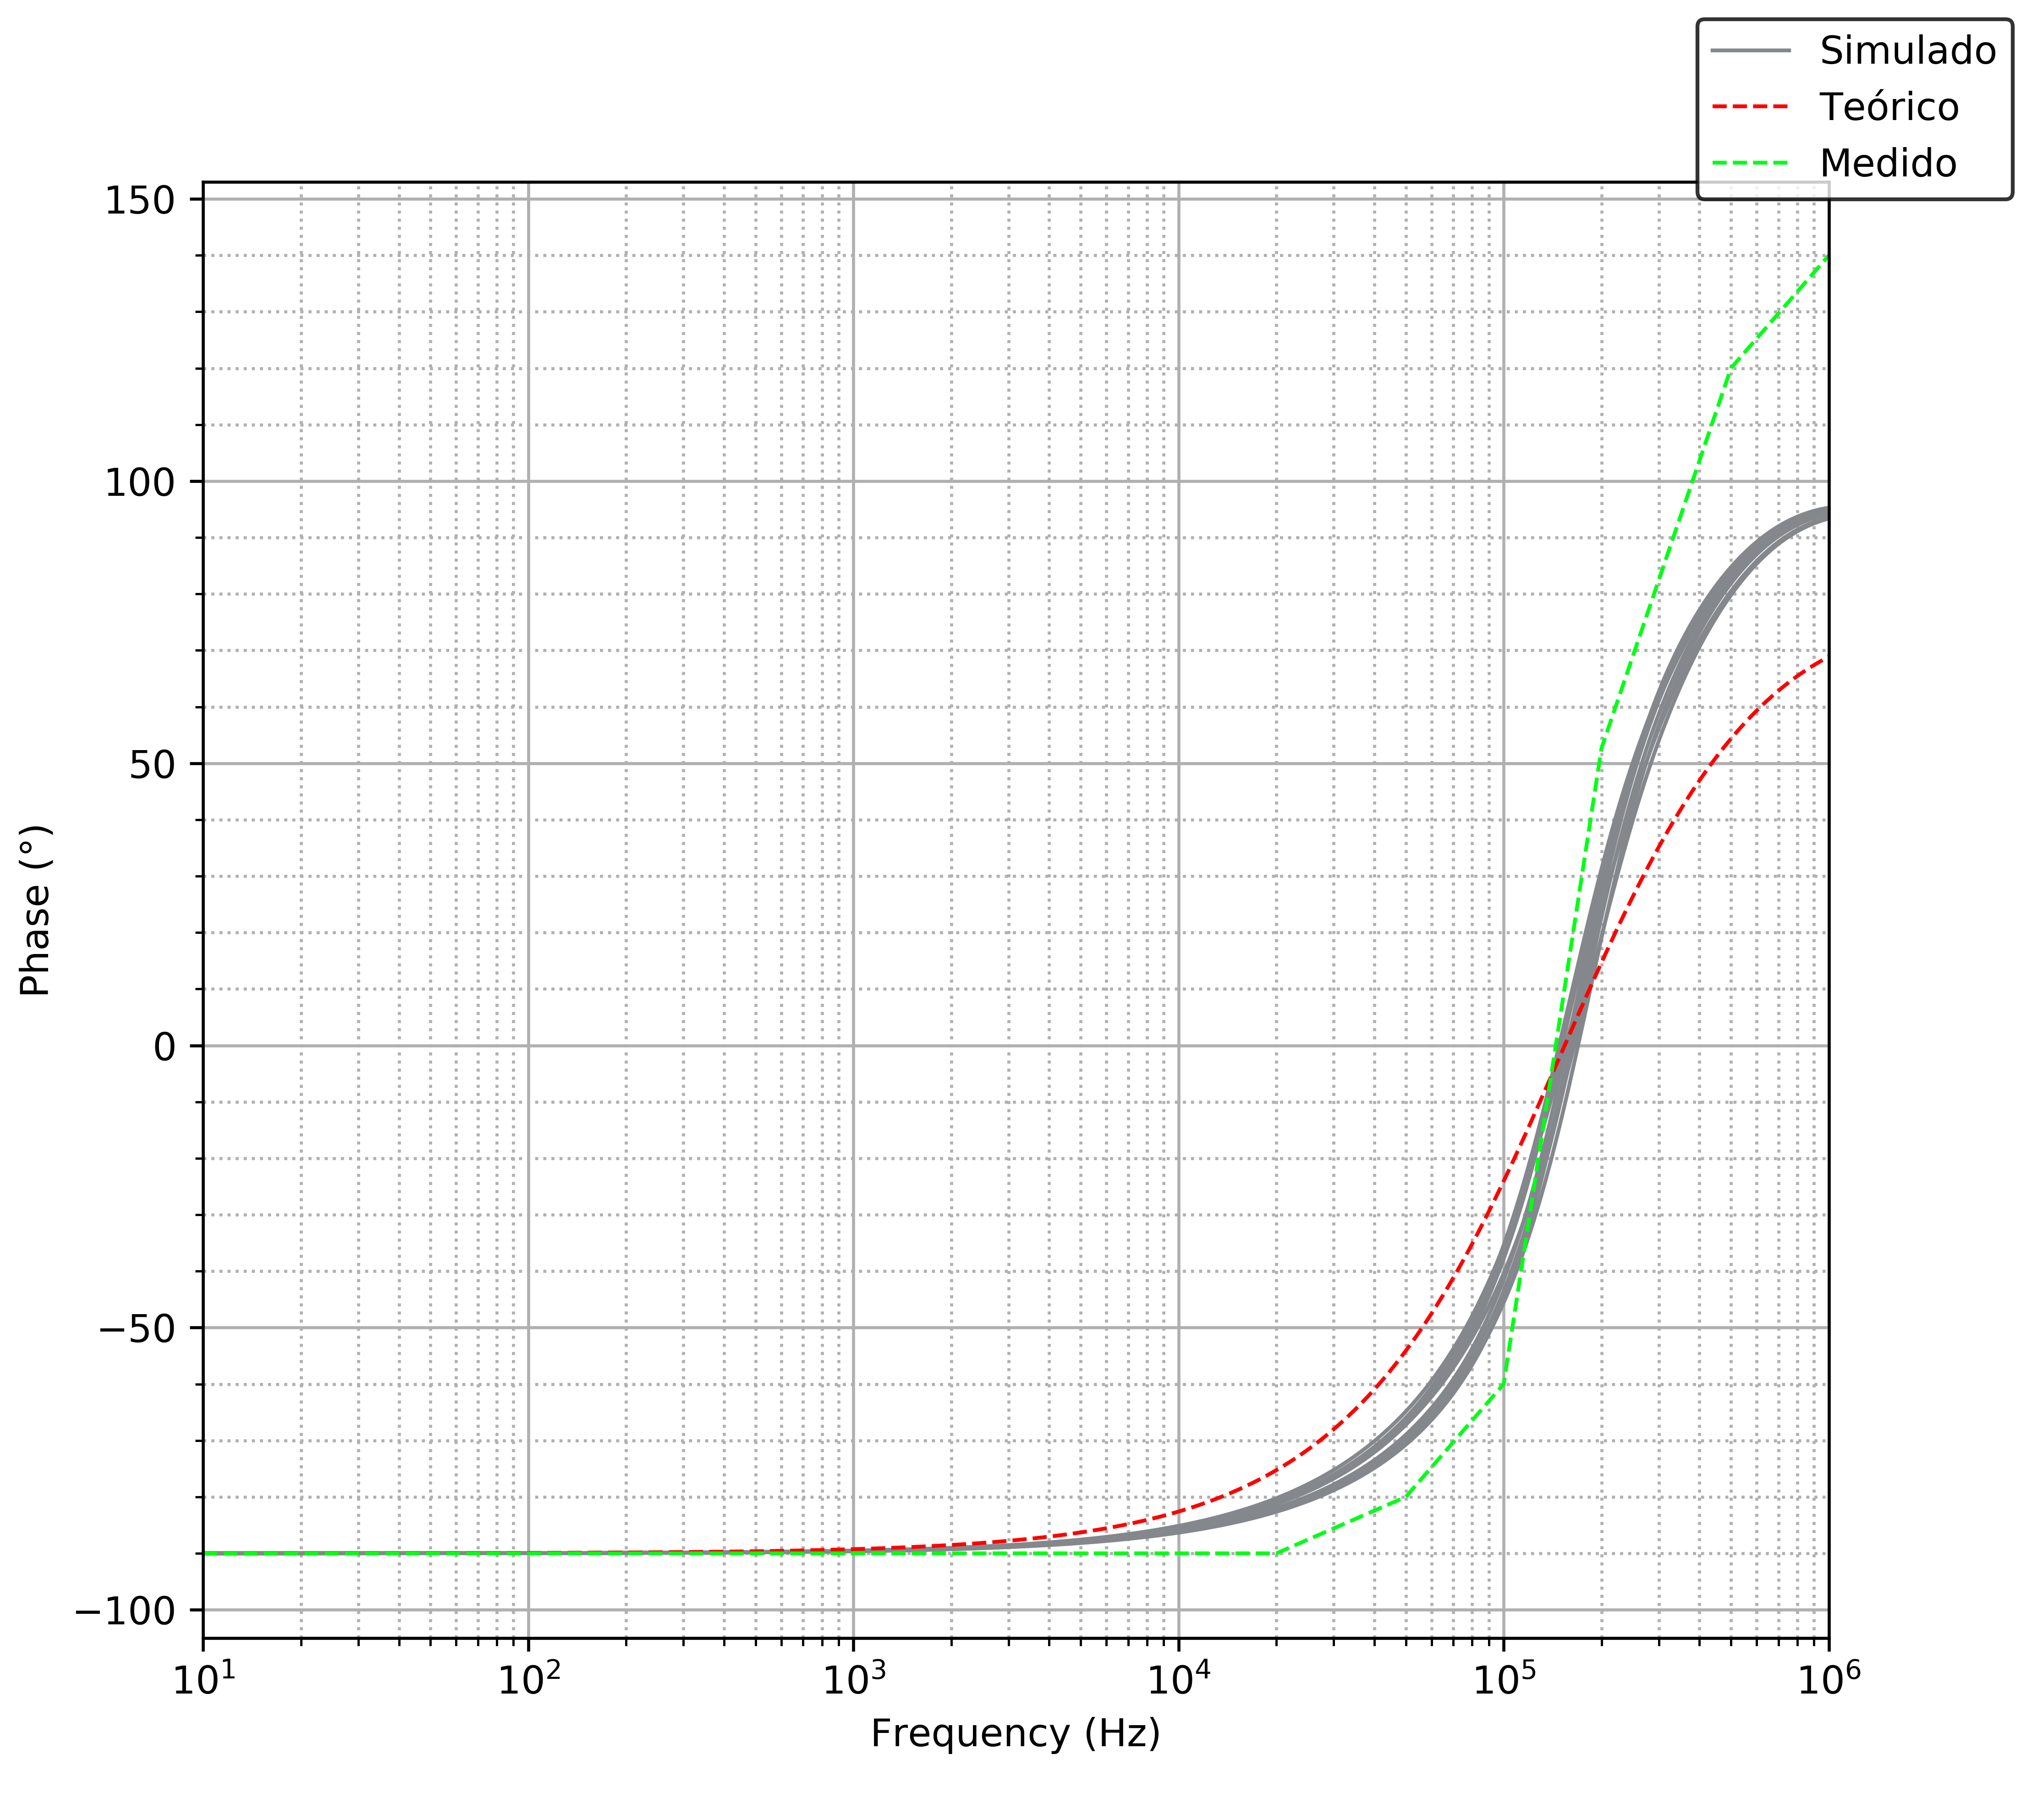
\includegraphics[scale=0.7]{Recursos/Derivador/impedancia_fase.png}
	\caption{Impedancia de entrada en fase, graficada con escalas logar\'itmicas}
	\label{fig:derivador_impedancia_fase}
\end{figure}

\paragraph*{Respuesta a señales no senoidales} en la figura \ref{fig:derivador_respuestas} se pueden observar las respuestas
al derivador sin compensar para cuatro casos diferentes, una triangular con simetr\'ia del $80\%$ y una frecuencia de $10kHz$,
una triangular con simetr\'ia de $50\%$ y frecuencia de $1kHz$, una cuadrada de frecuencia $1kHz$ con duty del $50\%$ y finalmente una cuadrada
de frecuencia $10kHz$ y duty del $50\%$.

De estos resultados y otros que pueden observarse cambiando la frecuencia y amplitud de los est\'imulos mencionados, puede observarse que al estar subamortiguado,
el sistema tiene una respuesta transitoria que afecta a la transici\'on de los estados de la salida, y si bien puede apreciarse la operaci\'on de derivar sobre la misma,
la oscilaci\'on amortiguada se presenta como un efecto indeseado cuando lo que se busca en el sistema es puramente el proceso de derivar la entrada. Esto implica que desde otro enfoque distinto,
el temporal, se pueden contrastar otras consecuencias del subamortiguamiento del sistema adem\'as de las obtenidas en el dominio de la frecuencia. Tales consecuencias son las que dan pie a la necesidad
de compensar el circuito de alguna forma, como se ver\'a a continuaci\'on.

\begin{figure}[H]
	\centering
	\begin{tabular}{c c}
		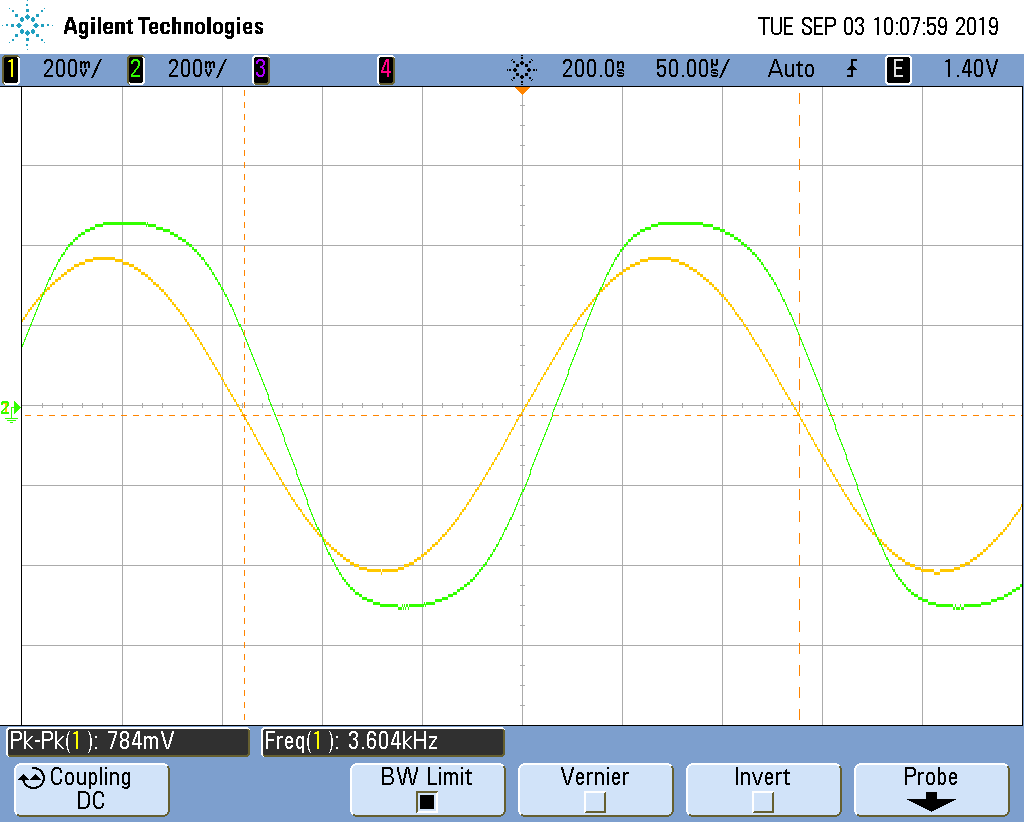
\includegraphics[scale=0.2]{Derivador/Mediciones/Osciloscopio/PCB_Sin_Compensar/scope_11.png} &
		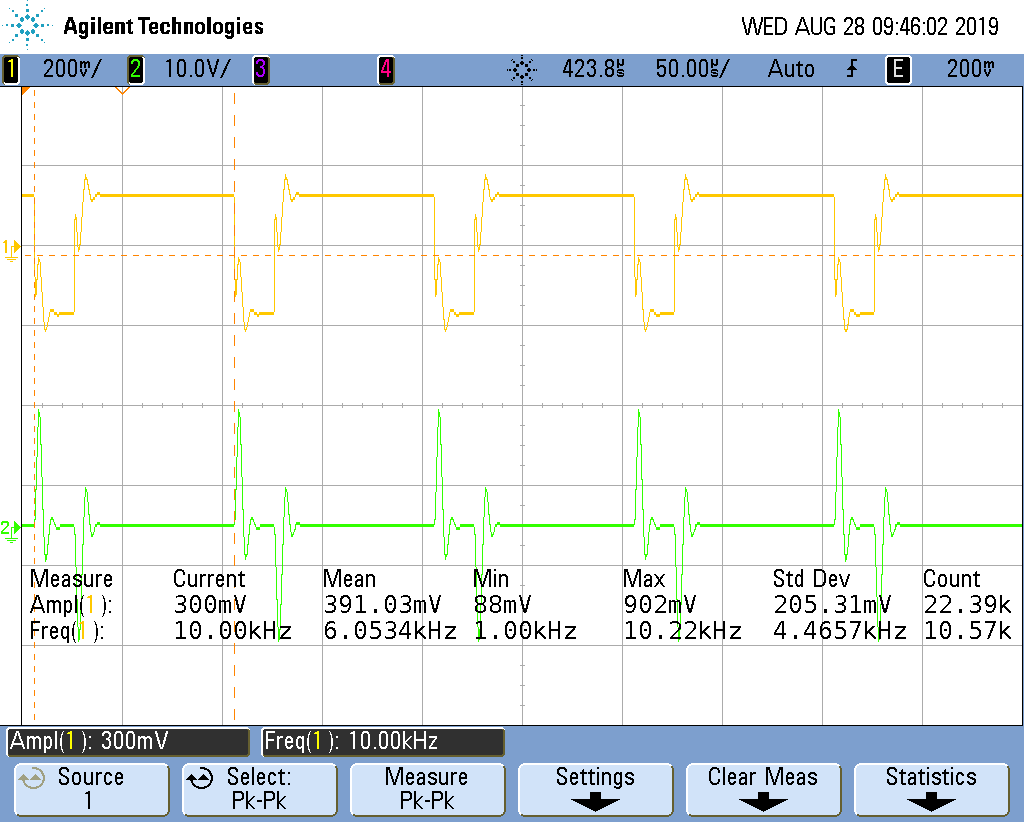
\includegraphics[scale=0.2]{Derivador/Mediciones/Osciloscopio/PCB_Sin_Compensar/scope_3.png} \\
		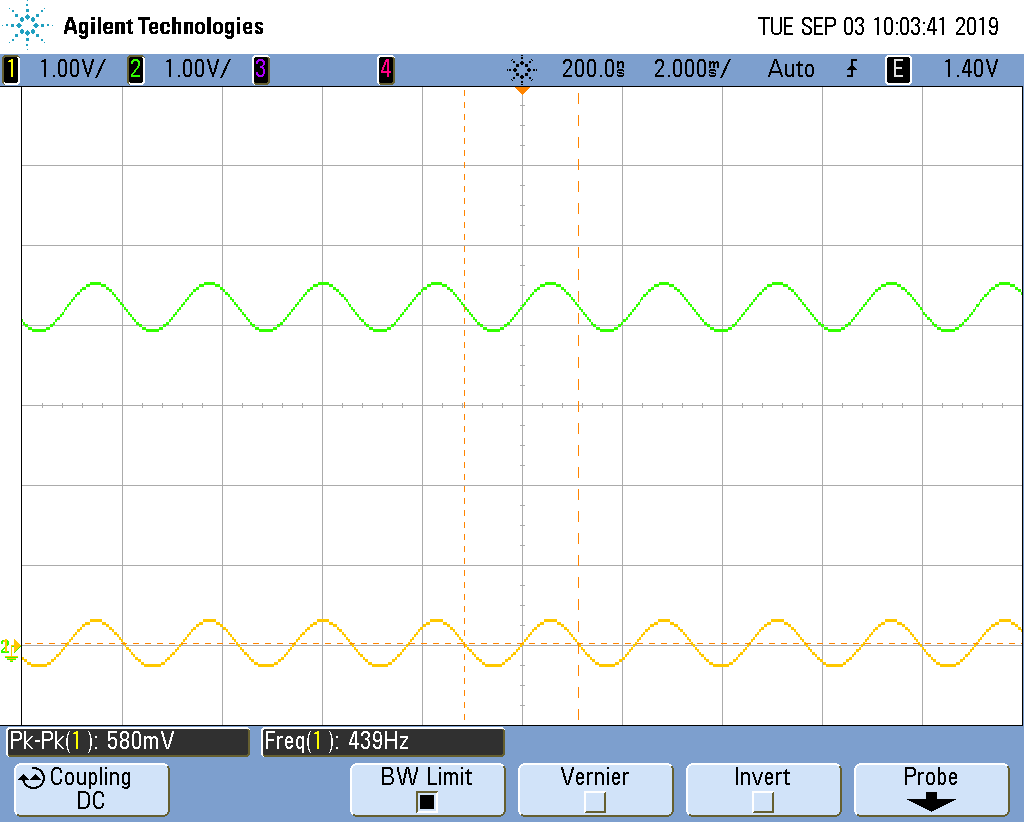
\includegraphics[scale=0.2]{Derivador/Mediciones/Osciloscopio/PCB_Sin_Compensar/scope_5.png} &
		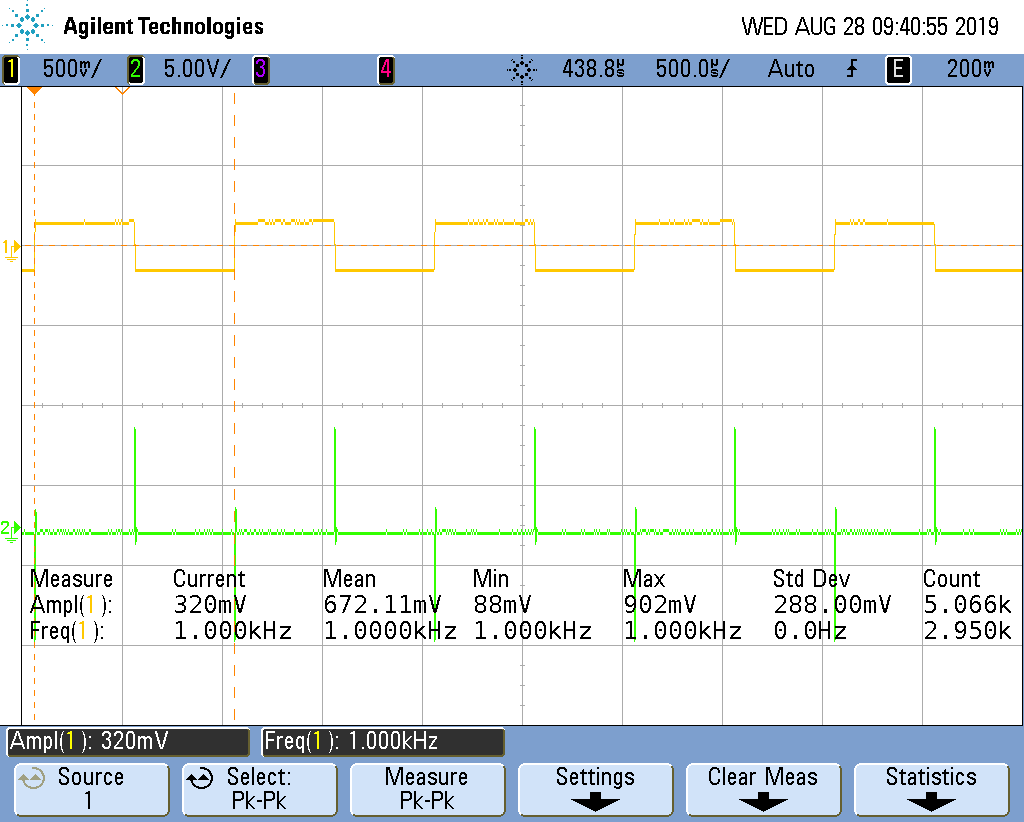
\includegraphics[scale=0.2]{Derivador/Mediciones/Osciloscopio/PCB_Sin_Compensar/scope_7.png}
	\end{tabular}
	\caption{Entrada y salida, señal amarilla y verde respectivamente.}
	\label{fig:derivador_respuestas}
\end{figure}

	\subsection{Circuito derivador compensado}
En la secci\'on anterior se analiz\'o el circuito derivador sin compensaci\'on y se lleg\'o a la conclusi\'on de que, como tal,
si bien ten\'ia un amplio rango de frecuencias en las cuales su comportamiento era la de un derivador, se encontraba en un estado de subamortiguamiento
tanto en funci\'on transferencia como en impedancia de entrada que produci\'a efectos indeseados. Por lo tanto, m\'as all\'a del hecho de que por ser subamortiguado con un bajo
valor de $\xi$ provoca que la transici\'on de fase se haga m\'as abrupta y el margen de funcionamiento como derivador sea mayor, la atenuaci\'on de la impedancia de entrada, saturaci\'on de la salida por ganancia
grande para altas frecuencias y los efectos oscilatorios amortiguados en la transici\'on de la respuesta temporal hacen del circuito anterior un opci\'on poco provechosa.
Por tanto, se propone a continuaci\'on una modificaci\'on al circuito con el fin de compensar tales efectos de la forma m\'as efeciente posible.

\subsubsection{An\'alisis Te\'orico}

\begin{figure}[H]
	\centering
	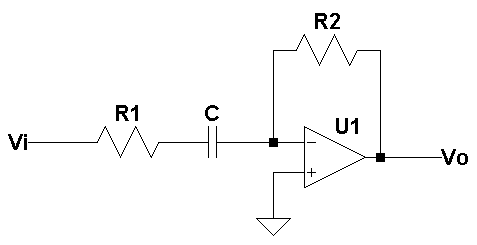
\includegraphics[scale=0.7]{Recursos/Derivador_compensado/Circuito_derivador_compensado.png}
	\caption{Circuito derivador compensado}
	\label{fig:derivador_compensado_circuito}
\end{figure}

En el circuito derivador que se analizar\'a a continuaci\'on se coloca una compensaci\'on 
que consiste en una resistencia en serie en la entrada con el capacitor, esto se debe a que 
se busca compensar los efectos del mismo para altas frecuencias. En altas frecuencias, el 
capacitor tiene una impedancia muy peque\~na con lo cual la ganancia del amplificador 
inversor aumentar\'a y la salida superar\'a la tensi\'on de alimentaci\'on del 
amplificador operacional, produci\'endose as\'i la saturaci\'on del circuito. 
Por otro lado, en cierta parte como la impedancia de entrada depende del capacitor, al 
reducirse tanto a medida que aumenta la frecuencia, disminuye la impedancia de entrada 
y se producen mayores p\'erdidas en la tensi\'on del generador que recibe el circuito.

\paragraph*{Funci\'on transferencia en condiciones ideales} haciendo uso de las condiciones de idealidad que ya se mencionaron para el circuito derivador, a partir de la expresi\'on de la ganancia o transferencia de un amplificador inversor ideal, se llega a que:

\begin{align*}
		H(s) & = \frac{V_o(s)}{V_i(s)} = \frac{-R_2}{R_1 + \frac{1}{s \cdot C}} \\
		& = - \frac{s \cdot C \cdot R_2}{1 + s \cdot C \cdot R_1} \\
\end{align*}

\paragraph*{Funci\'on transferencia con $A_{vol}$ finito} asumiendo que la corriente de entrada del amplificador operacional no es apreciable con respecto a las corrientes de la red L de realimentaci\'on, se plantean las tensiones en las entradas y utilizando la expresi\'on de tensi\'on de salida, se obtiene que:

\begin{equation*}
	v^{-} = V_o \cdot \frac{R_1 + \frac{1}{s \cdot C}}{R_1 + R_2 + \frac{1}{s \cdot C}} + V_i \cdot \frac{R_2}{R_1+ R_2 + \frac{1}{s \cdot C}}
\end{equation*}

\begin{equation*}
	V_o = (v^{+} - v^{-}) \cdot A_{vol} \Rightarrow
	V_o \cdot \left[ 1 + \frac{A_{vol} \cdot (1 + s \cdot C \cdot R_1)}{1 + s \cdot C \cdot (R_1 + R_2)} \right] =
	- V_i \cdot \frac{A_{vol} \cdot (s \cdot C \cdot R_2)}{1 + s \cdot C \cdot (R_1 + R_2)}
\end{equation*}

\begin{equation}
	H(s) = \frac{V_o(s)}{V_i(s)} = - \frac{\frac{s \cdot A_{vol} \cdot C \cdot R_2}{1 + A_{vol}}}{1 + s \cdot \frac{C \cdot (R_2 + R_1 \cdot(1 + A_{vol}))}{1 + A_{vol}}}
	\label{eq:derivador_compensado_finito}
\end{equation}

\paragraph*{Funci\'on transferencia con polo dominante} finalmente si se considera la ecuaci\'on anterior obtenida en \ref{eq:derivador_compensado_finito} y se reemplaza el $A_{vol}$ por la funci\'on que contiene el polo dominante, entonces se llega a que:

\begin{align*}
	H(s) & = \frac{-s \cdot C \cdot R_2 \cdot A_o}{\left( 1 + \frac{s}{\omega_p} \right) \cdot \left( 1 + s \cdot C \cdot (R_1 + 	R_2) \right) + A_o \cdot(1+ s \cdot C \cdot R_1)} \\
	& = - \frac{ \frac{s \cdot c \cdot R_2 \cdot A_o}{A_o + 1} }{1 + s \cdot \frac{1+ \omega_p \cdot \left( A_o \cdot C \cdot R_1 + C \cdot ( R_1 + R_2) \right)}{\omega_p \cdot ( 1 + A_o)} + s^{2} \cdot \frac{C \cdot (R_1 + R_2)}{\omega_p \cdot (1+ A_O)}}
\end{align*}

De esta \'ultima expresi\'on se puede ver del denominador que hay un segundo orden, entonces se procede a obtener sus par\'ametros caracter\'isticos y as\'i determinar su comportamiento.

\begin{equation}
	\omega_o = \sqrt{\frac{\omega_p \cdot ( A_o + 1 ) }{C \cdot ( R_1 + R_2 ) }}
\end{equation}

\begin{equation}
	\xi = \frac{\left[ 1 + \omega_p \cdot C \cdot ( R_1 \cdot (1 + A_o) + R_2) \right] }{2 \cdot \sqrt{\omega_p \cdot C \cdot (A_o + 1) \cdot (R_1 + R_2)}}
	\label{eq:formula_xi}
\end{equation}

Ahora bien, para poder completar el an\'alisis del circuito es necesario determinar el valor de la resistencia $R_1$ la cual no ha sido determinada pues fue agregada a forma de compensaci\'on. Para poder determinar su valor se requieren los siguientes criterios: que no hayan sobrepicos en la funci\'on de transferencia y pueda funcionar hasta la mayor frecuencia posible, adem\'as debe tener un error en la fase menor a 3 grados.

Para poder implementar estas condiciones en el circuito, hay que observar que en la funci\'on transferencia seg\'un sea el caso, primero el denominador debe tener un valor de $\xi \geqslant{1}$ dado que se evita as\'i un sistema subamortiguado cuya respuesta en frecuencia presente un sobrepico. Esta condici\'on se cumple partiendo de la ecuaci\'on \ref{eq:formula_xi}:

\begin{align*}
	& \xi \geqslant{1} \Leftrightarrow \\
	& 1 + \omega_p \cdot C \cdot (R_1 \cdot (A_o + 1) + R_2) \geqslant 2 \cdot \sqrt{\omega_p \cdot C \cdot (A_o + 1) \cdot (R_1 + R_2)} \Leftrightarrow \\
	& R_1^{2} \cdot \alpha + R_1 \cdot \beta + \gamma \geqslant 0
\end{align*}

\begin{align*}
	& \alpha = \omega_p^{2} \cdot C^{2} \cdot (A_o+1)^{2} \\
	& \beta = 2 \cdot \omega_p \cdot C \cdot ( A_o + 1 ) \cdot (R_2 \cdot \omega_p \cdot C - 1) \\
	& \gamma = (1 + \omega_p^{2} \cdot R_2^{2} \cdot C^{2} + \omega_p \cdot C \cdot R_2 \cdot(- 2 - 4 \cdot A_o)
\end{align*}

Resolviendo la cuadr\'atica y encontrando sus ra\'ices, se puede ver que el rango de resistencia con sentido f\'isico para los cuales se logra que el sistema se comporte sobreamortiguado o cr\'iticamente amortiguado, son aquellos donde $R_1 \geqslant 103,48 \Omega$. Por otro lado, para conseguir que el circuito derivador opere hasta la mayor frecuencia posible, habiendo descartado el casos subamortiguado para evitar los sobrepicos en la respuesta en frecuencia, se desea que en el caso \'optimo se encuentre en un amortiguamiento cr\'itico. Esto se debe a que de esta forma en la mayor frecuencia de corte posible se produce la ca\'ida a 40dB/dec, mientras que en un escenario sobreamortiguado el polo se separar\'ia en dos frecuencias de corte reduciendo el ancho de banda disponible.

Con el fin de cumplir con estas condiciones y obtener como resultado el circuito con mejor rendimiento en t\'erminos del ancho de banda donde opera, se coloca un preset en vez de una resistencia fija para poder calibrar el sistema en un valor de aproximadamente $R = 103,487 \Omega$. 

Este proceso de calibraci\'on consiste en utilizar el generador de funciones para excitar al circuito con un escal\'on. Por ser una entrada $V_i(s) = \frac{K}{s}$ con K un valor de amplitud dado, y tener un sistema derivador, la salida debiera de ser una delta de dirac que se ver\'a acotada por la saturaci\'on del amplificador operacional. No obstante, en la transici\'on de la respuesta del circuito se ver\'a la respuesta natural del mismo donde se podr\'a analizar si est\'a en cualquiera de los casos subamortiguado, sobreamortiguado o cr\'iticamente amortiguado, con lo cual se debe mover el preset hasta entrar en la zona sobreamortiguada y luego reducir su valor ligeramente hasta observar que en la salida se tiene el decrecimiento exponencial de menor constante de tiempo sin producir subamortiguamiento.

\begin{figure}[H]
	\centering
	\begin{tabular}{c c}
		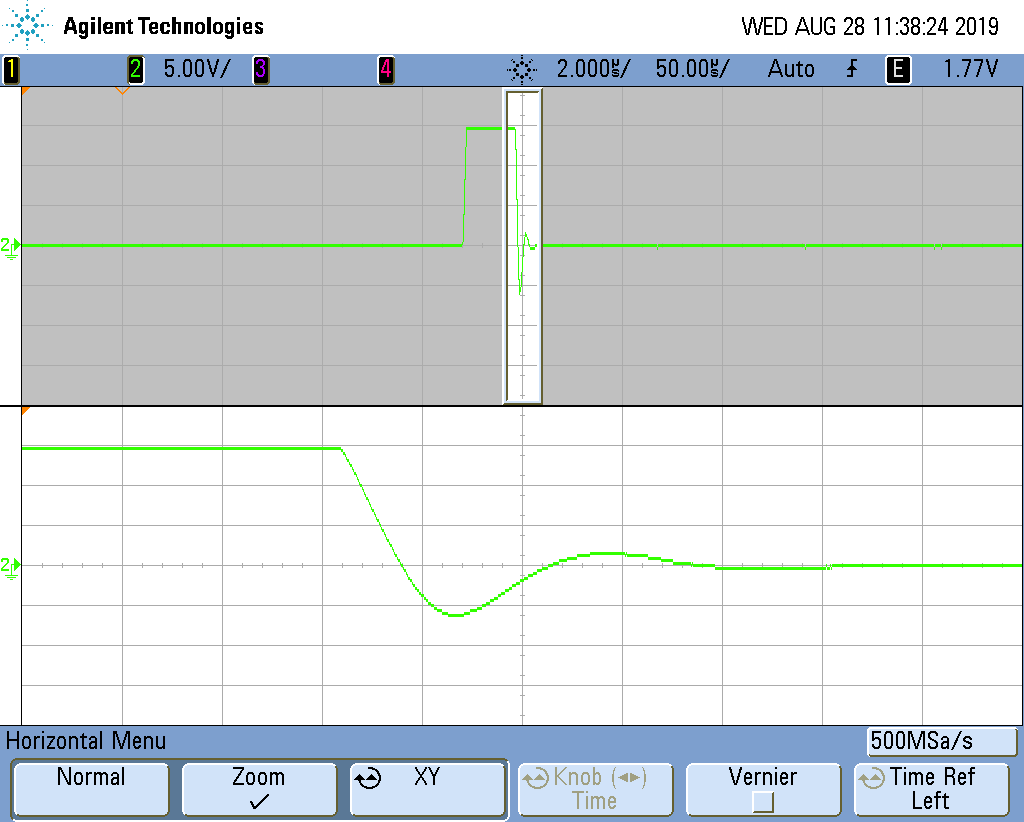
\includegraphics[scale=0.2]{Derivador/Mediciones/Osciloscopio/PCB_Compensado/Calibracion/scope_19.png} &
		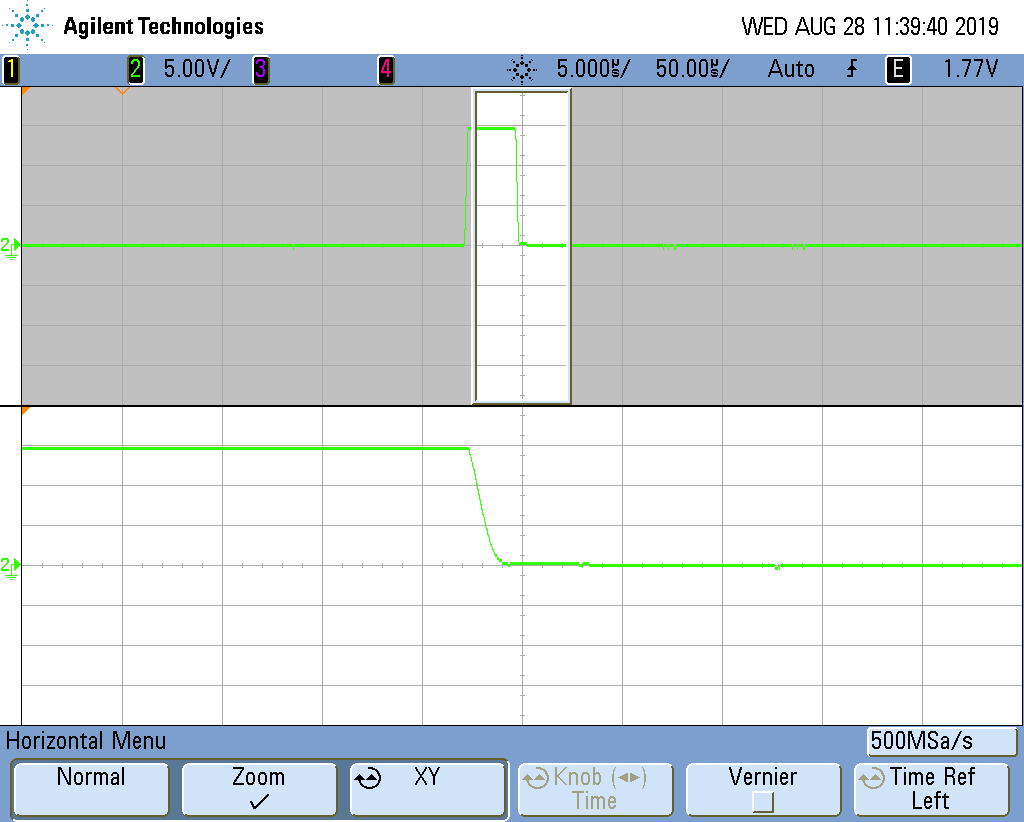
\includegraphics[scale=0.2]{Derivador/Mediciones/Osciloscopio/PCB_Compensado/Calibracion/scope_21.png}
	\end{tabular}
	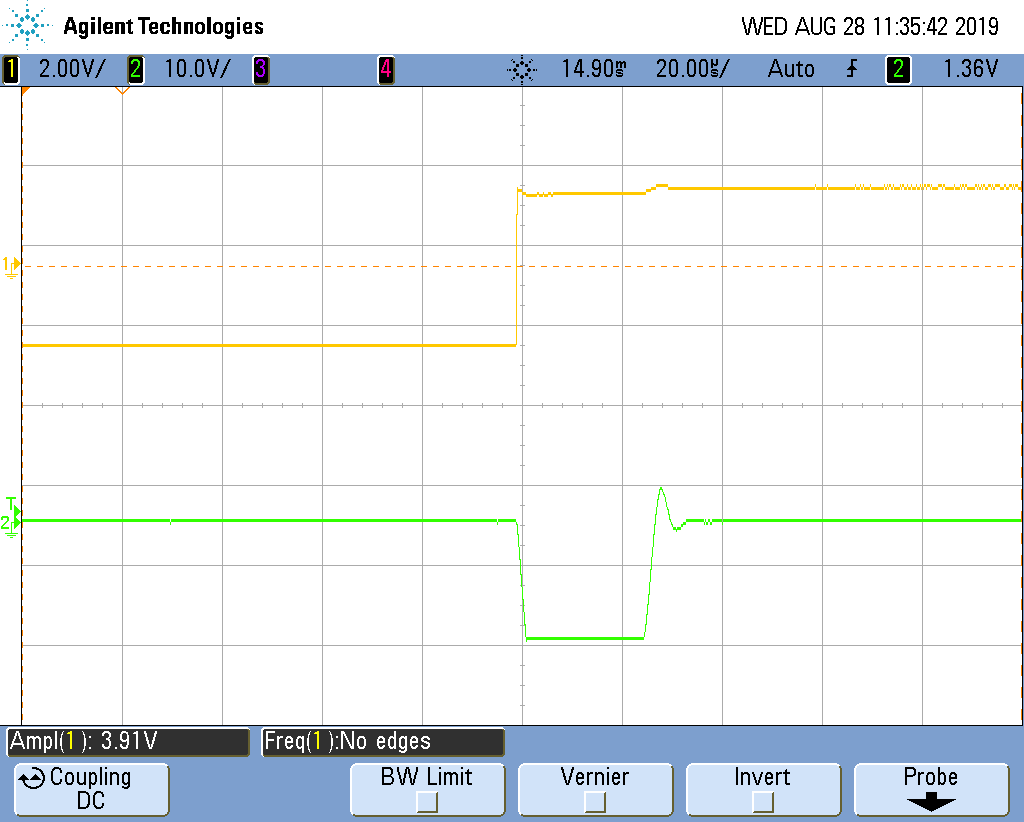
\includegraphics[scale=0.2]{Derivador/Mediciones/Osciloscopio/PCB_Compensado/Calibracion/scope_15.png} 
	\caption{Calibraci\'on del sistema desde el estado subamortiguado al cr\'iticamente amortiguado}
	\label{fig:calibracion_derivador}
\end{figure}

La figura \ref{fig:calibracion_derivador} muestra la realizaci\'on pr\'actica de la calibraci\'on propuesta, donde para la se\~nal amarilla de entrada, sea un escal\'on,
se produce una salida que se encuentra saturada y corresponde a un delta de dirac que idealmente debiera de tender a infinito. Utilizando la base de tiempo retardada del osciloscopio, se hace
zoom sobre la respuesta transitoria del sistema y se calibra tal cual fue descripto previamente hasta llegar al estado cr\'iticamente amortiguado.

\paragraph*{Impedancia de entrada con $A_{vol}$ finito} agregar una nueva resistencia en la entrada del circuito modifica la impedancia de entrada, de forma tal que el an\'alisis se puede aplicar de igual forma que para cuando no estaba, sumandole al resultado obtenido para el derivador sin compensar la resistencia adicional. Realizando algunos pasos algebraicos, se obtiene que:

\begin{figure}[H]
	\centering
	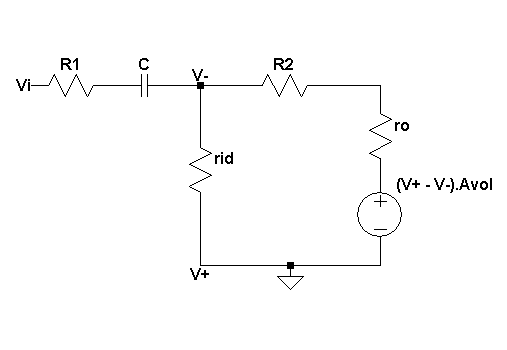
\includegraphics[scale=0.75]{Recursos/Derivador_compensado/Compensado_modelo_impedancia.png}
	\caption{Modelo equivalente del circuito incluyendo compensaci\'on}
	\label{fig:derivador_compensado_modelo}
\end{figure}

\begin{equation}
	Z_{in}(s) = \frac{1 + s \cdot C  \cdot R_1}{s \cdot C} \cdot \frac{1 + s \cdot \frac{R_1 \cdot C \cdot \left[ 2 \cdot (R_2 + Z_o) + r_{id} \cdot(1 + A_{vol}) \right]}{R_2 + Z_o + r_{id} \cdot (1 + A_{vol})}}{1 + s \cdot \frac{R_1 \cdot C \cdot \left[ (R_2 + Z_o) \cdot 2 + r_{id} \cdot ( 1 + A_{vol}) \right] - C \cdot r_{id} \cdot ( R_2 + Z_o)}{R_2 + Z_o + r_{id} \cdot(1+A_{vol})}}
\end{equation}


\paragraph*{Impedancia de entrada con polo dominante} de igual forma que para el caso anterior, se utilizan los c\'alculos realizados previamente para el circuito derivador sin compensar y luego agrega sumando la resistencia adicional en la entrada del circuito, obteniendo luego de algunos pasos algebraicos la impedancia de entrada para el caso donde se considera el polo dominante:

\begin{align*}
	Z_{in}(s) & = \frac{1}{s \cdot C} \cdot \frac{1 + s \cdot \alpha + s^{2} \cdot \beta}{1 + s \cdot \frac{r_{id} + r_{o} + R_2}{\omega_p \cdot \left[ (A_o + 1 ) \cdot r_{id} + r_o + R_2 \right]}} \\
	\alpha & = \frac{r_{id} + R_2 + r_o + \omega_p \cdot C \cdot \left[ r_{id} \cdot ( R_2 + r_o) + R_1 \cdot(r_{id} \cdot ( A_o + 1) + r_o + R_2) \right] }{\omega_p \cdot \left[ r_o + R_2 + r_{id} \cdot (A_o + 1) \right]} \\
	\beta & = \frac{C \cdot \left[ r{id} \cdot ( R_2 + r_o ) + R_1 \cdot (r_{id} + r_o + R_2)) \right]}{\omega_p \cdot \left[ R_2 + r_o + r_{id} \cdot (A_o + 1) \right] }
\end{align*}

\paragraph*{Expresiones finales} de las expresiones te\'oricas obtenidas para el derivador compensado y luego de realizar el dise\~no para cumplir con los criterios impuestos, considerando que el preset calibrado estar\'a en el entorno de $R_1 = 103,487$, se obtienen las expresiones con valores num\'ericos para realizar las comparaciones te\'oricas. Vale aclarar que en la pr\'actica el preset no tendr\'a dicho valor, sino que la suma entre las resistencia de entrada del generador, las par\'asitas y la del preset dar\'an tal resultado.

\begin{equation}
	H(s) = - \frac{\frac{s}{10000,1}}{1 + s \cdot 2,08 \cdot 10^{-6} + \left( \frac{s}{2\pi \cdot 152,935 kHz}\right)^{2}}
\end{equation}

\begin{equation}
	Z_{in}(s) = \frac{1 + \frac{s}{2\pi \cdot 76,89kHz}}{\frac{s}{2\pi 7,95MHz}} \cdot 
	\frac{1 + s \cdot 2,0806 \cdot 10 ^{-6} + \left( \frac{s}{2\pi \cdot 1,04MHz} \right)^{2}}{1 + s \cdot 2,076 \cdot 10^{-6} - \left( \frac{s}{2 \pi \cdot 155,64kHz} \right)^{2}}
\end{equation}

\subsubsection{Resultados}
En esta secci\'on se realizan las simulaciones, mediciones correspondientes sobre el circuito y se contrastan dicho resultados
con los valores te\'oricos, con el objetivo de determinar la efectividad del circuito propuesto como derivador, y su rango de operaci\'on.

\paragraph*{Respuesta en frecuencia} en el gr\'afico del m\'odulo de la respuesta en frecuencia se pueden observar cuatro conjuntos de curvas
que son f\'acilmente reconocibles como la te\'orica, la medida, y las simuladas. En primer lugar, es necesario prestar atenci\'on a la diferencia entre el resultado
te\'orico y la medici\'on, claramente lo obtenido no cumple con el requisito impuesto donde se buscaba un sistema subamortiguado, ya que se puede observar que la medici\'on 
tiene un ligero sobrepico. No obstante, esta diferencia se debe al hecho de que, si bien el sistema como tal se encuentra cr\'iticamente amortiguado pues fue calibrado analizando
la respuesta transitoria del mismo, la diferencia entre teor\'ia y pr\'actica yace en qu\'e se est\'a midiendo. El an\'alisis te\'orico supone un generador de funciones ideal
sin impedancia en serie, con lo cual la caracterizaci\'on del sistema es directamente estableciendo $H(s) = \frac{V_o}{V_{gen}}$, no obstante en la pr\'actica el generador tiene una resistencia
en serie de $R = 50 \Omega$ y lo que en verdad se est\'a midiendo es $H(s) = \frac{V_o}{V_i}$. Esta diferencia implica que el sistema que fue calibrado como cr\'ticamente amortiguado se compone, conceptualmente,
de una resistencia de compensaci\'on resultante de la agrupaci\'on serie entre el preset y la resistencia del generador.

\begin{figure}[H]
	\centering
	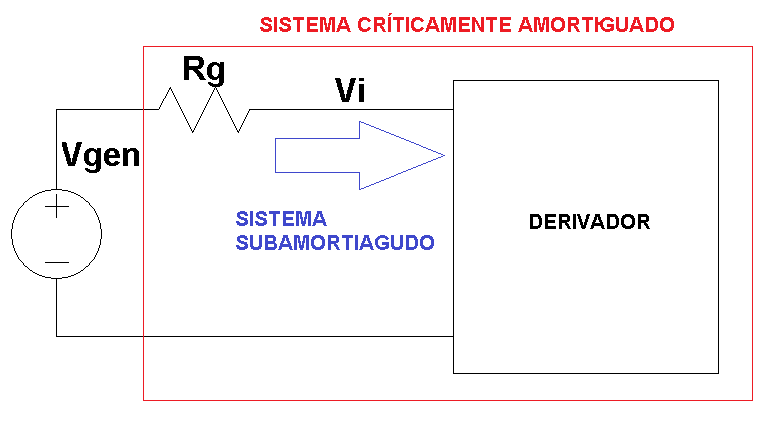
\includegraphics[scale=0.6]{Recursos/Integrador/correccion.png}
	\caption{Diagrama explicativo del error cometido en el dise\~no}
	\label{fig:derivador_correccion}
\end{figure}

Analizando con mayor detalle, los resultados no implican en verdad que haya habido un error, solamente indican
un subamortiguamiento que no caracteriza al sistema que en verdad se debe considerar. Concluyendo, si se caracteriza al sistema a partir de las se\~nales de entrada
y salida que pueden ser medidas, se termina describiendo un sistema subamortiguado que no es el que est\'a siendo puesto a prueba ya que el que verdaderamente es empleado a la hora de derivar se\~nales est\'a cr\'ticamente
amortiguado y su respuesta en frecuencia no puede ser caracterizada, pues ser\'ia necesario medir directamente sobre la $V_{gen}$ del modelo propuesto. Por esto \'ultimo es que se considera que el
m\'etodo de calibraci\'on analizando la respuesta temporal es la mejor forma de observar que el sistema se encuentra cr\'iticamente amortiguado.

\begin{figure}[H]
	\centering
	\includegraphics[scale=0.6]{Recursos/Derivador_compensado/bode_modulo.png}
	\caption{Diagrama de bode en m\'odulo del derivador compensado}
	\label{fig:derivador_compensado_bode_modulo}
\end{figure}

\begin{figure}[H]
	\centering
	\includegraphics[scale=0.6]{Recursos/Derivador_compensado/bode_fase.png}
	\caption{Diagrama de bode en fase del derivador compensado}
	\label{fig:derivador_compensado_bode_fase}
\end{figure}

Finalmente, en principio se puede observar que por el diagrama de bode en fase que se obtuvo de las mediciones,
el circuito puede considerarse derivador hasta una frecuencia aproximadamente de $f_{max} = 15kHz$, donde como se puede
observar a continuaci\'on, si se quisiera que la tensi\'on pico a pico de la se\~nal de entrada permaneciera constante para toda
frecuencia, deberia utilizarse como m\'aximo $V_pp = 2,91 V$ para evitar saturaci\'on de la salida. Estas conclusiones se obtienen de los datos
utilizados para las gr\'aficas realizadas, t\'engase en cuenta que se fueron tomando valores de tensi\'on y frecuencia en los cuales no se produc\'ia
ninguna distorsi\'on o deformaci\'on de la salida, siempre y cuando lo obtenido diera como resultado una medici\'on apreciable.

\begin{table}[H]
	\centering
	\begin{tabular}{c c c c c}%
		$V_{gen} [V]$ & $f_{gen} [Hz]$ & $V_{out} [V]$ & $\phase{V_{out}} [\circ]$ & $\frac{V_o}{V_i} [dB]$ \\ \hline
		\csvreader[head to column names, late after line=\\]{bode_derivador_compensado.csv}{}{\gen & \f & \out & \p & \db}
		\hline
	\end{tabular}
\end{table}

\paragraph*{Impedancia de entrada}

\begin{figure}[H]
	\centering
	\includegraphics[scale=0.7]{Recursos/Derivador_compensado/impedancia_modulo.png}
	\caption{Impedancia de entrada del derivador compensado, en modulo}
	\label{fig:derivador_compensado_impedancia_modulo}
\end{figure}

\begin{figure}[H]
	\centering
	\includegraphics[scale=0.7]{Recursos/Derivador_compensado/impedancia_fase.png}
	\caption{Impedancia de entrada del derivador compensado, en fase}
	\label{fig_derivador_compensado_impedancia_fase}
\end{figure}

\paragraph*{Respuesta a se\~nales no senoidales}

\begin{figure}[H]
	\centering
	\begin{tabular}{c c}
		\includegraphics[scale=0.2]{Derivador/Mediciones/Osciloscopio/PCB_Compensado/EJ_1_TABLA_6.png} &
		\includegraphics[scale=0.2]{Derivador/Mediciones/Osciloscopio/PCB_Compensado/osc_4.png} \\
		\includegraphics[scale=0.2]{Derivador/Mediciones/Osciloscopio/PCB_Compensado/osc_8.png} &
		\includegraphics[scale=0.2]{Derivador/Mediciones/Osciloscopio/PCB_Compensado/scope_23.png} 
	\end{tabular}
	\caption{Medici\'on de respuesta a se\~nales no senoidales}
	\label{fig:respuesta_derivador_compensado}
\end{figure}

	\subsection{Circuito integrador}

\begin{figure}[H]
	\centering
	\includegraphics[scale=0.8]{Recursos/Integrador/Circuito_integrador.png}
	\caption{Circuito integrador sin compensar}
	\label{fig:circuito_integrador}
\end{figure}
\subsubsection{An\'alisis Te\'orico}

\paragraph*{Funci\'on transferencia en condiciones ideales} considerando el sistema LTI, causal y bibo-estable, bajo condiciones de idealidad donde $A_{vol} \rightarrow \infty$, luego como se conoce la expresi\'on para dicho caso del amplificador inversor, se obtiene que:

\begin{equation}
	H(s) = - \frac{\frac{1}{s \cdot C}}{R} = - \frac{1}{s \cdot C \cdot R}
	\Rightarrow
	H(s) = - \frac{1}{\frac{s}{2 \pi \cdot 1,591kHz}}
	\label{eq:integrador_transfer_ideal}
\end{equation}

En este primer acercamiento al comportamiento del circuito, se puede observar en la funci\'on transferencia que se describe un sistema que no es bibo-estable como se asumi\'o en un principio, sino que posee un polo en el origen. Esto \'ultimo tiene sentido porque implica que para entradas acotadas, la respuesta ser\'a la integral de dicha entrada acotada, pudiendo dar un resultado no acotado en el tiempo. Desde otro punto de vista, para frecuencias muy bajas o se\~nales continuas, la impedancia del capacitor en la realimentaci\'on es demasiado grande y provoca una desconexi\'on o un lazo d\'ebil, por lo tanto el amplificador operacional satura puesto que amplifica en t\'erminos de su $A_{vol}$ correspondiente seg\'un sea el caso.

\paragraph*{Funci\'on transferencia con $A_{vol}$ finito} consid\'erese un $A_{vol}$ finito, luego se plantean los valores de potencial el\'ectrico sobre los terminales de las entradas del amplificador operacional y se calcula la salida con la ecuaci\'on correspondiente al modelo del mismo. Entonces, se obtiene:

\begin{equation*}
	v^{-} = V_i \cdot \frac{\frac{1}{s \cdot C}}{\frac{1}{s \cdot C} + R} + V_o \cdot \frac{R}{\frac{1}{s \cdot C} + R}
	\Rightarrow
	v^{-} = \frac{V_i + V_o \cdot s \cdot C \cdot R}{1 + s \cdot C \cdot R}
\end{equation*}

\begin{equation*}
	V_o = (v^{+} - v^{-}) \cdot A_{vol} \Rightarrow
	V_o \cdot \left[ 1 + \frac{A_{vol} \cdot s \cdot R \cdot C}{1 + s \cdot C \cdot R} \right] =
	- V_i \cdot \frac{A_{vol}}{1 + s \cdot C \cdot R}
\end{equation*}

\begin{equation}
	H(s) = \frac{V_o(s)}{V_i(s)} = \frac{-A_{vol}}{1 + s \cdot C \cdot R \cdot (A_{vol} + 1)}
	\Rightarrow
	H(s) = \frac{-100000}{1 + \frac{s}{2 \pi \cdot 0,0159Hz}}
	\label{eq:integrador_transfer_avol_finito}
\end{equation}

Se puede observar que con estas nuevas consideraciones, el sistema dej\'o de ser inestable en t\'erminos de su respuesta, no obstante sigue sucediendo que para frecuencias muy bajas la realimentaci\'on pasa a tener un lazo d\'ebil y satura el amplificador operacional.

\paragraph*{Funci\'on transferencia con polo dominante} ahora se considera que la ganancia del amplificador operacional tiene el polo dominante, con lo cual no se mantiene invariante en frecuencia. Reutilizando la expresi\'on anterior para $A_{vol}$ finito y reemplazando tal t\'ermino por la expresi\'on con el polo dominante se obtiene:

\begin{equation*}
	H(s) = - \frac{A_o \cdot \omega_p}{s + \omega_p + s \cdot C \cdot R \cdot (A_o \cdot \omega_p + s + \omega_p)}
	\Rightarrow
	H(s) = - \frac{A_o}{1 + s \cdot \frac{1 + C \cdot R \cdot \omega_p \cdot ( A_o + 1 )}{\omega_p} + s^{2} \cdot \frac{C \cdot R}{\omega_p}}
\end{equation*}

\begin{equation*}
	H(s) = - \frac{100000}{1 + s \cdot 10,001 + \left( \frac{s}{2 \pi \cdot 488,60Hz} \right)^{2}}
\end{equation*}

En esta nueva expresi\'on de la funci\'on transferencia, el sistema refleja un segundo orden en el denominador del cual se pueden determinar los par\'ametros caracter\'isticos del mismo, obteniendo que $\omega_o = 3069,96 \frac{1}{s}$ y $\xi = 15351,58 \geq 1$. Entonces el sistema se encuentra en un sobreamortiguamiento con frecuencias de corte ubicadas en $f_1 = 15,0017MHz$ y $f_2 = 0,01499Hz$.

\begin{equation}
	H(s) = - \frac{106092,66}{(1 + \frac{s}{2 \pi \cdot 0,014998Hz}) \cdot (1 + \frac{s}{2 \pi \cdot 15,0017MHz})}
	\label{eq:integrador_transfer_polo_dominante}
\end{equation}

En este nuevo resultado la \'unica diferencia con respecto al anterior, es que ahora hay un polo adicional que aparece en una frecuencia muy alejada, no obstante sigue saturando para frecuencias muy bajas por el lazo d\'ebil, es por esto que este circuito no funcionar\'a correctamente con el prop\'osito para el que fue pensado desde un punto de vista ideal, por ende ser\'a necesario realizar alguna compensaci\'on para poder corregirlo.

\paragraph*{Impedancia de entrada con $A_{vol}$ finito} para encontrar la impedancia de entrada considerando el $A_{vol}$ finito, se redibuja el circuito reemplazando al amplificador operacional con su circuito equivalente y se plantea la ley de nodos.
Se llama a la diferencia de potencial $V_d = V^{+} - V^{-}$.

\begin{figure}[H]
	\centering
	\includegraphics[scale=0.7]{Recursos/Integrador/Circuito_integrador_modelo_impedancia.png}
	\caption{Circuito equivalente para c\'alculo de impedancia de entrada}
	\label{fig:integrador_modelo}
\end{figure}

\begin{equation*}
	I_1 = I_2 + I_3 \Rightarrow
	\frac{V_i + V_d}{R_1} = 
	\frac{-V_i}{R_1} + \frac{- V_i - V_i \cdot A_{vol}}{\frac{1}{s \cdot C} + R}
\end{equation*}

\begin{equation*}
	V_d = \frac{- V_i \cdot r_i \cdot ( 1 + s \cdot C \cdot Z_o)}{r_i \cdot(s \cdot C \cdot Z_o + 1) + R_1 \cdot (1 + s \cdot C \cdot Z_o) + s \cdot C \cdot R_1 \cdot r_i \cdot (1 + A_{vol})}
\end{equation*}

\begin{equation*}
	Z_i(s) = \frac{V_i(s)}{I_1(s)} = \frac{V_i(s)}{\frac{V_i(s) + V_d(s)}{R_1}}
	\Rightarrow
	Z_i(s) = (R_1 + r_i) \cdot \frac{1 + s \cdot \frac{C \cdot \left[ Z_o \cdot (R_1 + r_i) + R_1 \cdot r_i \cdot (A_{vol} + 1) \right]}{R_1 + r_i}}{1 + s \cdot C \left[ Z_o + r_i \cdot ( 1 + A_{vol}) \right]}
\end{equation*}

\begin{equation}
	Z_i(s) = (180k \Omega) \cdot \frac{1 + \frac{s}{2 \pi \cdot 0,0163Hz}}{1 + \frac{s}{2 \pi \cdot 0,00045Hz}}
	\label{eq:integrador_impedancia_avol_finito}
\end{equation}

\paragraph*{Impedancia de entrada con polo dominante} reutilizando la expresi\'on anterior para la impedancia de entrada y considerando la variaci\'on del $A_{vol}$ respecto de la frecuencia, se obtiene:

\begin{equation*}
	Z_i(s) = (R_1 + r_i) \cdot \frac{1 + s \cdot \frac{r_i + R_1 + \omega_p \cdot C \cdot \left[ Z_o \cdot ( R_1 + r_i ) + R_1 \cdot r_i \cdot (A_o + 1) \right]}{\omega_p \cdot (R_1 +r_i)} + s^{2} \cdot \frac{C \cdot \left[ Z_o \cdot (R_1 + r_i) + R_1 \cdot r_i \right]}{\omega_p \cdot (R_1 + r_i)}}{1 + s \cdot \frac{1 + \omega_p \cdot C \cdot (Z_o + r_i \cdot ( A_o + 1 ) )}{\omega_p} + s^{2} \cdot \frac{C \cdot(Z_o + r_i)}{\omega_p}}
\end{equation*}

\begin{equation*}
	Z_i(s) = (180k \Omega) \cdot \frac{1 + s \cdot 9,723 + \left( \frac{s}{2 \pi \cdot 493,65Hz} \right)^{2}	}{1 + s \cdot 350,0045 + \left(\frac{s}{2 \pi \cdot 82,58Hz} \right)^{2}}
\end{equation*}

\begin{equation}
	Z_i(s) = 180k \Omega \cdot \frac{(1 + \frac{s}{2 \pi \cdot 25,45Hz}) \cdot (1 + \frac{s}{2 \pi \cdot 9574,06Hz})}{(1 + \frac{s}{2 \pi \cdot 0,1178Hz}) \cdot (1 + \frac{s}{2 \pi \cdot 57,806kHz})}
	\label{eq:integrador_impedancia_polo_dominante}
\end{equation}

\paragraph*{Conclusi\'on del an\'alisis} si se tienen en cuenta las expresiones resultantes para 
la funci\'on transferencia y la impedancia de entrada con la menor idealidad posible, es decir, los
resultados de las Ec. \ref{eq:integrador_transfer_polo_dominante} y
Ec. \ref{eq:integrador_impedancia_polo_dominante}. Asumiendo que el circuito se comportar\'a como
integrador en las regiones de frecuencia para las cuales la fase sea $90^{\circ}$ puesto que podría
aproximarse tal respuesta con la forma de $\frac{-1}{s}$ que en el dominio temporal equivale a la
integral de la funci\'on, luego para frecuencias que cumplan estar en el rango 
$0,14998Hz \leq f \leq 1,5Mhz$ se puede aproximar el comportamiento de la $H(s)$ obtenida a
dicha forma. No obstante, si se consideran bajas frecuencias, la impedancia del capacitor ser\'a 
tan elevada que el lazo de la realimentaci\'on dejar\'a de funcionar como tal, provocando que el
amplificador operacional amplifique en t\'erminos de su $A_{vol}$ con lo cual saturar\'a y dejar\'a de
 funcionar para tales frecuencias. Desde un an\'alisis temporal, y bajo condiciones de idealidad, cualquier componente
 de continua en la entrada provocar\'ia que circule una determinada corriente constante sobre el capacitor provocando
 que su carga acumulada crezca indefinidamente hasta saturar, esta es la consecuencia directa de la inestabilidad del sistema a trav\'es del
 polo en el origen de la funci\'on transferencia ideal.

 Si bien por un lado podr\'ia considerarse que el circuito puede llegar a funcionar correctamente siempre y cuando se limiten
 las componentes de corriente de continua en la entrada para evitar provocar las inestabilidades mencionadas, debe tenerse en cuenta
 la presencia de las corrientes de bias y tensi\'on de polarizaci\'on del amplificador operacional que podr\'ian tener tal efecto y eventualmente
 saturar la salida. Ergo, dado el caso donde tales corrientes y tensiones de continua por offset del amplificador no se vean compensadas,
 el circuito saturar\'a y no funcionar\'a.

\subsubsection{Resultados}
A continuaci\'on se presentan los resultados de las simulaciones y mediciones, contrastantdo con lo te\'orico analizado anteriormente. T\'engase en cuenta,
que se parte de la conclusi\'on de que el circuito no deber\'ia funcionar correctamente, o directamente no funcionar. A pesar de ello, se somete al circuito tanto por simulaci\'on
como por mediciones pr\'acticas reales, a un conjunto de ensayos para caracterizarlo.

\paragraph*{Respuesta en frecuencia} en las curvas de la respuesta en frecuencia se puede observar tres conjuntos correspondientes a los resultados de la 
simulaci\'on, de lo te\'orico y la medici\'on. En una primera inspecci\'on de los resultados para un rango de frecuencias de $100Hz$ a $100kHz$ se puede observar que
las curvas se superponen y contrastan adecuadamente, no obstante para bajas y para altas frecuencias el comportamiento del circuito resulta de forma muy diferente entre lo simulado,
lo medido y lo calculado. No s\'olo esto, sino que adem\'as como se puede observar en el gr\'afico resultante de las mediciones, s\'olo se tomaron algunos valores de la respuesta en frecuencia
porque se encontr\'o que a medida que aumenta la frecuencia la salida empieza a presentar un nivel de continua y la se\~nal alterna se ve altamente atenuada. Esto produce que a medida que se aumenta
la frecuencia, la salida se vuelve poco apreciable y pierde sentido la medici\'on.

Esto \'ultimo se debe a que las corrientes de bias y la tensi\'on de polarizaci\'on del amplificador operacional provocan que el capacitor se cargue a un valor en el cual alcanza el equilibrio,
produciendo la saturaci\'on de la salida. No obstante, cuando se inyecta en la entrada una se\~nal alterna de una dada frecuencia, en los semiciclo positivo y negativo, se produce una circulaci\'on de corriente
sobre la resistencia de la entrada del circuito que va en un sentido u otro, provocando que el capacitor se cargue y descargue. Por esto \'ultimo, para frecuencias bajas los semiciclos negativos producen una corriente que descarga el capacitor
durante un tiempo prolongado, y por ello el nivel de continua disminuye. Mientras que para altas frecuencias el tiempo de semiciclo negativo es menor y la descarga se da en menor magnitud, provocando que el nivel de continua
de la carga del capacitor perdure, por esto \'ultimo sin se\~nal de entrada la salida satura y a medida que inyectamos senoides de menor a mayor frecuencia, el nivel sube desde un valor bajo hasta la saturaci\'on cuando la se\~nal de salida
se vuelve poco apreciable.

\begin{figure}[H]
	\centering
	\includegraphics[scale=0.6]{Recursos/Integrador/bode_modulo.png}
	\caption{Diagrama de bode en m\'odulo del integrador sin compensar}
	\label{fig:integrador_bode_modulo}
\end{figure}

\begin{figure}[H]
	\centering
	\includegraphics[scale=0.6]{Recursos/Integrador/bode_fase.png}
	\caption{Diagrama de bode en fase del integrador sin compensar}
	\label{fig:integrador_bode_fase}
\end{figure}

\paragraph*{Impedancia de entrada} en t\'erminos generales, tanto la respuesta en frecuencia como la medici\'no de la impedancia de entrada
obtenidos en la medici\'on y en la simulaci\'on son resultados que en s\'i mismos no logran caracterizar al sistema correctamente por los efectos indeseados
de la saturaci\'on para bajas frecuencias del circuito. Esto \'ultimo tambi\'en se encuentra presente en LTSpice. En las figuras \ref{fig:integrador_simulacion} se puede observar
que seg\'un la frecuencia el nivel de continua se modifica por lo explicado anteriormente.

\begin{figure}[H]
	\centering
	\begin{tabular}{c c}
		\includegraphics[scale=0.55]{Integrador/Simulaciones/Seno100.png} &
		\includegraphics[scale=0.55]{Integrador/Simulaciones/Seno10k.png}
	\end{tabular}
	\caption{Respuesta del integrador sin compensar a senoidales de $100Hz$ y $10kHz$}
	\label{fig:integrador_simulacion}
\end{figure}

\begin{figure}[H]
	\centering
	\includegraphics[scale=0.7]{Recursos/Integrador/impedancia_modulo.png}
	\caption{Impedancia de entrada en m\'odulo del integrador sin compensar}
	\label{fig:integrador_impedancia_modulo}
\end{figure}

\begin{figure}[H]
	\centering
	\includegraphics[scale=0.7]{Recursos/Integrador/impedancia_fase.png}
	\caption{Impedancia de entrada en fase del integrador sin compensar}
	\label{fig:integrador_impedancia_fase}
\end{figure}

\paragraph*{Respuesta a se\~nales no senoidales} A pesar de que se considera que el circuito como tal no funciona correctamente por el malfuncionamiento provocado ante las componetes de continuas,
se observ\'o la respuesta del circuito ante una se\~nal cuadrada y una se\~nal triangular, en ambos casos el resultado es en cierta forma apreciable, sin embargo se puede observar la presencia de continuas
seg\'un la frecuencia.

\begin{figure}[H]
	\centering
	\begin{tabular}{c c}
		\includegraphics[scale=0.2]{Integrador/Mediciones/Osciloscopio/PCB_Sin_Compensar/osc_11.png} & 
		\includegraphics[scale=0.2]{Integrador/Mediciones/Osciloscopio/PCB_Sin_Compensar/osc_12.png}
	\end{tabular}
	\caption{Respuestas a se\~nales no senoidales}
	\label{fig:integrador_respuestas}
\end{figure}

	\subsection{Circuito integrador compensado}
A partir de los resultados de las mediciones y simulaciones del circuito integrador no compensado, se llega a la conclusi\'on de que como tal, el circuito no puede funcionar como integrador correctamente
y es necesario colocar una resistencia de compensaci\'on con el objetivo de limitar la ganancia para se\~nales de baja frecuencia. Por otro lado, se busca que el valor sea tal que el resultado no presente efectos no deseados como lo era para
el derivador un sobrepico por comportamientos subamortiguados, adem\'as de querer que el funcionamiento del integrador se d\'e en el mayor ancho de banda posible con un error en la fase menor a tres grados.

\subsubsection{An\'alisis Te\'orico}

\paragraph*{Funci\'on transferencia en condiciones ideales} utilizando la expresi\'on del amplificador inversor bajo condiciones ideales, se llama $Z_2$ a la impedancia que resulta del paralelo de la resistencia y el capacitor. Luego se obtiene:

\begin{equation*}
	Z_2 = R_2 // \frac{1}{s \cdot C} = \frac{R_2}{1 + s \cdot C \cdot R_2}
\end{equation*}

\begin{equation}
	H(s) = \frac{V_o(s)}{V_i(s)} = - \frac{Z_2}{R_1} = - \frac{\frac{R_2}{R_1}}{1 + s \cdot C \cdot R_2}
	\label{eq:integrador_compensado_transfer_ideal}
\end{equation}

\paragraph*{Funci\'on transferencia con $A_{vol}$ finito} considerando la misma impedancia del paralelo en la realimentaci\'on que en la resoluci\'on ideal, se calcula el valor del potencial en la pata inversora del amplificador operacional y luego se halla la expresi\'on de la funci\'on de la siguiente manera:

\begin{equation*}
	v^{-} = V_o \cdot \frac{R_1}{R_1+ Z_2} + V_i \cdot \frac{Z_2}{Z_2 + R_1} \Rightarrow
	v^{-} = \frac{V_o \cdot R_1 \cdot ( 1 + s \cdot C \cdot R_2) + V_i \cdot R_2}{R_2 + R_1 \cdot (1 + s \cdot C \cdot R_2)}
\end{equation*}

\begin{align*}
	V_o = (v^{+} - v^{-}) \cdot A_{vol} = - A_{vol} \cdot \frac{V_o \cdot R_1 \cdot ( 1 + s \cdot C \cdot R_2) + R_2 \cdot V_i}{R_1 + R_2 + s \cdot C \cdot R_1 \cdot R_2} \Rightarrow \\
	V_o \cdot \left[ 1 + \frac{A_{vol} \cdot R_1 \cdot ( 1 + s \cdot C \cdot R_2)}{R_1 + R_2 + s \cdot C \cdot R_1 \cdot R_2} \right] =
	V_i \cdot \frac{-A_{vol} \cdot R_2}{R_1 + R_2 + s \cdot C \cdot R_1 \cdot R_2} 
\end{align*}

\begin{equation}
	H(s) = \frac{- A_{vol} \cdot R_2}{R_1 \cdot ( 1 + A_{vol} ) + R_2} \cdot \frac{1}{1 + s \cdot \frac{C \cdot R_1 \cdot R_2 \cdot ( 1 + A_{vol})}{R_1 \cdot (1 + A_{vol}) + R_2}}
	\label{eq:integrador_compensado_transfer_avol_finito}
\end{equation}

\paragraph*{Funci\'on transferencia con polo dominante} luego reemplazando en la expresi\'on anterior la forma del $A_{vol}(\omega)$ se obtiene:

\begin{equation*}
	H(s) = \frac{-A_o \cdot \omega_p \cdot R_2}{R_1 \cdot ( A_o \cdot \omega_p + s + \omega_p) + R_2 \cdot (s + \omega_p)} \cdot \frac{1}{1 + s \cdot \frac{C \cdot R_1 \cdot R_2 \cdot ( A_o \cdot \omega_p + s + \omega_p)}{R_2 \cdot ( s + \omega_p) + R_1 \cdot (A_o \cdot \omega_p + s + \omega_p)}}
\end{equation*}

\begin{equation}
	H(s) = \frac{-A_o \cdot R_2}{R_2 + R_1 \cdot (1+A_o)} \cdot \frac{1}{1 + s \cdot \frac{C \cdot R_1 \cdot R_2 \cdot \omega_p \cdot (A_o + 1) + R_1 + R_2}{\omega_p \cdot (R_2 + R_1 \cdot(A_o + 1))} + s^{2} \cdot \frac{C \cdot R_1 \cdot R_2}{\omega_p \cdot (R_2 + R_1 \cdot (A_o + 1))}}
	\label{eq:integrador_compensado_transfer_polo_dominante}
\end{equation}

\paragraph*{Impedancia de entrada con $A_{vol}$ finito} llamando como $Z_2$ al paralelo entre la resistencia y el capacitor en el lazo de la realimentaci\'on y luego aplicando ley de nodos, se obtiene:

\begin{align*}
	I_1 & = I_2 + I_3 \Rightarrow \frac{V_i + V_d}{R_1} = \frac{-V_d}{R_{id}} + \frac{-V_d - V_d \cdot A_{vol}}{Z_o + Z_2}\\
	& \Rightarrow
	V_d = \frac{- V_i \cdot r_{id} \cdot \left[ R_2 + Z_o \cdot (1 + s \cdot C \cdot R_2) \right]}{(R_1 + r_{id}) \cdot \left[R_2 + Z_o \cdot (1 + s \cdot C \cdot R_2) \right] + (1 + A_{vol}) \cdot ( 1 + s \cdot C \cdot R_2) \cdot R_1 \cdot r_{id}}
\end{align*}

\begin{align}
	Z_{in}(s) = \frac{V_i}{I_1} = \frac{(R_1 + r_{id}) \cdot (R_2 + Z_o) + (1 + A_{vol}) \cdot (R_1 + r_{id})}{R_2 + Z_o + r_{id} \cdot(1 + A_{vol})} \cdot \frac{1 + s \cdot \frac{C \cdot R_2 \cdot \left[ Z_o \cdot (R_1 + r_{id}) + R_1 \cdot r_{id} \cdot ( 1 + A_{vol}) \right]}{(R_1 + r_{id}) \cdot (R_2 + Z_o) + (1 + A_{vol}) \cdot R_1 \cdot r_{id}}}{1 + s \cdot \frac{C \cdot R_2 \left[ Z_o + r_{id} \cdot ( 1 + A_{vol}) \right]}{R_2 + Z_o + r_{id} \cdot ( 1 + A_{vol})}}
\end{align}

\paragraph*{Impedancia de entrada con polo dominante} reemplazando $A_{vol}$ por su expresi\'on incluyendo el polo dominante, se llega luego de unos pasos algebraicos a que:

\begin{align}
	Z_{in}(s) = & \frac{(R_1+r_{id})\cdot(R_2 + Z_o) + R_1 \cdot r_{id} \cdot(1+A_o)}{R_2 + Z_o + r_{id} \cdot(1 + A_o)} \\
	& \cdot \frac{1 + s \cdot \frac{(R_1 + r_{id}) \cdot \left[C \cdot R_2 \cdot Z_o \cdot \omega_p + R_2 + Z_o \right] + R_1 \cdot r_{id} \cdot \left[ 1 + C \cdot R_2 \cdot \omega_p \cdot (A_o + 1) \right] }{\omega_p \left[ (R_1 + r_{id}) \cdot (R_2 + Z_o) + R_1 \cdot r_{id} \cdot(1 + A_o) \right] } + s^{2} \cdot \frac{C \cdot R_2 \cdot \left[ (R_1 + r_{id}) \cdot Z_o + R_1 \cdot r_{id} \right] }{\omega_p \left[ (R_1 + r_{id}) \cdot (R_2 + Z_o) + R_1 \cdot r_{id} \cdot(1 + A_o) \right]}}{1 + s \cdot \frac{R_2 + Z_o + r_{id} + \omega_p \cdot C \cdot R_2 \cdot \left[ Z_o + (1 + A_o) \cdot r_{id} \right] }{\omega_p \cdot \left[ R_2 + Z_o + r_{id} \cdot(1 + A_o) \right] } + s^{2} \cdot \frac{C \cdot R_2 \cdot (Z_o + r_{id})}{\omega_p \cdot \left[ R_2 + Z_o + r_{id} \cdot(1 + A_o) \right] }}
\end{align}

\paragraph*{Expresiones finales} para finalizar con el dise\~no y an\'alisis te\'orico del integrador compensado es necesario determinar el valor de la resistencia de compensaci\'on que debe ser colocada en paralelo
al capacitor, para que de esta forma se logre que en bajas frecuencias cuando el lazo de realimentaci\'on por el capacitor se ve debilitado, la resistencia mantenga tal realimentaci\'on. Por otro lado, a dicha resistencia se le imponen
las condiciones mencionadas al principio de esta secci\'on, estas son, que no presente sobrepicos la respuesta en frecuencia, que integre en el mayor rango de frecuencias con un error de fase menor a 3 grados y se logre compensar
efectivamente el circuito.

Para lograr lo propuesto, se observa que para el $LM833$ en la hoja de datos se encuentra que la corriente de bias tiene un valor de $I_{io} = 200nA$ y la tensi\'on de polarizaci\'on es de
$V_{io} = 5mV$. Utilizando esto para limitar el valor de tensi\'on de salida de forma que no haya saturaci\'on, se encuentra que la componente de salida vale:

\begin{equation*}
	V_{dc} = (200nA + 1\mu A) \cdot R_2 + 5mV \cdot ( 1 + \frac{R_2}{R_1} )
\end{equation*}

Considerando que en el peor caso se quiere una tensi\'on de salida m\'axima de $V_{max} = 1V$, y luego imponiendo como una condici\'on adicional, que la frecuencia de corte
debe estar ubicada en aproximadamente $f_o = 10Hz$ para lograr un ancho de banda amplio dentro del cual se integre correctamente, se llega a que:

\begin{align*}
	R_2 < 829,16 k \Omega 
	\Rightarrow
	f_o = \frac{1}{2 \pi \cdot C \cdot R_2}
\end{align*}

\subsubsection{Resultados}

\subsection{Implementaci\'on pr\'actica}
Para la contrastaci\'on emp\'irica del an\'alisis te\'orico y los resultados de las simulaciones es necesario realizar mediciones sobre
la implementaci\'on pr\'actica y real del circuito propuesto, para lo cual se utiliza Altium Designer para diseñar en PCB este circuito.
Vale mencionar, que la implementaci\'on engloba todos los circuitos propuestos, sean derivadores o integradores, compensados y sin compensar, por ello
se destina una subsecci\'on general para presentarla.

\paragraph*{Esquem\'atico} como bien se mencion\'o en el an\'alisis te\'orico, los valores principales del derivador e integrador fueron establecidos
como requisito inicial $R = 5k \Omega$ y $C = 20nF$ y de ah\'i que para cumplir con dicha condici\'on fueron necesarias conexiones paralelo entre valores
de componentes comerciales para llegar finalmente a lo propuesto. Por otro lado, para poder hacer pruebas con los circuitos compensado y sin compensar, el derivador
tiene una resistencia variable la cual en su estado $R = 0 \Omega$ hace comportarse al circuito de forma no compensada, mientras que por el otro lado el
integrador tiene un conector para conectar y desconectar la rama de compensaci\'on.
Adem\'as, se agregan al circuito puntos de prueba para medir las se\~nales con las puntas del osciloscopio, y se agrega un conector de selecci\'on del circuito
para permitir medir la impedancia de entrada sin tener cargados ambos circuitos en tal puerto. Al circuito se le agregan capacitores de desacople para compensar necesidades de consumo de corriente relativamente elevada durante intervalos
cortos, evitando así caídas en la diferencia de potencial de la alimentaci\'on del circuito integrado.

Finalmente, a diferencia del circuito te\'orico se agregan resistencias en el terminal no inversor del amplificador operacional, de valores \'optimos $R = 5k \Omega$ con el fin
de reducir los efectos de las corrientes de bias sobre la salida para lograr reducir dicha variable en el an\'alisis. No obstante, el efecto de tales resistencia no fue considerado
te\'oricamente porque pueden ser, desde un punto de vista meramente conceptual, agrupadas con la resistencia interna del amplificador operacional con respecto a la cual se vuelven poco apreciables.
Este \'ultimo comentario cae dentro del marco del an\'alisis de alterna realizado, y no considerando la continua para la cual fue puesta la resistencia, dado que en dicho caso si es apreciable.

\begin{figure}[H]
	\centering
	\begin{tabular}{c c}
		\includegraphics[scale=0.62]{Recursos/Altium/Derivador_esquematico.png} &
		\includegraphics[scale=0.65]{Recursos/Altium/Integrador_esquematico.png} \\
		\includegraphics[scale=0.7]{Recursos/Altium/Entradas_salidas_esquematico.png} &
		\includegraphics[scale=0.7]{Recursos/Altium/Puntos_prueba_esquematico.png}
	\end{tabular}
	\caption{Esquem\'atico del diseño en Altium}
	\label{fig:altium_sch}
\end{figure}

\paragraph*{Dise\~no PCB} para minimizar el espacio utilizado en el diseño del circuito en PCB y dado que la potencia de las resistencias lo permiten, aprovechando la baja tolerancia de algunos
componentes en dicha tecnolog\'ia, se utilizan resistencias y capacitores de tecnolog\'ia SMD en encapsulado 0805.

\begin{figure}[H]
	\centering
	\begin{tabular}{c c}
		\includegraphics[scale=0.6]{Recursos/Altium/Placa_OVERLAY.png} &
		\includegraphics[scale=0.6]{Recursos/Altium/Placa_PCB.png} \\
		\includegraphics[scale=0.6]{Recursos/Altium/Placa_3D_OVERLAY.png} &
		\includegraphics[scale=0.6]{Recursos/Altium/Placa_3D_PCB.png} 
	\end{tabular}
	\caption{Diseño del PCB en Altium}
	\label{fig:altium_pcb}
\end{figure}

\paragraph*{Resultado}, finalmente realizando el proceso de transferencia del PCB se obtuvo.

\begin{figure}[H]
	\centering
	\begin{tabular}{c c}
		\includegraphics[scale=0.55]{Recursos/Altium/OVERLAY_Hecho.png} &
		\includegraphics[scale=0.55]{Recursos/Altium/PCB_Hecho.png}
	\end{tabular}
	\caption{Realizaci\'on del PCB}
	\label{fig:hecho}
\end{figure}

Por \'ultimo, como comentario final, el PCB podr\'ia ser mejorado agregandole un label que indique cual posici\'on del jumper de selecci\'on
corresponde al derivador y cual al integrador.

%TODO Eliminar al juntar documentos!
\end{document}


\section{Ejercicio 5: Distorsi\'on}
En esta secci\'on se propone el dise\~no de un sistema de distorsi\'on, donde para una se\~nal de entrada se obtenga una salida
con un efecto de saturaci\'on caracter\'istico de los pedales de efecto de distorsi\'on para guitarras el\'ectricas. Para lo cual,
se requiere que dicho dise\~no pueda alimentarse con una bateria de $9V$, incluya conectores mono de entrada y salida, y que pueda funcionar para un rango
de frecuencias de audio.

\subsection{Introducci\'on te\'orica}
En t\'erminos generales, dada una se\~nal senoidal a la cual se puede caracterizar mediante los par\'ametros de amplitud, frecuencia y fase,
y si se considera una se\~nal m\'as compleja que se puede describir a trav\'es de una serie de Fourier, como suma de senoidales de frecuencias arm\'onicas. Luego, 
se pueden aplicar diferentes tipos de transformaciones sobre tales senoidales en cualquiera de sus par\'ametros tal
que cuando las modificaciones sean lineales o no lineales pero de forma diferente para cada arm\'onico, luego tal proceso se denomina Distorsi\'on.

En particular, el an\'alisis te\'orico a realizar a continuaci\'on emplea una distorsi\'on no lineal que produce saturaci\'on en los arm\'onicos.

\subsection{An\'alisis te\'orico}
El circuito que se analizar\'a te\'oricamente est\'a compuesto de diferentes etapas que cumplen con funciones
espec\'ificas, y que bajo ciertas condiciones, se pueden analizar de forma independiente entre s\'i para simplificar el an\'alisis propuesto.

\paragraph*{Etapa Alimentaci\'on:} el circuito de alimentaci\'on, como se puede observar en la figura \ref{fig:circuito_alimentacion}
est\'a compuesto por la bateria de alimentaci\'on, una llave de encendido, y luego un diodo schottky $1N5819$ que fue colocado a modo de protecci\'on
para evitar da\~nar el circuito en caso de conexi\'on de la bateria en una polaridad opuesta. Este diodo de protecci\'on impide la circulaci\'on de corriente
en el sentido opuesto, y se utiliza el tipo de diodo Schottky porque por estar construido con una juntura metal semiconductor posee una baja tensi\'on de polarizaci\'on
lo cual implica p\'erdidas bajas en la alimentaci\'on del circuito respecto de la bateria. Adem\'as, esta baja tensi\'on de polarizaci\'on y las peque\~nas corrientes har\'an que
el diodo disipe menor potencia que si fuera un diodo rectificador com\'un.

Por otro lado, se agrega un capacitor en paralelo al diodo para compensar las variaciones de tensi\'on de entrada sin importar de donde provenga la alimentaci\'on externa. Y por \'ultimo,
se coloca un diodo led con una resistencia en serie a modo de indicador de que el circuito se encuentra en funcionamiento. Partiendo de que para corrientes bajas el diodo schottky tendr\'a
una tensi\'on $VD_{ON} \approx 0,4V$, considerando un diodo led est\'andar con $V_{LED} = 1,8$ m\'inima y que la corriente m\'axima es $I_{LED} = 20mA$, entonces:

\begin{equation}
    R_1 > \frac{9V - 0,4V - 1,8V}{20mA}
    \Rightarrow R_1 = 1k \Omega
\end{equation}

\begin{figure}[H]
    \centering
    \includegraphics[]{../EJ5/Recursos/circuito_alimentacion.PNG}
    \caption{Circuito de alimentaci\'on del pedal}
    \label{fig:circuito_alimentacion}
\end{figure}

\paragraph*{Etapa Offset:} esta etapa es en la cual entra la se\~nal de entrada, la cual a priori podr\'ia tener su propio nivel de continua
del cual se requiere proteger al circuito porque luego se busca agregar un nivel de continua de $4,5 V$ ya que de esa forma se puede emplear
una etapa de amplificaci\'on con amplificador operacional sin utilizar una fuente partida. Por ende, la funci\'on de cada componente en esta etapa
desde un punto de vista cualitativo es que, el capacitor $C_2$ bloquea la componente de corriente continua de la se\~nal de entrada externa, luego las resistencias
$R_4$ y $R_5$ buscan agregar el offset de continua mencionado antes, y finalmente la resistencia $R_3$ provee una malla cerrada a trav\'es de la cual el capacitor puede
circular corriente para descargarse, adem\'as de incidir en la impedancia de entrada del circuito.

\begin{figure}[H]
    \centering
    \includegraphics[]{../EJ5/Recursos/circuito_offset.PNG}
    \caption{Circuito etapa de offset del pedal}
    \label{fig:circuito_offset}
\end{figure}

Para el an\'alisis cuantitativo, por ser un sistema compuesto por componentes lineales cuando se alcanza el r\'egimen permanente, luego se aplica
principio de superposici\'on y se analiza el efecto de la parte de continua y alterna sobre la se\~nal de salida de esta etapa. Consid\'erese $V_i$ y $V_o$ la entrada y salida, respectivamente,
de dicha etapa. En primer lugar, el efecto de la continua imponiendo que se quiere $V_o = \frac{V_{CC}}{2}$ da como resultado que:

\begin{equation}
    V_o = \frac{V_{CC} \cdot R_5}{R_4 + R_5} = \frac{V_{CC}}{2} 
    \Rightarrow
    R_4 = R_5
    \label{eq:divisor_tension}
\end{equation}

Luego, desde el efecto de la alterna, si llamamos $R_p = R_4 // R_5 = \frac{R_4 \cdot R_5}{R_4 + R_5}$, entonces la transferencia del sistema
la define un divisor de tensi\'on compuesto por la $R_p$ y la $C_2$.

\begin{equation*}
    V_o = V_i \cdot \frac{R_p}{R_p + \frac{1}{s \cdot C_2}}
    \Rightarrow
    H(s) = \frac{V_o}{V_i} = \frac{s \cdot R_p \cdot C_2}{1 + s \cdot C_2 \cdot R_p}
\end{equation*}

Asumiendo un sistema LTI, causal y bibo-estable, se puede observar que el sistema se comporta como un filtro pasaaltos, donde
la frecuencia de corte est\'a ubicada en $f_o = \frac{1}{2 \pi \cdot C_2 \cdot R_p}$ y considerando que antes se llego a que las resistencias
$R_4 = R_5$, entonces $R_p = \frac{R_4}{2}$. Se impone que la frecuencia de corte se encuentre de forma tal que la fase ya sea $0^{\circ}$ para 
la espectro audible, por lo cual se pide que $10 \cdot f_o = 20Hz$ y se obtiene que:

\begin{equation}
    C_2 = \frac{1}{2 \pi \cdot R_4}
    \label{eq:capa_offset}
\end{equation}

Finalmente, para imponer condiciones sobre $R_3$ se propone analizar la impedancia de entrada del circuito. En este punto, se necesita suponer
que aquellas etapas que vengan despu\'es de esta no implican una carga significativa y se desprecian las corrientes que se vayan por $V_o$.

\begin{equation*}
    Z_{in} = \frac{V_i}{I_i} = R_3 // \left( \frac{1}{s \cdot C_2} + \frac{R_4}{2} \right)
    \Rightarrow
    Z_{in} = R_3 \cdot \frac{1+ s \cdot \frac{C_2 \cdot R_4}{2}}{1 + s \cdot \frac{C_2 \cdot (R_4 + R_3 \cdot 2)}{2}}
\end{equation*}

Analizando la respuesta en frecuencia del resultado obtenido, se puede ver que hay un polo y un cero, donde la frecuencia del polo es m\'as chica que la del cero,
y adem\'as este cero se encuentra ubicado en la misma frecuencia de corte que el filtro pasaaltos analizado con anterioridad. En conclusi\'on, para las frecuencias del rango
audible que se esperan que entren al circuito y pasen por el filtro, la impedancia de entrada se mantiene invariante en frecuencia y su valor se puede calcular considerando
que $f >> f_o = \frac{1}{2 \pi \cdot C_2 \cdot R_p}$. Entonces:

\begin{align*}
    & |Z_{in}| \rightarrow \frac{R_4 \cdot R_3}{R_4 + 2 \cdot R_3} = \frac{1}{2} \cdot \frac{R_3 \cdot R_4}{R_3 + \frac{R_4}{2}} \\
    & \Rightarrow |Z_{in}| \rightarrow R_p // R_3
\end{align*}

De esta \'ultima expresi\'on se puede ver que el valor \'optimo para la impedancia de entrada del circuito, es decir donde su valor
sea el m\'as grande posible, es cuando se cumple que:

\begin{equation}
    R_3 = R_p \Rightarrow R_3 = \frac{R_4}{2}
\end{equation}

Finalmente, s\'olo es necesario definir un valor de $R_4$ y a partir de este mismo, se obtienen como resultado los dem\'as para cumplir con los criterios tomados. Para definir su valor,
se tiene en cuenta que no se puede emplear un valor muy grande ya que se convierte en una fuente de ruido, ni muy peque\~no para que no haya un consumo de corriente elevado. Con lo cual se opt\'o por utilizar
un valor de $R_4 = R_5 = 470k \Omega$. Entonces se necesitan $C_2 = 338,62nF \approx 330nF$ y $R_3 = 235k \Omega \approx 220k \Omega$.

\paragraph*{Etapa Amplificaci\'on:} en esta etapa el objetivo es amplificar la componente alterna de la se\~nal de entrada, sin amplificar o modificar la componente de continua
de $4,5V$, puesto que se desea que la se\~nal de salida tenga suficiente amplitud que sea apreciable a los valores de polarizaci\'on de los diodos que vendr\'an en la etapa posteriormente.
En el circuito, $R_6$, $R_7$ y $R_8$ definen la realimentaci\'on y ganancia del amplificador, pero tambi\'en afectan a la ubicaci\'on del o los polos del sistema de esta etapa,
ya que el capacitor $C_3$ deber\'a corresponderse con un circuito abierto para las corrientes continuas, para las cuales la etapa tendr\'a una ganancia unitaria.

\begin{figure}[H]
    \centering
    \includegraphics[]{../EJ5/Recursos/circuito_amplificador.PNG}
    \caption{Circuito de amplificaci\'on del pedal}
    \label{fig:circuito_amplificador}
\end{figure}

Para el dise\~no de esta etapa se propone hacer un an\'alisis del amplificador operacional teniendo en cuenta
un $A_{vol}$ finito, donde luego se desarrolla planteando un conjunto de aproximaciones que idealizan el comportamiento del circuito
para simplificar el c\'alculo de la etapa. Finalmente, se establecen condiciones para determinar c\'omo deben ser las caracter\'isticas del amplificador
operacional para que tales aproximaciones sean v\'alidas y en funci\'on de ello realizar la selecci\'on del mismo, de forma tal
que se pueda garantizar el correcto funcionamiento de la etapa. Sean $V_i$ y $V_o$ las respectivas entrada y salida de esta etapa, se analiza sin considerar el efecto de $R_8$ entonces:

\begin{align*}
    V^{-} &= V_i \\
    V^{+} &= V_o \cdot \frac{1 + s \cdot C_3 \cdot R_6}{1 + s \cdot C_3 \cdot (R_6 + R_7)} \\
    V_o &= (V^{+} - V^{-}) \cdot A_{vol}
\end{align*}

\begin{equation}
    H(s) = \frac{V_o}{V_i} = \frac{A_{vol}}{1 + A_{vol}}\frac{1 + s \cdot C_3 \cdot (R_6 + R_7)}{1 + s \cdot \frac{C_3 \cdot (R_7 + R_6 \cdot (A_{vol} + 1))}{A_{vol} + 1}}
    \label{eq:funcion_ampli_completa}
\end{equation}

Nuevamente al igual que sucedi\'o en la etapa de entrada, la transferencia de esta etapa tiene un polo y un cero, donde el polo se encuentra en una frecuencia superior que la del cero. Particularmente,
esto implica que para frecuencias que se encuentren una decada m\'as grande que la frecuencia de dicho polo, luego el sistema tendr\'a una ganancia estable que se encuentra definida por la ganancia ideal,
esta es:

\begin{equation}
    |H(f \rightarrow \infty)| = 1 + \frac{R_7}{R_6}
\end{equation}

Por otro lado, como se busca que la ganancia unitaria que afecta a las frecuencias que se encuentran una decada inferior a la frecuencia del cero s\'olo afecte a la componente de continua y no a las frecuencias del
espectro audible que se tendr\'an en la entrada, se dise\~na estableciendo que la frecuencia del polo $f_p$ tiene que ser tal que $10 \cdot f_p = 20Hz$.

\begin{align*}
    f_p & = \frac{1 + A_{vol}}{2 \pi \cdot C_3 \cdot \left[ R_7 + R_6 \cdot (1 + A_{vol}) \right]} = \frac{1 + A_{vol}}{2 \pi \cdot C_3 \cdot (A_{vol} + 1) \cdot R_6 \cdot (1 + \frac{R_7}{R_6 \cdot \left[ 1 + A_{vol} \right]}) } \\ 
    & A_{vol} >> \frac{R_7}{R_6} > 1 \Rightarrow f_p \rightarrow \frac{1}{2 \pi \cdot C_3 \cdot R_6}
\end{align*}

\begin{equation}
    C_3 = \frac{1}{4 \pi \cdot R_6}
\end{equation}

Finalmente, si consideramos el efecto de la resistencia $R_8$, se obtienen 3 ecuaciones a partir de las cuales se pueden definir
algunos par\'ametros seg\'un las condiciones de dise\~no planteadas:

\begin{align}
    R_7 &= (A_{min} - 1) \cdot R_6 \\
    R_8 &\geq (A_{max} - 1) \cdot R_6 - R_7 = R_5 \cdot (A_{max} - A_{min}) \\
    C_3 &= \frac{1}{4 \pi \cdot R_6}
\end{align}

Asumiendo que las condiciones y aproximaciones necesarias para la resoluci\'on anterior son alcanzadas, luego se propone que el valor de
$A_{min} = 2$ y el valor de $A_{max} = 27$, entonces con un valor $R_6 = 10k \Omega$ se obtiene que el capacitor debe ser $C_3 = 7,95 \mu F \approx 10 \mu F$ dado que es lo que 
se pudo conseguir como capacitor. Y las resistencia $R_7 = 10k \Omega$ y el potenciometro variable de $R_8 = 250k \Omega$

Por otro lado, es de inter\'es realizar un an\'alisis del circuito con menor idealidad para poder obtener un comportamiento m\'as real del circuito con el cual pueda analizarse bajo qu\'e condiciones la transferencia
puede aproximarse a lo simplificado anteriormente, y de esta forma emplear tales condiciones como criterios de selecci\'on del amplificador operacional a utilizar. Para esto \'ultimo se asignan a los t\'erminos caracter\'isticos
de la transferencia las siguientes denominaciones para no sobrecargar la escritura de la funci\'ion:

\begin{align*}
    A_{ideal} & = 1 + \frac{R_7}{R_6} \\
    \omega_A &= \frac{1}{C_3 \cdot R_6} 
\end{align*}

Entonces la forma simplificada con las condiciones y aproximaciones usadas, establece que la funci\'on transferencia est\'a dada:

\begin{equation}
    H_{ideal}(s) = \frac{1 + s \cdot \frac{A_{ideal}}{\omega_A}}{1 + \frac{s}{\omega_A}}
\end{equation}

Por otro lado, reemplazando en la ecuaci\'on \ref{eq:funcion_ampli_completa} el $A_{vol}$ por su expresi\'on con el polo dominante, se obtiene luego de unos pasos
algebraicos una funci\'on menos aproximada que se muestra a continuaci\'on. Vale mencionar que se definen como $A_o$ y $\omega_p$ como la ganancia en frecuencia $f = 0$ y el polo
dominante del amplificador operacional.

\begin{equation}
    H_{polo}(s) = \frac{1}{1 + \frac{s}{GBP}} \cdot \frac{1 + s \cdot \frac{1 + \frac{GBP \cdot A_{ideal}}{\omega_A}}{GBP} + s^{2} \cdot \frac{A_{ideal}}{\omega_A \cdot GBP}}{1 + s \cdot \frac{1 + \frac{GBP}{\omega_A}}{GBP} + s^{2} \cdot \frac{A_{ideal}}{\omega_A \cdot GBP}}
\end{equation}

\begin{align*}
    GBP & = A_o \cdot \omega_p\\
\end{align*}


Entonces, para conseguir que $H_{polo}(s) \rightarrow H_{ideal}(s)$, es necesario en primer lugar que la frecuencia de operaci\'on m\'axima sea mucho menor
que el GBP del amplificador operacional, en segundo lugar que la frecuencia de corte del polo de esta etapa tambi\'en sea mucho menor que el GBP, entonces:


\begin{equation}
    GBP >> \omega_{max} = 2 \pi \cdot 20kHz > \omega_A > \frac{\omega_A}{A_{ideal}}
    \Rightarrow H_{polo}(s) \rightarrow H_{ideal}(s)
\end{equation}

Adem\'as, consid\'erese una guitarra el\'ectrica que fue medida y cuya tensi\'on pico m\'axima es de $V_p = 600mV$, donde como peor caso la frecuencia m\'axima
podr\'ia considerarse de $f_{max} = 20kHz$, con una ganancia m\'axima $A_{max} = 27$, luego realizando el siguiente c\'alculo se determina el valor del slew rate necesario
para evitar efectos indeseados por limitaci\'on en la pendiente de crecimiento en la salida del amplificador operacional:

\begin{equation}
    SR > V_p \cdot A_{max} \cdot 2 \pi \cdot f_{max} = 2.035 \frac{V}{\mu s}
\end{equation}

Luego, para el c\'alculo te\'orico de la etapa de offset se consider\'o que las etapas posteriores a esa no ten\'ian una impedancia que cargara la salida y por ende
se despreci\'o las corrientes que pidiera la entrada del amplificador operacional, para cumplir con esta aproximaci\'on es necesario que dicho amplificador operacional tenga una impedancia de entrada grande, y como criterio
se estima una impedancia mayor que la impedancia de salida de la etapa de offset, y como tal magnitud de esa etapa var\'ia seg\'un la frecuencia, se toma como referencia su m\'aximo valor
posible dentro del espectro audible. Entonces que busca que $Z_{in} >> 235 k \Omega$.

Y finalmente, como \'ultimo criterio, se puede analizar la influencia de las corrientes de bias y la tensi\'on de polarizaci\'on del amplificador operacional, a modo de analizar su efecto en la salida. Este efecto
consiste en agregar una componente de continua adicional de peque\~na magnitud puesto que el amplificador tiene una ganancia unitaria para bajas frecuencias, por esto mismo es que para minimizar el efecto de tal offset resultante,
es necesario tener en cuenta el valor de los componentes perif\'ericos al amplificador operacional y sus corrientes de bias seg\'un lo informa el fabricante. El efecto negativo de una componente de continua adicional implicar\'ia una asimetr\'ia en la saturaci\'on
producida por el amplificador operacional cuando se busque la distorsi\'on, lo cual no producir\'ia el efecto deseado.

Realizando tal an\'alisis.

\begin{figure}[H]
    \centering
    \includegraphics[scale=0.35]{../EJ5/Recursos/circuito_bias.PNG}
    \caption{Etapa amplificaci\'on con el efecto de corrientes de bias}
    \label{fig:pedal_bias}
\end{figure}

\begin{align*}
    & V^{+} = (R_4 // R_5) \cdot ib^{+} \\
    & \frac{V^{-} - V_o}{R_7 + R_8} = ib^{-}
\end{align*}

\begin{equation}
    \Rightarrow V_o = V_{io} + \frac{ib^{+} \cdot R_4}{2} - ib^{-} \cdot (R_7 + R_8)
\end{equation}

Esto demuestra que, el pero caso posible es cuando el potenciometro se encuentra en su m\'aximo punto, en cuyo caso la componente de continua
ser\'a mayor. No obstante, salvo que el amplificador operacional tenga corrientes de bias muy grandes, no deber\'ia tener un efecto muy apreciable.

\begin{table}[H]
    \centering
    \begin{tabular}{c c c c c c}
       Modelo & $GBP$ & $SR$ & $Z_{in}$ & $V_{io}$ & $I_{b}$ \\
       \hline \\
       TL082 & $4MHz$ & $4 \frac{V}{\mu s}$ & $10^{12} \Omega$ & $20mV$ & $8nA$ \\
       LM833 & $15MHz$ & $7 \frac{V}{\mu s}$ & $175k \Omega$ & $5mV$ & $1\mu A$ \\
       LM358 & $1MHz$ & $0,5 \frac{V}{\mu s}$ & No informa & $5mV$ & $150nA$ \\
       \hline
    \end{tabular}
\end{table}

Finalmente, tras haber comparado estos 3 modelos de amplificadores operacionales que se ten\'ian en disponibilidad y con los cuales se estuvieron trabajando previamente,
se opt\'o por trabajar con el TL082 porque es aquel que cumple con todos los requisitos anteriormente mencionados.

\paragraph*{Etapa Alinealidad:} el objetivo de esta etapa es recortar o limitar el rango de tensiones de la se\~nal introduciendo un efecto alineal en la variaci\'on de tensi\'on,
esto implica que la transferencia presenta un efecto no lineal introducido por alg\'un componente, particularmente para ello se emplean diodos. En la figura \ref{fig:circuito_alinealidad} se puede observar
que en principio hay un capacitor $C_5$ cuya funci\'on es la de bloquear el paso de la corriente continua, dejando \'unicamente la alterna sin ning\'un nivel de continua a la salida. Por otro lado, los diodos
est\'an para introducir un efecto alineal en la funci\'on transferencia limitando la senoidal de salida, y la resistencia $R_9$ est\'a colocada de forma tal que limita la corriente y tensi\'on del diodo
cuando se encuentra en funcionamiento para evitar que se quemen, as\'i como tambi\'en establece el valor de la constante de tiempo con la cual la componente de continua deja de ser visible en la salida.

Teniendo en cuenta lo antes dicho, si se analiza el circuito temporalmente primero para la componente de continua, se puede observar que se polariza uno de los diodos que idealmente ser\'a un cable con una ca\'ida de potencial
que puede aproximarse a $VD_{ON} \approx 0,7V$, donde luego circular\'a corriente hasta que el capacitor se termine de carga y para la continua se comporte como circuito abierto. Este \'ultimo estado se alcanza luego que pase cierto tiempo
controlado por la constante de tiempo del sistema que se define como $\tau = R_9 \cdot C_5$. Desde el enfoque de corriente alterna, considerando que el capacitor y la resistencia son vistos como una impedancia, luego la salida de esta 
etapa ser\'a la misma que la entrada siempre y cuando la magnitud se encuentre por debajo de la polarizaci\'on de los diodos, y a partir de dicho punto la salida se ver\'a recortada o saturada en $VD_{ON}$.

Para los diodos de corte se elijen los $1N4148$ porque son diodos rectificadores r\'apidos, entonces pueden responder de mejor manera a las variaciones que se produzcan a la salida del amplificador operacional por el efecto de 
se\~nales de audio que sean complejas, lo cual no podr\'ia pasar quiz\'a con un diodo rectificador com\'un y agregar\'ia distorsiones o efectos no deseados ni intencionados en la salida. Para este diodo la corriente m\'axima de circulaci\'on
en polarizaci\'on directa es de $I_{max} = 300mA$. Si adem\'as se impone un $\tau = 2ms$ se obtiene que $C_5 = 1\mu F$ y $R_9 = 2.2k\Omega$.

\begin{figure}[H]
    \centering
    \includegraphics[]{../EJ5/Recursos/circuito_alinealidad.PNG}
    \caption{Circuito de etapa de alinealidad del pedal}
    \label{fig:circuito_alinealidad}
\end{figure}

\paragraph*{Etapa Filtro:} en esta etapa en principio debe asumirse que la resistencia variable $R_{12}$ que est\'a en paralelo al capacitor tiene una impedancia que no quita mucha corriente a la malla del circuito RC, de esta forma se desprecian sus efectos y se considera como si no
estuviera conectado al capacitor, pues de esta forma se simplifica  el an\'alisis. Desde el punto de vista temporal, el circuito RC ante cambios en la entrada modifica la carga del capacitor que acompa\~na cualquier pertubaci\'on o cambio en tal entrada, de esta forma toda
variaci\'on brusca o abrupta que se produzca se ver\'a suavizada por esta etapa, como por ejemplo sucede con el corte de los diodos en la tensi\'on de polarizaci\'on. Desde el punto de vista en frecuencias, este filtro pasabajos limita las frecuencias altas eliminando tales arm\'onicos
que aparezcan por las alinealidades introducidas por la etapa anterior. Por esto \'ultimo, se resuelve la funci\'on transferencia de esta etapa:

\begin{equation}
    H(s) = \frac{1}{1 + s \cdot C_6 \cdot (R_{10} + R_{11})}
\end{equation}

Entonces, considerando que $R_{11}$ es una resistencia variable, se define una frecuencia m\'axima y una m\'inima para establecer el filtro. Considerando $f_{min} = 150Hz$ y $f_{max} = 15kHz$, donde la elecci\'on de estos valores se realiza asumiendo que verdaderamente el sonido audible de una guitarra
no llega a frecuencias superiores a $15kHz$, luego se quiere poder no atenuar ninguna componente o atenuar la mayor parte de ellas como extremos del filtro, para tener un amplio rango de funcionamiento. Finalmente se obtiene que $C_6 = 10nF$, $R_{10} = 1k \Omega$ y $R_{11} = 100k \Omega$. Vale aclarar, que en an\'alisis
de esta etapa no se consider\'o la conexi\'on con la etapa previa puesto que al igual que se viene haciendo con todas las etapas, se impusieron condiciones para independizarlas, principalmente por el hecho de que el filtro busca de cierta forma suavizar los cambios bruscos de la alinealidad y dicha funci\'on se requiere cuando
se logran polarizar los diodos, en cuyo caso la salida de la etapa previa est\'a gobernada por la ca\'ida en los diodos.

\begin{figure}[H]
    \centering
    \includegraphics[]{../EJ5/Recursos/circuito_salida.PNG}
    \caption{Circuito etapa de salida o filtro}
    \label{fig:circuito_filtro}
\end{figure}

\paragraph*{Caracterizaci\'on final del sistema:} finalmente se busca utilizar el an\'alisis ya desarrollado para cada etapa de forma independiente, y seg\'un los criterios empleados, llegar a una funci\'on transferencia que describa el funcionamiento
del sistema en su conjunto, analizando desde un punto de vista te\'orico su comportamiento y rangos de operaci\'on. Para esto \'ultimo, como se consideraron criterios que permitieran ver a cada etapa de forma tal que no se cargaran unas a otras, luego la funci\'on transferencia
podr\'ia componerse del producto de las funciones transferencia de cada etapa por separado. No obstante, si se incluye el efecto de la saturaci\'on por el recorte de los diodos, no es posible modelizar correctamente la $H(s)$. Por esto \'ultimo, se plantea la transferencia del sistema
sin la presencia de los diodos y luego se añade tal efecto desde un enfoque cualitativo.

Es necesario hacer una modificaci\'on a las simplificaciones te\'oricas que anteriormente se realizaron, puesto que sin la presencia de los diodos se interconectan las etapas de alinealidad y de filtro de la siguiente manera:

\begin{figure}[H]
    \centering
    \includegraphics[scale=0.4]{../EJ5/Recursos/circuito_correccion.PNG}
    \caption{Circuito corregido de etapas sin diodos}
    \label{fig:circuito_sin_diodos_pedal}
\end{figure}

Donde para obtener la funci\'on transferencia que caracteriza a esta etapa del sistema basta con realizar un divisor de tensi\'on y luego operar algebraicamente
para llegar a la expresi\'on siguiente.

\begin{align*}
    H_{etapa}(s) &= \frac{V_o}{V_i} = \frac{\frac{1}{s \cdot C_6}}{\frac{1}{s \cdot C_5} + \frac{1}{s \cdot C_6} + R_9 + R_10} \\
    & 
    \Rightarrow C_p = C_5 // C_6 = \frac{C_5 \cdot C_6}{C_5 + C_6}
    \Rightarrow
    H_{etapa}(s) = \frac{C_5}{C_5 + C_6} \cdot \frac{1}{1 + s \cdot C_p \cdot (R_1 + R_2)}
\end{align*}

Por lo tanto, ahora s\'i si obtiene la transferencia total del sistema como el conjunto de las etapas.

\begin{equation*}
    H(s) = \frac{s \cdot R_p \cdot C_2}{1 + s \cdot C_2 \cdot R_p} \cdot \frac{1 + s \cdot (1 + \frac{R_7}{R_6}) \cdot C_3 \cdot R_6}{1 + s \cdot C_3 \cdot R_6} \cdot \frac{C_5}{C_5 + C_6} \cdot \frac{1}{1 + s \cdot C_p \cdot (R_1 + R_2)}
\end{equation*}

\begin{equation}
    H(s) = \frac{\frac{s}{2\pi \cdot 2.05Hz}}{1 + \frac{s}{2 \pi \cdot 2.05Hz}} \cdot \frac{1 + \frac{s}{2 \pi \cdot 0,79Hz}}{1 + \frac{s}{2\pi \cdot 1,59Hz}} \cdot \frac{0.99}{1 + \frac{s}{2 \pi \cdot 5.02kHz}}
\end{equation}

Vale mencionar que este an\'alisis no tiene en cuenta las posibles variaciones del sistema cuando se regula la distorsi\'on y el tono con los potenciometros agregados, puesto que bajo dichos casos se mueve
la forma de la respuesta en frecuencia de la caracterizaci\'on obtenida, tanto de forma vertical como horizontal. Esto se debe a que la variaci\'on de la distorsi\'on implica modificar la ganancia de la banda pasante,
y controlar el tono implica modificar la frecuencia de corte del filtro pasabajos utilizado en la \'ultima etapa. Esta regulaci\'on de ganancia y frecuencias fueron establecidas con el objetivo de permitir alcanzar un rango de operaci\'on
amplio, ya que al poder elevar mucho la ganancia y modificar la frecuencia de corte, se puede ajustar seg\'un se prefiera la banda pasante, logrando un ancho de banda seg\'un se lo desea con amplitudes que pueden variar dentro de un rango
grande respecto de lo que se esperar\'ia a la salida de un instrumento. Esto \'ultimo se tomo como criterio puesto que se esperaba que el resultado final fuera versatil a la hora de su manejo.

\subsection{Simulaci\'on de etapas}
Se simularon cada una de las etapas por separa para analizar su comportamiento, el cual puede ilustrarse de forma breve a continuaci\'on con las respuestas de dichos sistemas a una exitaci\'on.
Vale aclarar, que la simulaci\'on del conjunto de las etapas es realizada en la subsecci\'on de Resultados donde se contrastan las respuestas en frecuencia de la medici\'on y lo te\'orico, superponiendo
tales curvas con la simulaci\'on en LTSpice habiendo empleado un montecarlo para incluir variaci\'on por tolerancia de componentes.

\begin{figure}[H]
    \centering
    \caption{Simulaci\'on de etapas}
    \begin{tabular}{c c}
        \includegraphics[scale=0.5]{../EJ5/Recursos/Simulaciones/circuito_offset.png} &
        \includegraphics[scale=0.47]{../EJ5/Recursos/Simulaciones/medicion_offset.png} \\
        \includegraphics[scale=0.5]{../EJ5/Recursos/Simulaciones/circuito_ampli.png} &
        \includegraphics[scale=0.45]{../EJ5/Recursos/Simulaciones/medicion_ampli.png} \\
        \includegraphics[scale=0.5]{../EJ5/Recursos/Simulaciones/circuito_alineal.png} &
        \includegraphics[scale=0.5]{../EJ5/Recursos/Simulaciones/medicion_alineal.png} \\
        \includegraphics[scale=0.40]{../EJ5/Recursos/Simulaciones/circuito_filtro.png} &
        \includegraphics[scale=0.43]{../EJ5/Recursos/Simulaciones/medicion_filtro.png} \\
    \end{tabular}
    \label{fig:simulacion_pedal}
\end{figure}

\subsection{Resultados}

\paragraph*{An\'alisis de rango} se decidi\'o tomar tres frecuencias diferentes para las cuales aplicar una se\~nal senoidal en la entrada del circuito de distorsi\'on y evaluar
los valores de tensi\'on pico a pico a partir de los cuales o bien el circuito era incapaz de saturar, o no hab\'ia forma de evitar que el amplificador operacional se saturar\'a, para de este forma,
tener una noci\'on representativa del rango de funcionamiento del dispositivo armado.

\begin{table}[H]
    \centering
    \begin{tabular}{c c c}
        $f [Hz]$ & $V_{pp}$ donde no satura nunca & $V_{pp}$  donde satura siempre \\
        \hline \\
        $20$ & $10mV$ & $1.5V$ \\
        $440$ & $20mV$ & $1.4V$ \\
        $3600$ & $25mV$ & $1.3V$ \\ 
        \hline \\
    \end{tabular}
    \caption{Mediciones para rango de operaci\'on}
\end{table}

\paragraph*{Respuesta en frecuencia:} se mide la respuesta en frecuencia del circuito sin considerar los diodos, es decir, desconectandolos del mismo, puesto que el circuito
dejar\'ia de considerarse lineal y por ello no tendr\'ia sentido analizar tal respuesta en frecuencia. Desde este enfoque, se observan el bode resultante de la medici\'on, la simulaci\'on 
y los c\'alculos te\'oricos, para esto \'ultimo se consideraron las aproximaciones tomadas donde las etapas eran independientes unas de otras, es decir que no se cargaban entre s\'i y se multiplicaron
para obtener una funci\'on transferencia resultante.

\begin{figure}[H]
    \centering
    \includegraphics[scale=0.6]{../EJ5/Recursos/bode_modulo.png}
    \caption{Diagrama de bode en m\'odulo del pedal}
    \label{fig:pedal_bode_modulo}
\end{figure}

\begin{figure}[H]
    \centering
    \includegraphics[scale=0.6]{../EJ5/Recursos/bode_fase.png}
    \caption{Diagrama de bode en fase del pedal}
    \label{fig:pedal_bode_fase}
\end{figure}

Es importante aclarar que para tales mediciones, simulaciones y c\'alculos, se consideran los potenciometros que controlan la distorsi\'on y el control de tonos al m\'inimo, pues de esta forma los efectos
est\'an minimizado, ergo, es por ello que se produce que en la respuesta en frecuencia obtenida se aten\'uan frecuencia que est\'an dentro del espectro audible, puesto que si se aumentar\'a la ganancia de la banda pasante luego
se producir\'ia una distorsi\'on sin atenuar el espectro audible, tal y como fue consignado y dise\~nado.

\paragraph*{Respuesta temporal:} se utilizaron dos se\~nales senoidales de frecuencias $f = 440Hz$ y $f = 3600Hz$, configurando dos casos distintos, donde los potenciometros que regulan
la distorsi\'on y el tono se encontraban en su posici\'on m\'inima, y luego donde se encontraban en un punto medio cualquiera donde se produjera una dada distorsi\'on. Ante esto, se realizaron mediciones sobre
cada una de las etapas del circuito para poder establecer los efectos que cada una de ellas produc\'ian sobre la se\~nal. A continuaci\'on se presentan los resultados medidos, t\'engase en cuenta que en las mediciones
los cuatro gr\'aficos contienen una se\~nal amarilla que corresponde a la entrada original y luego una verde correspondiente al resultado de cada etapa, donde el orden de los gr\'aficos de izquierda a derecha y de arriba hacia abajo est\'a dado
como etapa de offset, etapa de amplificaci\'on, etapa de alinealidad y finalmente la etapa del filtro.

\begin{figure}[H]
    \centering
    \begin{tabular}{c c}
        \includegraphics[scale=0.2]{../EJ5/Mediciones/Osciloscopio/Senoide_440_Minimo/scope_1.png} &
        \includegraphics[scale=0.2]{../EJ5/Mediciones/Osciloscopio/Senoide_440_Minimo/scope_2.png} \\
        \includegraphics[scale=0.2]{../EJ5/Mediciones/Osciloscopio/Senoide_440_Minimo/scope_0.png} &
        \includegraphics[scale=0.2]{../EJ5/Mediciones/Osciloscopio/Senoide_440_Minimo/scope_3.png} 
    \end{tabular}
    \caption{Casos para senoidal de 440Hz con potenciometros al m\'inimo}
    \label{fig:senoide_440_minimo}
\end{figure}

\begin{figure}[H]
    \centering
    \begin{tabular}{c c}
        \includegraphics[scale=0.2]{../EJ5/Mediciones/Osciloscopio/Senoide_440_Medio/scope_5.png} &
        \includegraphics[scale=0.2]{../EJ5/Mediciones/Osciloscopio/Senoide_440_Medio/scope_6.png} \\
        \includegraphics[scale=0.2]{../EJ5/Mediciones/Osciloscopio/Senoide_440_Medio/scope_7.png} &
        \includegraphics[scale=0.2]{../EJ5/Mediciones/Osciloscopio/Senoide_440_Medio/scope_8.png} 
    \end{tabular}
    \caption{Casos para senoidal de 440Hz con potenciometro en alg\'un estado}
    \label{fig:senoide_440_medio}
\end{figure}

\begin{figure}[H]
    \centering
    \begin{tabular}{c c}
        \includegraphics[scale=0.2]{../EJ5/Mediciones/Osciloscopio/Senoide_3600_Minimo/scope_9.png} & 
        \includegraphics[scale=0.2]{../EJ5/Mediciones/Osciloscopio/Senoide_3600_Minimo/scope_10.png} \\
        \includegraphics[scale=0.2]{../EJ5/Mediciones/Osciloscopio/Senoide_3600_Minimo/scope_11.png} & 
        \includegraphics[scale=0.2]{../EJ5/Mediciones/Osciloscopio/Senoide_3600_Minimo/scope_12.png} 
    \end{tabular}
    \caption{Casos para senoidal de 3600Hz con potenciometros al m\'inimo}
    \label{fig:senoide_3600_minimo}
\end{figure}

\begin{figure}[H]
    \centering
    \begin{tabular}{c c}
        \includegraphics[scale=0.2]{../EJ5/Mediciones/Osciloscopio/Senoide_3600_Medio/scope_13.png} &
        \includegraphics[scale=0.2]{../EJ5/Mediciones/Osciloscopio/Senoide_3600_Medio/scope_14.png} \\
        \includegraphics[scale=0.2]{../EJ5/Mediciones/Osciloscopio/Senoide_3600_Medio/scope_16.png} &
        \includegraphics[scale=0.2]{../EJ5/Mediciones/Osciloscopio/Senoide_3600_Medio/scope_17.png}
    \end{tabular}
    \caption{Casos para senoidal de 3600Hz con potenciometros en alg\'un estado}
    \label{fig:senoide_3600_medio}
\end{figure}

\subsection{Implementaci\'on pr\'actica}

\paragraph*{Esquem\'atico:} en el circuito se pueden observar cada una de las etapas ya mencionadas y analizadas en el apartado te\'orico de la presente secci\'on,
pero adem\'as, se incluyen consideraciones pr\'acticas del dise\~no en PCB, como la conexi\'on como buffer del amplificador operacional no utilizado para evitar que entre
en un modo de oscilaci\'on que introduzca efectos no deseados al circuito, capacitor $C_7$ de desacople para el circuito integrador cuando se pide mucha corriente, los puntos de prueba para tener
un acceso f\'acil y c\'omodo a las se\~nales al momento de realizar mediciones con la punta de osciloscopio. Finalmente, se agrega un conector correspondiente a un switch doble con retenci\'on comunmente
utilizado en los pedales de distorsi\'on para controlar el efecto.

\begin{figure}[H]
    \centering
    \includegraphics[scale=0.55]{../EJ5/Recursos/esquematico.PNG}
    \caption{Esquem\'atico del dise\~no en Altium}
    \label{fig:pedal_esquematico}
\end{figure}

\paragraph*{PCB:} el dise\~no de las capas top y bottom de Altium para el PCB.

\begin{figure}[H]
    \centering
    \begin{tabular}{c c}
        \includegraphics[scale=0.7]{../EJ5/Recursos/pcb_top.PNG} &
        \includegraphics[scale=0.7]{../EJ5/Recursos/pcb_bottom.PNG}
    \end{tabular}
    \caption{Dise\~no del PCB en Altium}
    \label{fig:pedal_pcb}
\end{figure}

\paragraph*{Vista 3D y resultado:} se presenta la visualizaci\'on final en 3D del dise\~no del PCB en Alitum, as\'i como los
resultados obtenidos en su confecci\'on pr'actica. Para esto \'ultimo se dicidi\'o hacer la compra de un gabinete y montar el pedal sobre el mismo, realizando la conexi\'on
con conectores de alojamiento polarizado de la forma m\'as prolija que se crey\'o posible. 

\begin{figure}[H]
    \centering
    \begin{tabular}{c c}
        \includegraphics[]{../EJ5/Recursos/3d_top.PNG} &
        \includegraphics[]{../EJ5/Recursos/3d_bottom.PNG} \\
        \includegraphics[scale=0.45]{../EJ5/Recursos/hecho_frente.jpeg} &
        \includegraphics[scale=0.6]{../EJ5/Recursos/hecho_frente_2.jpeg}
    \end{tabular}
    \caption{Vista 3D del dise\~no en Altium y resultados}
    \label{}
\end{figure}

\subsection{Conclusiones}
En el dise\~no de sistemas m\'as complejos es necesario analizar los circuitos de una forma m\'as simplificada enfoc\'andose en el comportamiento
aislado de etapas espec\'ificas, estudiando de forma independiente la incidencia que tienen sobre la se\~nal y la forma en que se modelizan. Puesto que finalmente,
el an\'alisis menos simplificado servir\'a para imponer restricciones al circuito y lograr alcanzar las condiciones que determinan que el circuito
se comporte seg\'un las leyes que dictan el an\'alisis simplificado. Esto fue lo que se aplic\'o para poder analizar de una forma sencilla el circuito del pedal,
dando resultados con muy poco error como se pudo observar en la secci\'on de resultados, ya que el amplificador operacional elegido se obtuvo seg\'un un conjunto de criterios
que contribuyen a la idealizaci\'on de las expresiones utilizadas. No s\'olo esto, sino los valores de resistencias usados entre etapas para determinar cuando una cargaba a otra.

\section*{Ejercicio 6}

\subsection{Introducción}

En este ejercicio se realizará el diseño de un circuito que adapta una señal de tensión proveniente de un sensor de temperatura LM324. 
Luego, se implementará el mismo en un PCB y se analizarán los resultados obtenidos.

\subsection{Diseño del circuito}

Como primer paso se deben definir las entradas y salidas del sistema para poder comenzar con su diseño. Respecto a la entrada, la fuente de la misma es el sensor de temperatura LM324.
 Según se pudo consultar en su datasheet, la ganancia del mismo es de $100 \frac{mV}{°C}$.Por otro lado, el rango de temperaturas especificado de funcionamiento del circuito va desde $35°C$ hasta $45°C$.
 Luego, el rango de tensiones de entrada es de $350mV$ a $450mV$, lineal respecto de la temperatura. El rango de salida del circuito está comprendido entre $0V$ y $5V$, a  $35°C$ y $45°C$ respectivamente. 

 
 Como se puede observar, tanto la entrada como la salida del circuito son rangos lineales, por lo que la adaptación implica solamemte un escalamiento y un corrimiento aplicados sobre la señal de entrada.
  Teniendo en cuenta los circuitos típicos observados en clase se decidió emplear un sumador inversor conectado en cascada a un amplificador inversor, como se puede observar en la figura~\ref{fig:EJ6_circuito}.  
  
\begin{figure}[H]
    \centering
    \includegraphics[width=0.9\textwidth]{dummypath/EJ6_circuito.png}
    \caption{Circuito adaptador}
    \label{fig:EJ6_circuito} 
\end{figure}

Dado que se utilizan dos amplificadores operacionales se creyó conveniente emplear el integrado TL082. La ecuación que caracteriza a dicho circuito se reproduce a continuación.

\begin{equation}[H]
    Acá va la ecuación del sistema.
    \label{fig:EJ6_ecuacion_sistema} 
\end{equation}

Si suponemos que el amplificador inversor tiene ganancia unitaria (esto es, $Rx=Rx$) obtenemos

\begin{equation}[H]
    Acá va la ecuación del sistema simplificada.
    \label{fig:EJ6_ecuacion_sistema_simplificada} 
\end{equation}

En la ecuación anterior se pueden apreciar las dos etapas de adaptación mencionadas anteriormente (escalamiento y corrimiento). Ahora si operamos sobre esta simplificación obtenemos

\begin{equation}[H]
    Acá va la ecuación del sistema simplificada final.
    \label{fig:EJ6_ecuacion_sistema_simplificada_final} 
\end{equation}


%\input{appendix.tex}
%


\end{document}


